\chapter{Étude de la méthode}
\label{chapter:4-ETUDES}
	
	% RÉSUMÉ DES ÉPISODES PRÉCÉDENTES:
	Dans le chapitre précédent, nous avons présenté une méthode de création d'un jeu de données d'entrainement pour un assistant conversationnel, que nous appelons "\textit{clustering interactif}" :
	%
	\begin{leftBarImportantGreen}
		\begin{todolist}
			% 1. Structure de la méthode.
			\item[\itemok] La méthode proposée repose sur la combinaison entre un regroupement automatique des données par la machine et l'annotation de contraintes binaires par un expert métier pour corriger le regroupement proposé ;
			% 2. Enjeu 1 de la méthode : moins de technique.
			\item[\itemok] Une telle approche devrait limiter les pré-requis techniques actuellement exigés à un expert métier en les déléguant à la machine.
			% 2. Enjeu 2 de la méthode : plus de connaissance métier.
			\item[\itemok] En échange, l'expert se concentre d'avantage sur la transmission de ses connaissances avec une annotation caractérisant la similitude métier entre deux données.
			% 3. Divers.
			\item[\itemok] ...
		\end{todolist}
	\end{leftBarImportantGreen}
	\todo[inline]{divers à compléter (technique ? méthode ? ...).}
	
	% ANNONCE DU BUT DU CHAPITRE: TEST DE LA MÉTHODE.
	Comme nous l'avons détaillé dans le \textsc{Chapitre~\ref{chapter:2-ETAT-DE-L-ART}}, des procédés d'annotation similaires existent pour des données facilement visualisables, comme dans le cadre du traitement d'images. Cependant, l'application d'une telle approche dans le cadre de la classification de données textuelles est peu détaillée dans la littérature. Ainsi, dans cette partie, nous étudierons la faisabilité d'un \textit{clustering interactif} pour des données textuelles en explorant les questions suivantes :
	%
	\begin{leftBarImportantRed}
		\begin{todolist}
			% 1. Efficacité.
			\item Peut-on obtenir une base d'apprentissage à l'aide de notre proposition d'implémentation de la méthodologie d'\textit{clustering} interactif ? (cf. hypothèse d'\textbf{efficacité} en \textsc{Section~\ref{section:4.1-HYPOTHESE-EFFICACITE}}) ;
			% 2. Efficience.
			\item Peut-on déterminer un paramétrage optimal de cette implémentation pour obtenir plus rapidement une base d'apprentissage ? (cf. hypothèse d'\textbf{efficience} en \textsc{Section~\ref{section:4.2-HYPOTHESE-EFFICIENCE}}) ;
			% 3. Coûts.
			\item D'après les données initiales, peut-on approximer l'investissement nécessaire pour obtenir une base d'apprentissage exploitable ? (cf. hypothèse sur les \textbf{coûts} en \textsc{Section~\ref{section:4.3-HYPOTHESE-COUTS}}) ;
			% 4. Pertinence.
			\item A un instant donné, peut-on estimer la pertinence métier d'une base d'apprentissage en cours de construction ? (cf. hypothèse de \textbf{pertinence} en \textsc{Section~\ref{section:4.4-HYPOTHESE-PERTINENCE}}) ;
			% 5. Impact.
			\item Au cours du processus de construction de la base d'apprentissage, peut-on aisément estimer les potentiels d'une étape de raffinage supplémentaire ? (cf. hypothèse de \textbf{rentabilité} en \textsc{Section~\ref{section:4.5-HYPOTHESE-RENTABILITE}}) ;
			% 6. Robustesse.
			\item Peut-on estimer l'influence d'une erreur ou d'une différence d'annotation dans la construction de la base d'apprentissage ? (cf. hypothèse de \textbf{robustesse} en \textsc{Section~\ref{section:4.6-HYPOTHESE-ROBUSTESSE}}).
		\end{todolist}
	\end{leftBarImportantRed}
	
	% ILLUSTRATION: SCHEMA DES HYPOTHESES
	Afin d'illustrer ces interrogations, nous vous proposons de considérer de la \textsc{Figure~\ref{figure:4.0-HYPOTHESE-00-DEFAULT}}. Dans les sections suivantes, cette figure évoluera pour résumer les études réalisées.
	%
	\begin{figure}[!htb]
		\centering
		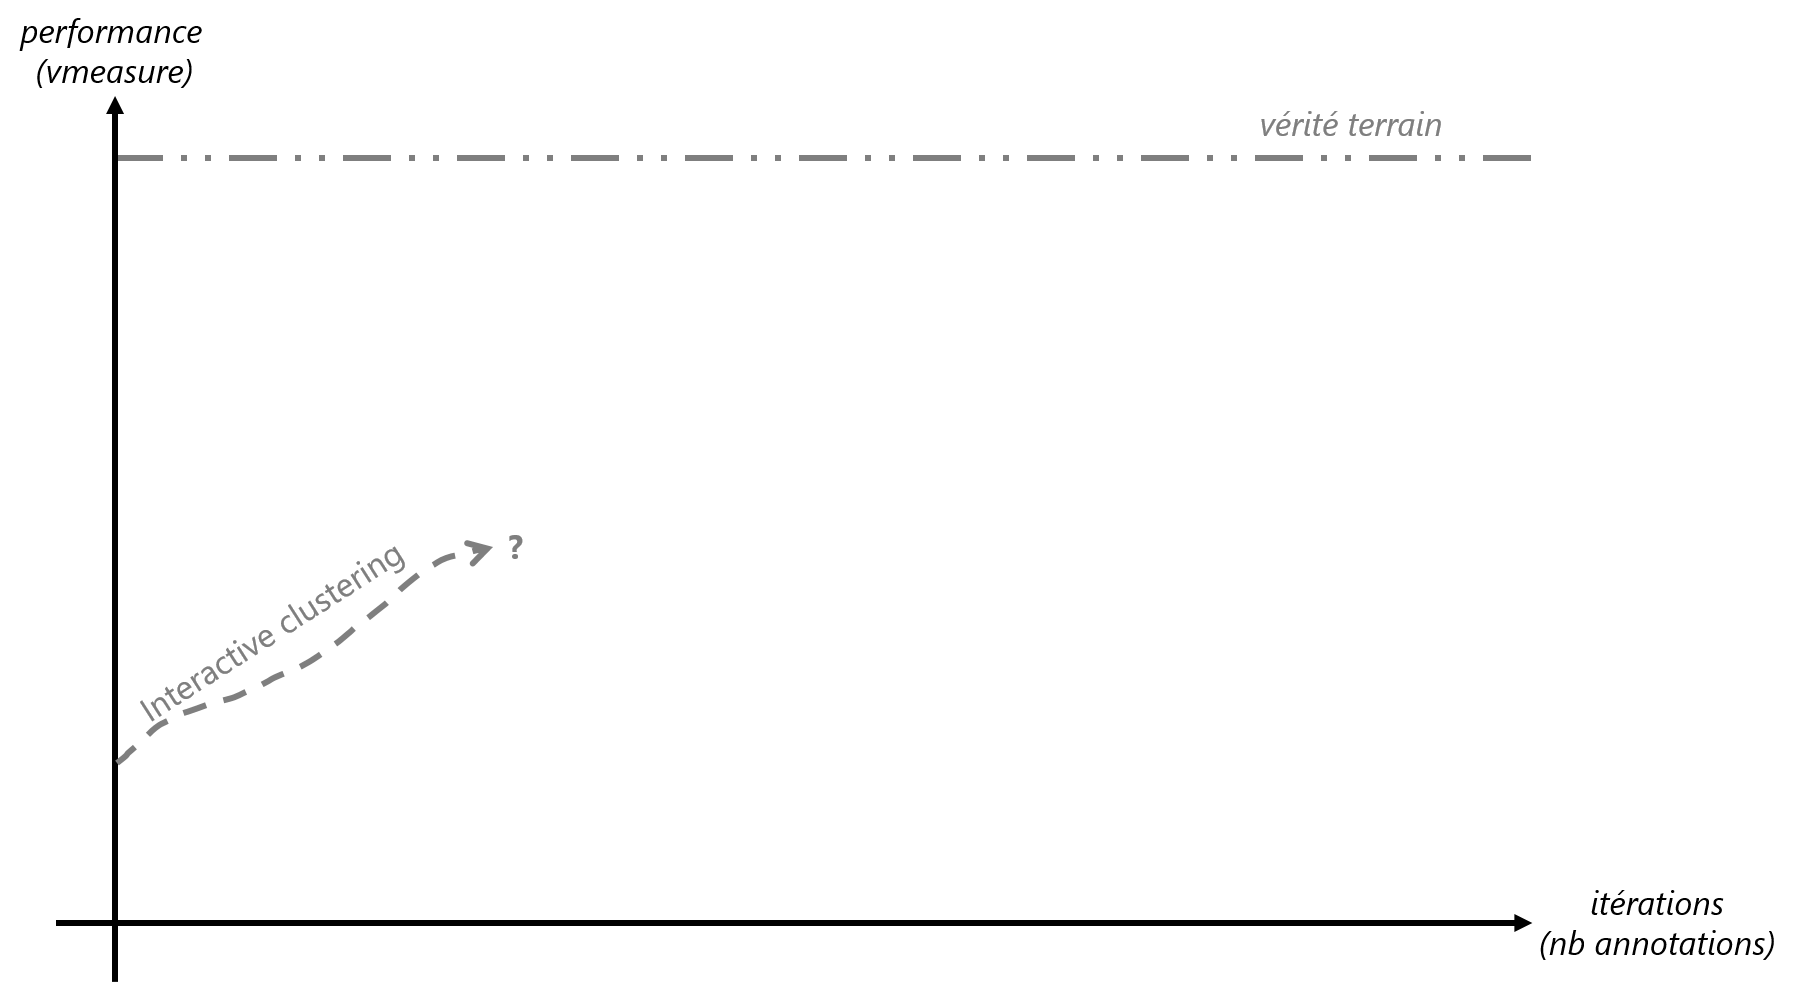
\includegraphics[width=0.95\textwidth]{figures/hypotheses-00-default}
		\caption{
			Illustration des études réalisées sur le \textit{clustering} interactif (\textit{étape 0/6}) en schématisant l'évolution de la performance (\textit{accord avec la vérité terrain calculé en v-measure}) d'une base d'apprentissage en cours de construction en fonction du nombre d'itérations de la méthode (\textit{nombre d'annotations par un expert métier}).
		}
		\label{figure:4.0-HYPOTHESE-00-DEFAULT}
	\end{figure}
	
	\todo[inline]{
		Pour ces études, nous allons (1) faire des analyses théoriques (2) des analyses empiriques (car dans la vrai vie on n'a pas de vérité terrain).
		Nous utilisons aussi la vmeasure.
	}
	\todo[inline]{
		Table des nomenclatures.
	}
	
	% PRÉAMBULE TECHNIQUE : CPU + scrips + datasets.
	\begin{leftBarInformation}
		Pour ces études, l'exécution des différentes expériences a été réalisée sur des CPU \texttt{Intel(R) Xeon(R) CPU E5-2660 v4 \@ 2.00GHz} et parallélisé avec la librairie Python \textit{multiprocessing} (un worker par CPU).
		Les scripts d'exécution et d'analyse de ces expériences, rédigés au sein de \textit{notebooks} Python (\cite{van-rossum-drake:2009:python-reference-manual}) ou de script R (\cite{r-core-team:2017:language-environment-statistical}), sont disponibles dans~\cite{schild:2021:cognitivefactory-interactiveclusteringcomparativestudy}.
		Enfin, les jeux de données utilisés pour ces études sont détaillés en Annexe~\ref{annex:C-ANNEXE-DATASET}.
	\end{leftBarInformation}
	
	
	% TABLE DES MATIÈRES DU CHAPITRE
	\minitoc
	
	%%%%%--------------------------------------------------------------------
	%%%%% Section 4.1: Hypothèse d'efficacité.
	%%%%%--------------------------------------------------------------------
	\newpage
	\section{Évaluation de l'hypothèse d'efficacité}
\label{section:4.1-HYPOTHESE-EFFICACITE}
%  : « \textit{est-ce que la méthode permet d'annoter un jeu de données ?} »
	
	%%% Formulation des hypothèses:
	Nous aimerions vérifier l'hypothèse suivante :

	\begin{tcolorbox}[
		title=\faVial~\textbf{Hypothèse d'efficacité}~\faVial,
		colback=colorTcolorboxHypothesis!15,
		colframe=colorTcolorboxHypothesis!75,
		width=\linewidth
	]
		% Hypothèse.
		« \textbf{
			Une méthodologie d'annotation basée sur le \textit{clustering} interactif permet d'obtenir une base d'apprentissage pour un assistant conversationnel qui respecte la vision donnée par l'expert métier au cours de l'annotation.
		} » \\
		
		% Résumé de l'étude.
		Afin de vérifier cette hypothèse, nous mettrons en place une expérience de ré-annotation d'une base d'apprentissage (qui servira ici de vérité terrain) à l'aide de notre méthode, en simulant l'annotation d'un expert, et nous critiquerons l'évolution de la nouvelle base d'apprentissage obtenue et sa similitude avec la base d'apprentissage initiale.
		
		% Figure.
		La figure~\ref{figure:4.1-HYPOTHESE-EFFICACITE} illustre cette hypothèse et l'espoir de convergence d'une base d'apprentissage en cours de construction vers sa vérité terrain.
		%
		\begin{figure}[H]  % keep [H] to be in the tcolorbox.
			\centering
			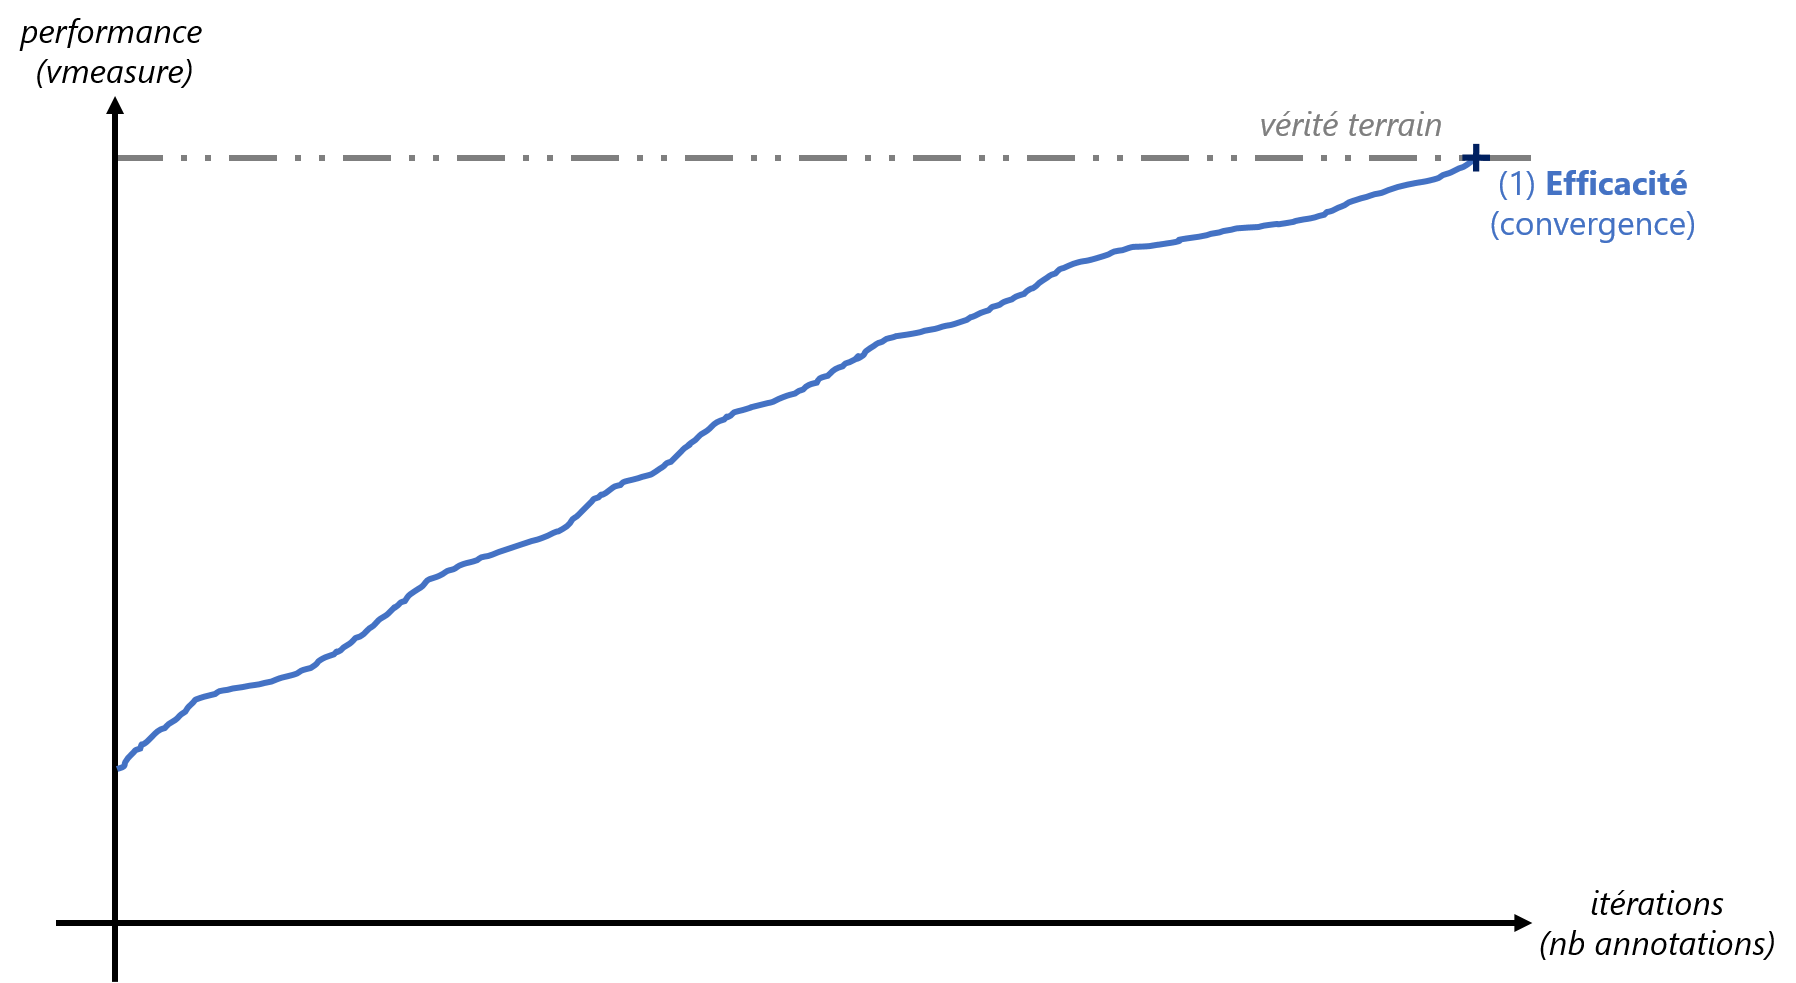
\includegraphics[width=0.8\textwidth]{figures/hypotheses-01-efficacite}
			\caption{Illustration des études réalisées sur le \textit{clustering} interactif (\textit{étape 1/6}) en schématisant l'évolution de la performance (\textit{accord avec la vérité terrain calculé en v-measure}) d'une base d'apprentissage en cours de construction en fonction du nombre d'itérations de la méthode (\textit{nombre d'annotations par un expert métier}).}
			\label{figure:4.1-HYPOTHESE-EFFICACITE}
		\end{figure}

	\end{tcolorbox}
	
	%%%
	%%% Subsection 4.1.1: Étude de convergence
	%%%
	\subsection{Étude de convergence vers une vérité terrain pré-établie}
	\label{subsection:4.1.1-ETUDE-CONVERGENCE}
			
		% Référence articles.
		\begin{leftBarInformation}
			Cette étude a été l'objet d'une présentation à la conférence \texttt{EGC (Extraction et Gestion des Connaissances)}~\citep{schild:conception-interactive-clustering:2021}, et d'une extension dans le journal \texttt{IJDWM (International Journal of Data Warehousing and Mining)}~\citep{schild:extension-interactive-clustering:2022}.
			\footnote{Les résultats et la discussion ont été mis à jour et réécrits pour mieux s'intégrer au discours ce manuscrit.}
		\end{leftBarInformation}

		%%% Protocole expérimental.
		\subsubsection{Protocole expérimental : simuler l'annotation d'une base d'apprentissage}
		
			% Objectif de l'expérience.
			Nous voulons vérifier qu'une méthodologie d'annotation basée sur notre implémentation du \textit{clustering} interactif permet de créer une base d'apprentissage pour un assistant conversationnel.
			Pour cela, nous prenons une base d'apprentissage employée pour entraîner un modèle de classification de textes\todo{référence, lien vers ANNEXE, + description conditions de création du JDD}, et nous utilisons ce jeu de données comme vérité terrain.
			L'objectif de cette expérience est de simuler la création de cette base d'apprentissage et de nous assurer que le résultat obtenu correspond à la vérité terrain.
			
			% Axiome.
			\begin{leftBarWarning}
				Dans le cadre de cette étude, nous supposons que l'expert métier connaît parfaitement le domaine traité dans ce jeu de données, et qu'il est capable de caractériser sans ambiguïté la similitude entre deux données issues de cet ensemble.
			\end{leftBarWarning}
			
			% Détails de l'expérience.
			Lors de cette expérience, chaque tentative de la méthode commencera sur la version non labellisée de la vérité terrain à disposition, sans aucune contrainte connue à l'avance.
			Au fur et à mesure des itérations de la méthode, nous simulerons l'annotation de l'expert métier en comparant les labels de la vérité terrain : ainsi, deux données ont une contrainte \texttt{MUST-LINK} si elles ont le même label, et une contrainte \texttt{CANNOT-LINK} sinon. Cela traduit le prérequis d'avoir un annotateur qui soit capable, dans son domaine d'expertise,  de différencier deux données selon leur ressemblance.
			Une tentative de l'application de notre méthode s'arrête lorsque toutes les contraintes possibles entre les données ont été annotés par l'expert.

			% Description implémentation de l'interactive clustering.
			Pour cette étude, nous essayons une tentative pour chaque combinaison de paramètre de notre implémentation du clustering interactif (cf. section~\ref{section:3.3-DESCRIPTION-IMPLEMENTATION}). Cela comprend les tâches et leurs paramètres respectifs suivants :
			%
			\begin{enumerate}
				\item le \textbf{prétraitement} des données, avec les niveaux suivants : \textbf{absent} (\texttt{prep.no}), \textbf{simple} (\texttt{prep.simple}), \textbf{avec lemmatisation} (\texttt{prep.lemma}) et \textbf{avec filtres} (\texttt{prep.filter}) ;
				\item la \textbf{vectorisation} des données, avec les niveaux suivants : \textbf{TF-IDF} (\texttt{vect.tfidf}) et \textbf{SpaCy} (\texttt{vect.frcorenewsmd}) ;
				\item le \textbf{clustering sous contraintes} des données, avec les niveaux suivants : \textbf{KMeans} (modèle \textit{COP} : \texttt{clust.kmeans.cop}), \textbf{Hiérarchique} (lien \textit{single}: \texttt{clust.hier.sing} ; lien \textit{complete} \texttt{clust.hier.comp} ; lien \textit{average} : \texttt{clust.hier.avg} ; lien \textit{ward} : \texttt{clust.hier.ward}) et \textbf{Spectral} (modèle \textit{SPEC} : \texttt{clust.spec}). Le choix du nombre de clusters n'est pas étudié ici, et ce nombre est fixé au nombre de classes présentes dans la vérité terrain ;
				\item l'\textbf{échantillonnage} des contraintes à annoter, avec les niveaux suivants : \textbf{purement aléatoire} (\texttt{samp.random.full}), \textbf{pseudo-aléatoire} (\texttt{samp.random.same}), \textbf{même cluster et étant les plus éloignées} (\texttt{samp.farhtest.same}) et \textbf{clusters différents et étant les plus proches} (\texttt{samp.closest.diff}). La choix de la taille d'échantillon n'est pas étudié ici, et cette taille est arbitrairement fixé à \texttt{50}.
			\end{enumerate}
			
			Il y a donc \texttt{192} combinaisons testées, et chaque tentative est répétée \texttt{5} fois pour contrer les aléas statistiques de certains algorithmes.
			Pour plus de détails sur ces algorithmes, référez-vous à la section~\ref{section:3.3-DESCRIPTION-IMPLEMENTATION} pour avoir accès à leur description, à leurs paramètres et aux choix d'implémentation.
			
			% Description de l'évaluation.
			Pour évaluer l'équivalence entre la vérité terrain et notre segmentation des données obtenue au cours de la méthode, nous nous intéresserons à l'évolution de la \texttt{v-measure} entre ces deux jeu de données.
			Si le score du calcul de la \texttt{v-measure} est de \texttt{100\%}, cela signifierait que le clustering final et la vérité terrain propose une segmentation identique des données, donc que la vérité terrain a pu être retrouvée, et donc qu'il est possible d'obtenir une base d'apprentissage pour un assistant conversationnel à l'aide d'une méthodologie d'annotation basée sur le \textit{clustering} interactif.
			
			% Pseudo-code.
			Pour résumer ce protocole expérimental, vous pouvez vous référez au pseudo-code décrit dans Alg.~\ref{algorithm:4.1.1-ETUDE-CONVERGENCE-PROTOCOLE}.
			%
			\begin{algorithm}[!htb]
				\begin{algorithmic}[1]
					\Require jeu de données annoté (vérité terrain)
					\ForAll{arrangement d'algorithmes et de paramètres à tester}
						\State \textbf{initialisation}: récupérer les données de la vérité terrain sans leur label, créer une liste vide de contraintes
						\State \textbf{prétraitement}: supprimer le bruit dans les données
						\State \textbf{vectorisation}: transformer les données en vecteurs
						\State \textbf{clustering initial}: regrouper les données par similarité
						\State \textbf{évaluation}: estimer l'équivalence entre le clustering obtenu et la vérité terrain
						\Repeat
							\State \textbf{échantillonnage}: sélectionner de nouvelles contraintes à annoter
							\State \textbf{simulation d'annotation}: ajouter des contraintes grâce à la comparaison des labels de la vérité terrain
							\State \textbf{clustering}: regrouper les données par similarité avec les contraintes
							\State \textbf{évaluation}: estimer l'équivalence entre le clustering obtenu et la vérité terrain
						\Until{annotation de toutes les contraintes possibles}
						\State \textbf{évaluation finale}: espérer avoir un score d'équivalence de 100\% entre le clustering obtenu et la vérité terrain
					\EndFor
					\Ensure arrangements d'algorithmes et de paramètres ayant un score d'équivalence de 100\%
				\end{algorithmic}
				\caption{Description en pseudo-code du protocole expérimental de l'étude de convergence du \textit{clustering} interactif vers une vérité terrain pré-établie.}
				\label{algorithm:4.1.1-ETUDE-CONVERGENCE-PROTOCOLE}
			\end{algorithm}
			
			% Référence scripts.
			\begin{leftBarInformation}
				Les scripts de l'expérience (\textit{notebooks} Python) sont disponibles dans un dossier dédié de~\cite{schild:cognitivefactory-interactive-clustering-comparative-study:2021}.
			\end{leftBarInformation}

		%%% Résultats.
		\subsubsection{Résultats obtenus}
			
			% Graphe d'évolution de la v-measure moyenne, min et max.
			La figure~\ref{figure:4.1.1-ETUDE-CONVERGENCE-EVOLUTION} et le tableau~\ref{table:4.1.1-ETUDE-CONVERGENCE-EVOLUTION} représentent l'évolution moyenne de la \texttt{v-measure} du clustering en fonction du nombre d'itération de la méthode. Les tentatives les plus rapides et les plus lentes sont représentées sur la figure.
							
			% Tendance: Forte dispersion, Croissance générale.
			Malgré une forte dispersion des résultats (écart-type de \texttt{v-measure} pouvant être supérieur à 20\%, forte différence entre les tentatives la plus rapide et la plus lente) et quelques sauts de performances (cf. à-coups de la tentative la plus lente sur la figure), une convergence générale vers la vérité terrain peut être constatée.
			
			% Tendance à courts termes: Croissance linéaire
			A l'itération \texttt{0}, une tentative commence avec une moyenne de \texttt{19.05}\% de \texttt{v-measure}  entre son \textit{clustering} initial (sans contraintes) et la vérité terrain.
			Cette \texttt{v-measure} moyenne croît presque linéairement (pente de \texttt{0.97}) jusqu'à l'itération 75 où elle atteint la performance de \texttt{92.08}\% (cf. tableau~\ref{table:4.1.1-ETUDE-CONVERGENCE-EVOLUTION}).

			% Tendance à longs termes: Asymptote.
			Au delà de l'itération 75, la courbe de la \texttt{v-measure} moyenne tend vers une asymptote de {100}\% (cf. figure~\ref{figure:4.1.1-ETUDE-CONVERGENCE-EVOLUTION}).
			Cette asymptote est atteinte par toute les \texttt{960} tentatives (\texttt{192} combinaisons de paramètres, \texttt{5} tentatives pour chaque combinaison), la tentative l'ayant atteinte le plus tôt à l'itération 19 et celle le plus tard à l'itération 326.
			La courbe se prolonge jusqu'à l'itération \texttt{394} pour que toutes les tentatives puisse annoter toutes les contraintes possibles sur le jeu de données.
			
			%
			\begin{figure}[!htb]
				\centering
				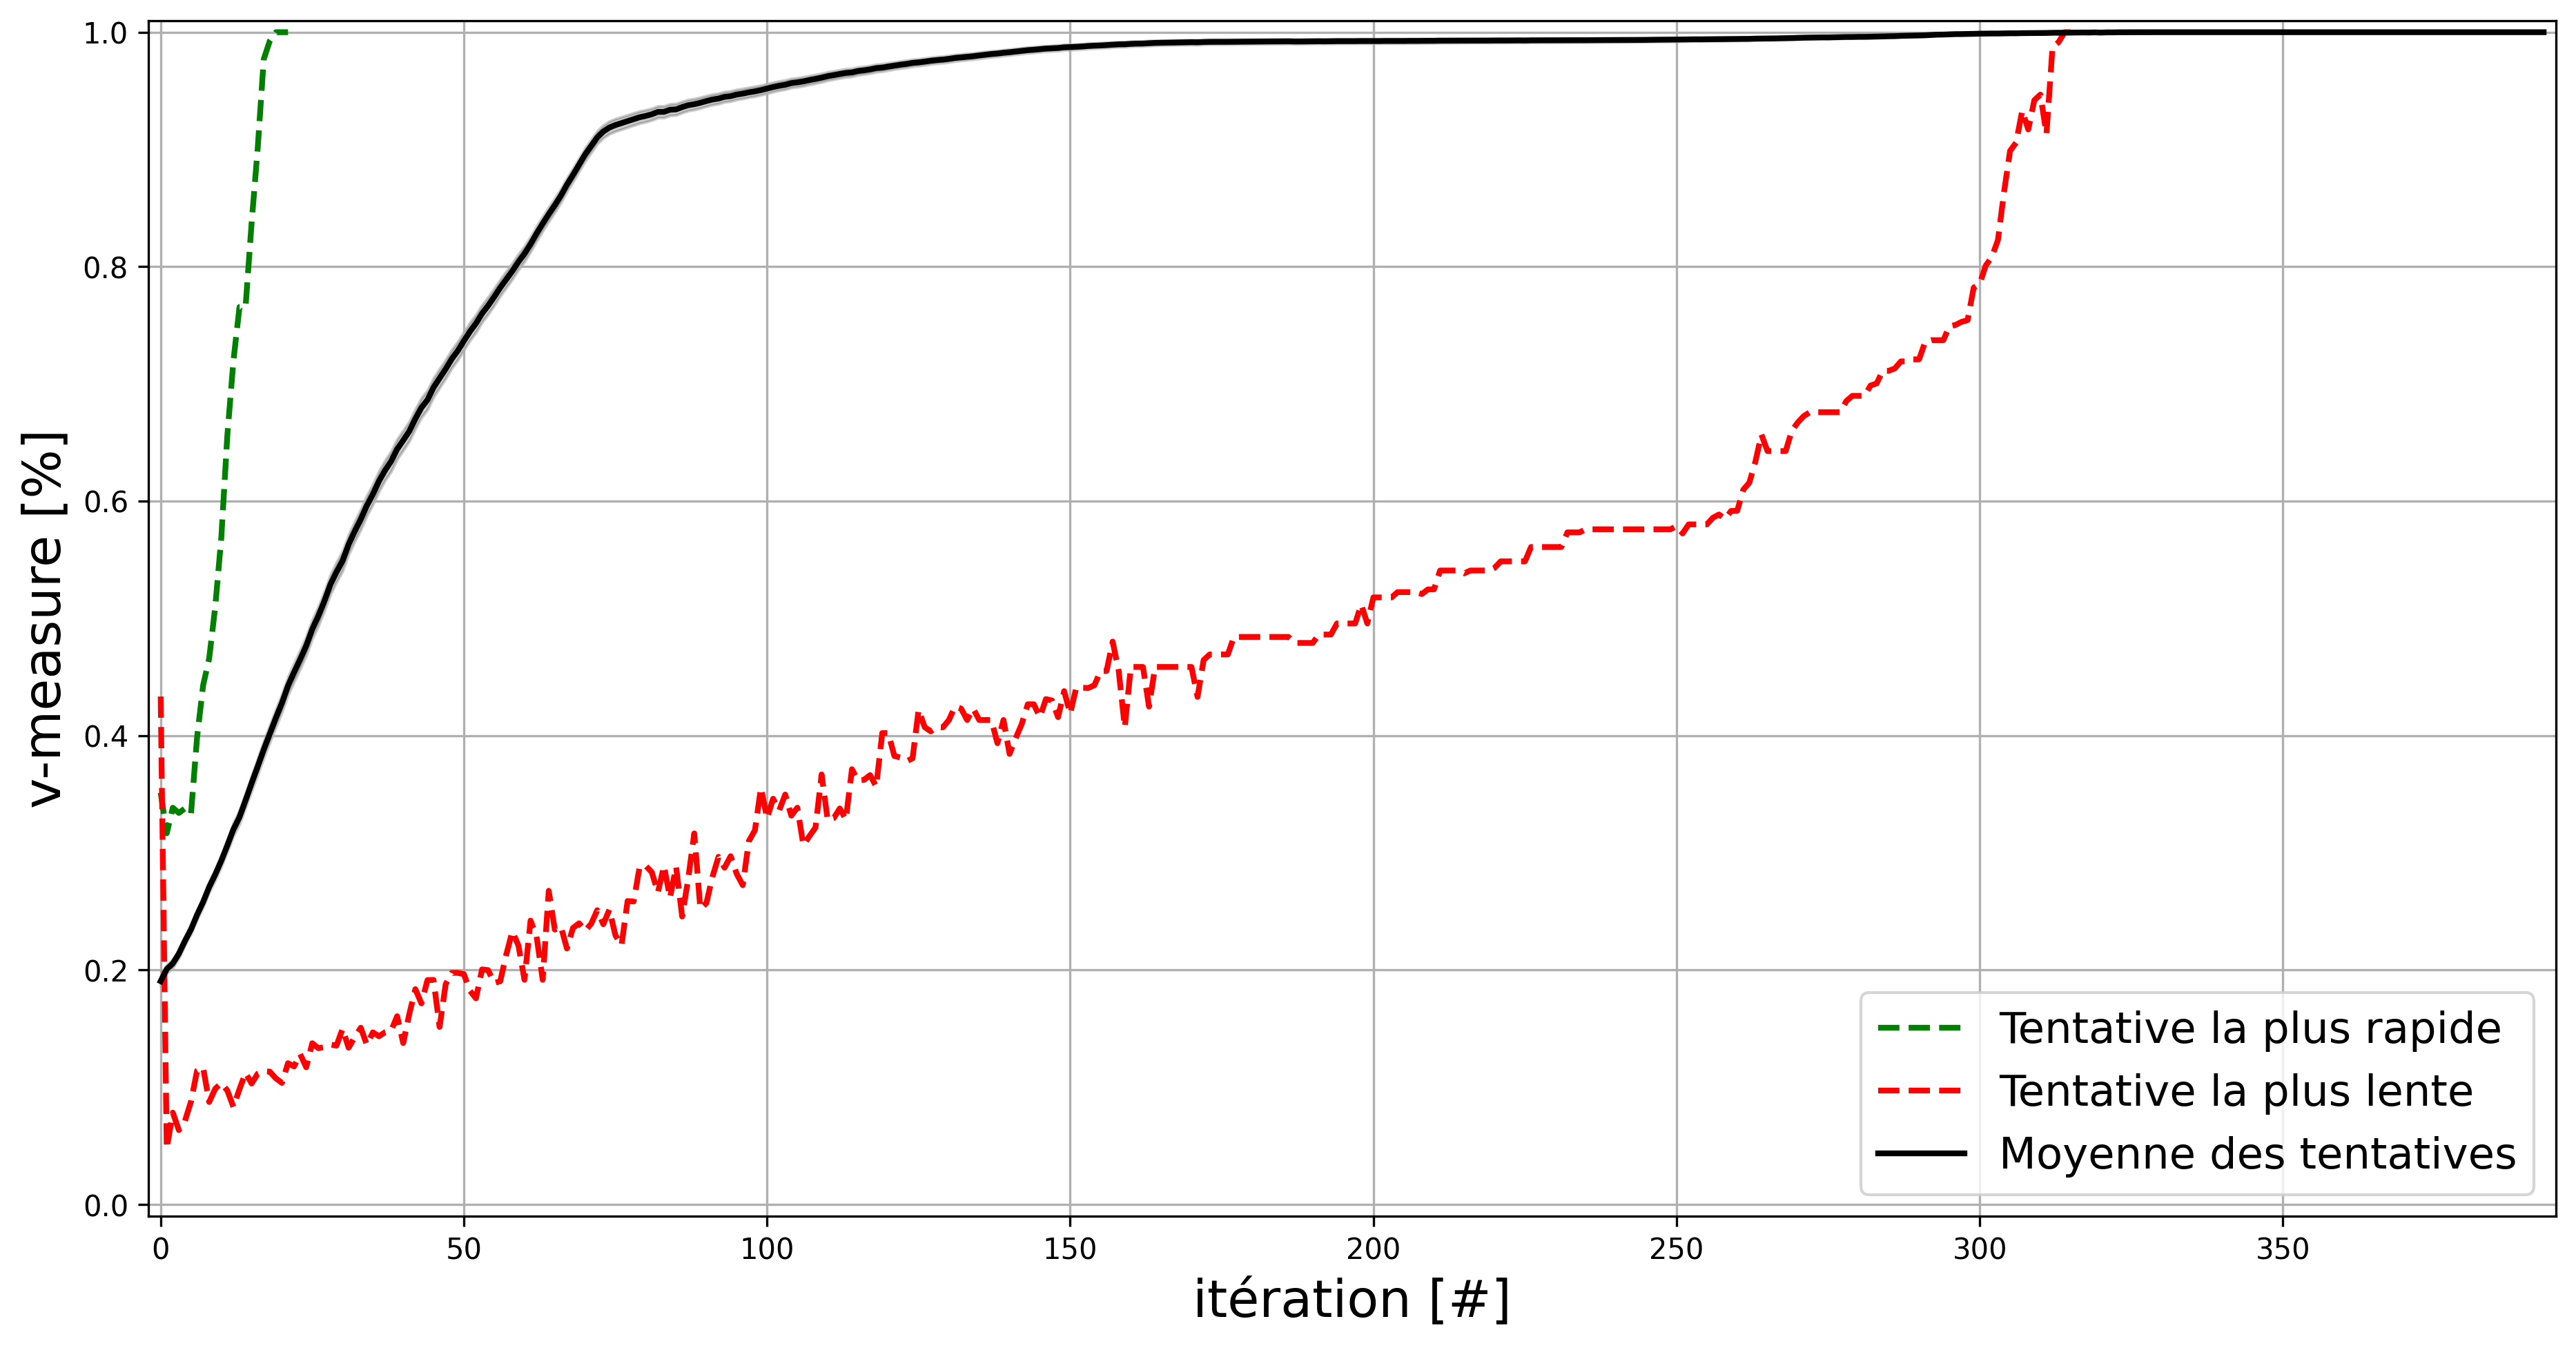
\includegraphics[width=0.8\textwidth]{figures/etude-efficacite-evolution-moyenne-0par-iteration}
				\caption{Évolution de la moyenne de la \texttt{v-measure} entre un résultat obtenu et la vérité terrain en fonction du nombre d'itération de la méthode de \textit{clustering} interactif, moyenne réalisée itération par itération sur l'ensemble des tentatives.
				Représentation des tentatives ayant été les plus rapides (\textit{un prétraitement \texttt{prep.simple}, une vectorisation \texttt{vect.tfidf}, un clustering \texttt{clust.hier.comp} ou \texttt{clust.hier.ward}, et un échantillonnage \texttt{samp.closest.diff}}) et les plus lentes (\textit{un prétraitement \texttt{prep.no}, une vectorisation \texttt{vect.tfidf}, un clustering \texttt{clust.spec}, et un échantillonnage de contraintes \texttt{samp.farthest.same}}) pour atteindre 100\% de \texttt{v-measure}.}
				\label{figure:4.1.1-ETUDE-CONVERGENCE-EVOLUTION}
			\end{figure}
			%
			\begin{table}[!htb]
				\begin{center}
				\begin{tabular}{|c|r|r|r|r|r|}
					\hline
					% ENTETE DU TABLEAU
					\multicolumn{2}{|c|}{ \shortstack{ Annotations } }
						& \multicolumn{4}{c|}{ \shortstack{ Performances (\texttt{v-measure}) } }
						\tabularnewline
						\hline
					\multicolumn{1}{|c|}{ \shortstack{ Itérations } }
						& \multicolumn{1}{c|}{ \shortstack{ Contraintes } }
						& \multicolumn{1}{c|}{ \shortstack{ Moyenne } }
						& \multicolumn{1}{c|}{ \shortstack{ Écart-type } }
						& \multicolumn{1}{c|}{ \shortstack{ Minimum } }
						& \multicolumn{1}{c|}{ \shortstack{ Maximum } }
						\tabularnewline
						\hline
					%
					0	& 0		& \( 19.05\% \) \footnotesize \( (\pm0.43) \) \par	& \( 13.38\% \) & \( 03.42\% \) & \( 47.75\% \)
					\tabularnewline
					\hline
					%
					25	& 1 250	& \( 49.09\% \) \footnotesize \( (\pm0.82) \) \par	& \( 25.43\% \) & \( 09.09\% \) & \( 100.00\% \)
					\tabularnewline
					\hline
					%
					50	& 2 500	& \( 73.66\% \) \footnotesize \( (\pm0.77) \)	 \par& \( 23.98\% \) & \( 16.78\% \) & \( 100.00\% \)
					\tabularnewline
					\hline
					%
					75	& 3 750	& \( 92.08\% \) \footnotesize \( (\pm0.54) \) \par	& \( 16.70\% \) & \( 21.74\% \) & \( 100.00\% \)
					\tabularnewline
					\hline
					%
					100	& 5 000	& \( 95.19\% \) \footnotesize \( (\pm0.41) \) \par	& \( 12.67\% \) & \( 26.93\% \) & \( 100.00\% \)
					\tabularnewline
					\hline
					%
					125	& 6 250	& \( 97.43\% \) \footnotesize \( (\pm0.29) \) \par	& \( 09.09\% \) & \( 34.99\% \) & \( 100.00\% \)
					\tabularnewline
					\hline
					%
					150	& 7 500	& \( 98.73\% \) \footnotesize \( (\pm0.23) \) \par	& \( 07.22\% \) & \( 38.14\% \) & \( 100.00\% \)
					\tabularnewline
					\hline
					
				\end{tabular}
				\end{center}
				\caption{Détails de l'évolution de la moyenne de la \texttt{v-measure} entre un résultat obtenu et la vérité terrain en fonction du nombre d'itération de la méthode de \textit{clustering} interactif, moyenne réalisée itération par itération sur l'ensemble des tentatives.}
				\label{table:4.1.1-ETUDE-CONVERGENCE-EVOLUTION}
			\end{table}

		%%% Discussion
		\subsubsection{Discussion}
			
			%%% Principale conclusion : il y a convergence !
			La première et principale conclusion de cette étude concerne la preuve que la méthode est efficace.
			En effet, les différentes simulations ont bien convergé vers la vérité terrain (atteinte de l'asymptote à \texttt{100}\% de \texttt{v-measure}), montrant qu'il est possible pour un expert métier de créer une base d'apprentissage à l'aide d'une méthodologie d'annotation basée sur le \textit{clustering} interactif. \\
			
			
			%%% Avantages.
			Cette découverte permet de confirmer plusieurs espoirs portés sur la méthode. 
			
			% Avantage 1 : Émergence d'une modélisation sur la base des contraintes
			Tout d'abord, la vérité terrain a été retrouvée sans formaliser concrètement la structure de données.
			Là où une annotation par label aurait requis au préalable une définition des catégories possibles pour les données à étiqueter, la méthodologie employant le \textit{clustering} interactif a permis de faire émerger naturellement cette structure de données.
			Cette émergence provient directement des contraintes annotées par l'expert métier, traduisant ainsi ses connaissances à l'aide d'instructions simples : \textit{les données sont-elles ou non similaires ?}
			
			% Avantage 2 : annotations plus simples et plus concrètes
			De plus, ces contraintes ont été l'objet d'une annotation guidée par les besoins de la machine afin de s'améliorer d'itération en itération (voir la croissance globale de la \texttt{v-measure} sur la figure~\ref{figure:4.1.1-ETUDE-CONVERGENCE-EVOLUTION}).
			Ainsi, l'expert métier corrige la base d'apprentissage à chaque itération : soit en affinant les clusters en cours de construction, améliorant ainsi la cohérence des clusters (cf. pentes croissantes) ; soit en remaniant les clusters mal formés pour repartir sur de bonnes bases, détériorant la cohérence des clusters le temps de la réorganisation (cf. oscillations ou pentes décroissantes). \\

			
			%%% Limites.
			Néanmoins, différentes pistes sont encore à explorer pour rendre le \textit{clustering} interactif utilisable en situation réelle.
			
			% Limite 1 : Nombre d'annotations ==> besoin d'optimisation.
			D'une part, nous échangeons le besoin de définir une structure de données contre la nécessité d'annoter un grand nombre de contraintes : pour \texttt{500} points de données, et en considérant que l'asymptote à \texttt{100}\% est atteinte en moyenne autour de l'itération \texttt{200}, il faudrait \texttt{10 000} annotations de contraintes pour être exhaustif, ce qui correspond à près de \texttt{20} fois plus de contraintes que de données.
			Bien que l'annotation binaire demande a priori une charge mentale plus faible à un annotateur, un tel volume représente tout de même une grande quantité de travail.
			\todo{
				Commentaire Gautier 22/05/2023 :
				(A DÉTAILLER AILLEURS ?)
				Oui, complètement d'accord ici, mais en fait ça va plus loin que ça non ?
				Déjà, on a une quantité de ressources allouées à la tâche en effet plus fabile (car choisir entre "similaire" et "non similaire" est clairement plus simple que d'assigner un label parmi N).
				Mais on a aussi une diminution des ressources allouées au maintien d'une stratégie d'annotation : en effet, pas besoin de définir à l'avance de type system ou autre, tout est construit à la volée. Ce deuxième point est particulierement intéressant à discuter je pense, car on sait normalement que le maintien d'objectifs en mémoire de travail peut aider à maintenir un niveau d'engagement sur une tâche cognitive. Du coup, ça pose d'autant plus la question de l'expérience utilisateur : annoter avec un CI sera-t-il moins engageant qu'annoter avec une méthode classique ?
			}
			Cela peut décourager les experts métiers en début de projet, surtout pour des projets ayant des jeux de données de plus grandes tailles.
			Toutefois, les résultats obtenus montrent une forte dispersion du nombre d'itérations nécessaire, et certaines tentatives ont été bien plus efficientes dans l'utilisation de leurs contraintes. La tentative la plus rapide a convergé à l'itération \texttt{19}, soit \texttt{950} contraintes, ce qui est un volume d'annotation bien plus abordable !
			On peut donc espérer trouver un paramétrage optimal de la méthode permettant de diminuer significativement le nombre moyen de contraintes nécessaires afin d'obtenir une base d'apprentissage exploitable avec un volume d'annotations acceptable.
			Cet aspect fait l'objet de l'étude décrite dans la section~\ref{section:4.2-HYPOTHESE-EFFICIENCE} (hypothèse d'efficience).
			
			% Limite 2 : Exhaustivité des annotations ==> evaluation de la rentabilité.
			D'autre part, le choix d'annoter toutes les contraintes possibles sur les données (\textbf{annotation exhaustive}) n'est pas forcément judicieux.
			En effet, si nous nous référons à la figure~\ref{figure:4.1.1-ETUDE-CONVERGENCE-EVOLUTION}), une moyenne de \texttt{90}\% de \texttt{v-measure} est déjà atteinte autour de l'itération \texttt{75}, alors que l'asymptote à \texttt{100}\% n'est atteinte qu'au delà de l'itération \texttt{200}. Afin d'être plus efficient, il faudrait envisager une \textbf{annotation partielle} permettant d'obtenir rapidement \texttt{90}\% de \texttt{v-measure} (quitte à affiner le résultat manuellement pour combler la "perte" moyenne de \texttt{10}\% de \texttt{v-measure}).
			Cet aspect sera ajouté à l'objectif de l'étude décrite dans la section~\ref{section:4.2-HYPOTHESE-EFFICIENCE} (hypothèse d'efficience).
			
			% Limite 3 : Expert métier parfait ==> simuler les erreurs.
			Pour finir, nous avons supposé dans cette étude que l'annotateur est un expert métier connaissant parfaitement le domaine traité.
			Cette hypothèse forte n'est a priori pas valable en situation réelle : En effet, des erreurs d'annotations peuvent intervenir (ambiguïtés sur les données, méconnaissance du domaine, erreurs d'inattention, différence d'opinions entre annotateurs, ...), ce qui peut entraîner des divergences ou des incohérences dans la construction de la base d'apprentissage.
			Il semble donc nécessaire d'étudier les impacts de ces incohérences, ainsi que de proposer une méthode pour les prévenir ou les corriger.
			Cet aspect sera traité à la fin de ce chapitre dans la section~\ref{section:4.6-HYPOTHESE-ROBUSTESSE} (hypothèse de robustesse).
	
	
	%%%%%--------------------------------------------------------------------
	%%%%% Section 4.2: Hypothèse d'efficience.
	%%%%%--------------------------------------------------------------------
	\newpage
	\section{Évaluation de l'hypothèse d'efficience}
\label{section:4.2-HYPOTHESE-EFFICIENCE}

	%%% Introduction / Transition.
	Suite à la validation de l'hypothèse d'efficacité (convergence de la méthode, cf. section~\ref{section:4.1-HYPOTHESE-EFFICACITE}), nous déterminer les paramètres optimaux de la méthodes afin de converger le plus rapidement vers la vérité terrain.
	Nous aimerions donc vérifier l'hypothèse suivante :

	%%% Formulation des hypothèses:
	\begin{tcolorbox}[
		title=\faVial~\textbf{Hypothèse d'efficience}~\faVial,
		colback=colorTcolorboxHypothesis!15,
		colframe=colorTcolorboxHypothesis!75,
		width=\linewidth
	]

		% Hypothèse.
		« \textbf{
			La vitesse de convergence du \textit{clustering} interactif peut être optimisée en ajustant différents paramètres afin de minimiser la charge de travail de l'opérateur.
			Nous étudierons en particulier l'influence sur le nombre de contraintes requis du prétraitement des données, de la vectorisation des données, de l'échantillonnage des contraintes à annoter et du \textit{clustering} sous contraintes.
		} » \\
		
		% Résumé de l'étude.
		Afin de vérifier cette hypothèse, nous mettrons en place une expérience de ré-annotation d'une base d'apprentissage (qui servira ici de vérité terrain) à l'aide de notre méthode, en simulant l'annotation d'un expert, et nous réaliserons l'analyse statistique de la taille d'effet de différents paramètres sur la vitesse de convergence du \textit{clustering} itératif.
		
		% Figure.
		La figure~\ref{figure:4.2-HYPOTHESE-EFFICIENCE} illustre cette hypothèse et l'espoir d'une convergence "optimale" d'une base d'apprentissage en cours de construction vers sa vérité terrain.
		%
		\begin{figure}[H]  % keep [H] to be in the tcolorbox.
			\centering
			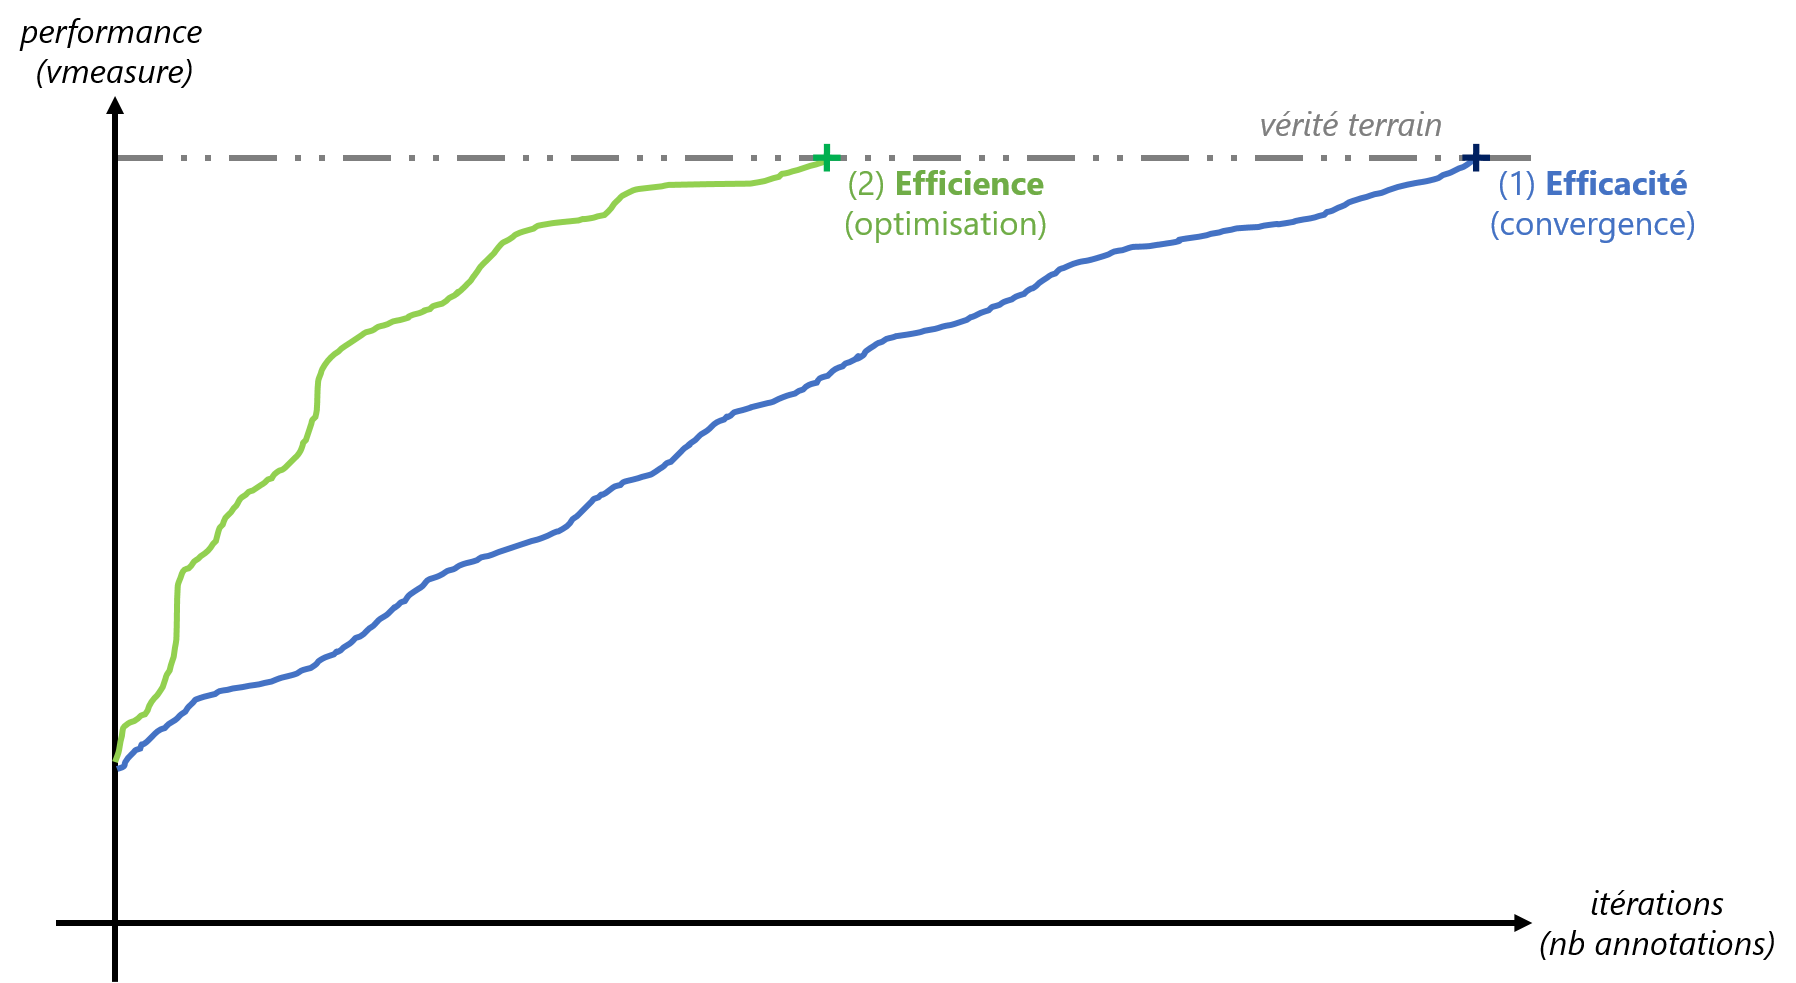
\includegraphics[width=0.95\textwidth]{figures/hypotheses-02-efficience}
			\caption{Illustration des études réalisées sur le \textit{clustering} interactif (\textit{étape 2/6}) en schématisant l'évolution de la performance (\textit{accord avec la vérité terrain calculé en v-measure}) d'une base d'apprentissage en cours de construction en fonction du nombre d'itérations de la méthode (\textit{nombre d'annotations par un expert métier}).}
			\label{figure:4.2-HYPOTHESE-EFFICIENCE}
		\end{figure}

	\end{tcolorbox}
	
	%%%
	%%% Subsection 4.2.1: Étude d'optimisation des paramètres d’implémentation en analysant leurs tailles d'effets sur la vitesse de création d'une base d'apprentissage.
	%%%
	\subsection{Étude d'optimisation des paramètres d’implémentation en analysant leurs tailles d'effets sur la vitesse de création d'une base d'apprentissage}
	\label{section:4.2.1-ETUDE-OPTIMISATION}
			
		% Référence articles.
		\begin{leftBarInformation}
			Cette étude a été l'objet d'une présentation à la conférence \texttt{EGC (Extraction et Gestion des Connaissances)}~\citep{schild:conception-interactive-clustering:2021}, et d'une extension dans le journal \texttt{IJDWM (International Journal of Data Warehousing and Mining)}~\citep{schild:extension-interactive-clustering:2022}.
			\footnote{Les résultats et la discussion de ces articles ont été mis à jour et réécrits pour mieux s'intégrer au discours ce manuscrit.}
		\end{leftBarInformation}

		%%% Protocole expérimental.
		\subsubsection{Protocole expérimental}

			% Objectif de l'expérience.
			Nous voulons étudier l'influence des paramètres de notre implémentation du \textit{clustering} interactif sur la vitesse de création d'une base d'apprentissage pour un assistant conversationnel.
			Nous allons donc compléter le protocole expérimental de l'étude de convergence en section~\ref{section:4.1.1-ETUDE-CONVERGENCE} visant à simuler la création d'une base d'apprentissage.
			
			% Axiome.
			\begin{leftBarWarning}
				Comme dans l'étude précédente, nous supposons que l'expert métier connaît parfaitement le domaine traité dans ce jeu de données, et qu'il est capable de caractériser sans ambiguïté la similitude entre deux données issues de cet ensemble.
				Cependant, cette hypothèse forte n'est pas toujours vérifiée en pratique, surtout lorsque l'on manipule des données non structurées.
				L'impact de ce point sur les résultats obtenus sera discuté en fin en fin de partie, et nous nous y intéresserons plus en détails dans la section~\ref{section:4.6-HYPOTHESE-ROBUSTESSE} (hypothèse de robustesse).
			\end{leftBarWarning}
			
			% Pseudo-code.
			Pour résumer le protocole expérimental adapté, vous pouvez vous référer au pseudo-code décrit dans Alg.~\ref{algorithm:4.2.1-ETUDE-OPTIMISATION-PROTOCOLE}.
			%
			\begin{algorithm}[!htb]
				\begin{algorithmic}[1]
					\Require jeu de données annoté (vérité terrain)
					\ForAll{arrangement d'algorithmes et de paramètres à tester}
						\State \textbf{initialisation (données)}: récupérer les données et la vérité terrain
						\State \textbf{initialisation (contraintes)}: créer une liste vide de contraintes
						\State \textbf{prétraitement}: supprimer le bruit dans les données
						\State \textbf{vectorisation}: transformer les données en vecteurs
						\State \textbf{clustering initial}: regrouper les données par similarité
						\State \textbf{évaluation}: estimer l'équivalence entre le \textit{clustering} obtenu et la vérité terrain
						\Repeat
							\State \textbf{échantillonnage}: sélectionner de nouvelles contraintes à annoter
							\State \textbf{simulation d'annotation}: ajouter des contraintes en utilisant la vérité terrain
							\State \textbf{clustering}: regrouper les données par similarité avec les contraintes
							\State \textbf{évaluation}: estimer l'équivalence entre le \textit{clustering} obtenu et la vérité terrain
						\Until{annotation de toutes les contraintes possibles}
					\EndFor
					\State \textbf{analyse}: déterminer les tailles d'effets des algorithmes et paramètres
					\Ensure meilleurs arrangements d'algorithmes et de paramètres
				\end{algorithmic}
				\caption{Description en pseudo-code du protocole expérimental de l'étude d'optimisation de la convergence du \textit{clustering} interactif vers une vérité terrain pré-établie.}
				\label{algorithm:4.2.1-ETUDE-OPTIMISATION-PROTOCOLE}
			\end{algorithm}
			
			% Détails de l'expérience.
			En s'appuyant sur les résultats précédemment obtenus,
			nous allons analyser l'influence des différentes tâches employées (\textbf{prétraitement}, \textbf{vectorisation}, \textbf{clustering sous contraintes}, \textbf{échantillonnage}) et de leurs paramètres sur la vitesse de convergence vers la vérité terrain.
			% Description implémentation de l'interactive clustering.
			Nous utilisons à nouveau le jeu de données \texttt{Bank Cards (v1.0.0)} (cf. annexe~\ref{annex:C.1-DATASET-BANK-CARDS}) comme vérité terrain, sur lequel nous testons $192$ combinaisons de paramétrage, et chaque tentative est répétée $5$ fois pour contrer les aléas statistiques de certains algorithmes.
			Pour plus de détails sur ces algorithmes, référez-vous à la section~\ref{section:3.3-DESCRIPTION-IMPLEMENTATION}.
			
			% Description de l'évaluation et Seuils d'évaluation.
			Comme lors de l'étude sur la convergence de la méthode, nous nous intéressons à l'évolution de la \texttt{v-measure} entre la vérité terrain et notre segmentation des données obtenue, et nous affinons notre évaluation en portant attention aux trois seuils d'annotations suivants :
			\begin{enumerate}
				\item le cas d'une \textbf{annotation partielle}, correspondant au nombre d'itérations nécessaires à la méthode pour avoir $90$\% de \texttt{v-measure}, c'est-à-dire un état de semi-parcours vers une convergence totale\footnote{Le seuil de $90$\% a été choisi au cours de l'étude de convergence (cf. hypothèse d'efficacité, section~\ref{section:4.1-HYPOTHESE-EFFICACITE}, coude de la figure~\ref{figure:4.1.1-ETUDE-CONVERGENCE-EVOLUTION}).} ;
				\item le cas d'une \textbf{annotation suffisante}, correspondant au nombre d'itérations nécessaires à la méthode pour avoir $100$\% de \texttt{v-measure}, c'est-à-dire avoir suffisamment de contraintes annotées par l'expert métier pour retrouver la vérité terrain ;
				\item le cas d'une \textbf{annotation exhaustive}, correspondant au nombre d'itérations nécessaires à la méthode pour parcourir toutes les contraintes possibles sur les données, et ainsi retranscrire exhaustivement la vision de l'expert métier\footnote{Une annotation est a priori inutilisable en pratique (demande trop de contraintes, cf. hypothèse d'efficacité, section~\ref{section:4.1-HYPOTHESE-EFFICACITE}), nous l'étudions toutefois pour avoir un point de comparaison.}.
			\end{enumerate}
			
			% Description de l'analyse ANOVA.
			Enfin, nous utilisons une \texttt{ANOVA} à mesures répétées afin de déterminer l’effet des paramètres de notre implémentation sur le nombre d’annotations requis pour converger vers la vérité terrain.
			
			% Référence scripts.
			\begin{leftBarInformation}
				Ces analyses sont réalisées à l'aide du logiciel R, et le test de \texttt{Tukey (HSD)} est utilisé pour les comparaisons post-hoc.
				Les scripts de l'expérience (\textit{notebooks} Python) sont disponibles dans un dossier dédié de~\cite{schild:cognitivefactory-interactive-clustering-comparative-study:2021}.
			\end{leftBarInformation}
			\todo{citation}

		%%% Résultats.
		\subsubsection{Résultats obtenus}
		
			%%% Analyse d'une annotation partielle.
			Pour obtenir une \textbf{annotation partielle} (\textit{atteindre une \texttt{v-measure} de $90$\%}), la moyenne des itérations est de $59.04$ (min: $11$, max: $315$, écart-type: $42.14$), soit une moyenne de $2~951.81$ annotations (min: $550$, max: $15~750$, écart-type: $2~106.72$).
			La figure~\ref{figure:4.2.1-ETUDE-OPTIMISATION-HISTOGRAMME-ANNOTATION-PARTIELLE} représente la répartition de ces itérations au cours des différentes tentatives.
			On peut noter les deux cas intéressants suivants :
			%
			\begin{itemize}
				\item[$\bullet$] Les tentatives les plus rapides furent celles avec un prétraitement des données \texttt{prep.no} ou \texttt{prep.simple} ou \texttt{prep.lemma}, une vectorisation des données \texttt{vect.tfidf}, un \textit{clustering} sous contraintes \texttt{clust.hier.sing}, et un échantillonnage de contraintes \texttt{samp.closest.diff}. Ces tentatives ont requis $11$ itérations, soit $550$ annotations, dont $299$ (respectivement $304$ et $281$) contraintes \texttt{MUST-LINK}.
				\item[$\bullet$] Les tentatives les plus lentes furent celles avec un prétraitement des données \texttt{prep.no}, une vectorisation des données \texttt{vect.tfidf}, un \textit{clustering} sous contraintes \texttt{clust.spec}, et un échantillonnage de contraintes \texttt{samp.farthest.same}. Ces tentatives ont requis $315$ itérations, soit $15~750$ annotations, dont $1~032$ contraintes \texttt{MUST-LINK}.
			\end{itemize}
			%
			\begin{figure}[!htb]
				\centering
				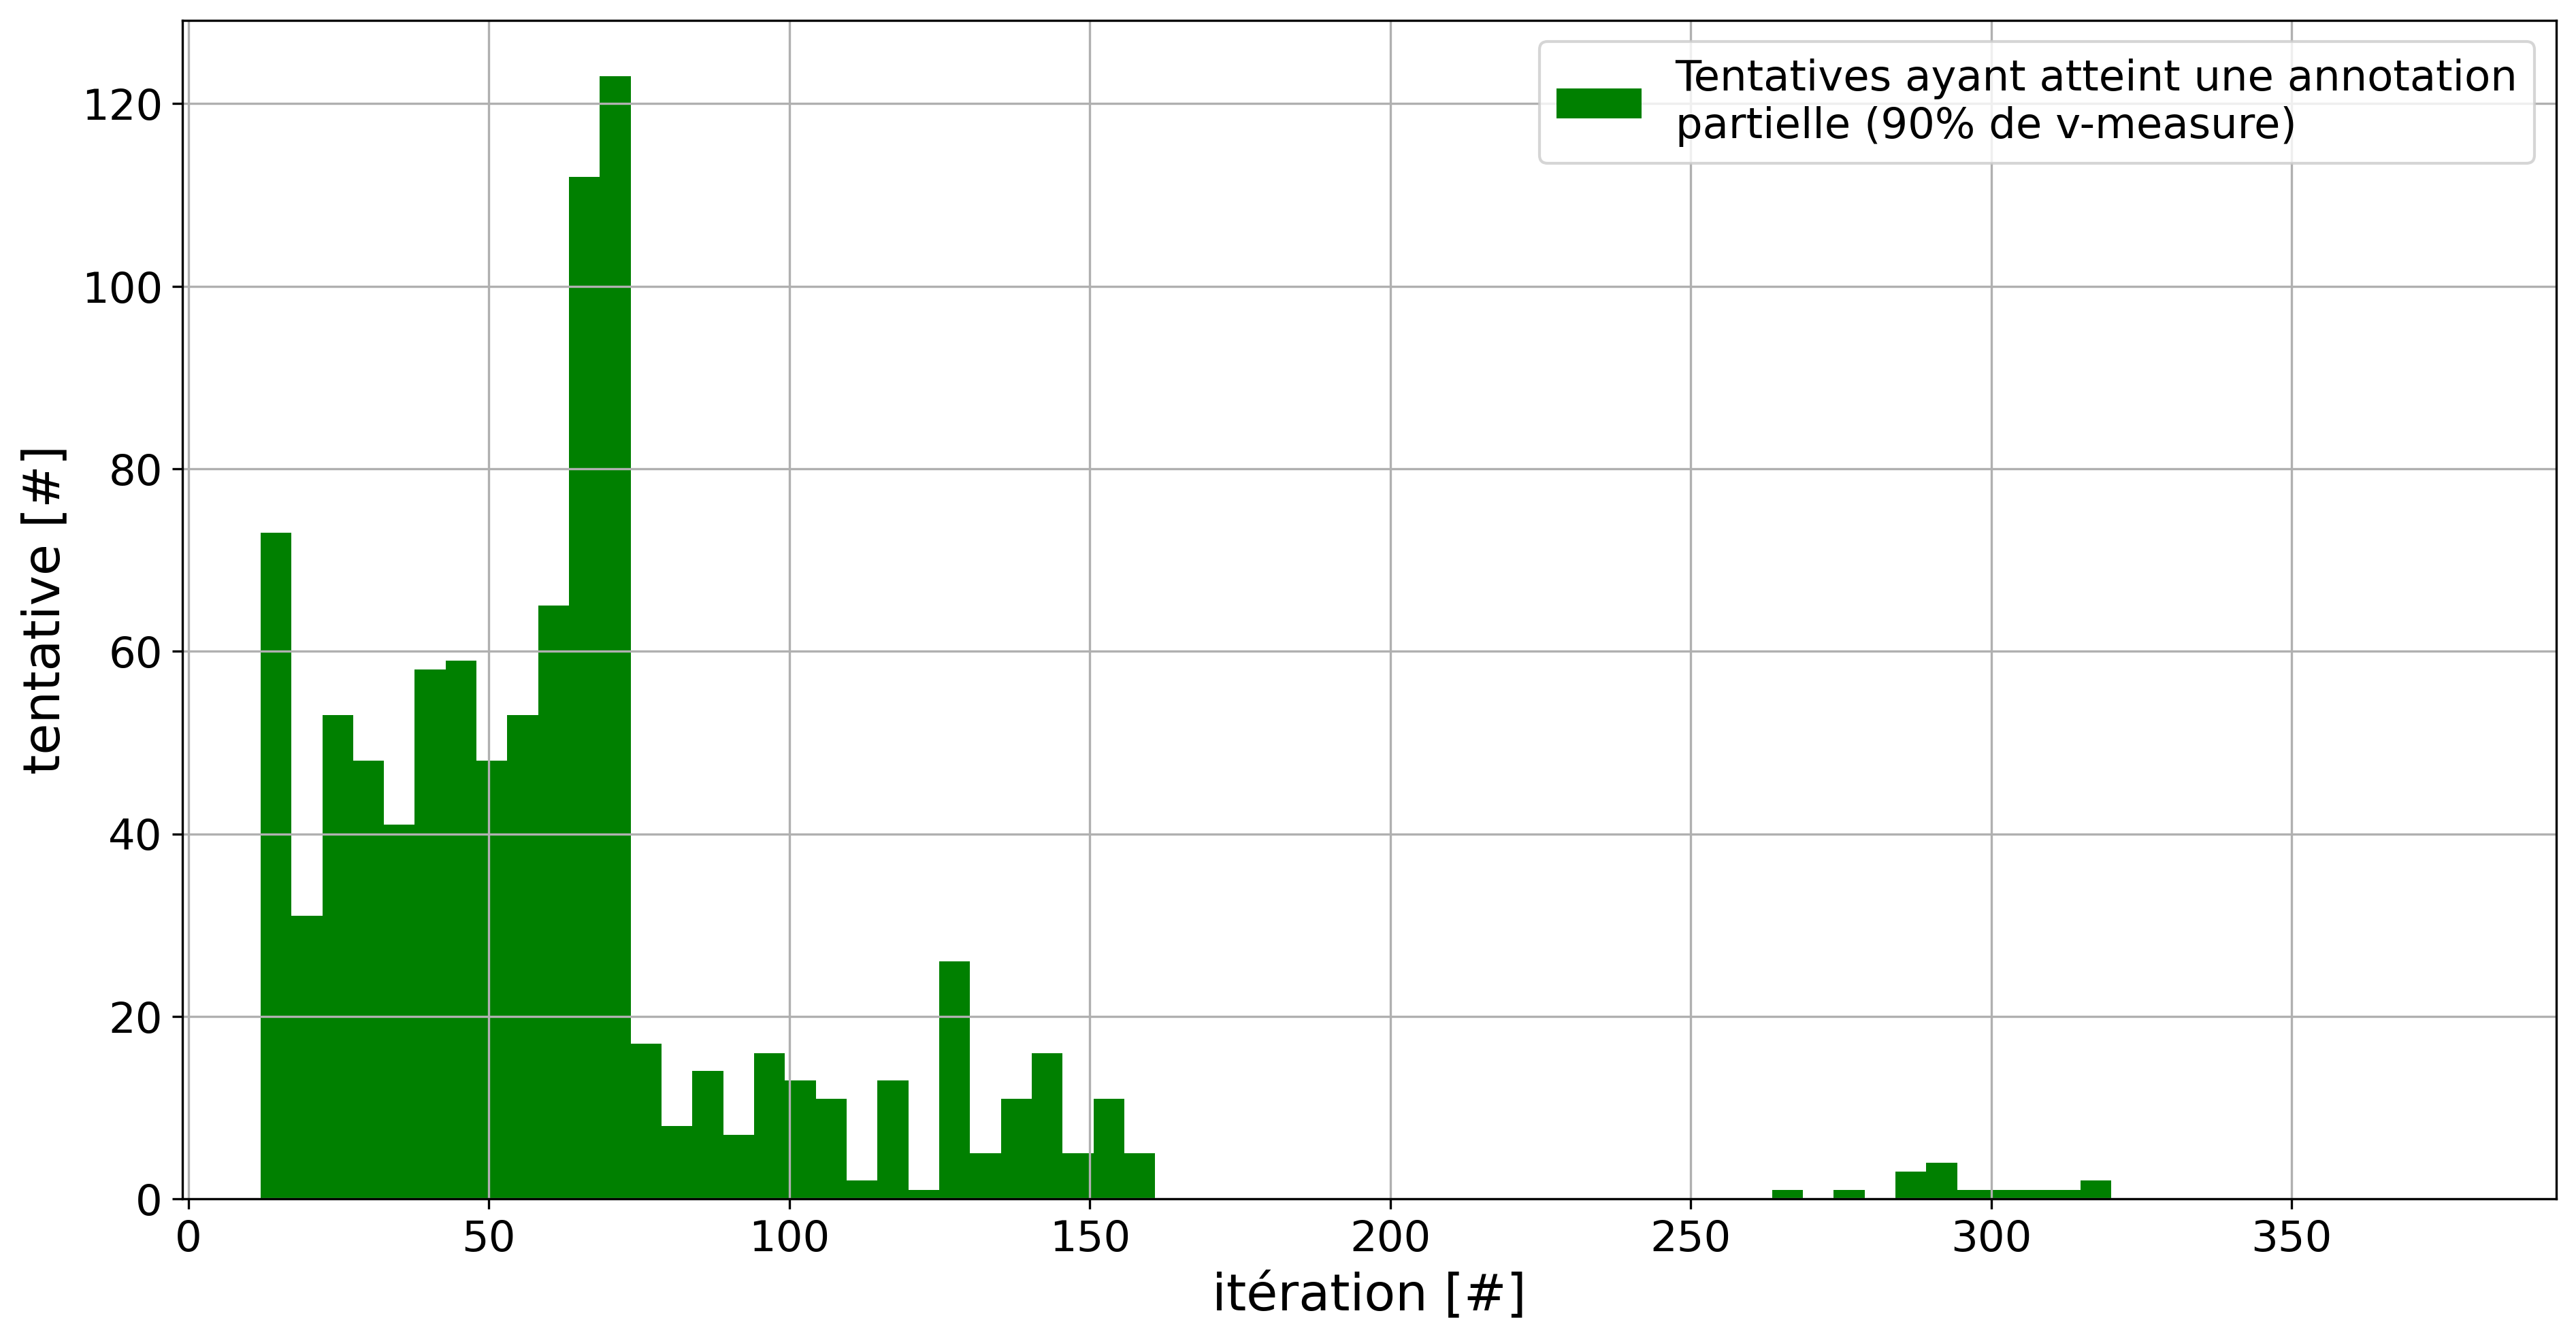
\includegraphics[width=0.95\textwidth]{figures/etude-efficience-histogramme-annotation-partielle}
				\caption{Répartition des tentatives en fonction de l'itération de la méthode à laquelle elles atteignent le seuil d'une annotation partielle, c'est-à-dire l'itération à laquelle elles parviennent à $90$\% de \texttt{v-measure} entre un résultat obtenu et la vérité terrain. L'histogramme est réduit à $60$ pics pour simplifier l'affichage.}
				\label{figure:4.2.1-ETUDE-OPTIMISATION-HISTOGRAMME-ANNOTATION-PARTIELLE}
			\end{figure}
			%
			Le tableau~\ref{table:4.2.1-ETUDE-OPTIMISATION-ANOVA-ANNOTATION-PARTIELLE} retranscrit l'influence de chacun des paramètres sur le nombre d'itérations nécessaires pour atteindre une \textbf{annotation partielle} (\textit{atteindre une \texttt{v-measure} de $90$\%}).
			Les analyses de variance mettent en relief l'effet significatif sur cette convergence du prétraitement (\texttt{eta-carré}: $0.320$, \texttt{p-valeur}: $< 10^{-3}$), de la vectorisation (\texttt{eta-carré}: $0.388$, \texttt{p-valeur}: $< 10^{-3}$), du \textit{clustering} (\texttt{eta-carré}: $0.866$, \texttt{p-valeur}: $< 10^{-3}$) et de l'échantillonnage (\texttt{eta-carré}: $0.968$, \texttt{p-valeur}: $< 10^{-3}$).
			L'analyse post-hoc de ces effets indique que le meilleur paramétrage moyen pour atteindre une \textbf{annotation partielle} repose sur la prétraitement \texttt{prep.simple}, le vectorisation \texttt{vect.tfidf}, le \textit{clustering} \texttt{clust.hier.avg}, et l'échantillonnage \texttt{samp.closest.diff}. La moyenne du nombre d'itération requis pour ce paramétrage est de $19.00$ (écart-type: $0.79$), soit $950$ annotations (écart-type: $39.34$).
			%
			\begin{table}[!htb]
				\begin{center}
				\begin{tabular}{|c|c|c|c|c|c|c|}
					\hline
					% ENTETE DU TABLEAU
					\multicolumn{2}{|c|}{ \shortstack{Description des \\ facteurs analysés } }
						& \multicolumn{3}{c|}{ \shortstack{ Description statistique \\ des itérations } }
						& \multicolumn{2}{c|}{ \shortstack{ Description des \\ tailles d'effets } }
						\tabularnewline
						\hline

					Facteur
						& Niveau 
						& Moyenne
						& Rang
						& SE
						& \texttt{ $ \eta^{2} $ }
						& \texttt{p-valeur}
						\tabularnewline
						\hline
					
					% PRETRAITEMENT
					\multirow{4}{*}{prétraitement}
						& \texttt{prep.simple}
						& $61.90$
						& (1)
						& \multirow{4}{*}{ $0.32$ }
						& \multirow{4}{*}{ $0.320$ }
						& \multirow{4}{*}{ \shortstack{ $< 10^{-3}$ \\ ($***$) } }
						\tabularnewline
						\cline{2-4}
						
						& \texttt{prep.lemma}
						& $63.08$
						& (2)
						&
						&
						&
						\tabularnewline
						\cline{2-4}
						
						& \texttt{prep.no}
						& $63.70$
						& (2)
						&
						& 
						&
						\tabularnewline
						\cline{2-4}
						
						& \texttt{prep.filter}
						& $71.90$
						& (4)
						&
						&
						&
						\tabularnewline
						\hline
					
					% VECTORISATION
					\multirow{2}{*}{vectorisation}
						& \texttt{vect.tfidf}
						& $60.61$
						& (1)
						& \multirow{2}{*}{ $0.29$ }
						& \multirow{2}{*}{ $0.388$ }
						& \multirow{2}{*}{ \shortstack{$< 10^{-3}$ \\ ($***$) } }
						\tabularnewline
						\cline{2-4}
						
						& \texttt{vect.frcorenewsmd}
						& $63.08$
						& (2)
						&
						&
						&
						\tabularnewline
						\hline
					
					% CLUSTERING
					\multirow{6}{*}{clustering}
						& \texttt{clust.hier.avg}
						& $50.64$
						& (1)
						& \multirow{6}{*}{ $0.35$ }
						& \multirow{6}{*}{ $0.866$ }
						& \multirow{6}{*}{ \shortstack{ $< 10^{-3}$ \\ ($***$) } }
						\tabularnewline
						\cline{2-4}
						
						& \texttt{clust.kmeans.cop}
						& $52.43$
						& (2)
						&
						&
						&
						\tabularnewline
						\cline{2-4}
						
						& \texttt{clust.hier.sing}
						& $54.08$
						& (3)
						&
						& 
						&
						\tabularnewline
						\cline{2-4}
						
						& \texttt{clust.hier.ward}
						& $72.41$
						& (4)
						&
						& 
						&
						\tabularnewline
						\cline{2-4}
						
						& \texttt{clust.hier.comp}
						& $73.48$
						& (5)
						&
						&
						&
						\tabularnewline
						\cline{2-4}
						
						& \texttt{clust.spec}
						& $87.84$
						& (6)
						&
						& 
						&
						\tabularnewline
						\hline
					
					% ECHANTILLONNAGE
					\multirow{4}{*}{échantillonnage}
						& \texttt{samp.closest.diff}
						& $33.66$
						& (1)
						& \multirow{4}{*}{ $0.32$ }
						& \multirow{4}{*}{ $0.968$ }
						& \multirow{4}{*}{ \shortstack{ $< 10^{-3}$ \\ ($***$) } }
						\tabularnewline
						\cline{2-4}
						
						& \texttt{samp.random.same}
						& $48.24$
						& (2)
						&
						&
						&
						\tabularnewline
						\cline{2-4}
						
						& \texttt{samp.random.full}
						& $65.83$
						& (3)
						&
						& 
						&
						\tabularnewline
						\cline{2-4}
						
						& \texttt{samp.farhtest.same}
						& $112.86$
						& (4)
						&
						&
						&
						\tabularnewline
						\hline
				\end{tabular}
				\end{center}
				\caption{ANOVA du nombre d'itérations nécessaires pour l'obtention de $90$\% de v-mesure. Les (\textit{$*$}) dénotent le niveau de significativité ($\alpha=0.05$). Pour les effets significatifs, les chiffres précisés entre parenthèses dans la colonne \texttt{Moyenne} indiquent le classement des niveaux selon les analyses post-hoc.}
				\label{table:4.2.1-ETUDE-OPTIMISATION-ANOVA-ANNOTATION-PARTIELLE}
			\end{table}
			

			%%% Analyse d'une annotation suffisante.
			Pour obtenir une \textbf{annotation suffisante} (\textit{atteindre une \texttt{v-measure} de $100$\%}), la moyenne des itérations est de $76.29$ (min: $19$, max: $328$, écart-type: $46.44$), soit une moyenne de $3~801.19$ annotations (min: $950$, max: $16~400$, écart-type: $2~314.91$).
			La figure~\ref{figure:4.2.1-ETUDE-OPTIMISATION-HISTOGRAMME-ANNOTATION-SUFFISANTE} représente la répartition de ces itérations au cours des différentes tentatives.
			On peut noter les deux cas intéressants suivants :
			%
			\begin{itemize}
				\item[$\bullet$] Les tentatives les plus rapides furent celles avec un prétraitement des données \texttt{prep.simple}, une vectorisation des données \texttt{vect.tfidf}, un \textit{clustering} sous contraintes \texttt{clust.hier.comp} ou \texttt{clust.hier.ward}, et un échantillonnage de contraintes \texttt{samp.closest.diff}. Ces tentatives ont requis $19$ itérations, soit $950$ annotations, dont $638$ (respectivement $641$) contraintes \texttt{MUST-LINK}.
				\item[$\bullet$] Les tentatives les plus lentes furent celles avec un prétraitement des données \texttt{prep.no}, une vectorisation des données \texttt{vect.tfidf}, un \textit{clustering} sous contraintes \texttt{clust.spec}, et un échantillonnage de contraintes \texttt{samp.farthest.same}. Ces tentatives ont requis $394$ itérations, soit $16~400$ annotations, dont $1~309$ contraintes \texttt{MUST-LINK}.
			\end{itemize}
			%
			\begin{figure}[!htb]
				\centering
				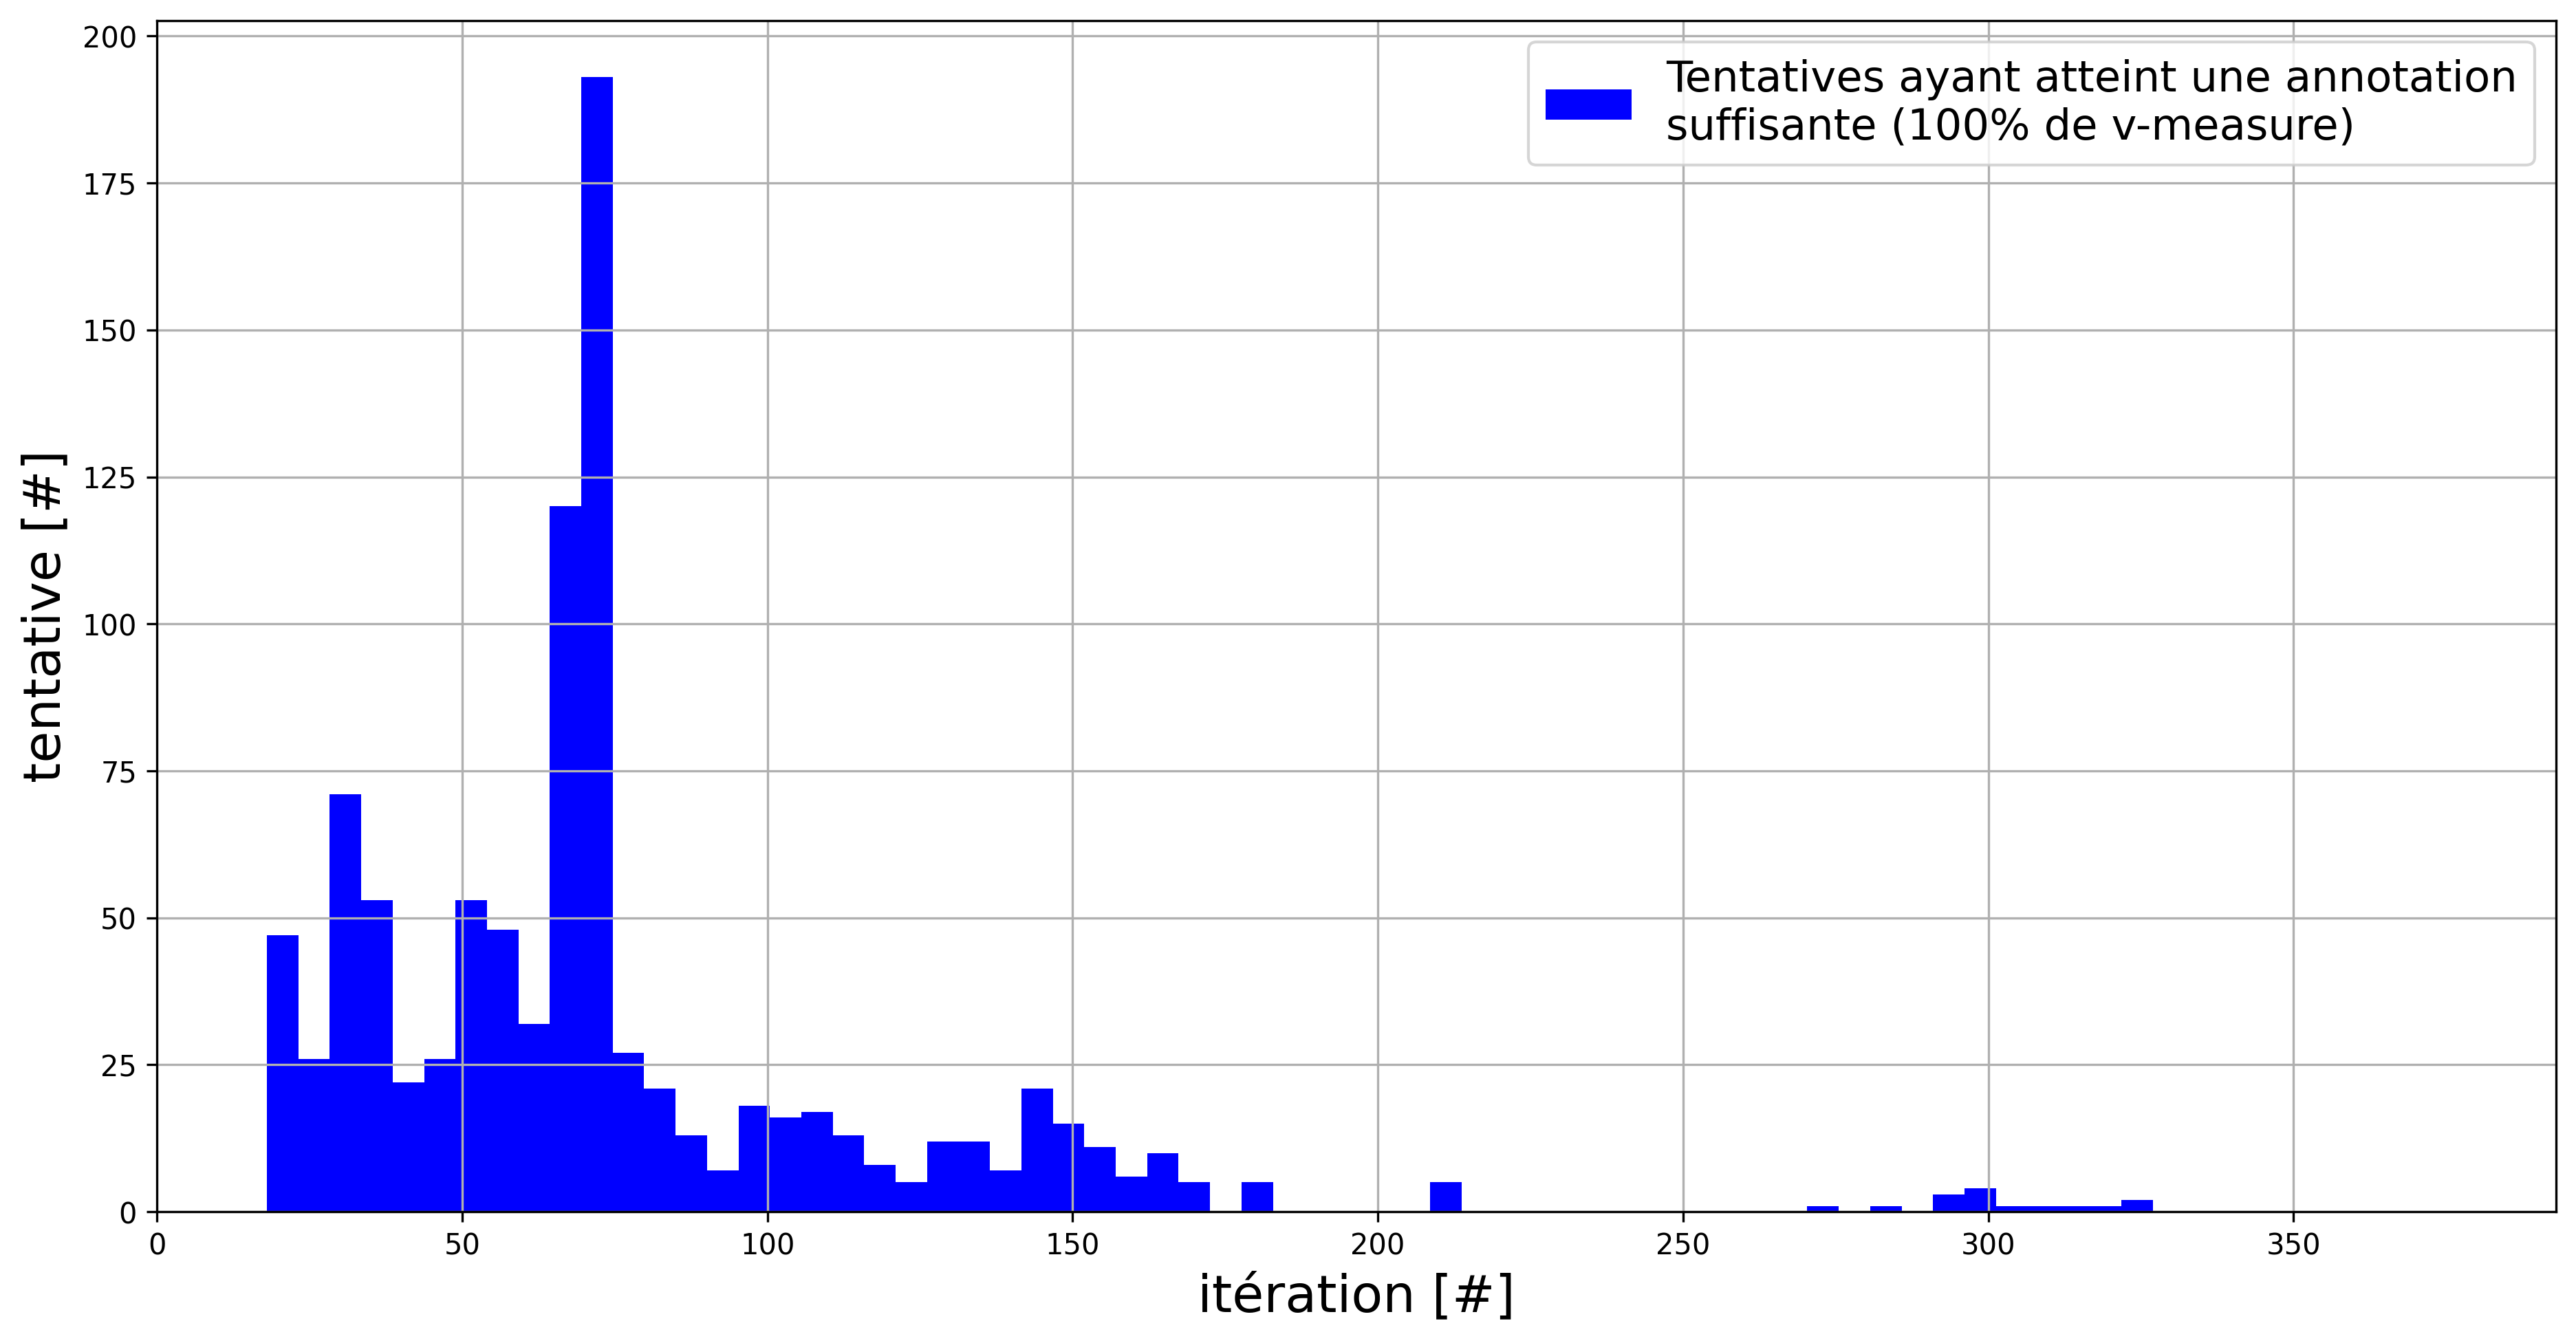
\includegraphics[width=0.95\textwidth]{figures/etude-efficience-histogramme-annotation-suffisante}
				\caption{Répartition des tentatives en fonction de l'itération de la méthode à laquelle elles atteignent le seuil d'une annotation suffisante, c'est-à-dire l'itération à laquelle elles parviennent à $100$\% de \texttt{v-measure} entre un résultat obtenu et la vérité terrain. L'histogramme est réduit à $60$ pics pour simplifier l'affichage.}
				\label{figure:4.2.1-ETUDE-OPTIMISATION-HISTOGRAMME-ANNOTATION-SUFFISANTE}
			\end{figure}
			%
			Le tableau~\ref{table:4.2.1-ETUDE-OPTIMISATION-ANOVA-ANNOTATION-SUFFISANTE} retranscrit l'influence de chacun des paramètres sur le nombre d'itérations nécessaires pour atteindre une \textbf{annotation suffisante}.
			Les analyses de variance mettent en relief l'effet significatif sur cette convergence du prétraitement (\texttt{eta-carré}: $0.987$, \texttt{p-valeur}: $< 10^{-3}$), de la vectorisation (\texttt{eta-carré}: $0.991$, \texttt{p-valeur}: $< 10^{-3}$), du \textit{clustering} (\texttt{eta-carré}: $0.997$, \texttt{p-valeur}: $< 10^{-3}$) et de l'échantillonnage (\texttt{eta-carré}: $0.998$, \texttt{p-valeur}: $< 10^{-3}$).
			L'analyse post-hoc de ces effets indique que le meilleur paramétrage moyen pour atteindre une \textbf{annotation suffisante} repose sur la prétraitement \texttt{prep.lemma}, le vectorisation \texttt{vect.tfidf}, le \textit{clustering} \texttt{clust.kmeans.cop}, et l'échantillonnage \texttt{samp.closest.diff}. La moyenne du nombre d'itération requis pour ce paramétrage est de $34.60$ (écart-type: $7.44$), soit $1~730$ annotations (écart-type: $372.00$).
			%
			\begin{table}[!htb]
				\begin{center}
				\begin{tabular}{|c|c|c|c|c|c|c|}
					\hline
					% ENTETE DU TABLEAU
					\multicolumn{2}{|c|}{ \shortstack{Description des \\ facteurs analysés } }
						& \multicolumn{3}{c|}{ \shortstack{ Description statistique \\ des itérations } }
						& \multicolumn{2}{c|}{ \shortstack{ Description des \\ tailles d'effets } }
						\tabularnewline
						\hline

					Facteur
						& Niveau 
						& Moyenne
						& Rang
						& SE
						& \texttt{ $\eta^{2}$ }
						& \texttt{p-valeur}
						\tabularnewline
						\hline
					
					% PRETRAITEMENT
					\multirow{4}{*}{prétraitement}
						& \texttt{prep.lemma}
						& $72.86$
						& (1)
						& \multirow{4}{*}{ $0.32$ }
						& \multirow{4}{*}{ $0.276$ }
						& \multirow{4}{*}{ \shortstack{ $< 10^{-3}$ \\ ($***$) } }
						\tabularnewline
						\cline{2-4}
						
						& \texttt{prep.simple}
						& $73.30$
						& (2)
						&
						&
						&
						\tabularnewline
						\cline{2-4}
						
						& \texttt{prep.no}
						& $75.24$
						& (2)
						&
						& 
						&
						\tabularnewline
						\cline{2-4}
						
						& \texttt{prep.filter}
						& $83.77$
						& (4)
						&
						&
						&
						\tabularnewline
						\hline
					
					% VECTORISATION
					\multirow{2}{*}{vectorisation}
						& \texttt{vect.tfidf}
						& $71.16$
						& (1)
						& \multirow{2}{*}{ $0.36$ }
						& \multirow{2}{*}{ $0.366$ }
						& \multirow{2}{*}{ \shortstack{$< 10^{-3}$ \\ ($***$)} }
						\tabularnewline
						\cline{2-4}
						
						& \texttt{vect.frcorenewsmd}
						& $81.43$
						& (2)
						&
						&
						&
						\tabularnewline
						\hline
					
					% CLUSTERING
					\multirow{6}{*}{clustering}
						& \texttt{clust.kmeans.cop}
						& $62.23$
						& (1)
						& \multirow{6}{*}{ $0.42$ }
						& \multirow{6}{*}{ $0.700$ }
						& \multirow{6}{*}{ \shortstack{$< 10^{-3}$ \\ ($***$)} }
						\tabularnewline
						\cline{2-4}
						
						& \texttt{clust.hier.avg}
						& $65.13$
						& (2)
						&
						&
						&
						\tabularnewline
						\cline{2-4}
						
						& \texttt{clust.hier.sing}
						& $75.44$
						& (3)
						&
						& 
						&
						\tabularnewline
						\cline{2-4}
						
						& \texttt{clust.hier.ward}
						& $80.44$
						& (4)
						&
						& 
						&
						\tabularnewline
						\cline{2-4}
						
						& \texttt{clust.hier.comp}
						& $81.46$
						& (5)
						&
						&
						&
						\tabularnewline
						\cline{2-4}
						
						& \texttt{clust.spec}
						& $93.06$
						& (6)
						&
						& 
						&
						\tabularnewline
						\hline
					
					% ECHANTILLONNAGE
					\multirow{4}{*}{échantillonnage}
						& \texttt{samp.closest.diff}
						& $50.29$
						& (1)
						& \multirow{4}{*}{ $0.39$ }
						& \multirow{4}{*}{ $0.950$ }
						& \multirow{4}{*}{ \shortstack{$< 10^{-3}$ \\ ($***$)} }
						\tabularnewline
						\cline{2-4}
						
						& \texttt{samp.random.same}
						& $56.38$
						& (2)
						&
						&
						&
						\tabularnewline
						\cline{2-4}
						
						& \texttt{samp.random.full}
						& $71.95$
						& (3)
						&
						& 
						&
						\tabularnewline
						\cline{2-4}
						
						& \texttt{samp.farhtest.same}
						& $126.55$
						& (4)
						&
						&
						&
						\tabularnewline
						\hline
				\end{tabular}
				\end{center}
				\caption{ANOVA du nombre d'itérations nécessaires pour l'obtention de $100$\% de v-mesure. Les (\textit{$*$}) dénotent le niveau de significativité ($\alpha=0.05$). Pour les effets significatifs, les chiffres précisés entre parenthèses dans la colonne \texttt{Moyenne} indiquent le classement des niveaux selon les analyses post-hoc.}
				\label{table:4.2.1-ETUDE-OPTIMISATION-ANOVA-ANNOTATION-SUFFISANTE}
			\end{table}
			
			%%% Analyse d'une annotation exhaustive.
			Enfin, pour avoir une \textbf{annotation exhaustive} (\textit{annoter toutes les contraintes possibles}), la moyenne des itérations est de $88.98$ (min: $20$, max: $394$, écart-type: $68.21$), soit une moyenne de $4~431.34$ annotations (min: $1~000$, max: $19~656$, écart-type: $3~405.16$).
			La figure~\ref{figure:4.2.1-ETUDE-OPTIMISATION-HISTOGRAMME-ANNOTATION-EXHAUSTIVE} représente la répartition de ces itérations au cours des différentes tentatives.
			On peut noter les deux cas intéressants suivant :
			%
			\begin{itemize}
				\item[$\bullet$] Les tentatives les plus rapides furent celles avec un prétraitement des données \texttt{prep.no} ou \texttt{prep.lemma}, une vectorisation des données \texttt{vect.tfidf}, un algorithme de \textit{clustering} sous contraintes \texttt{clust.hier.comp} ou \texttt{clust.hier.ward}, et un échantillonnage de contraintes \texttt{samp.closest.diff}. Ces tentatives ont requis $20$ itérations, soit $1~000$ annotations, dont $653$ (respectivement $668$) contraintes \texttt{MUST-LINK}.
				\item[$\bullet$] Les tentatives les plus lentes furent celles avec un prétraitement des données \texttt{prep.simple}, une vectorisation des données \texttt{vect.frcorenewsmd}, un \textit{clustering} \texttt{clust.hier.sing}, et un échantillonnage de contraintes \texttt{samp.closest.diff}. Ces tentatives ont requis $394$ itérations, soit $19~656$ annotations, dont $682$ contraintes \texttt{MUST-LINK}.
			\end{itemize}
			%
			\begin{figure}[!htb]
				\centering
				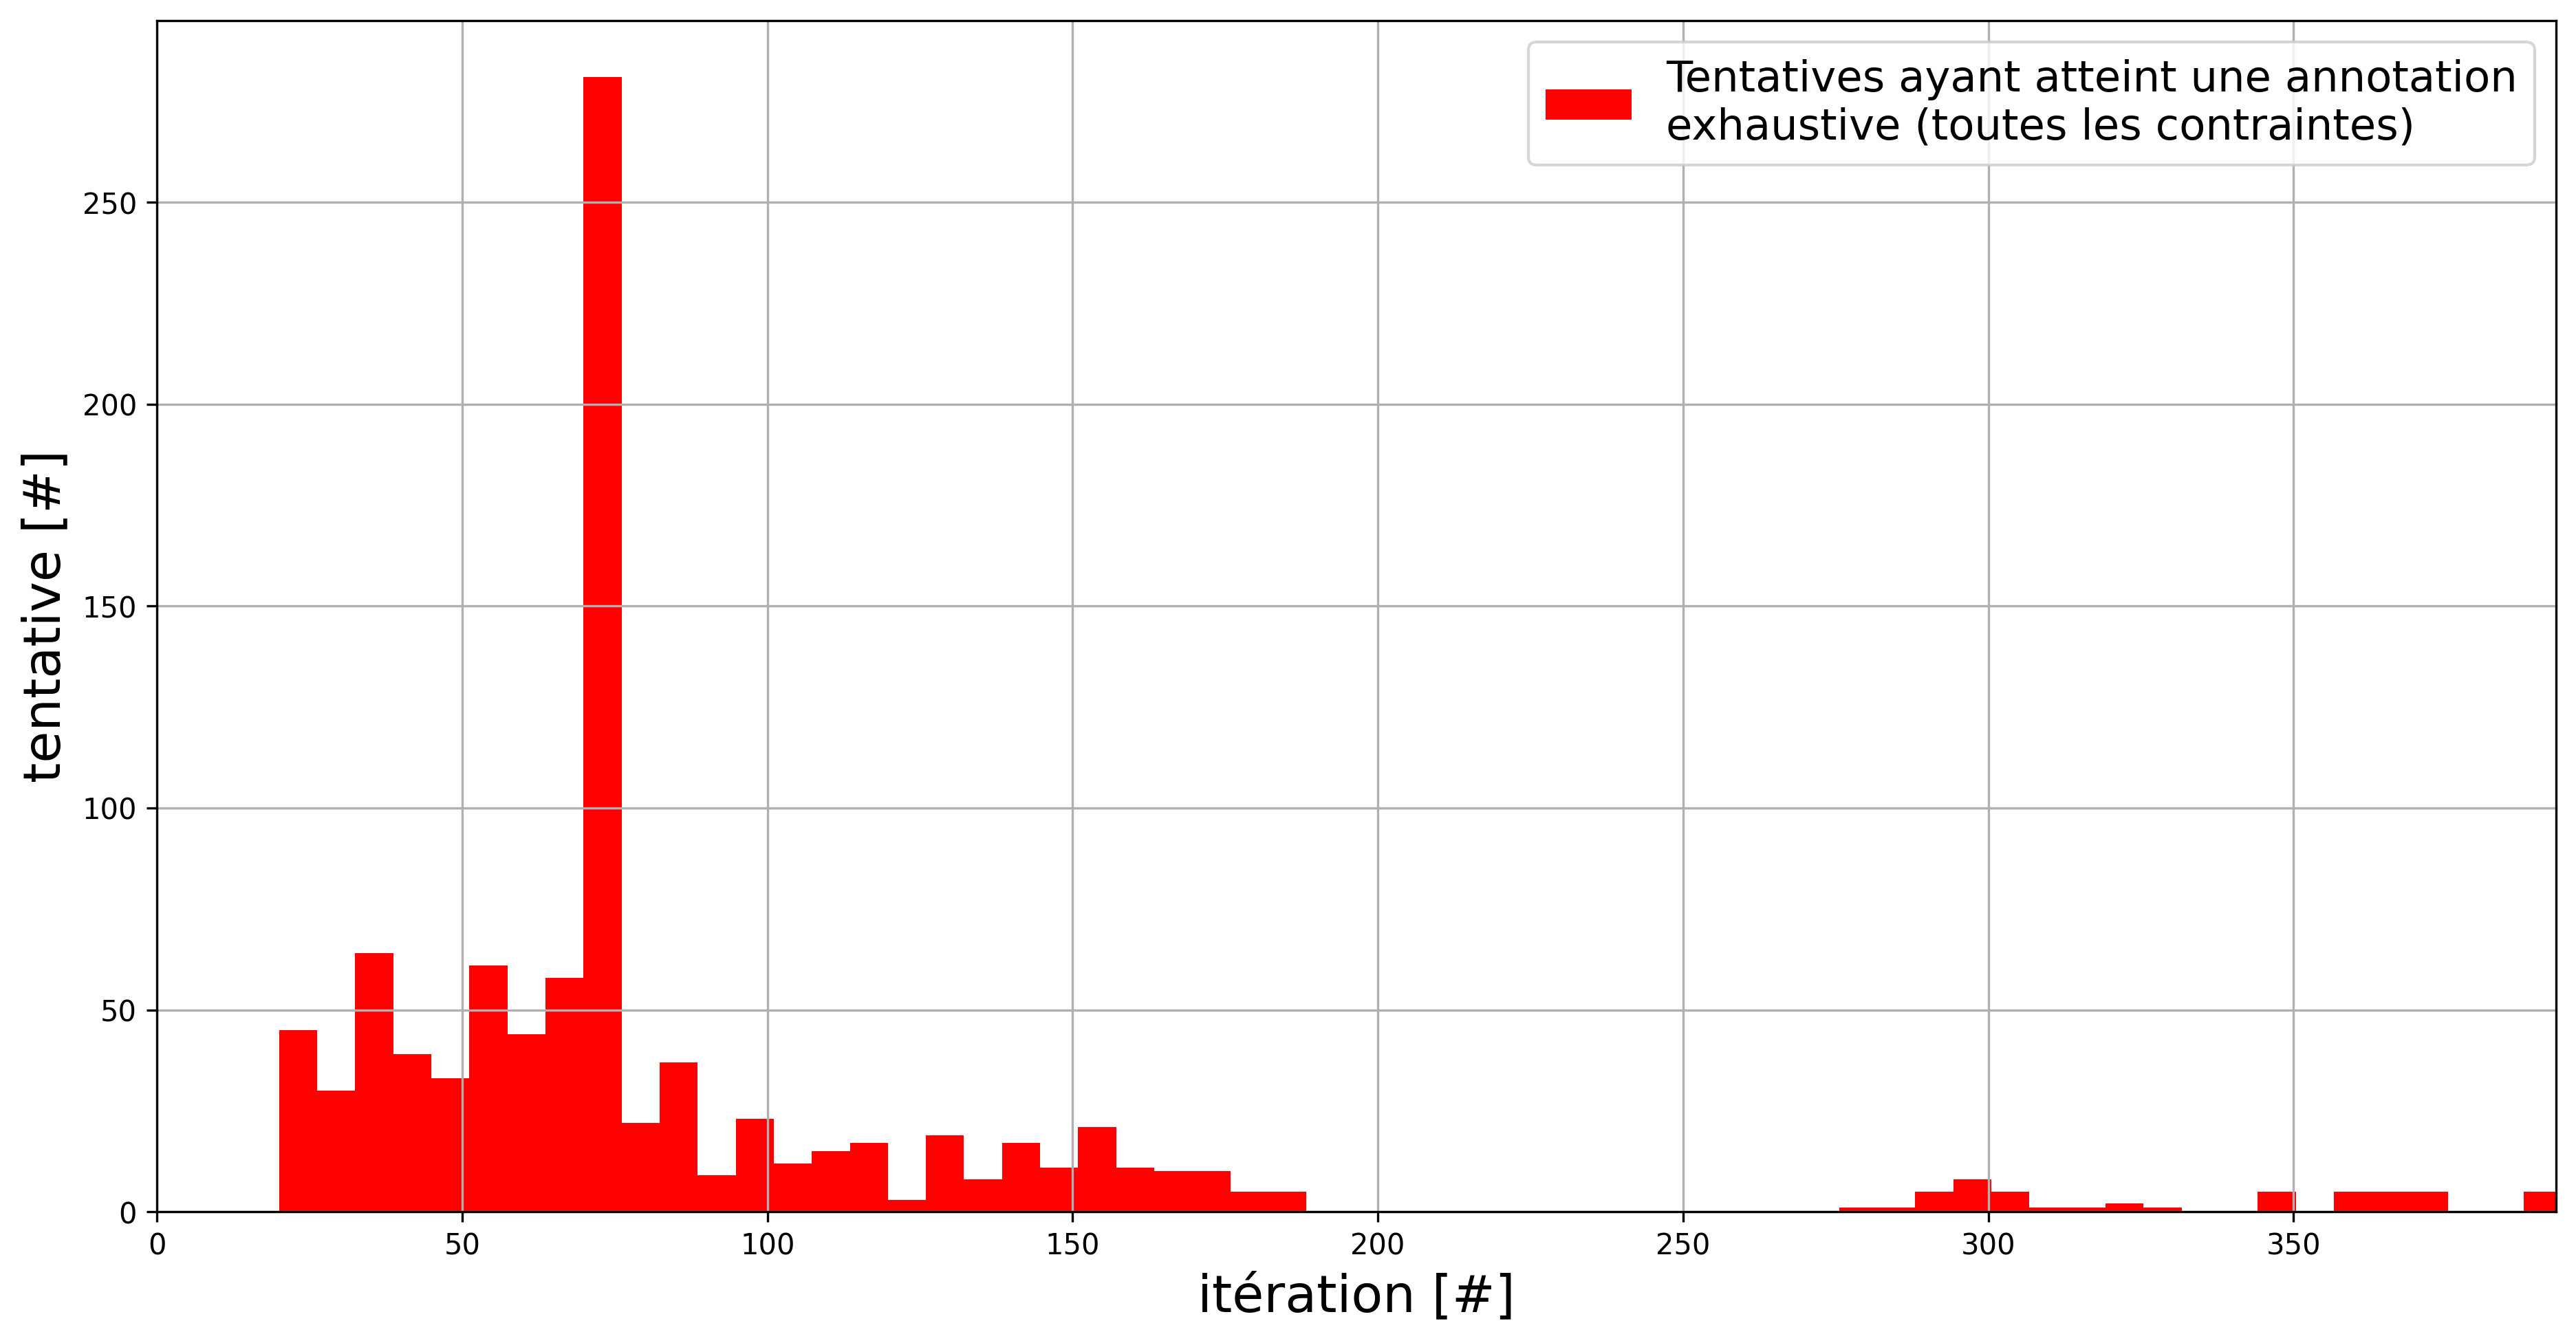
\includegraphics[width=0.95\textwidth]{figures/etude-efficience-histogramme-annotation-exhaustive}
				\caption{Répartition des tentatives en fonction de l'itération de la méthode à laquelle elles atteignent le seuil d'une annotation exhaustive, c'est-à-dire l'itération à laquelle toutes les contraintes possibles entre les données ont été annotées. L'histogramme est réduit à $60$ pics pour simplifier l'affichage.}
				\label{figure:4.2.1-ETUDE-OPTIMISATION-HISTOGRAMME-ANNOTATION-EXHAUSTIVE}
			\end{figure}
			%
			Le tableau~\ref{table:4.2.1-ETUDE-OPTIMISATION-ANOVA-ANNOTATION-EXHAUSTIVE} retranscrit l'influence de chacun des paramètres sur le nombre d'itérations nécessaires pour atteindre une \textbf{annotation exhaustive}.
			Les analyses de variance mettent en relief l'effet significatif sur cette convergence du prétraitement (\texttt{eta-carré}: $0.909$, \texttt{p-valeur}: $< 10^{-3}$), de la vectorisation (\texttt{eta-carré}: $0.985$, \texttt{p-valeur}: $< 10^{-3}$), du \textit{clustering} (\texttt{eta-carré}: $0.999$, \texttt{p-valeur}: $< 10^{-3}$) et de l'échantillonnage (\texttt{eta-carré}: $0.997$, \texttt{p-valeur}: $< 10^{-3}$).
			L'analyse post-hoc de ces effets indique que le meilleur paramétrage moyen pour atteindre une \textbf{annotation exhaustive} repose sur la prétraitement \texttt{prep.lemma}, le vectorisation \texttt{vect.tfidf}, le \textit{clustering} \texttt{clust.kmeans.cop}, et l'échantillonnage \texttt{samp.random.same}. La moyenne du nombre d'itération requis pour ce paramétrage est de $32.60$ (écart-type: $1.14$), soit $1~630$ annotations (écart-type: $57.00$).
			%
			\begin{table}[!htb]
				\begin{center}
				\begin{tabular}{|c|c|c|c|c|c|c|}
					\hline
					% ENTETE DU TABLEAU
					\multicolumn{2}{|c|}{ \shortstack{Description des \\ facteurs analysés } }
						& \multicolumn{3}{c|}{ \shortstack{ Description statistique \\ des itérations } }
						& \multicolumn{2}{c|}{ \shortstack{ Description des \\ tailles d'effets } }
						\tabularnewline
						\hline

					Facteur
						& Niveau 
						& Moyenne
						& Rang
						& SE
						& \texttt{ $\eta^{2}$ }
						& \texttt{p-valeur}
						\tabularnewline
						\hline
					
					% PRETRAITEMENT
					\multirow{4}{*}{prétraitement}
						& \texttt{prep.lemma}
						& $85.89$
						& (1)
						& \multirow{4}{*}{ $0.42$ }
						& \multirow{4}{*}{ $0.052$ }
						& \multirow{4}{*}{ \shortstack{$< 10^{-3}$ \\ ($***$)} }
						\tabularnewline
						\cline{2-4}
						
						& \texttt{prep.filter}
						& $89.55$
						& (2)
						&
						&
						&
						\tabularnewline
						\cline{2-4}
						
						& \texttt{prep.simple}
						& $89.64$
						& (2)
						&
						& 
						&
						\tabularnewline
						\cline{2-4}
						
						& \texttt{prep.no}
						& $90.81$
						& (4)
						&
						&
						&
						\tabularnewline
						\hline
					
					% VECTORISATION
					\multirow{2}{*}{vectorisation}
						& \texttt{vect.tfidf}
						& $85.50$
						& (1)
						& \multirow{2}{*}{ $0.39$ }
						& \multirow{2}{*}{ $0.165$ }
						& \multirow{2}{*}{ \shortstack{$< 10^{-3}$ \\ ($***$)} }
						\tabularnewline
						\cline{2-4}
						
						& \texttt{vect.frcorenewsmd}
						& $92.46$
						& (2)
						&
						&
						&
						\tabularnewline
						\hline
					
					% CLUSTERING
					\multirow{6}{*}{clustering}
						& \texttt{clust.kmeans.cop}
						& $64.99$
						& (1)
						& \multirow{6}{*}{ $0.39$ }
						& \multirow{6}{*}{ $0.894$ }
						& \multirow{6}{*}{ \shortstack{$< 10^{-3}$ \\ ($***$)} }
						\tabularnewline
						\cline{2-4}
						
						& \texttt{clust.hier.avg}
						& $78.54$
						& (2)
						&
						&
						&
						\tabularnewline
						\cline{2-4}
						
						& \texttt{clust.hier.ward}
						& $81.31$
						& (3)
						&
						& 
						&
						\tabularnewline
						\cline{2-4}
						
						& \texttt{clust.hier.comp}
						& $82.49$
						& (3)
						&
						& 
						&
						\tabularnewline
						\cline{2-4}
						
						& \texttt{clust.spec}
						& $93.78$
						& (5)
						&
						&
						&
						\tabularnewline
						\cline{2-4}
						
						& \texttt{clust.hier.comp}
						& $132.75$
						& (6)
						&
						& 
						&
						\tabularnewline
						\hline
					
					% ECHANTILLONNAGE
					\multirow{4}{*}{échantillonnage}
						& \texttt{samp.random.same}
						& $57.23$
						& (1)
						& \multirow{4}{*}{ $0.42$ }
						& \multirow{4}{*}{ $0.930$ }
						& \multirow{4}{*}{ \shortstack{$< 10^{-3}$ \\ ($***$)} }
						\tabularnewline
						\cline{2-4}
						
						& \texttt{samp.random.full}
						& $72.80$
						& (2)
						&
						&
						&
						\tabularnewline
						\cline{2-4}
						
						& \texttt{samp.closest.diff}
						& $98.38$
						& (3)
						&
						& 
						&
						\tabularnewline
						\cline{2-4}
						
						& \texttt{samp.farhtest.same}
						& $132.75$
						& (4)
						&
						&
						&
						\tabularnewline
						\hline
				\end{tabular}
				\end{center}
				\caption{ANOVA du nombre d'itérations nécessaires pour annoter toutes les contraintes possibles. Les (\textit{$*$}) dénotent le niveau de significativité ($\alpha=0.05$). Pour les effets significatifs, les chiffres précisés entre parenthèses dans la colonne \texttt{Moyenne} indiquent le classement des niveaux selon les analyses post-hoc.}
				\label{table:4.2.1-ETUDE-OPTIMISATION-ANOVA-ANNOTATION-EXHAUSTIVE}
			\end{table}
		
		
			% Graphe d'évolution de la v-measure moyenne, min et max.
			La figure~\ref{figure:4.2.1-ETUDE-OPTIMISATION-EVOLUTION-PAR-FACTEURS} représente les évolutions moyennes de la \texttt{v-measure} du \textit{clustering} en fonction du nombre d'itération de la méthode pour les différentes valeurs des facteurs analysés (prétraitement en haut à gauche, vectorisation en haut à droite, \textit{clustering} en bas à gauche, échantillonnage en bas à droite).
			La figure~\ref{figure:4.2.1-ETUDE-OPTIMISATION-EVOLUTION-MEILLEUR-PARAMETRAGE} représente cette même évolution pour les meilleurs paramétrages moyens destinés à atteindre les trois seuils d'annotation définis (partiel, suffisant, exhaustif).
			%
			\begin{figure}[!htb]
				\centering
				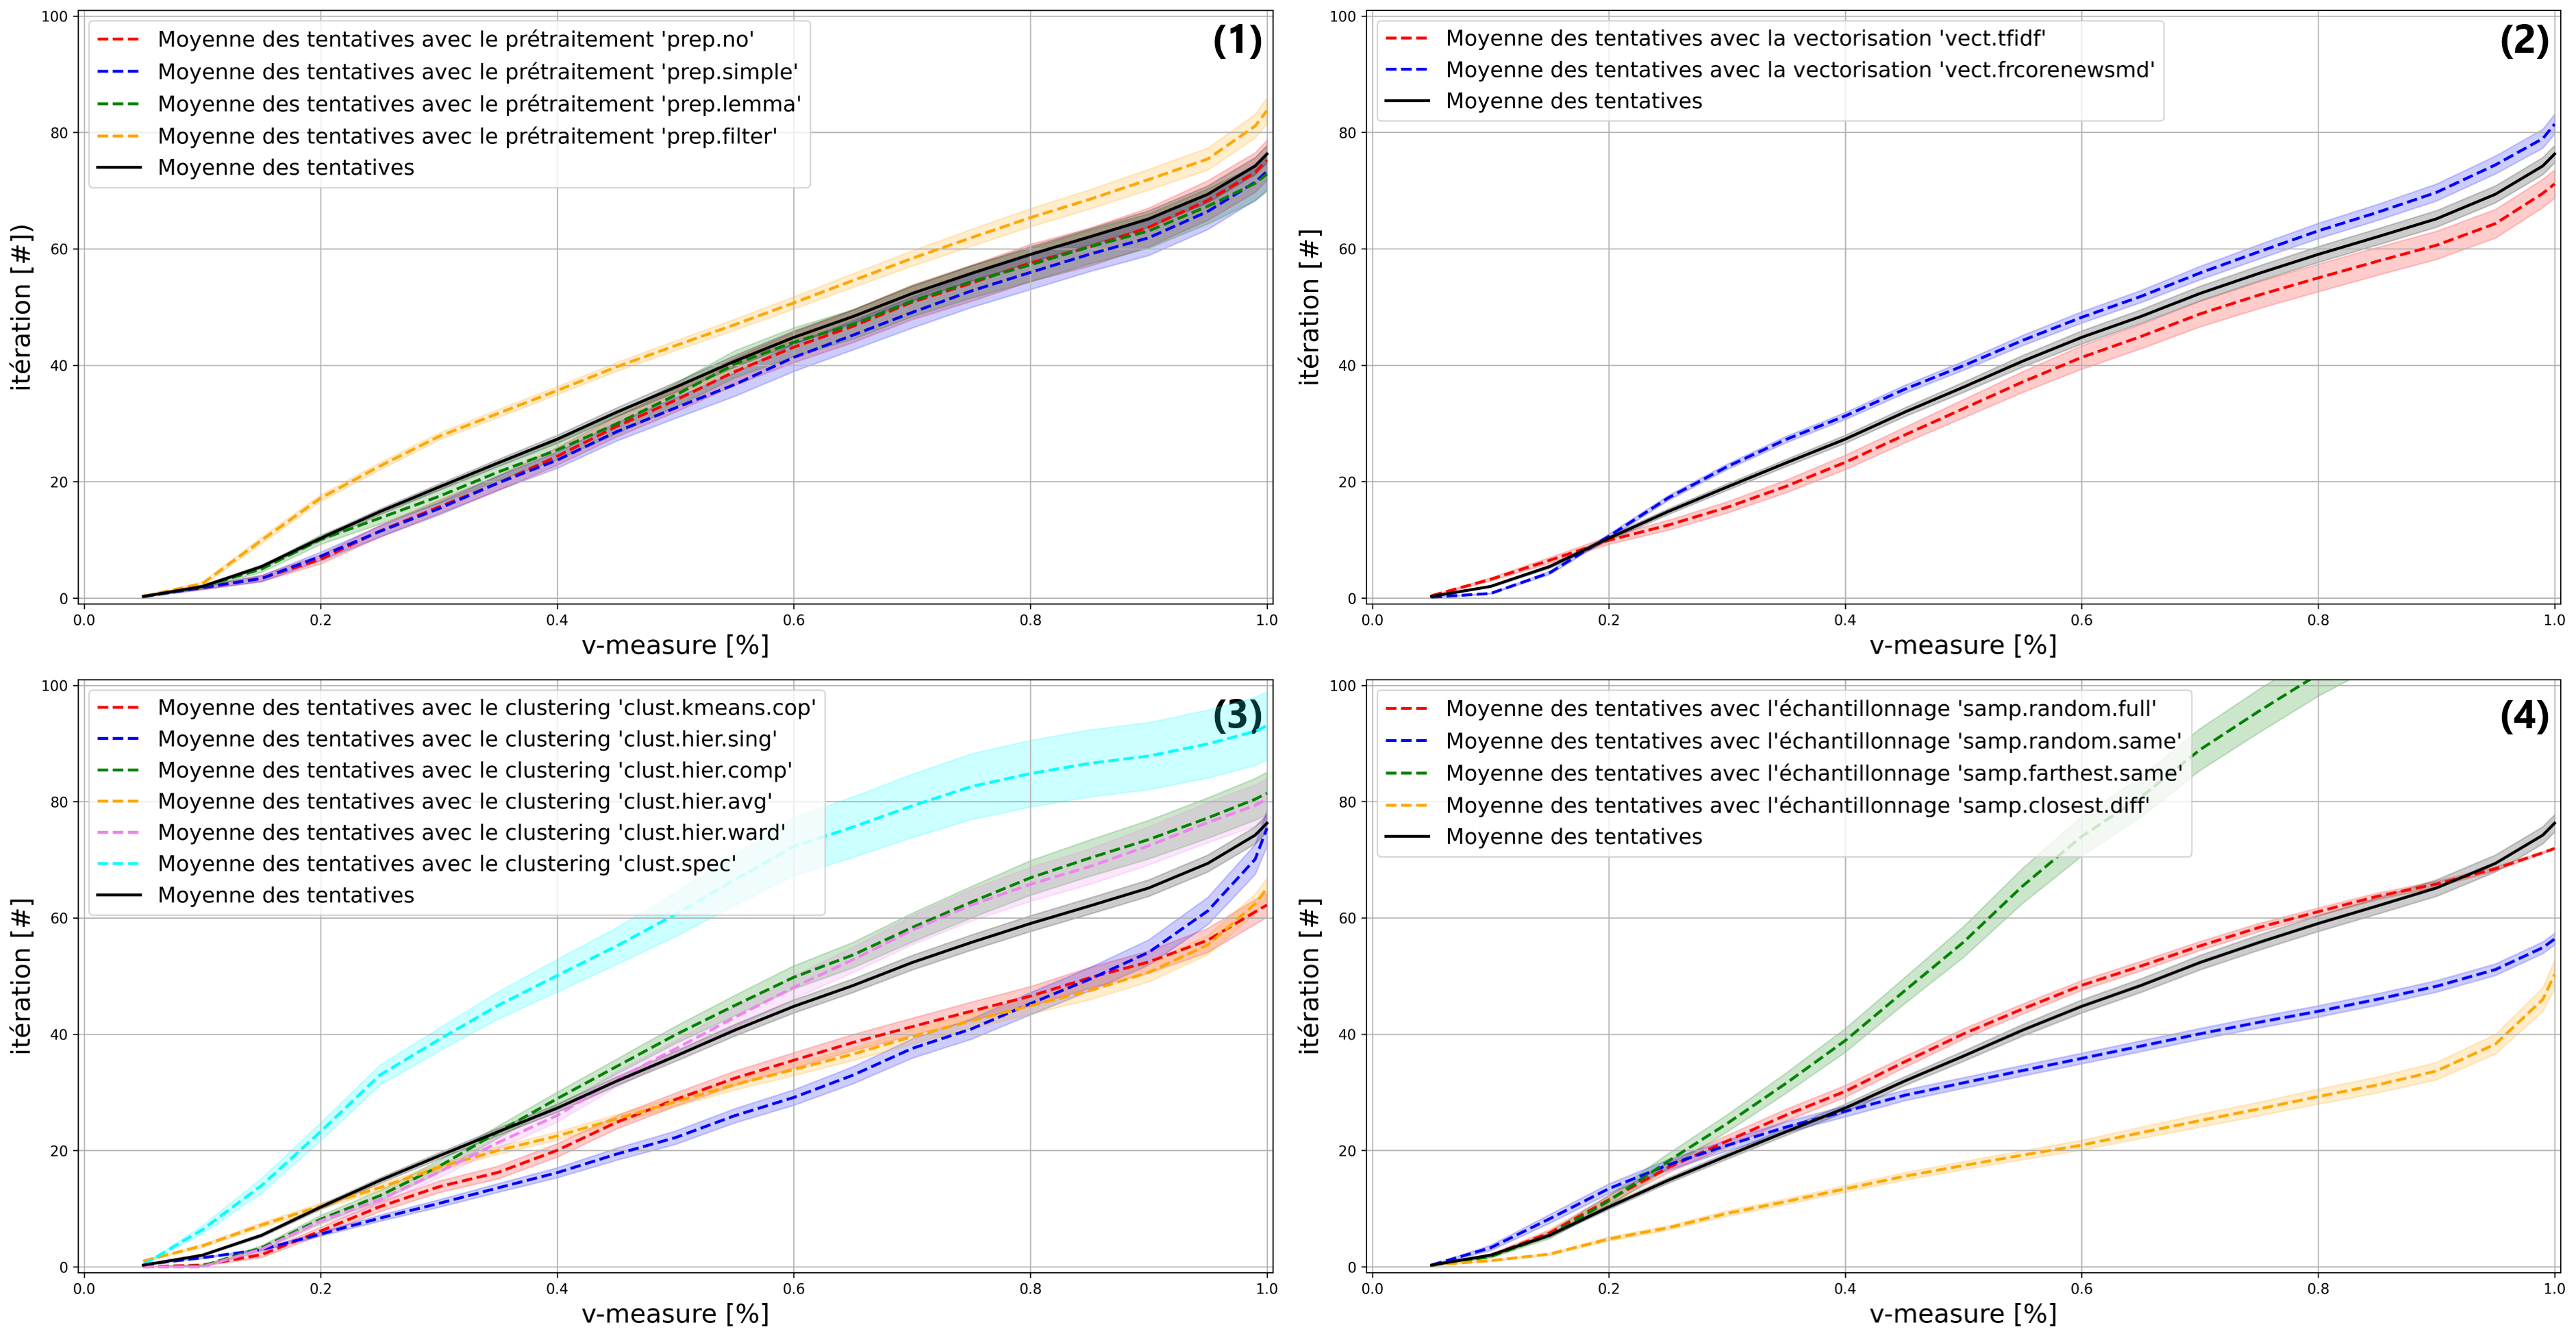
\includegraphics[width=0.95\textwidth]{figures/etude-efficience-evolution-moyenne-par-vmeasure-par-facteur}
				\caption{Évolution des moyennes du nombre d'itérations nécessaire de la méthode de \textit{clustering} interactif pour obtenir un seuil défini de \texttt{v-measure} entre un résultat obtenu et la vérité terrain, moyennes réalisées sur les différentes valeurs que peuvent prendre les facteurs analysés et affichées par facteur : \textbf{(1)} prétraitement, \textbf{(2)} vectorisation, \textbf{(3)} \textit{clustering} et \textbf{(4)} échantillonnage. \\
				Note : \textit{Le seuil d'annotation exhaustive (annoter toutes les contraintes possibles) n'étant pas exprimé en terme de \texttt{v-measure}, ce seuil n'est pas affiché ici.}}
				\label{figure:4.2.1-ETUDE-OPTIMISATION-EVOLUTION-PAR-FACTEURS}
			\end{figure}
			%
			\begin{figure}[!htb]
				\centering
				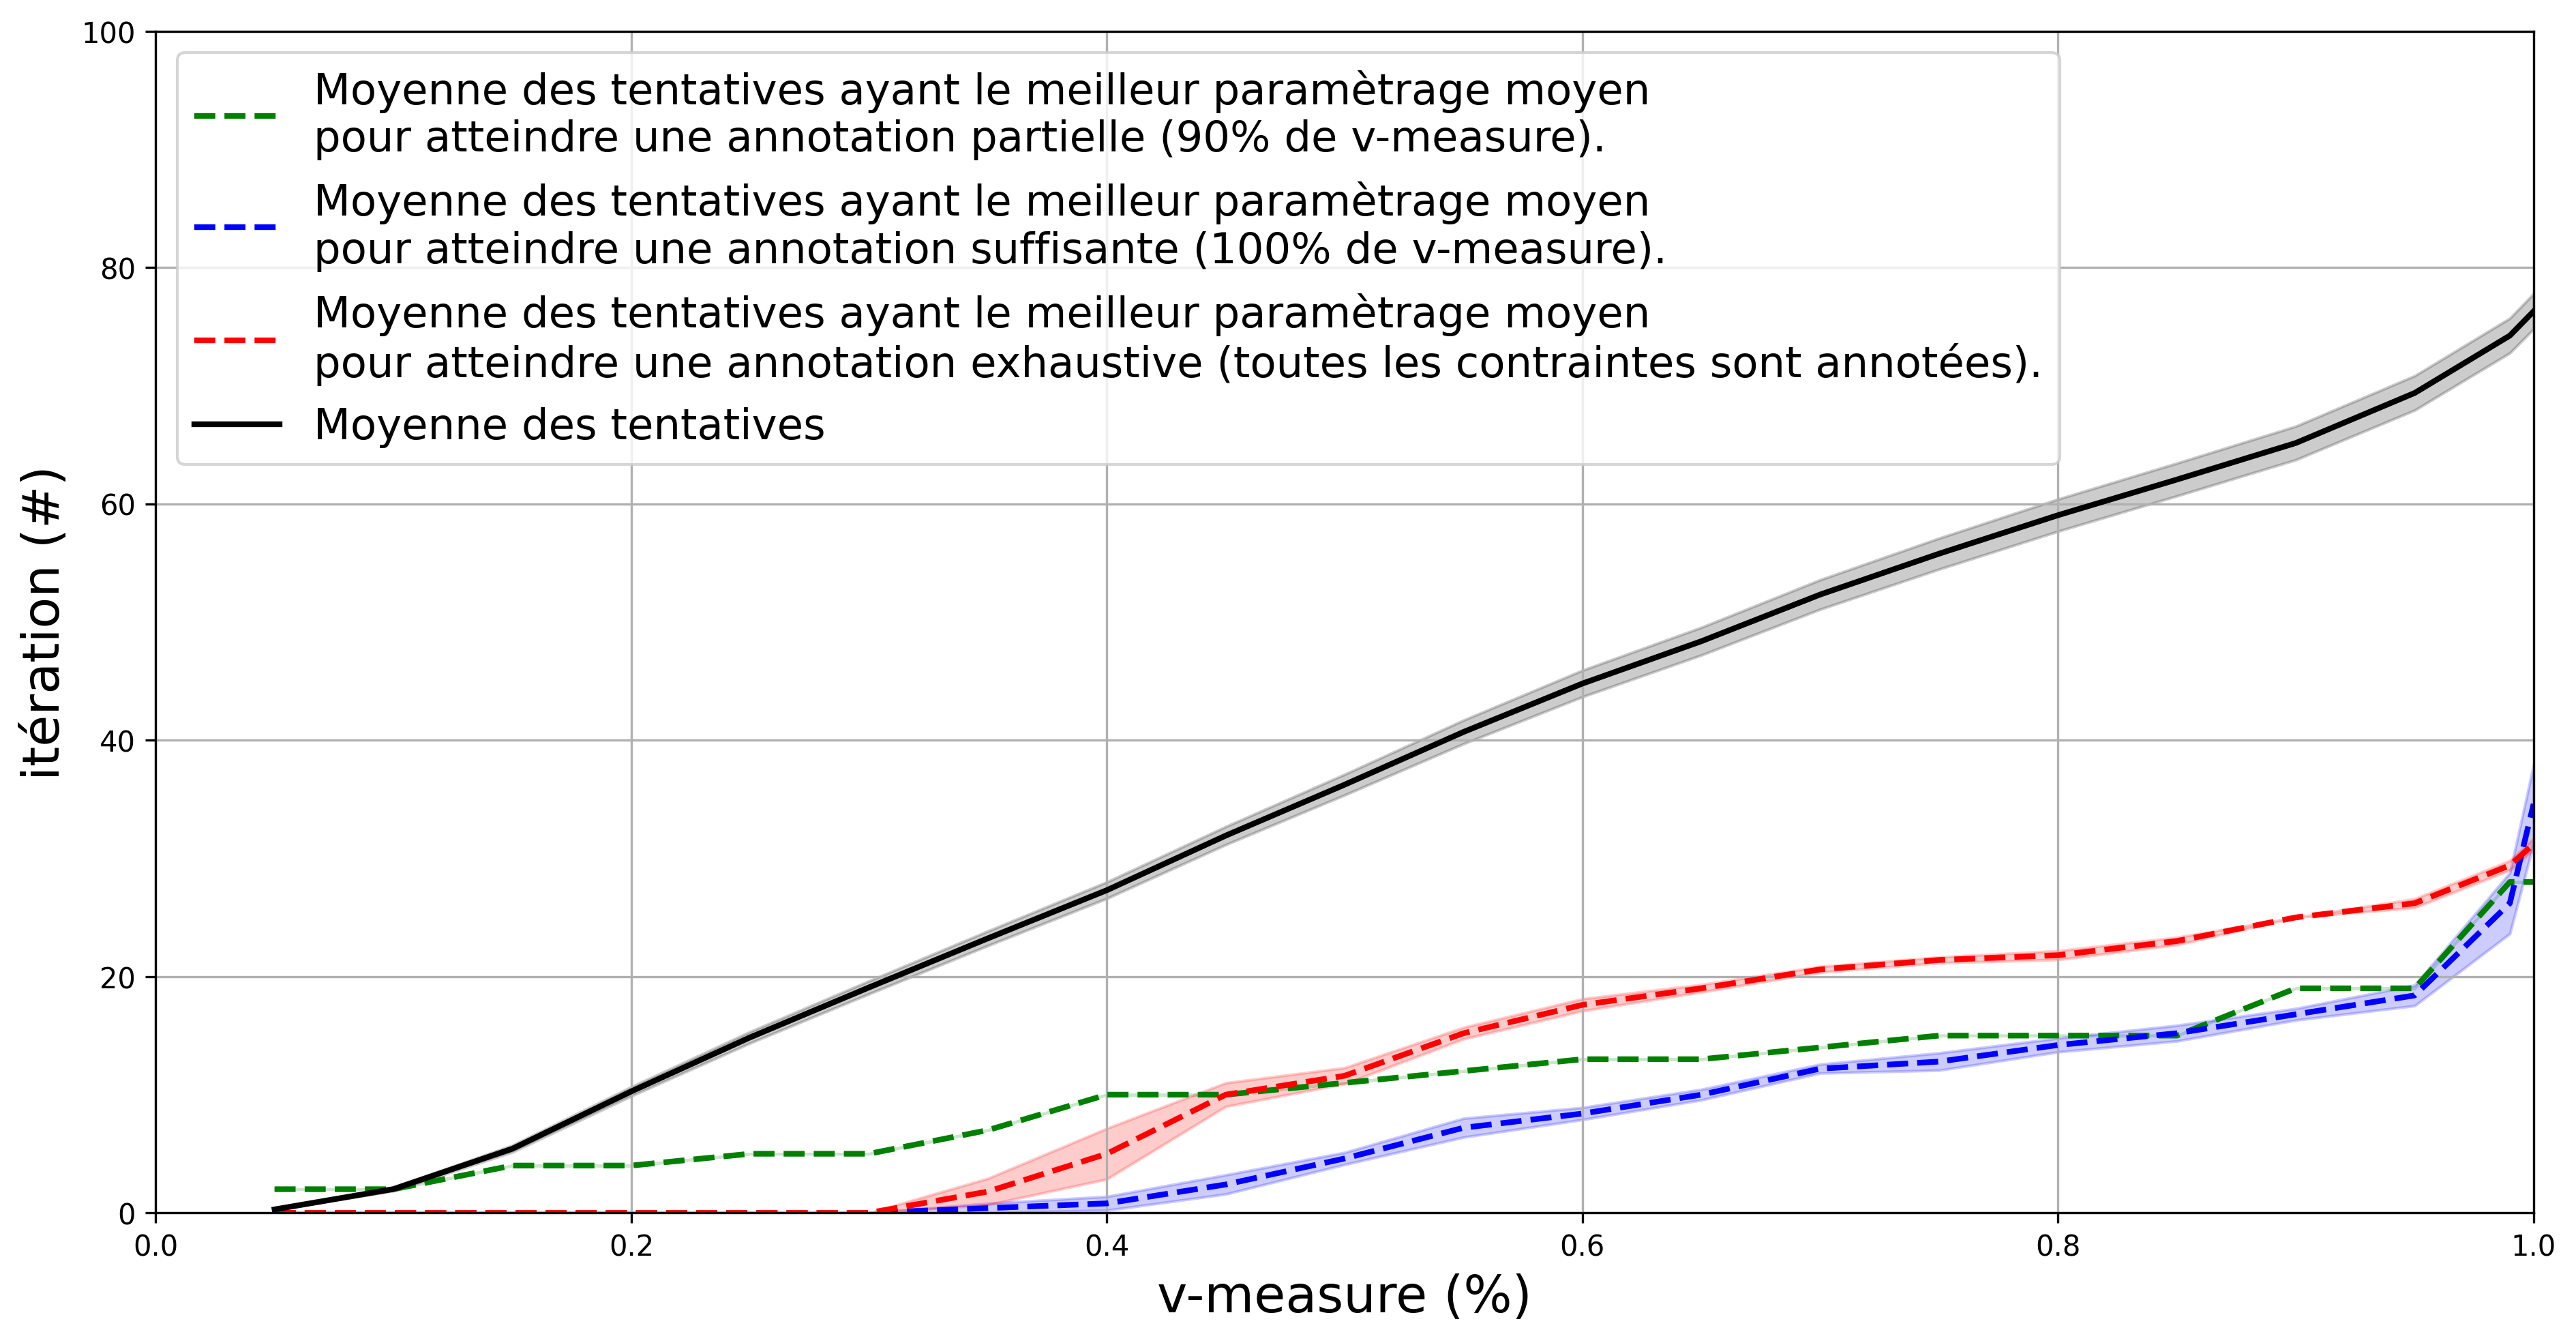
\includegraphics[width=0.95\textwidth]{figures/etude-efficience-evolution-moyenne-5best-par-vmeasure}
				\caption{Évolution des moyennes du nombre d'itérations nécessaire de la méthode de \textit{clustering} interactif pour obtenu un seuil défini de \texttt{v-measure} entre un résultat obtenu et la vérité terrain, moyennes réalisées sur les différentes seuils d'annotations étudiés : l'annotation partielle (\textit{atteindre une \texttt{v-measure} de $90$\%}), l'annotation suffisante (\textit{atteindre une \texttt{v-measure} de $100$\%}) et l'annotation exhaustive (\textit{annoter toutes les contraintes possibles}).}
				\label{figure:4.2.1-ETUDE-OPTIMISATION-EVOLUTION-MEILLEUR-PARAMETRAGE}
			\end{figure}

		%%% Discussion.
		\subsubsection{Discussion}

			% Rappel de l'objectif : être efficient.
			L'objectif de l'étude est de trouver une implémentation "efficiente" du \textit{clustering} interactif permettant d'obtenir une base d'apprentissage correctement annotée en un minimum d'annotation.
			Pour trouver si une telle implémentation existe et quels en sont les paramètres optimaux, nous avons analysé l'impact de différentes paramétrages sur les tâches principales de la méthode (\textbf{prétraitement}, \textbf{vectorisation}, \textbf{clustering sous contraintes}, \textbf{échantillonnage}) en nous basant sur des simulations d'annotation d'un jeu de données.
			
			% Première remarque : Choix d'un seuil à 90\% de v-measure.
			Dans l'optique d'être efficient, nous excluons le désir d'annoter \textbf{exhaustivement} le jeu de données car la charge de travail estimée est trop importante.
			(cf. discussion de la section~\ref{section:4.1-HYPOTHESE-EFFICACITE} (hypothèse d'efficacité))
			Nous préférons donc nous concentrer sur deux seuils d'annotation plus réalistes : celui d'une \textbf{annotation partielle} (atteindre $90$\% de \texttt{v-measure} avec la vérité terrain) et celui d'une \textbf{annotation suffisante} (atteindre $100$\% de \texttt{v-measure} avec la vérité terrain en un minimum de contraintes). 
			
			% Meilleur paramétrage.
			L'étude réalisée met en avant l'impact significatif des quatre tâches principales (\textbf{prétraitement}\todo{remarque sur la valeur de eta2}, \textbf{vectorisation}\todo{remarque sur la valeur de eta2}, \textbf{clustering sous contraintes}, \textbf{échantillonnage}) sur la vitesse de convergence de la méthode pour atteindre les seuils définis de $90$\% et $100$\% de \texttt{v-measure}. Il existe donc bien un paramétrage permettant d'optimiser l'implémentation proposée et de réduire le nombre de contraintes nécessaires à annoter :
			\begin{enumerate}
				\item pour une \textbf{annotation partielle} ($90$\% de \texttt{v-measure}), le meilleur paramétrage moyen est constitué du prétraitement simple (\texttt{prep.simple}), de la vectorisation TF-IDF (\texttt{vect.tfidf}), du \textit{clustering} hiérarchique à lien moyen (\texttt{clust.hier.avg}) et de l'échantillonnage des données les plus proches dans des clusters différents (\texttt{sampl.closest.diff}). Avec ce paramétrage, il faut en moyenne $950$ annotations de contraintes pour obtenir une \texttt{v-measure} de $90$\% ;
				\item pour une \textbf{annotation suffisante} ($100$\% de \texttt{v-measure}), le meilleur paramétrage moyen est constitué du prétraitement avec lemmatisation (\texttt{prep.lemma}), de la vectorisation TF-IDF (\texttt{vect.tfidf}), du \textit{clustering} KMeans avec modèle COP (\texttt{clust.kmeans.cop}) et de l'échantillonnage des données les plus proches dans des clusters différents (\texttt{sampl.closest.diff}). Avec ce paramétrage, il faut en moyenne $1~750$ annotations de contraintes pour obtenir une \texttt{v-measure} de $100$\% ;
				\item le cas d'une \textbf{annotation exhaustive} (annoter toutes les contraintes possibles sur les données) n'est pas explicité ici mais peut se déduire des résultats décrits plus haut.
			\end{enumerate}

			%%% Avantages.
			Ainsi, cette étude permet de répondre à la limite du nombre de contraintes requis (discutée dans l'hypothèse d'efficacité, section~\ref{section:4.1-HYPOTHESE-EFFICACITE}).
			%%% Avantage 1: Optimisation du nombre de contraintes.
			En effet, l'optimisation des paramètres de l'implémentation du \textit{clustering} interactif permet de réduire considérablement le nombre de contraintes nécessaires pour obtenir une base d'apprentissage exploitable.
			En nous basant sur le tableau~\ref{table:4.1.1-ETUDE-CONVERGENCE-EVOLUTION} de l'étude de convergence, et dans le cadre de l'annotation d'un jeu de $500$ données, nous sommes passé d'un paramétrage moyen nécessitant $3~750$ (respectivement $10~000$) contraintes à un paramétrage optimisé ne nécessitant que $950$ (respectivement $1~750$) contraintes pour atteindre un seuil de $90$\% (respectivement $100$\%) \texttt{v-measure}.
			L'ordre de grandeur de la charge de travail demandée aux annotateurs est donc située entre $2$ et $4$ fois la taille du jeu de données.
			
			% Avantage 2: La méthode devient réaliste !
			Cette estimation est plus raisonnable que celle réalisée en section~\ref{section:4.1-HYPOTHESE-EFFICACITE}.
			De plus, en considérant que les annotations sont binaires et demandent a priori une charge mental plus faible que les annotations par attribution de label ("\textit{les données sont-elles similaires ?}" vs "\textit{quel est l'étiquette de cette donnée ?}", cf. CITATION)\todo{CITATION: Development of NASA-TLX (Task Load Index): Results of Empirical and Theoretical Research}, nous pouvons espérer que la charge totale nécessaire à l'annotation avec une méthodologie basée sur le \textit{clustering} interactif est comparable à celles des méthodes traditionnelles.
			
			%%% Limites.
			Afin de compléter cette analyse d'efficience, quelques pistes sont encore à explorer.
			
			% Limite 1 : Coût temporel.
			D'une part, une étude de coût est à réaliser pour trancher le choix de paramètre optimaux réalistes.
			En effet, il est intéressant d'étudier le coût machine (temps CPU utilisé) et le coût humain (temps d'annotation) afin d'affiner les choix techniques et de compléter les arguments sur l'utilisation en situation réelle d'une méthodologie d'annotation basée sur le \textit{clustering} interactif.
			Cette étude sera l'occasion de rentrer en détail dans la comparaison de la charge demander à l'annotateur, tant sur la durée que sur la complexité de la tâche d'annotation.
			Cet aspect sera traité dans la section~\ref{section:4.3-HYPOTHESE-COUTS} (hypothèse des coûts).
			
			% Limite 2 : Valeur métier de ce 90\% (pas de vérité terrain en pratique).
			D'autre part, l'étude réalisée se base sur des seuils de performance par rapport à une vérité terrain.
			Or en situation réelle, cette comparaison avec la vérité terrain n'est pas possible car elle est précisément en cours de conception (la base d'apprentissage finale devant être la vérité terrain).
			De plus, un tel score n'est pas le plus explicite pour pour un expert métier pour qui un score de \texttt{v-measure} n'est pas révélateur de la pertinence métier de la segmentation proposée des données.
			Dans un registre similaire, il est possible que l'évolution du partitionnement des données passe par plusieurs états stables et pertinents, mais que l'annotateur soit obligé d'affiner sa vision en annotant certaines contraintes ambiguës.
			Cela peut être la cas avec des \textit{clusters} traitant en fin de compte de sujets très similaires (\textit{ajouter des \texttt{MUST-LINK} pour les fusionner}) ou avec un \textit{cluster} qui regroupe finalement plusieurs thématiques (\textit{ajouter des \texttt{CANNOT-LINK} pour le segmenter})
			Il manque donc une stratégie d'évaluation de pertinence de la base d'apprentissage en cours de construction afin d'estimer la stabilité d'un partitionnement et de la suffisance des annotations réalisées pour faire refléter la vision de l'annotateur dans le résultat obtenu.
			Cet aspect sera traité dans la section~\ref{section:4.4-HYPOTHESE-PERTINENCE} (hypothèse de pertinence).
			
			% Limite 3 : Expert métier parfait ==> simuler les erreurs.
			Pour finir, comme pour l'étude de convergence réalisé en section~\ref{section:4.1-HYPOTHESE-EFFICACITE}, nous avons supposé dans cette étude que l'annotateur est un expert métier connaissant parfaitement le domaine traité.
			Cette hypothèse forte n'est a priori pas valable en situation réelle : En effet, des erreurs d'annotations peuvent intervenir (ambiguïtés sur les données, méconnaissance du domaine, erreurs d'inattention, différence d'opinions entre annotateurs, ...), ce qui peut entraîner des divergences ou des incohérences dans la construction de la base d'apprentissage.
			Il semble donc nécessaire d'étudier les impacts de ces incohérences, ainsi que de proposer une méthode pour les prévenir ou les corriger.
			Cet aspect sera traité à la fin de ce chapitre dans la section~\ref{section:4.6-HYPOTHESE-ROBUSTESSE} (hypothèse de robustesse).
	
	
	%%%%%--------------------------------------------------------------------
	%%%%% Section 4.3: Hypothèse sur les coûts.
	%%%%%--------------------------------------------------------------------
	\newpage
	\section{Évaluation de l'hypothèse sur les coûts}
\label{section:4.3-HYPOTHESE-COUTS}

	%%%
	%%% Introduction / Transition.
	%%%
	Dans les deux sections précédentes, nous avons estimé le paramétrage du \textit{clustering} interactif le plus efficient pour atteindre $90$\% de \texttt{v-measure} avec la vérité terrain, correspondant à ce que nous appelons une annotation partielle.
	Toutefois, pour compléter l'étude de faisabilité technique de notre méthode, nous devons nous intéresser aux coûts (matériel et humain) à investir pour atteindre notre objectif.
	Nous aimerions donc vérifier l'hypothèse suivante :
	
	%%%
	%%% Formulation des hypothèses.
	%%%
	\begin{tcolorbox}[
		title=\faVial~\textbf{Hypothèse sur les coûts}~\faVial,
		colback=colorTcolorboxHypothesis!15,
		colframe=colorTcolorboxHypothesis!75,
		width=\linewidth
	]
		% Hypothèse.
		\textguillemets{\textbf{
			Il est possible d'estimer les coûts nécessaires d'une méthodologie d'annotation basée sur le \textit{clustering} interactif pour obtenir une base d'apprentissage exploitable.
			Nous étudions en particulier les coûts relatifs au temps d'annotation, au temps de calculs des algorithmes, ainsi que la durée totale de la méthode en fonction de la taille du jeu de données.
		}} \\
		
		% Figure.
		La \textsc{Figure~\ref{figure:4.3-HYPOTHESE-COUTS}} illustre cette hypothèse et l'espoir de pouvoir caractériser la qualité de la base d'apprentissage en cours de construction en fonction d'un coût temporel au lieu d'un nombre abstrait d'itérations de la méthode. 
		%
		\begin{figure}[H]  % keep [H] to be in the tcolorbox.
			\centering
			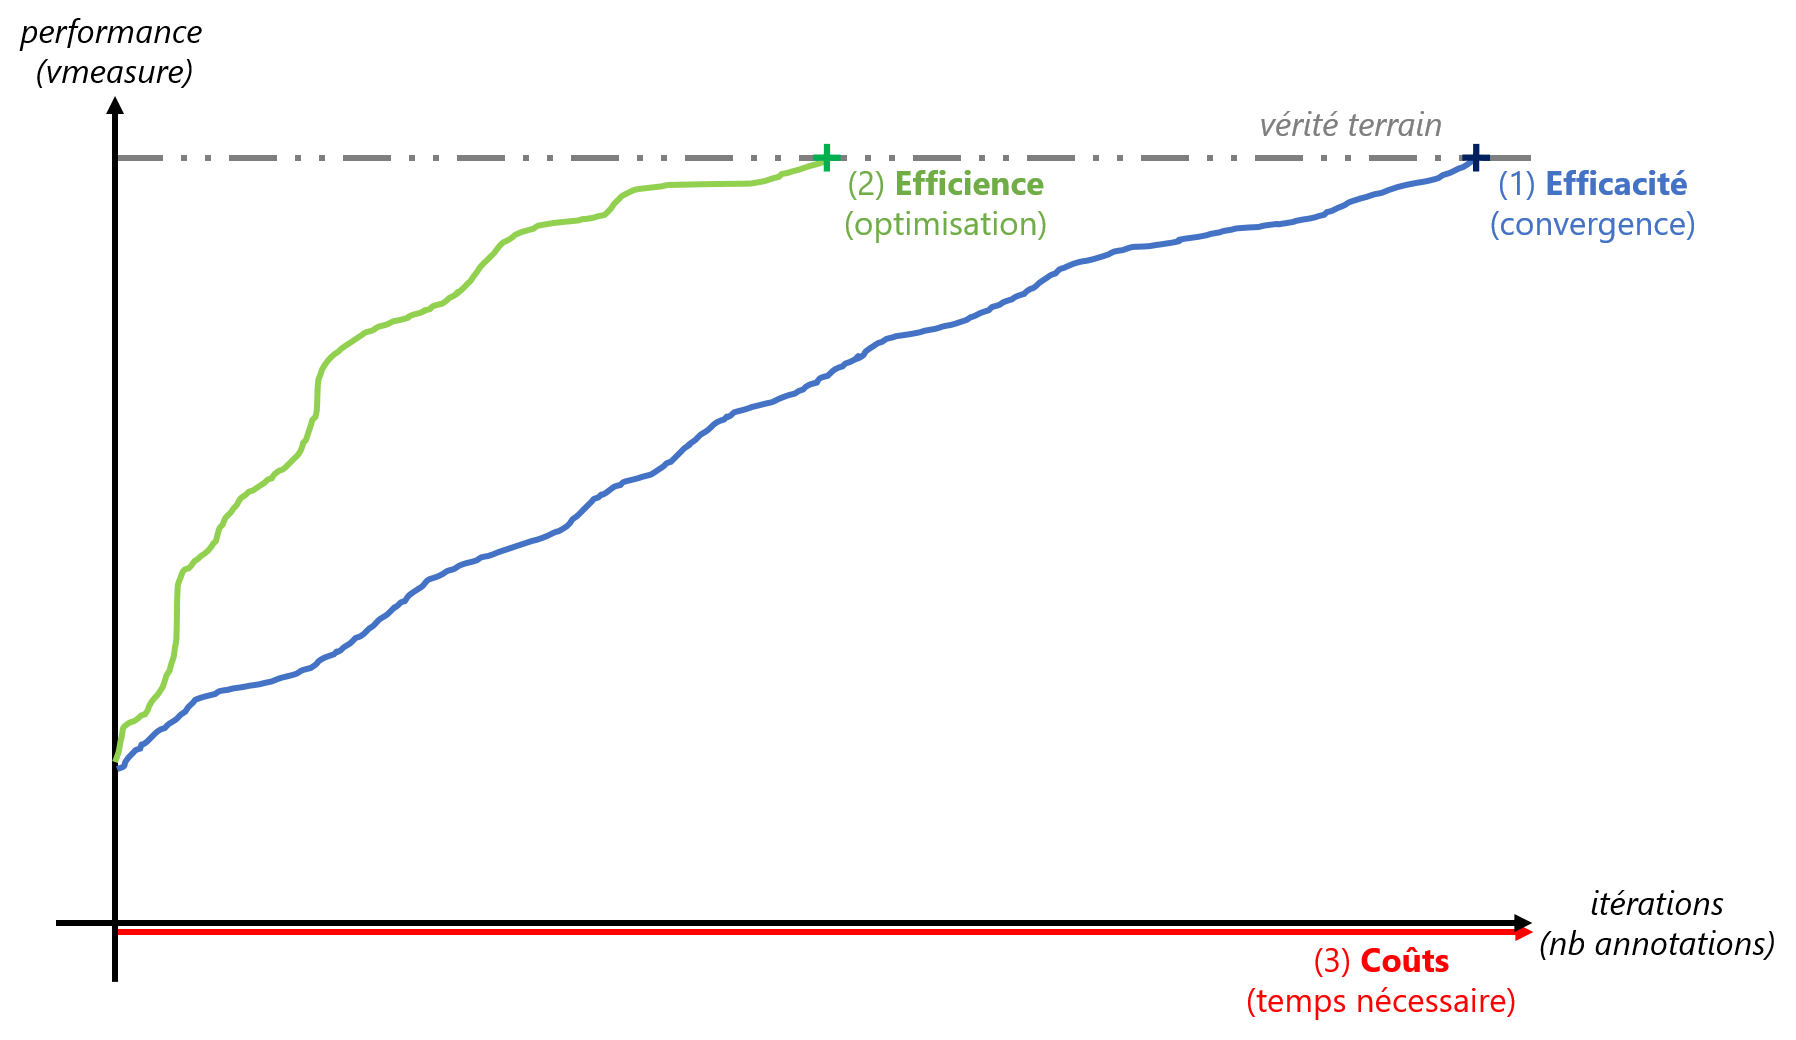
\includegraphics[width=0.95\textwidth]{figures/hypotheses-03-couts}
			\caption{
				Illustration des études réalisées sur le \textit{clustering} interactif (\textit{étape 3/6}) en schématisant l'évolution de la performance (\textit{accord avec la vérité terrain calculé en v-measure}) d'une base d'apprentissage en cours de construction en fonction du coût temporel de la méthode (\textit{temps nécessaire à l'expert métier et à la machine}).
			}
			\label{figure:4.3-HYPOTHESE-COUTS}
		\end{figure}
	\end{tcolorbox}

	% Résumé des études.
	Afin de vérifier cette hypothèse, nous organisons plusieurs expériences pour simuler et déterminer ces durées :
	\begin{itemize}
		\item une étude du \textbf{temps d'annotation} par un expert métier, mesuré lors d'une expérience d'annotation de contraintes faisant intervenir plusieurs opérateurs (cf. \textsc{Section~\ref{section:4.3.1-ETUDE-COUTS-TEMPS-ANNOTATION}}) ;
		\item une étude du \textbf{temps de calcul} des algorithmes, modélisé en exécutant les différentes implémentations du \textit{clustering} interactif avec diverses valeurs d'arguments (cf. \textsc{Section~\ref{section:4.3.2-ETUDE-COUTS-TEMPS-CALCUL}}) ;
		\item et une étude du \textbf{nombre de contraintes} nécessaires en fonction du nombre de données à traiter, estimé en simulant la création d'une base d'annotation avec notre méthodologie sur des jeux de données de différentes tailles (cf. \textsc{Section~\ref{section:4.3.3-ETUDE-COUT-NOMBRE-CONTRAINTES}}).
	\end{itemize}
	Nous exposons nos conclusions sur l'estimation du \textbf{temps total} à investir et réalisons une comparaison avec une organisation plus traditionnelle d'un projet d'annotation en \textsc{Section~\ref{section:4.3.4-ETUDE-COUTS-TOTAL}}.
	
	
	%%%
	%%% Subsection 4.3.1: Étude du temps d'annotation nécessaire pour traiter un lot de contraintes en chronométrant des opérateurs en situation réelle
	%%%
	\subsection{Étude du temps d'annotation nécessaire pour traiter un lot de contraintes en chronométrant des opérateurs en situation réelle}
	\label{section:4.3.1-ETUDE-COUTS-TEMPS-ANNOTATION}
		
		% Objectif de l'expérience.
		Nous voulons estimer le temps nécessaire à un opérateur pour annoter un lot de contraintes.
		Pour cela, nous allons chronométrer plusieurs experts métiers en train d'annoter un même échantillon et modéliser le nombre de contraintes par minute, ainsi que son évolution au cours de plusieurs sessions d'annotation.
		De plus, nous aimerions aussi confirmer que l'ajout de contraintes dans notre contexte s'apparente à une tâche "intuitive", c'est-à-dire que l'annotation se fait dans la réaction et non dans la réflexion (voir \cite{kahneman:2011:thinking-fast-slow} qui distingue un \textit{système 1} intuitif, rapide, de l'ordre de l'émotion, et un \textit{système 2} plus lent, logique et réfléchi).
		Pour ce faire, nous estimons grossièrement le temps nécessaire à l'annotation réactive d'une contrainte, nous le comparons au temps moyen estimé lors de notre expérience, et nous nous demandons si la différence observée peut cacher un mécanisme cognitif plus complexe.
	
		%%% Protocole expérimental.
		\subsubsection{Protocole expérimental}
			
			% Axiome.
			\begin{leftBarWarning}
				Dans cette étude, nous supposons que les annotateurs de l'expérience connaissent parfaitement le domaine traité dans le jeu de données, et qu'ils sont capables de caractériser sans ambiguïté la similitude entre deux données issues de cet ensemble.
				Afin de pourvoir faire cette hypothèse forte, et ainsi limiter les bruits dans l'analyse des résultats, le jeu de données devra traiter d'un sujet de culture générale (ne nécessitant donc pas de connaissance particulière) et des réviseurs supprimeront en amont et d'un commun accord les données trop spécifiques ou trop ambiguës.
			\end{leftBarWarning}
			
			% Pseudo-code.
			Pour résumer le protocole expérimental que nous décrivons ci-dessous, vous pouvez vous référer au pseudo-code décrit dans \textsc{Algorithme~\ref{algorithm:4.3.1-ETUDE-COUTS-TEMPS-ANNOTATION-PROTOCOLE}}.

			\begin{algorithm}
				\KwData{jeu de données annotées (vérité terrain)}
				\KwIn{plusieurs réviseurs, plusieurs annotateurs}
				%
				\textbf{initialisation}: définir et revoir le jeu de données entre réviseurs \;
				\textbf{échantillonnage}: sélectionner une base de contraintes avec \texttt{samp.rand.full} \;
				\textbf{temps théorique}: estimation du temps nécessaire à l'annotation d'une contrainte \;
				\ForEach{annotateur}{
					 \While{la base de contraintes n'a pas été entièrement annotée}{
						\textbf{chronomètre}: \textbf{START} \;
						\textbf{annotation}: annoter une partie des contraintes \;
						\textbf{revue}: revue des contraintes en conflits d'annotation \;
						\textbf{chronomètre}: \textbf{STOP} \;
						\textbf{mesure}: estimer la différence de chronomètre pour cette session \;
					}
				}
				\textbf{analyse}: modéliser le temps d'annotation d'un lot de contraintes \;
				%
				\KwResult{modélisation du temps d'annotation d'un lot de contraintes}
				%
				\caption{\textit{
					Description en pseudo-code du protocole expérimental de l'étude du temps d'annotation d'un lot de contraintes par plusieurs experts métiers en situation réelle.
				}}
				\label{algorithm:4.3.1-ETUDE-COUTS-TEMPS-ANNOTATION-PROTOCOLE}
			\end{algorithm}
			
			% Détails de l'expérience : préparation du jeu de données.
			Nous allons procéder en plusieurs étapes.
			D'abord, il faut choisir un jeu de données approprié : pour valider notre hypothèse forte sur les compétences de nos annotateurs, nous cherchons un jeu de données traitant d'un sujet de culture général.
			Pour cette expérience, nous avons donc choisi \texttt{MLSUM} : une collecte d'articles de journaux, classés par catégorie de publication et décrits par leur titre et leur résumé.
			Nous nous intéressons ici à la tâche de classification d'un titre d'article en fonction de sa catégorie de publication.
			Comme certains titres peuvent porter à confusion (un titre d'article n'étant pas toujours explicite sur son contenu), deux réviseurs sont chargés de choisir les données les plus explicites sur un échantillon d'un millier de données représentatives des catégories les plus communes.
			L'échantillon résultant, noté \texttt{MLSUM FR Train Subset (v1.0.0-schild)}, est composé de $744$ titres d'articles rédigés en français et répartis en $14$ classes (\textit{économie}, \textit{sport}, ...).
			Pour plus de détails, consultez l'annexe~\ref{annex:A.2-DATASET-MLSUM-SUBSET-SCHILD}.
			
			% Détails de l'expérience : sélection des contraintes à annoter.
			À partir de ces données, nous sélectionnons un lot de $1~000$ contraintes à annoter.
			Comme nous nous intéressons exclusivement au temps d'annotation pour cette expérience (et que nous ne regardons pas le nombre d'itérations de la méthode), nous utilisons l'échantillonnage purement aléatoire (\texttt{samp.rand.full}).
			L'analyse de l'accord inter-annotateurs sera réalisé en \textsc{Section~\ref{section:4.6.3-ETUDE-ROBUSTESSE-SCORE-INTER-ANNOTATEURS}}.
			
			% Détails de l'expérience : estimation du temps théorique nécessaire à l'annotation d'une contrainte.
			Sur la base de cette échantillon, nous pouvons approximer le temps théorique nécessaire à l'annotation d'une contrainte à $6.8$ secondes.
			En effet, il faut d'abord considérer la taille moyenne des titres d'article à lire et en déduire le temps dédié à la lecture des deux textes de la contraintes.
			En utilisant l'approximation d'une lecture silencieuse par un adulte à $238$ mots par minute (\cite{brysbaert:2019:how-many-words}) et en mesurant la taille moyenne des titre d'article à $10.1$ mots, on en déduit que le temps de lecture d'un texte est environ de $2.55$ secondes.
			Ensuite, il convient d'intégrer la durée de traitement cognitif requis pour estimer si les deux phrases sont similaires ou discordantes.
			À cet effet, nous retenons $1$ seconde\footnote{
				Nous pourrions faire le parallèle avec la composante \texttt{P600} communément admise en neuroscience pour caractériser la réaction provoquée par la dissonance grammaticale ou syntaxique d'une phrase.
				Nous arrondissons à $1$ seconde pour garder une marge d'erreur.
			} (\cite{purves-brannon:2013:principles-cognitive-neuroscience})
			en admettant que cette tâche est rapide.
			Enfin, nous ajoutons $1$ seconde supplémentaire pour représenter la réaction motrice (clic de bouton) et le délais applicatif (rechargement de la page).
			Au total, nous obtenons ainsi un temps d'annotation moyen de $7$ secondes.
			Bien entendu, cette durée reste approximative, mais elle nous permet de discuter de l'ordre de grandeur à manipuler durant l'annotation.
			
			% Détails de l'expérience : annotations et consignes.
			Ensuite, un groupe de $14$ annotateurs vont annoter la sélection de $1~000$ contraintes en plusieurs sessions.
			Les directives données aux opérateurs sont les suivantes:
			\begin{itemize}
				\item \textbf{Contexte de l'opérateur} :
				\textguillemets{\textit{Vous êtes des \textbf{experts de la presse et de l'actualité} ; Vous voulez classer des articles dans des catégories en fonction de leur titre ; Vous ne savez pas précisément quelles catégories vous allez utiliser pour classer vos articles ; Mais vous savez \textbf{caractériser la similitude} de deux articles}} ;
				\item \textbf{Contexte sur le jeu de données} :
				\textguillemets{\textit{Le thème sont les catégories d'articles de presse ; La vérité terrain contient entre $10$ et $20$ catégories parmi les plus communes de la presse ; La vérité terrain contient entre $30$ et $100$ articles par catégorie ; Vous \textbf{pouvez regarder le jeu de données non annoté} autant que vous le voulez (disponible dans l'onglet \texttt{TEXTS} de l'application)}} ;
				\item \textbf{Objectif de l'expérience} :
				\textguillemets{\textit{Je veux savoir le temps nécessaire pour annoter un certain nombre de contraintes ; Autrement dit : \textbf{Pour annoter 1000 contraintes, combien de temps me faut-il ?}}} ;
				\item \textbf{Consignes d'annotations} :
				\textguillemets{\textit{Faites des séries de \textbf{15 minutes minimum} pour avoir de la régularité ; Si possible, \textbf{isolez-vous} pour ne pas être dérangé et ne pas fausser les résultats ; Pour chaque série, \textbf{notez le temps et le nombre de contraintes annotés} ; Si vous ne savez pas quoi annoter (trop ambigu, vocabulaire inconnu, ...), \textbf{passez au suivant sans annoter} (vous êtes sensés être des experts de la presse !)}}.
			\end{itemize}
			%
			Pour réaliser l'annotation, les opérateurs auront accès à l'application web développée au cours de ce doctorat.
			Des captures d'écran sont disponibles en \textsc{Figure~\ref{figure:4.3.1-ETUDE-COUTS-TEMPS-ANNOTATION-APPLICATION-ANNOTATION}} et \textsc{Figure~\ref{figure:4.3.1-ETUDE-COUTS-TEMPS-ANNOTATION-APPLICATION-LISTE-CONTRAINTES}}.
			Une description plus détaillée de l'application et de ses fonctionnalités est disponible en \textsc{Section~\ref{section:3.3-DESCRIPTION-IMPLEMENTATION}}\todo{description à faire}.
			%
			\begin{figure}[!htb]
				\centering
				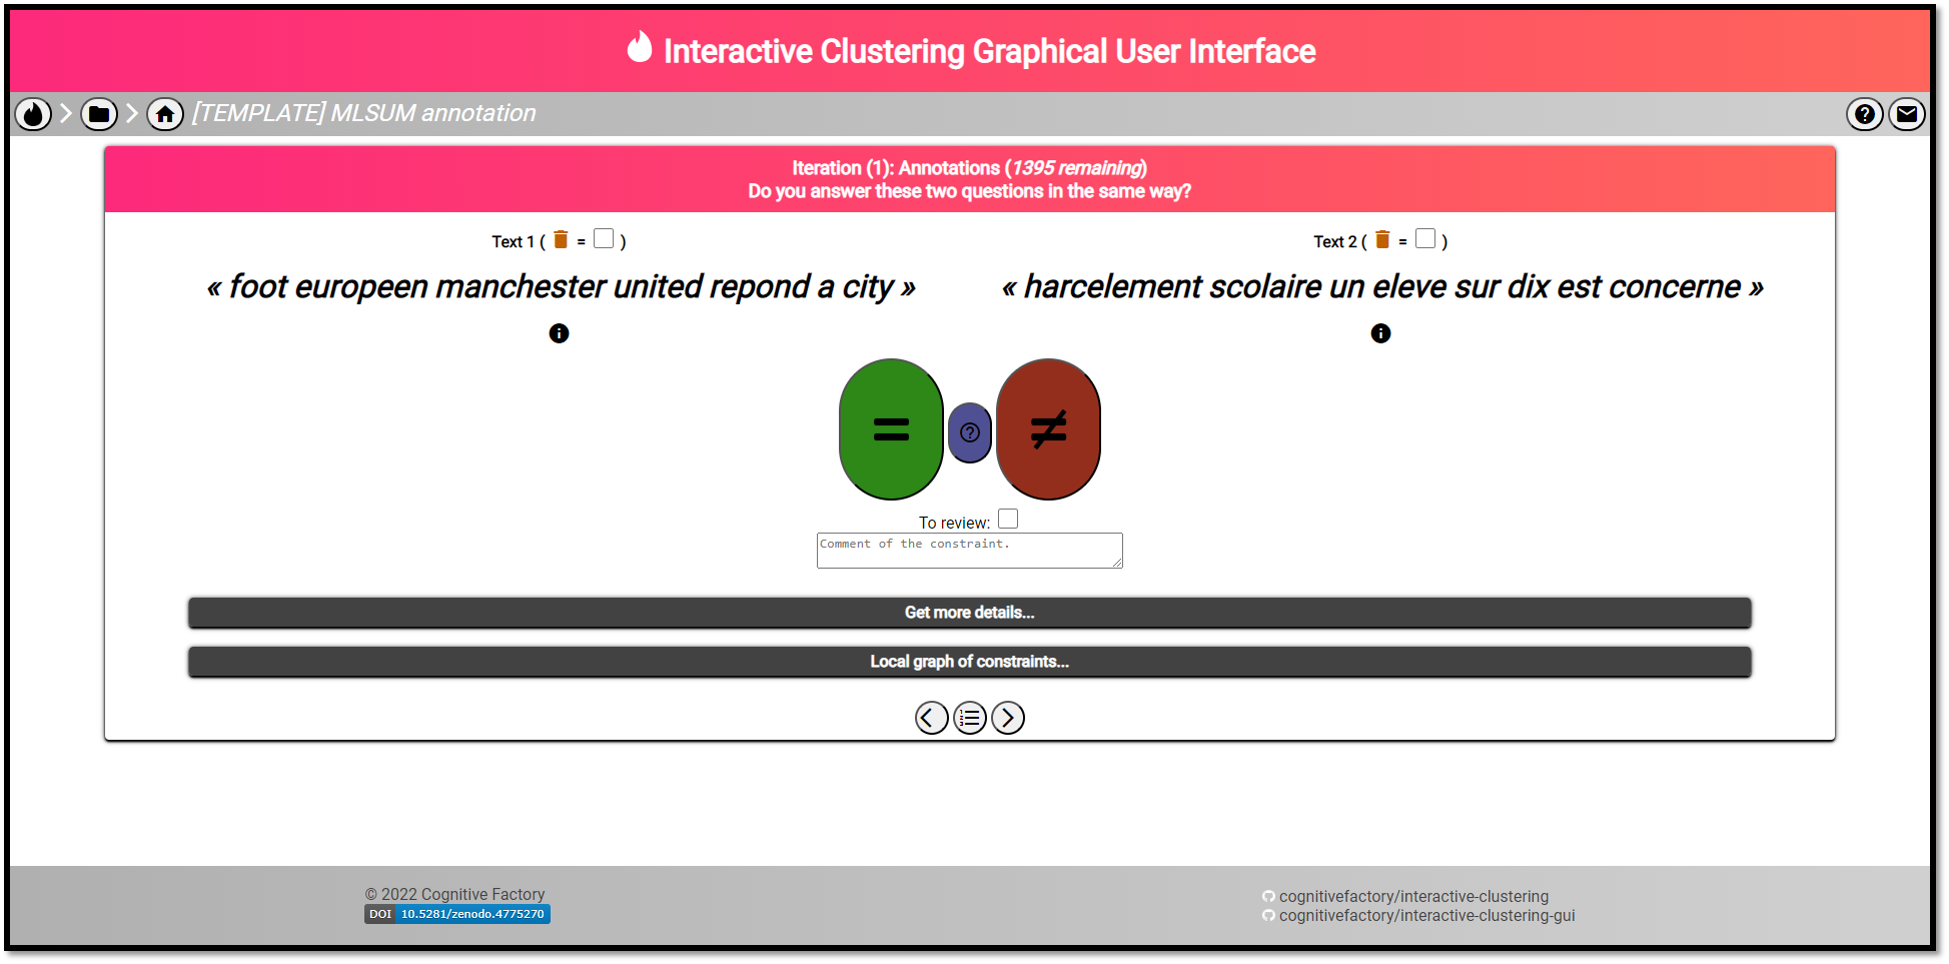
\includegraphics[width=0.95\textwidth]{figures/etude-temps-annotation-0application-annotation}
				\caption{
					Capture d'écran de l'application web permettant utilisant notre méthodologie de \textit{clustering} interactif pour annoter des contraintes (page d'annotation). Les deux textes à annoter sont disposés à gauche et droite de l'écran. Chacun dispose d'un cache à cocher si le texte n'est pas pertinent à analyser (\textit{ambigu, hors périmètre, incompréhensible, ...}).\\
					Les boutons à disposition permettent respectivement d'annoter un \texttt{MUST-LINK} si les données sont similaires (\textit{bouton en vert}), un \texttt{CANNOT-LINK} si les données ne sont pas similaire (\textit{bouton en rouge}), d'ignorer la contrainte pour laisser la main à l'algorithme de \textit{clustering} (\textit{bouton en bleu}), et d'ajouter un commentaire pour revoir la contrainte plus tard (\textit{case à choser et champ de texte libre}). Deux éléments déroulant permettent d'avoir des informations supplémentaires (\textit{metadata de sélection et de \textit{clustering}, représentation graphique des liens entre contraintes annotées}). Les boutons de navigation (\textit{boutons flèches et liste}) sont disponibles en bas de page.
				}
				\label{figure:4.3.1-ETUDE-COUTS-TEMPS-ANNOTATION-APPLICATION-ANNOTATION}
			\end{figure}
			\begin{figure}[!htb]
				\centering
				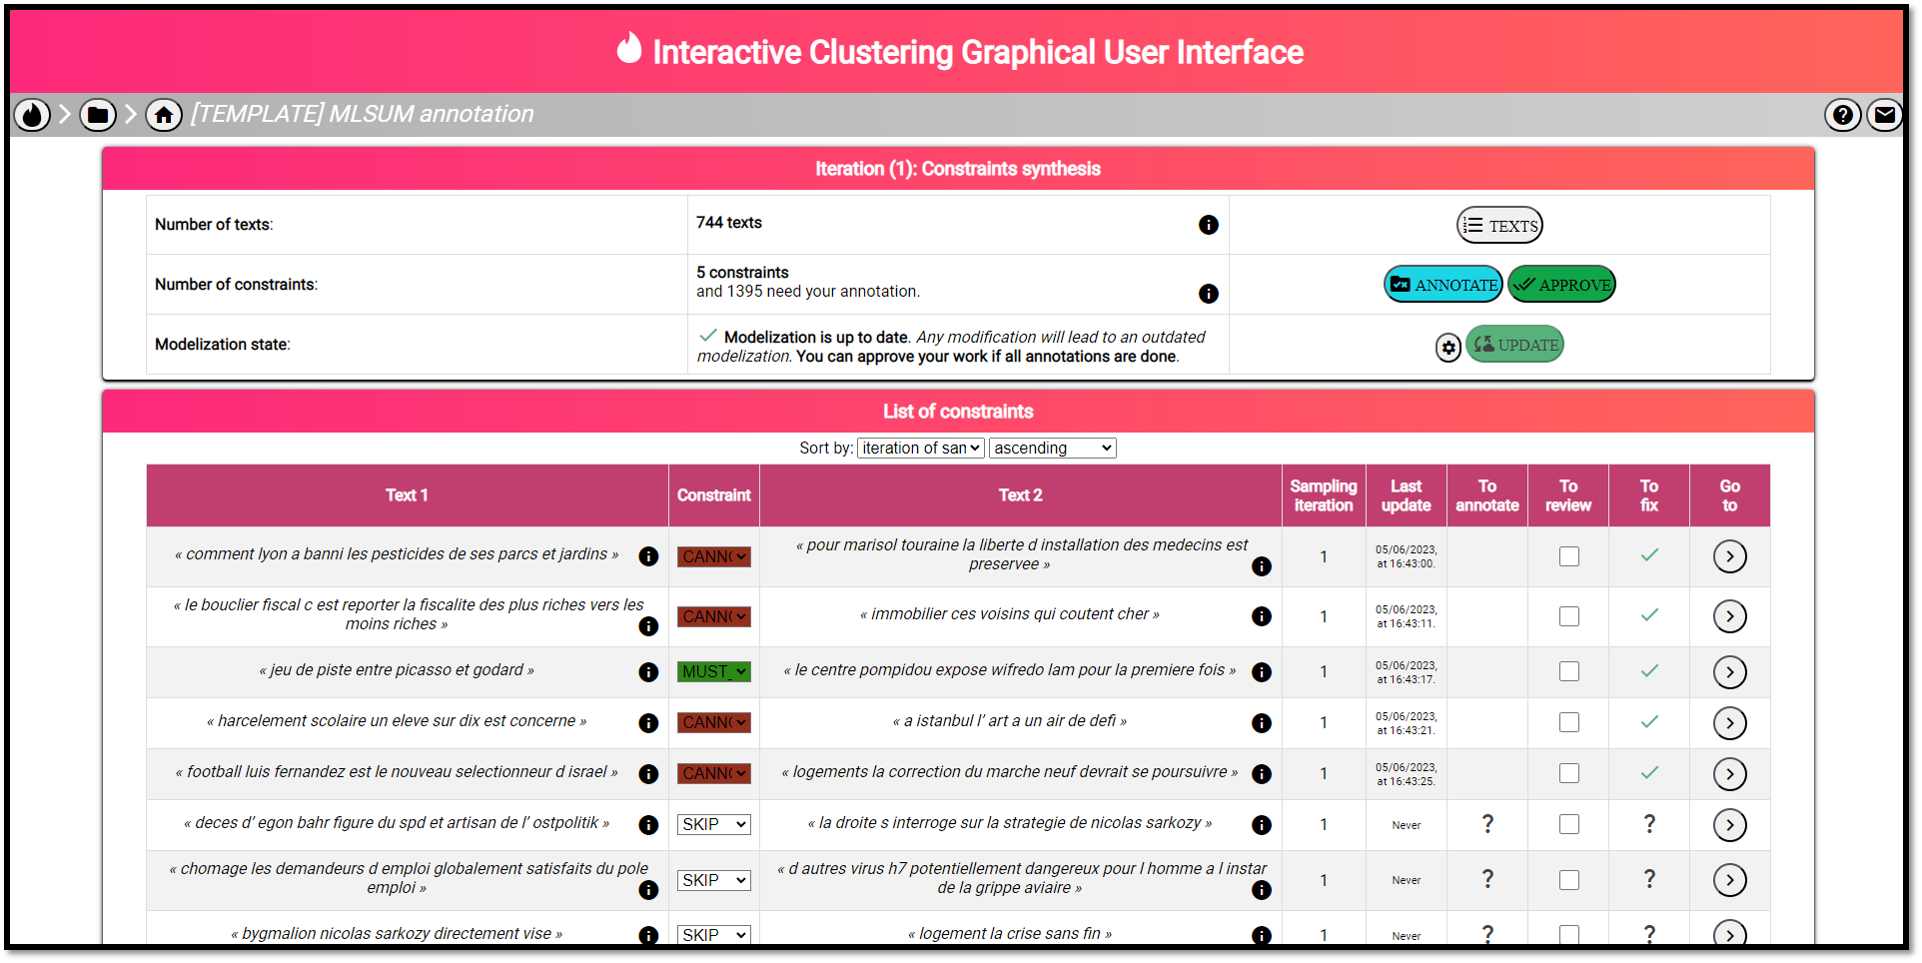
\includegraphics[width=0.95\textwidth]{figures/etude-temps-annotation-0application-liste-contraintes}
				\caption{
					Capture d'écran de l'application web permettant utilisant notre méthodologie de \textit{clustering} interactif pour annoter des contraintes (page d'inventaire des contraintes à annoter).\\
					La partie supérieure permet d'identifier le nombre de textes et de contraintes sur le projet, ainsi que les boutons destinés à calculer les transitivités entre les contraintes et à approuver le travail réalisé si aucune transitivité n'entre en conflit avec un contrainte annotée. La partie inférieure liste l'ensemble des contraintes du projet, avec les annotations réalisées, l'itération à laquelle la contraintes a été sélectionnée et annotée, si elle est à revoir ou si une incohérence la concernant est détectée.
				}
				\label{figure:4.3.1-ETUDE-COUTS-TEMPS-ANNOTATION-APPLICATION-LISTE-CONTRAINTES}
			\end{figure}
			
			
			% Détails de l'expérience : modélisation.
			Une fois les sessions d'annotations terminées, nous entraînons un modèle linéaire généralisé (\textit{GLM}) pour estimer le temps d'annotation moyen pour un lot de contraintes (dont la taille est notée $\texttt{batch\_size}$).
			Ce modèle sera caractérisé par le coefficient de détermination généralisé \texttt{R²} de \textit{Cox et Snel} (\cite{diamond-etal:1990:analysis-binary-data}), la log-vraisemblance \texttt{llf} (\cite{edwards:1992:likelihood}) et la log-vraisemblance \texttt{llf\_null} du modèle \textit{null}.
			Nous discutons aussi de l'évolution de la vitesse d'un opérateur au cours des différentes sessions d'annotation.

			% Référence scripts.
			\begin{leftBarInformation}
				L'outil d'annotation utilisé est accessible dans~\cite{schild-etal:2022:cognitivefactory-interactiveclusteringgui}.
				Les scripts de l'expérience, réalisés avec des \textit{notebooks} Python (\cite{van-rossum-drake:2009:python-reference-manual}), ainsi que le projet à importer dans l'outil d'annotation, sont disponibles dans un dossier dédié de~\cite{schild:2021:cognitivefactory-interactiveclusteringcomparativestudy}.
				Nous utilisons entre autres les librairies \texttt{datetime} et \texttt{statsmodels} (\cite{seabold-perktold:2010:statsmodels-econometric-statistical}).
			\end{leftBarInformation}

		%%% Résultats.
		\subsubsection{Résultats obtenus}
		
			% Taux de participation.
			Durant cette expérience, $14$ annotateurs ont participé à l'annotation de $1~000$ contraintes aléatoires sur un jeu de données.
			Par manque de disponibilités, $4$ annotateurs n'ont que partiellement réalisé leur tâche : nous avons toutefois intégré leurs participations car elles contenaient toutes au moins $150$ annotations.
			
			% Statistiques descriptives.
			D'après les observations, un annotateur réalisait en moyenne $170.7$ contraintes par session d'annotation (min: $43$, max: $547$, médiane: $138$, écart-type: $106.4$) ce qui lui demandait en moyenne $23.1$ minutes (min: $3.0$, max: $92.0$, écart-type: $14.4$).
			De plus, la vitesse d'annotation moyenne était de $7.7$ contraintes par minute (min: $3.5$, max: $14.3$, écart-type: $2.9$).
			
			% Modélisation du temps d'annotation.
			Le modèle linéaire généralisé entraîné sur les mesures de temps d'annotations (\texttt{R²}: $0.910$, \texttt{llf}: $-499.15$, \texttt{llf\_null}: $-539.95$) nous permet de déduire l'équation suivante :
			%
			\begin{equation}
				\label{equation:4.3.1-ETUDE-COUT-COUTS-TEMPS-ANNOTATION}
				\texttt{annotation\_time}~[s]~
				\propto~7.8 \cdot \texttt{batch\_size}
			\end{equation}
		
			% Affichage du temps d'annotation.
			La \textsc{Figure~\ref{figure:4.3.1-ETUDE-COUTS-TEMPS-ANNOTATION-SIMULATION}} représente cette modélisation du temps d'annotation en comparaison avec les mesures réalisées lors de l'expérience.
			Pour rappel, le temps théorique estimé précédemment est de $7$ secondes par contrainte.
			%
			\begin{figure}[!htb]
				\centering
				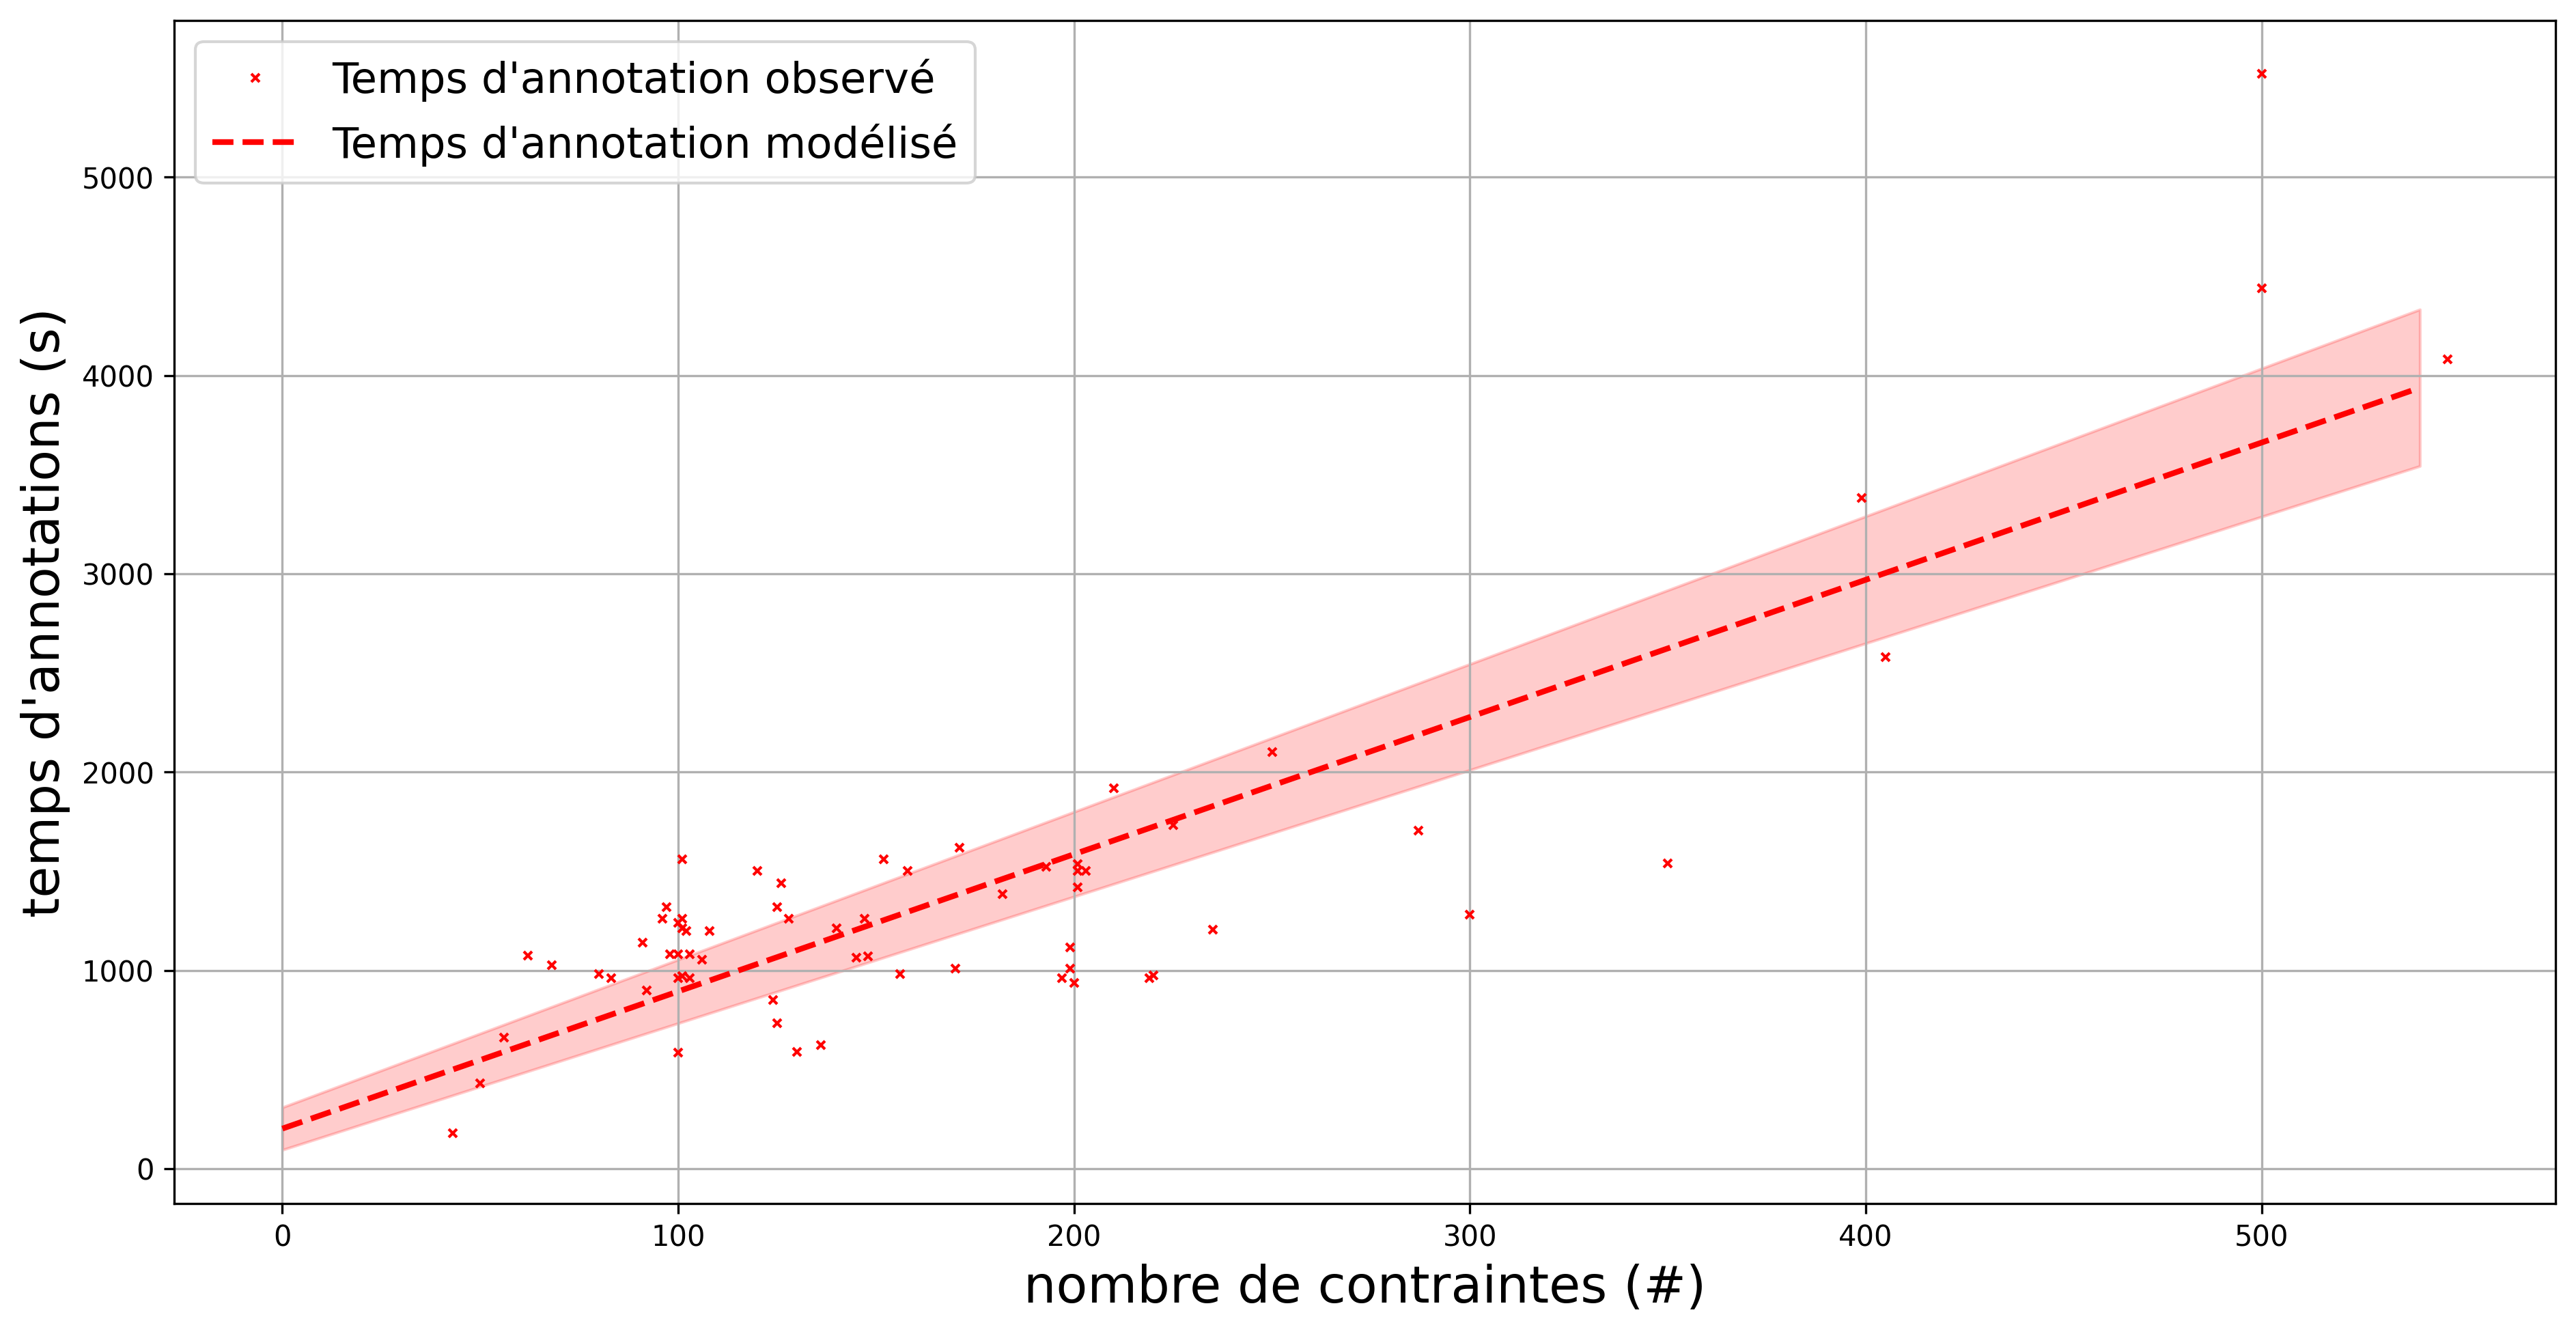
\includegraphics[width=0.95\textwidth]{figures/etude-temps-annotation-1-modelisation-temps}
				\caption{
					Estimation du temps nécessaire (en minutes) pour annoter un lot de contraintes.
				}
				\label{figure:4.3.1-ETUDE-COUTS-TEMPS-ANNOTATION-SIMULATION}
			\end{figure}
		
			% Étude de cas.
			En ce qui concerne l'évolution de la vitesse d'annotation au cours des sessions, aucune tendance significative n'a été identifiée. 
			La \textsc{Figure~\ref{figure:4.3.1-ETUDE-COUTS-TEMPS-ANNOTATION-EXEMPLE}} représente l'évolution de vitesse d'annotation pour quatre opérateurs (les deux plus rapides et les deux plus lents).
			Ces données sont l'objet d'une étude de cas dans la discussion ci-dessous.
			%
			\begin{figure}[!htb]
				\centering
				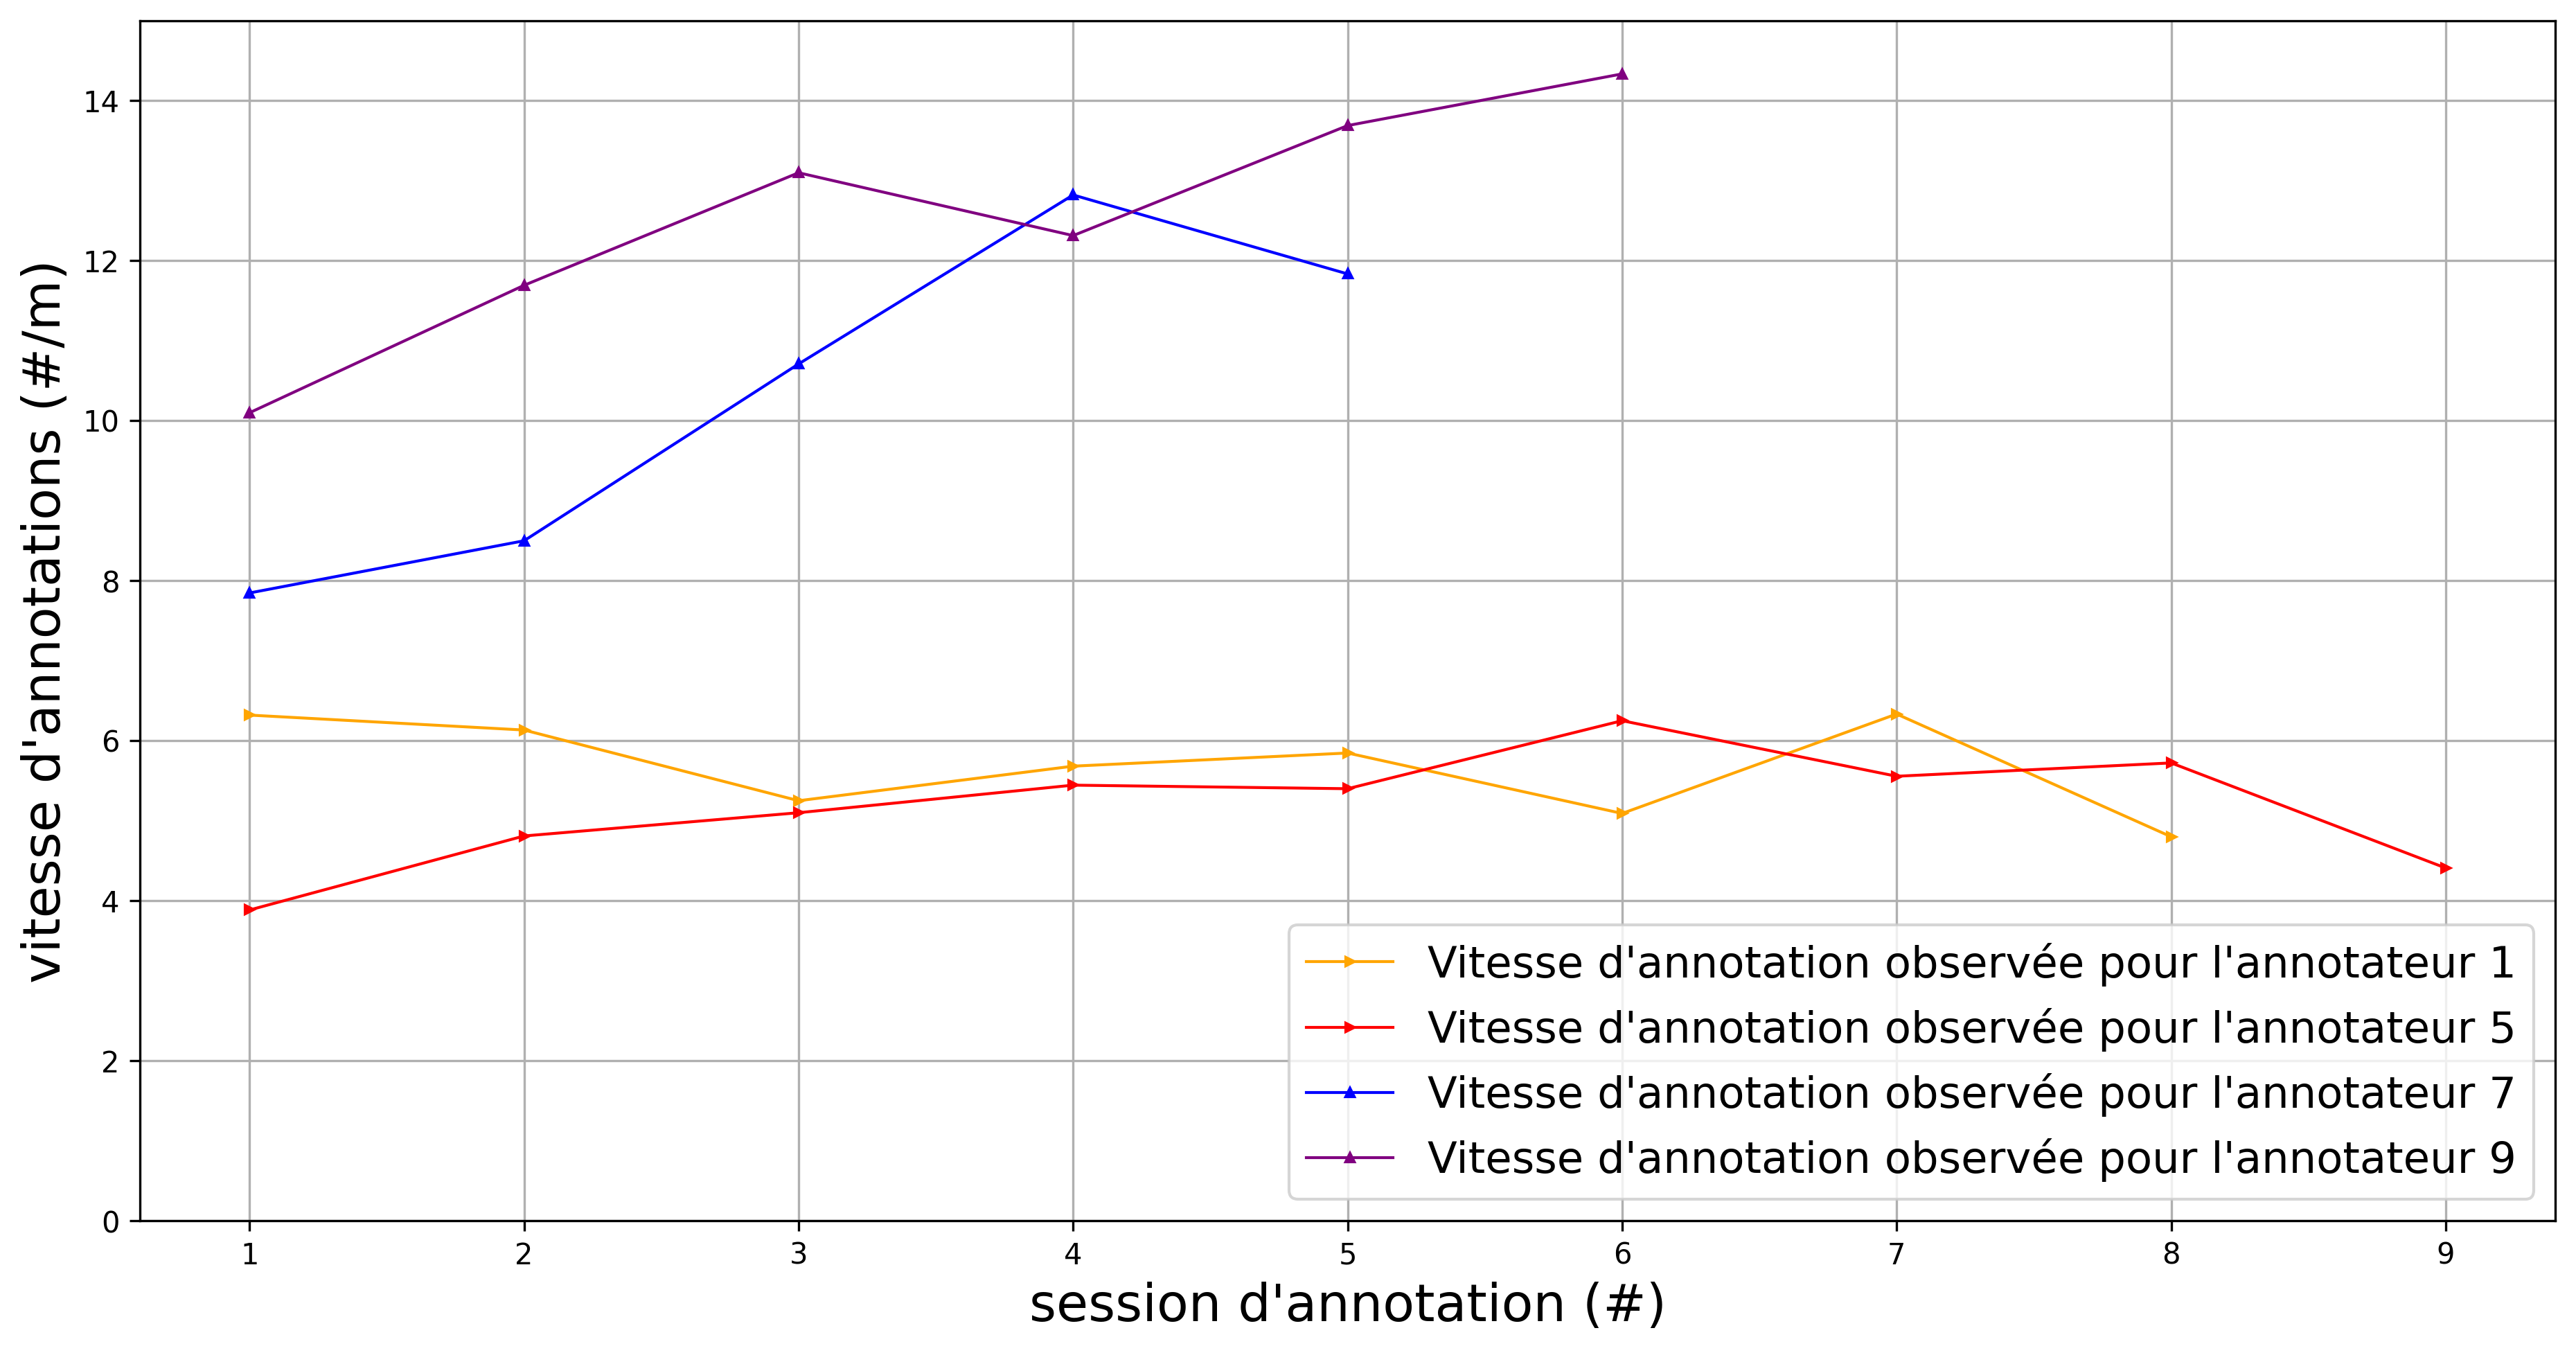
\includegraphics[width=0.95\textwidth]{figures/etude-temps-annotation-3-etude-de-cas}
				\caption{
					Étude de cas d'évolution de la vitesse d'annotation de contraintes (en contraintes par minutes) en fonction des différentes sessions d'annotations.
				}
				\label{figure:4.3.1-ETUDE-COUTS-TEMPS-ANNOTATION-EXEMPLE}
			\end{figure}

		%%% Discussion.
		\subsubsection{Discussion}

		
		% Généralités sur la modélisation du temps d'annotation sur une session.
		L'étude réalisée avec $14$ annotateurs sur des lots de $1~000$ contraintes a permis d'estimer à $7.8 \cdot \texttt{batch\_size}$ le temps nécessaire (en secondes) pour annoter un lot de contraintes (cf. \textsc{Figure~\ref{figure:4.3.1-ETUDE-COUTS-TEMPS-ANNOTATION-SIMULATION}}).
		
		% Compliqué de comparer ...
		\begin{leftBarAuthorOpinion}
			Avant poursuivre la discussion, il est nécessaire de préciser qu'il est difficile de comparer ces résultats.
			% Forte disparité des mesures.
			D'une part, il y a une forte disparité des mesures, et il est idyllique de penser qu'une étude sur $14$ annotateurs peut représenter la diversité du comportement humain sur une tâche aussi complexe que l'annotation de données textuelles.
			% Peu de repères concrets.
			D'autre part, il y a un manque de repères concrets dans la littérature scientifique, entre autres à cause des nombreux facteurs intervenant dans une tâche d'annotation (\textit{objectifs à réaliser, données à manipuler, nombre de choix proposés à l'opérateur, complexité sémantique des données, des compétences de l'opérateur, fréquence d'exécution de la tâche, ...}), mais aussi en raison du manque d'intérêt à l'analyse du temps nécessaire au profit de l'analyse de la cohérence et de la qualité intra- ou inter-annotateur (\cite{baledent:2022:complexite-annotation-manuelle}).
			% Diversité des données.
			De plus, les résultats peuvent différer en fonction des contraintes à caractériser : on peut supposer que des couples de données très similaires ou très différentes sont simples à annoter, mais que des données plus ambiguës peuvent nécessiter davantage de temps pour être intégrées et étiquetées.
			
			% Angle d'attaque.
			Pour pallier ce problème, nous proposons confronter nos estimations à des mesures réalisées sur des tâches n'ayant pas le même objectif mais dont la complexité est comparable.
			Cette approche, bien qu'un peu rudimentaire, nous permettra ainsi de discuter des ordres de grandeurs à manipuler.
		\end{leftBarAuthorOpinion}
		
		
		%%% A. Analyse de l'annotation d'une contraintes.
		\paragraph{Analyse de l'annotation d'une contraintes.}
		
			% Avantage 1: 8 secondes, c'est acceptable.
			En premier lieu, nous voulions confirmer que l'annotation de contraintes est une tâche intuitive dont la durée est est caractéristique d'un mécanisme de réaction et non d'une réflexion.
			Pour ce faire, nous avons estimé la durée théorique d'une annotation à $7$ secondes par contrainte, comprenant les temps de lecture, d'analyse de la similitude et d'action de l'opérateur, et nous avons mesuré la durée d'annotation réelle à $7.8$ secondes par contrainte.
			Bien que l'écart constaté ($0.8$ seconde) soit compris dans les bornes d'approximation, cette différence n'est pas suffisamment insignifiante pour nous permettre d'exclure avec certitude la présence d'un mécanisme cognitif supplémentaire.
				
			% Avantage 2: Dans tous les cas, 8 secondes, c'est mieux que 17 secondes ou 40 secondes.
			Pour nous permettre de discuter du temps d'annotation mesuré et de son approximation théorique, nous utilisons utiliser plusieurs points de référence extraits de (\cite{snow-etal:2008:cheap-fast-it}).
			Dans cette étude, les auteurs délèguent quelques tâches d'annotation à \texttt{Amazon Mechanical Turk}\footnote{
				\texttt{Amazon Mechanical Turk} est une plateforme de travail collaboratif en ligne (\textit{crowdsourcing}) : nous avions évoqué leur fonctionnement, leur avantages et leurs inconvénients en \textsc{Section~\ref{section:2.3.2.C-DEFIS-ANNOTATION-ASPECT-COMPLEXITE-COUTS}}, notamment le risque de l'abandon de la qualité des annotations au profit de la quantité.
			} :
			
			\begin{enumerate}
				% Task 1: (Word Sense Disambiguation)
				\item Tâche de "\textit{désambiguïsation du sens des mots}" (\cite{pradhan-etal:2007:semeval2007-task-17}) :
				Elle consiste à catégoriser le contexte de phrases comportant le mot "\textit{président}" suivant $3$ options préformatées (\textit{dirigeant d'une entreprise, dirigeant des États Unis, dirigeant d'un autre pays}).
				Il y a $177$ phrases à labelliser par $10$ annotateurs, et la tâche a été réalisée en un total de $8.59$ heures, soit une moyenne de $17.5$ secondes par annotation.
				Nous utilisons ce point de repère car la tâche s'apparente à une annotation d'une tâche de classification ($3$ catégories).
				% Task 2: (Word Similarity)
				\item Tâche de "\textit{caractérisation de similitude des mots}" (\cite{miller-charles:1991:contextual-correlates-semantic}) :
				Elle consiste à ordonner des couples de mots du plus similaire au moins similaire en fonction de leur proximité sémantique afin de mettre en avant les meilleurs couples de synonymes.
				Il y a $30$ paires de synonymes à ordonner par $10$ annotateur, et la tâche a été réalisée en un total de $0.17$ heures, soit une moyenne de $2.0$ secondes par annotation.
				Nous utilisons ce point de repère car la tâche s'apparente à l'annotation de contraintes (\textit{laquelle de ces deux paires est la plus adéquate ?}) qui ne fait pas appel à un mécanisme de réflexion (\textit{peu de vocabulaire, similarité intrinsèque triviale entre deux mots}).
				% Task 3: (Recognizing Textual Entailment)
				\item Tâche de "\textit{reconnaissance de l'implication textuelle}" (\cite{dagan-etal:2005:pascal-recognising-textual}) :
				Elle consiste à confirmer ou infirmer si une phrase est la conséquence d'une autre (\textit{l'annotation est donc binaire}).
				Il y a $800$ paires de phrases à valider par $10$ annotateur, et la tâche a été réalisée en un total de $89.3$ heures, soit une moyenne de $40.2$ secondes par annotation.
				Nous utilisons ce point de repère car la tâche s'apparente à l'annotation de contraintes (\textit{est-ce que l'implication est vraie ?}) faisant intervenir un mécanisme de réflexion (\textit{comprendre une implication logique}).
			\end{enumerate}
			%
			% Comparaison à Task 1: (Word Sense Disambiguation).
			En utilisant la tâche de "\textit{désambiguïsation du sens des mots}" (1.), nous avons déjà un point de comparaison entre notre annotation de contraintes et une annotation classique de classes.
			Nous constatons une nette différence entre les deux approches ($7.8$ secondes par contrainte vs $17.5$ secondes par donnée), cela met en avant qu'une annotation de contraintes est plus rapide qu'une annotation par label.
			
			% Comparaison à Task 2: (Word Similarity).
			Ensuite, en utilisant la tâche de "\textit{caractérisation de similitude des mots}" (2.), nous pouvons confirmer que notre approximation théorique (faisant intervenir un traitement cognitif de $1$ seconde) semble adaptée pour représenter un mécanisme de l'ordre de la réaction.
			En effet, le coût très faible de la caractérisation d'une similarité entre deux mots ($2.0$ secondes par paire de mots) s'avère être en adéquation avec cette approximation ($2.5$ secondes par paire de phrases de taille $1$).
			
			% Comparaison à Task 3: (Recognizing Textual Entailment).
			Enfin, en utilisant la tâche de "\textit{reconnaissance de l'implication textuelle}" (3.), nous comparons deux annotations binaires dont une fait nettement appel à un mécanisme de réflexion (déduction logique dans une implication).
			Nous constatons une très nette différence entre les deux approches ($7.8$ secondes par contrainte vs $40.2$ secondes par implication), ce qui nous permet d'exclure la présence de mécanisme cognitif trop complexe.
	
			% Conclusion sur l'analyse de l'annotation d'une contraintes.
			\begin{leftBarSummary}
				Mettant bout à bout ces comparaisons, et en gardant à l'esprit que ces références restent approximatives, nous pouvons conclure que (1) \textbf{l'annotation de contraintes est une tâche plus rapide qu'une annotation par label} et que (2) \textbf{cette annotation binaire ne semble pas faire pas intervenir de traitement cognitif complexe} (\textit{c'est une piste à explorer plus en détails pour expliquer le gain de temps observé}).
			\end{leftBarSummary}
		
		
		%%% B. Analyse d'une session d'annotation de contraintes.
		\paragraph{Analyse d'une session d'annotation de contraintes.}
		
			% Ouverture 1: Autres analyses sans conclusions.
			Nous avons analysé l'évolution de la vitesse d'annotation au cours des sessions d'annotation, en espérant observer une accélération des annotations au fur et à mesure que l'annotateur s'habitue avec la tâche, ainsi qu'un effet de fatigue pour des sessions d'annotations trop longues.
			Cependant, aucune de nos analyses n'a montré de résultats significatifs (on peut constater la forte dispersion des résultats grâce à la \textsc{Figure~\ref{figure:4.3.1-ETUDE-COUTS-TEMPS-ANNOTATION-EXEMPLE}}).
			Nous ne pouvons donc pas conclure sur de telles tendances.
			
			\begin{leftBarAuthorOpinion}
				Nos intuitions initiales concernaient deux points :
				\begin{itemize}
					% Temps d'adaptation.
					\item la diminution du \textbf{temps d'adaptation} au cours de sessions d'annotations : au fur et à mesure qu'il annote, l'opérateur pourrait entrer plus facilement dans sa tâche, lui permettant d'atteindre plus rapidement sa vitesse de croisière et ainsi gagner en efficacité sur plusieurs sessions.
					D'après \cite{anderson:2013:architecture-cognition}, ce temps d'adaptation pourrait se définir en trois étapes : une phase déclarative (\textit{besoin d'instructions détaillées, exécution lente et avec erreurs}), une phase associative (\textit{quelques rappels clés suffisent pour retrouver les instructions, donc gain de vitesse}) et une phase autonome (\textit{les consignes sont acquises, donc exécution rapide et sans erreur}) ;
					% Effet de fatigue.
					\item l'intervention d'un \textbf{effet de fatigue} : si une session d'annotation dure trop longtemps, l'opérateur pourrait perdre en efficacité par manque de concentration et augmenter ses chances de faire des erreurs.
					D'après \cite{jones-etal:2015:demographic-occupational-predictors}, la fatigue est considérée comme un inconfort qui s'installe après une tâche excessive, et \cite{elkosantini-gien:2009:integration-human-behavioural} décrit cet état de fatigue par des capacités de travail réduites.
				\end{itemize}
				%
				Ces différentes intuitions ont aussi été remontées par les annotateurs de notre expériences, mais aucun effet significatif n'a pu être observé.
			\end{leftBarAuthorOpinion}
		
			% Ouverture 2: Remarque sur le nombre maximal moyen de contraintes à annoter.
			Par extension, nous ne pouvons pas non plus conclure sur la taille optimale d'échantillon de contraintes à sélectionner pour une session d'annotation.
			Dans nos précédentes études, nous avions arbitrairement fixé la taille de lot à $50$ pour bénéficier d'itérations brèves, permettant à l'algorithme de \textit{clustering} de l'améliorer régulièrement avec les dernières contraintes.
			Mais des petits lots d'annotation démultiplient le nombre d'itérations à réaliser, et donc le nombre d'algorithmes à exécuter.
			Il serait donc judicieux d'adapter le nombre d'annotations à réaliser pour d'améliorer l'expérience utilisateur en situation réelle de l'opérateur.
			Malheureusement, aucun repère significatif ne peut être déduit de nos résultats pour prédire la fin d'un temps d'adaptation ou le début d'un effet de fatigue.
			
			% Idées : nombre de contraintes moyen par session.
			Afin de proposer tout de même un ordre de grandeur de taille de lot, nous pouvons nous intéresser au nombre moyen de contraintes annotées lors des sessions réalisées par les opérateurs de notre expérience.
			Bien que ces informations n'ont pas été collectées initialement à cette fin, on peut supposer que les opérateurs ont interrompu leur session pour se reposer (\textit{par fatigue, ennui, agacement, ...}) ou répondre à une autre sollicitation (\textit{intervention d'un collègue, mail important, pause café, ...})
			Après un entretien avec les opérateurs de notre expérience, il semble y avoir deux possibilités : soit l'opérateur ne se fixait pas d'objectif et s'arrêtait par fatigue ; soit il se fixait un objectif (\textit{de nombre ou de durée}), mais adaptait son prochain objectif en fonction de la fatigue ressentie en fin de session.
			Dans les deux cas, nous pouvons faire l'hypothèse que le nombre moyen d'annotation par session tend à représenter une borne supérieure de la taille maximale d'un lot à considérer pour ne pas entamer l'effet de fatigue.
			Sur l'expérience réalisée, cette moyenne est de $170.70$ contraintes annotées par session (écart-type: $106.37$, erreur standard: $13.19$).
			En prenant en compte une marge d'erreur pour minimiser ce résultat, nous retenons $150$ contraintes comme seuil à ne pas dépasser.
			
			% Conclusion sur l'analyse d'une session d'annotation de contraintes.
			\begin{leftBarSummary}
				Pour une session d'annotation, \textbf{nous conseillons une taille d'échantillon entre $50$ et $150$ contraintes}.
				Attention aux échantillons trop petits qui multiplient le nombre d'itérations à réaliser ;
				Attention aussi aux échantillons trop gros qui peuvent introduire un effet de fatigue chez l'opérateur et casser la dynamique d'interactions avec la machine.
				La discussion finale de ce chapitre affinera cette fourchette grâce à une vue d'ensemble sur les coûts de la méthode.
			\end{leftBarSummary}
			

		%%% C. Analyse des fonctionnalités de l'application d'annotation
		\paragraph{Analyse des fonctionnalités de l'application d'annotation.}
		
			% Ouverture 3: Autres remontées applicatives.
			Pour finir cette discussion, nous nous intéressons à l'utilisation du logiciel par nos opérateurs au cours de cette étude.
			En effet, il est logique de penser que la conception de l'application et les fonctionnalités qu'elle dispose peut grandement impacter l'expérience utilisateur de notre méthodologie de \textit{clustering} itératif.
			Un entretien avec les opérateurs a permis de remonter plusieurs pistes d'amélioration sur son ergonomie.
			
			% Idées 1: Données non prétraitées.
			Un premier point concerne l'affichage des textes d'une contraintes.
			Comme montré en \textsc{Figure~\ref{figure:4.3.1-ETUDE-COUTS-TEMPS-ANNOTATION-APPLICATION-ANNOTATION}}, nous avions choisi d'affichée des données normalisées à l'écran pour masquer le bruit provoqué par les accents, les majuscules, la ponctuation.
			Bien que cette fonctionnalité peut servir pour des textes bruts (issues de conversation clients ou de forum par exemple), cela a plutôt nuit à la compréhension des données par les opérateurs.
			Nous avons donc envisager de laisser la données brutes à disposition, dans une infobulle ou grâce à une option permettant d'interchanger le format des données.
			
			% Idée 2: Ordonner les données.
			Une seconde proposition concerne l'ordre des contraintes à annoter.
			Nous pouvons facilement admettre que la compréhension rapide d'un grand nombre de texte est un tâche pénible.
			Pour soulager les opérateurs et limiter le nombre de transitions, nous avons trier les contraintes par ordre alphabétique.
			Ainsi, toutes les contraintes associées à une même donnée peuvent être traitées à la suite.
			Cette solution permet de limiter le nombre de changement de contexte et peut faciliter la caractérisation d'une similitude en analysant à la chaîne plusieurs données du même type.
			À cet effet, une option e tri à été ajouté sur la liste de contraintes à traiter (cf. \textsc{Figure~\ref{figure:4.3.1-ETUDE-COUTS-TEMPS-ANNOTATION-APPLICATION-LISTE-CONTRAINTES}}).
			
			% Idée 3: Annotation multi-contraintes.
			Enfin, une dernière idée concerne l'affichage des données à annoter.
			Nous avions jusqu'à présent considérer l'annotation entre deux données (cf. \textsc{Figure~\ref{figure:4.3.1-ETUDE-COUTS-TEMPS-ANNOTATION-APPLICATION-ANNOTATION}}), mais il peut être judicieux d'afficher plusieurs données à caractériser simultanément.
			Une telle fonctionnalité permettrait ainsi de regrouper rapidement un grand nombre de données similaires ou de distinguer avec moins d'ambiguïté certaines données en s'appuyant sur leur voisinage.
			
			\begin{leftBarInformation}
				Ces différentes évolutions sont en cours d'analyse ou ont déjà été intégrées dans l'application que nous proposons (\cite{schild-etal:2022:cognitivefactory-interactiveclusteringgui}).
			\end{leftBarInformation}
	

	%%%
	%%% Subsection 4.3.2: Étude du temps de calcul nécessaire aux algorithmes implémentés en chronométrant des exécutions dans différentes situations
	%%%
	\subsection{Étude du temps de calcul nécessaire aux algorithmes implémentés en chronométrant des exécutions dans différentes situations}
	\label{section:4.3.2-ETUDE-COUTS-TEMPS-CALCUL}
		
		% Transition.
		Maintenant que nous avons pu modéliser le temps nécessaire à un expert pour annoter un lot de contraintes, nous nous intéressons au temps nécessaire à la machine pour interpréter ces annotations et proposer une nouvelle segmentation des données.
		
		% Complexité de la tâche.
		Comme les différents algorithmes employés manipulent des contraintes sur les données, l'estimation théorique du temps d'exécution par l'analyse de la complexité ne semble pas fiable : en effet, quelques contraintes bien placées peuvent suffire à simplifier le fonctionnement d'un algorithme de \textit{clustering} alors qu'une grande quantité de contraintes mal placées vont au contraire le pénaliser.
		% Objectif de l'expérience.
		Nous préférons donc une approche empirique en chronométrant plusieurs exécutions isolées des algorithmes intervenant dans notre implémentation du \textit{clustering} interactif et en évaluant l'importance de leurs différents arguments d'entrée (la taille du jeu de données, le nombre de clusters et le nombre de contraintes annotées, ...).
		Nous profitons aussi de ces modélisations du temps de calcul pour confirmer le choix de paramétrage réalisé lors de l'étude d'efficience en \textsc{Section~\ref{section:4.2-HYPOTHESE-EFFICIENCE}}, et ainsi faire un compromis entre l'algorithme le plus efficient et l'algorithme le plus rapide.
	
		%%% Protocole expérimental.
		\subsubsection{Protocole expérimental}
			
			% Pseudo-code.
			Pour résumer le protocole expérimental que nous décrivons ci-dessous, vous pouvez vous référer aux pseudo-code décrit dans \textsc{Algorithme~\ref{algorithm:4.3.2-ETUDE-COUTS-TEMPS-CALCUL-PROTOCOLE}}.
			
			\begin{algorithm}
				\KwData{jeux de données annotées (vérités terrains) de tailles différentes}
				\KwIn{combinaisons d'algorithmes et de paramètres à tester}
				%
				\ForEach{combinaison d'algorithmes et de paramètres à tester}{
					\textbf{initialisation (données)}: récupérer ou générer le jeu de données \;
					\textbf{initialisation (contraintes)}: créer une liste vide de contraintes \;
					\If{estimation de la tâche de \textbf{prétraitement}}{
						\textbf{chronomètre}: \textbf{START} \;
						\textbf{prétraitement (à étudier)}: supprimer le bruit dans les données \;
						\textbf{chronomètre}: \textbf{STOP} \;
					}
					\ElseIf {estimation de la tâche de \textbf{vectorisation}}{
						\textbf{prétraitement}: supprimer le bruit dans les données avec \texttt{prep.simple} \;
						\textbf{chronomètre}: \textbf{START} \;
						\textbf{vectorisation (à étudier)}: transformer les données en vecteurs \;
						\textbf{chronomètre}: \textbf{STOP} \;
					}
					\ElseIf {estimation de la tâche de \textbf{clustering}}{
						\textbf{prétraitement}: supprimer le bruit dans les données avec \texttt{prep.simple} \;
						\textbf{vectorisation}: transformer les données en vecteurs avec \texttt{vect.tfidf} \;
						\textbf{échantillonnage initial}: sélectionner des contraintes avec \texttt{samp.rand.full} \;
						\textbf{simulation d'annotation}: déterminer les contraintes avec la vérité terrain \;
						\textbf{intégration}: ajouter les nouvelles contraintes au gestionnaire de contraintes \;
						\textbf{chronomètre}: \textbf{START} \;
						\textbf{clustering (à étudier)}: regrouper les données par similarité \;
						\textbf{chronomètre}: \textbf{STOP} \;
					}
					\ElseIf {estimation de la tâche d'\textbf{échantillonnage}}{
						\textbf{prétraitement}: supprimer le bruit dans les données avec \texttt{prep.simple} \;
						\textbf{vectorisation}: transformer les données en vecteurs avec \texttt{vect.tfidf} \;
						\textbf{échantillonnage initial}: sélectionner des contraintes avec \texttt{samp.rand.full} \;
						\textbf{simulation d'annotation}: déterminer les contraintes avec la vérité terrain \;
						\textbf{intégration}: ajouter les nouvelles contraintes au gestionnaire de contraintes \;
						\textbf{clustering initial}: regrouper les données avec \texttt{clust.kmeans.cop} \;
						\textbf{chronomètre}: \textbf{START} \;
						\textbf{échantillonnage (à étudier)}: sélectionner de nouvelles contraintes à annoter \;
						\textbf{chronomètre}: \textbf{STOP} \;
					}
				}
				\ForEach{algorithme à modéliser}{
					\textbf{cadrage}: définir les facteurs et les interactions intervenant dans la modélisation \;
					\textbf{simplification}: restreindre la modélisation aux facteurs les plus corrélés \;
					\textbf{analyse}: modéliser le temps d'exécution avec les facteurs retenus \;
				}
				%
				\KwResult{modélisation du temps d'exécution des différents algorithmes}
				%
				\caption{\textit{
					Description en pseudo-code du protocole expérimental de l'étude du temps d'exécution des algorithmes du \textit{clustering} interactif.
				}}
				\label{algorithm:4.3.2-ETUDE-COUTS-TEMPS-CALCUL-PROTOCOLE}
			\end{algorithm}
			
			% Description de la vérité terrain.
			Nous utilisons le jeu de données \texttt{Bank Cards (v2.0.0)} comme référence pour cette expérience : ce dernier traite des demandes les plus fréquentes des clients en ce qui concerne la gestion de leur carte bancaire.
			Il est composé de $1~000$ questions rédigées en français et réparties en $10$ classes (\texttt{perte ou vol de carte}, \texttt{carte avalée}, \texttt{commande de carte}, ...).
			Pour plus de détails, consultez l'annexe~\ref{annex:A.1-DATASET-BANK-CARDS}.
			Cependant, un seul jeu de données ne nous permet pas d'analyser l'impact du nombre de données sur le temps d'exécution des algorithmes.
			Pour utiliser facilement plusieurs jeux de données de tailles différentes tout en maîtrisant leur contenu, nous avons donc dupliqué aléatoirement des données issues du jeu de référence en y insérant des fautes de frappes.
			
			% Remarques.
			\begin{leftBarWarning}
				Dans le cadre de cette étude, nous faisons l'hypothèse que cette création artificielle de données n'a pas d'impact majeur sur le temps d'exécution des différents algorithmes.
			\end{leftBarWarning}
			
			% Description des tâches, des algorithmes et des contextes.
			À l'aide de ces données, nous lançons plusieurs exécutions de chaque algorithme de notre implémentation du \textit{clustering} interactif (cf. \textsc{Section~\ref{section:3.3-DESCRIPTION-IMPLEMENTATION}}) avec différentes variations de contexte d'utilisation.
			Cela comprend les tâches, algorithmes et contextes d'utilisation suivants :
			\begin{enumerate}
				% Prétraitement.
				\item le \textbf{prétraitement} des données...
					\begin{itemize}
						\item avec les algorithmes suivants : \textbf{simple} (noté \texttt{prep.simple}), \textbf{avec lemmatisation} (noté \texttt{prep.lemma}) et \textbf{avec filtres} (noté \texttt{prep.filter}) ;
						\item avec les contextes d'utilisation suivants : \textbf{nombre de données} (variant de $1~000$ à $5~000$ par pas de $1~000$, noté $\texttt{dataset\_size}$) ;
					\end{itemize}
				% Vectorisation.
				\item la \textbf{vectorisation} des données...
					\begin{itemize}
						\item avec les algorithmes suivants : \textbf{TF-IDF} (noté \texttt{vect.tfidf}) et \textbf{SpaCy} (noté \texttt{vect.frcorenewsmd}) ;
						\item avec les contextes d'utilisation suivants : \textbf{nombre de données} (variant de $1~000$ à $5~000$ par pas de $1~000$, noté $\texttt{dataset\_size}$) ;
						\item précédé par un prétraitement \textbf{simple} ;
					\end{itemize}
				% Clustering.
				\item le \textbf{\textit{clustering} sous contraintes} des données...
					\begin{itemize}
						\item avec les algorithmes suivants : \textbf{KMeans} (modèle \textit{COP} noté \texttt{clust.kmeans.cop}), \textbf{Hiérarchique} (lien \textit{single} noté \texttt{clust.hier.sing} ; lien \textit{complete} noté \texttt{clust.hier.comp} ; lien \textit{average} noté \texttt{clust.hier.avg} ; lien \textit{ward} noté \texttt{clust.hier.ward}) et \textbf{Spectral} (modèle \textit{SPEC} noté \texttt{clust.spec}) ;
						\item avec les contextes d'utilisation suivants : \textbf{nombre de données} (variant de $1~000$ à $5~000$ par pas de $1~000$, noté $\texttt{dataset\_size}$), le \textbf{nombre de contraintes annotés} (variant de $0$ à $5~000$ par pas de $500$, noté $\texttt{previous\_nb\_constraints}$) et le \textbf{nombre de \textit{clusters} à trouver} (variant de $5$ à $50$ par pas de $5$, noté $\texttt{algorithm\_nb\_clusters}$) ;
						\item précédé par un prétraitement \textbf{simple} et une vectorisation \textbf{TF-IDF} et un échantillonnage initial \textbf{purement aléatoire} ;
					\end{itemize}
				% Sampling.
				\item l'\textbf{échantillonnage} des contraintes à annoter...
					\begin{itemize}
						\item avec les algorithmes suivants : \textbf{purement aléatoire} (noté \texttt{samp.random.full}), \textbf{pseudo-aléatoire} (noté \texttt{samp.random.same}), \textbf{même cluster et étant les plus éloignées} (noté \texttt{samp.farhtest.same}) et \textbf{clusters différents et étant les plus proches} (noté \texttt{samp.closest.diff}) ;
						\item avec les contextes d'utilisation suivants : \textbf{nombre de données} (variant de $1~000$ à $5~000$ par pas de $1~000$, noté $\texttt{dataset\_size}$), le \textbf{nombre de contraintes annotés} (variant de $0$ à $5~000$ par pas de $500$, noté $\texttt{previous\_nb\_constraints}$), le \textbf{nombre de \textit{clusters} existant} (variant de $10$ à $50$ par pas de $10$, noté $\texttt{previous\_nb\_clusters}$) et le \textbf{nombre de contraintes à sélectionner} (variant de $50$ à $250$ par pas de $50$, noté $\texttt{algorithm\_nb\_constraints}$) ;
						\item précédé par un prétraitement \textbf{simple}, une vectorisation \textbf{TF-IDF}, un \textit{clustering} initial \textbf{KMeans} (modèle \textit{COP}) et un échantillonnage initial \textbf{purement aléatoire} ;
					\end{itemize}
			\end{enumerate}
			
			Il y a donc $8~825$ combinaisons d'algorithmes (\texttt{15} pour le prétraitement, $10$ pour la vectorisation, $3~330$ pour le \textit{clustering}, $5~550$ pour l'échantillonnage), et chaque combinaison est répétée $5$ fois pour contrer les aléas statistiques des exécutions.
			De plus, chaque jeu de données est généré $5$ fois pour contrer les aléas statistiques de création, donc il y a $220~625$ exécutions d'algorithmes ($375$ pour le prétraitement, $250$ pour la vectorisation, $82~500$ pour le \textit{clustering}, $137~500$ pour l'échantillonnage).
			
			% Description de la modélisation.
			Sur la base de ces mesures, nous cherchons à modéliser le temps d'exécution de chaque algorithme en fonction de son contexte d'utilisation (dépendant de ses arguments d'entrée), et les interactions doubles entre paramètres sont envisagées.
			Afin de réduire la complexité des modélisations, nous ordonnons les interactions de facteurs possibles en fonction de leur corrélation avec le temps mesuré (la corrélation \texttt{r} de \textit{Pearson} (\cite{kirch:2008:pearson-correlation-coefficient}) est utilisée) et nous nous limitons aux variables responsables d'un maximum de la variance des mesures (la méthode d'\textit{Elbow} (\cite{thorndike:1953:who-belongs-family}) est utilisée pour choisir les facteurs pertinents).
			Sur cette base, nous entraînons un modèle linéaire généralisé (\textit{GLM}, cf. \cite{nelder-wedderburn:1972:generalized-linear-models}) pour représenter le temps d'exécution moyen de l'algorithme : ce modèle sera caractérisé par le coefficient de détermination généralisé \texttt{R²} de \textit{Cox et Snel} (\cite{diamond-etal:1990:analysis-binary-data}), la log-vraisemblance \texttt{llf} (\cite{edwards:1992:likelihood}) et la log-vraisemblance \texttt{llf\_null} du modèle \textit{null}.
			Pour finir, nous discutons des valeurs des coefficients obtenus sur l'impact du temps d'exécution.
			
			% Référence scripts.
			\begin{leftBarInformation}
				Les scripts de l'expérience, réalisés avec des \textit{notebooks} Python (\cite{van-rossum-drake:2009:python-reference-manual}), sont disponibles dans un dossier dédié de~\cite{schild:2021:cognitivefactory-interactiveclusteringcomparativestudy}.
				Nous utilisons entre autres les librairies \texttt{datetime} et \texttt{statsmodels} (\cite{seabold-perktold:2010:statsmodels-econometric-statistical}).
			\end{leftBarInformation}

		%%% Résultats.
		\subsubsection{Résultats obtenus}
				
			%%% Prétraitements
			
			% Première analyse.
			En ce qui concerne la tâche de \textbf{prétraitement}, une première analyse montre que les modélisations des trois implémentations sont similaires (\texttt{p-valeur}: $> 0.980$). Nous faisons donc une seule modélisation.
			
			% Modélisation du temps de calcul (prep.simple + prep.lemma + prep.filter).
			Pour les algorithmes de prétraitements (\texttt{prep.simple}, \texttt{prep.lemma} et \texttt{prep.filter}), l'analyse de la corrélation des facteurs avec les mesures de temps d'exécution indique qu'une modélisation minimale et suffisante peut être réalisée à partir du facteur $\texttt{dataset\_size}$ (\texttt{r}: $0.997$).
			Le modèle linéaire généralisé retenu (\texttt{R²}: $> 0.999$, \texttt{llf}: $-432.43$, \texttt{llf\_null}: $-1~353.98$) nous permet de déduire l'équation suivante :
			%
			\begin{equation}
				\texttt{computation\_time}(\texttt{prep})~[s]~
				\propto~6.55 \cdot 10^{-3} \cdot \texttt{dataset\_size}
			\end{equation}
			
			% Affichage du temps de calcul.
			La \textsc{Figure~\ref{figure:4.3.2-ETUDE-COUTS-TEMPS-CALCUL-MODELISATION-PREPROCESSING}} représente cette modélisation du temps de calcul des algorithmes de prétraitements en comparaison avec les mesures réalisées lors de l'expérience.
			\newline
			%
			\begin{figure}[!htb]
				\centering
				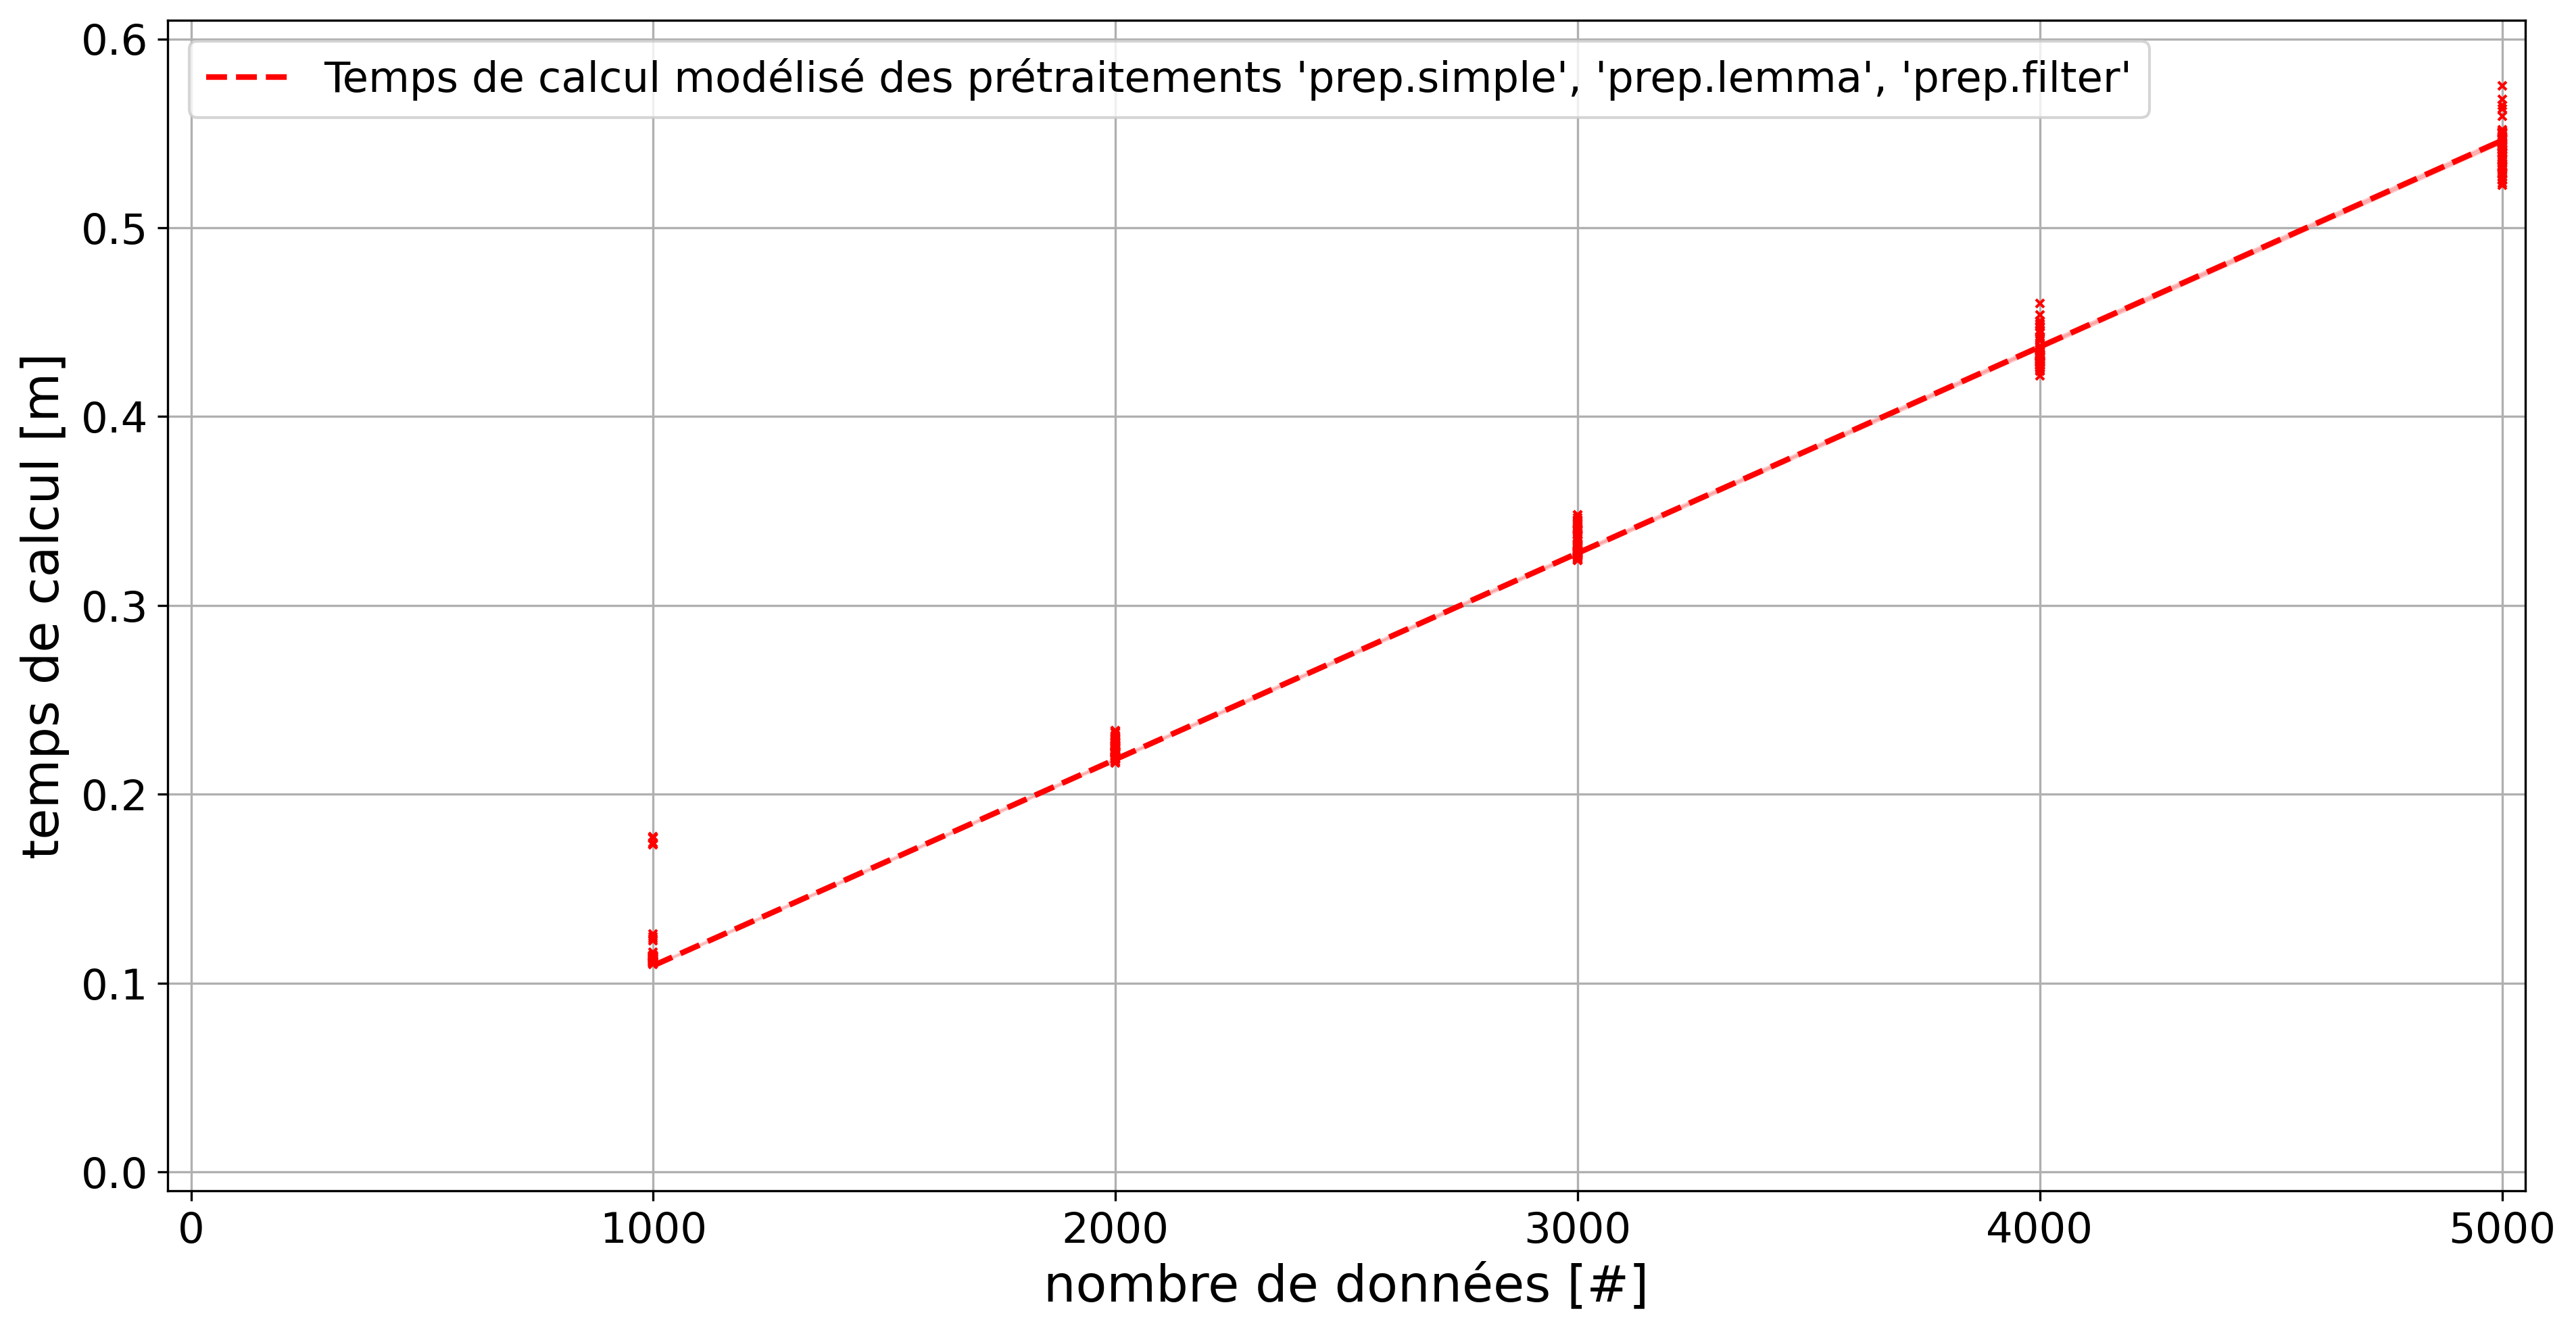
\includegraphics[width=0.95\textwidth]{figures/etude-temps-calcul-modelisation-1prep}
				\caption{
					Estimation du temps nécessaire (en minutes) pour effectuer une tâche de \textbf{prétraitement} en fonction du nombre de données à traiter. Les paramétrages \texttt{prep.simple}, \texttt{prep.lemma} et \texttt{prep.filter} ayant des temps de calculs similaires, leurs modélisations n'ont pas été séparées.
				}
				\label{figure:4.3.2-ETUDE-COUTS-TEMPS-CALCUL-MODELISATION-PREPROCESSING}
			\end{figure}
			
			%%% Vectorization
			
			% Première analyse.
			En ce qui concerne la tâche de \textbf{vectorisation}, une première analyse montre que les modélisations des deux implémentations sont différentiables (\texttt{p-valeur}: $< 10^{-3}$). Nous faisons donc une modélisation par algorithme.
		
			% Modélisation du temps de calcul (vect.tfidf).
			Pour les algorithmes de vectorisation \texttt{vect.tfidf}, l'analyse de la corrélation des facteurs avec les mesures de temps d'exécution indique qu'une modélisation minimale et suffisante peut être réalisée à partir du facteur $\texttt{dataset\_size}$ (\texttt{r}: $0.977$).
			Le modèle linéaire généralisé retenu (\texttt{R²}: $> 0.999$, \texttt{llf}: $259.89$, \texttt{llf\_null}: $70.04$) nous permet de déduire l'équation suivante :
			%
			\begin{equation}
				\texttt{computation\_time}(\texttt{vect.tfidf})~[s]~
				\propto~9.16 \cdot 10^{-5} \cdot \texttt{dataset\_size}
			\end{equation}
			
			% Modélisation du temps de calcul (vect.frcorenewsmd).
			Pour les algorithmes de vectorisation \texttt{vect.frcorenewsmd}, l'analyse de la corrélation des facteurs avec les mesures de temps d'exécution indique qu'une modélisation minimale et suffisante peut être réalisée à partir du facteur $\texttt{dataset\_size}$ (\texttt{r}: $0.983$).
			Le modèle linéaire généralisé retenu (\texttt{R²}: $> 0.999$, \texttt{llf}: $-214.44$, \texttt{llf\_null}: $-399.39$) nous permet de déduire l'équation suivante :
			%
			\begin{equation}
				\texttt{computation\_time}(\texttt{vect.frcorenewsmd})~[s]~
				\propto~4.62 \cdot 10^{-3} \cdot \texttt{dataset\_size}
			\end{equation}
			
			% Affichage du temps de calcul.
			La \textsc{Figure~\ref{figure:4.3.2-ETUDE-COUTS-TEMPS-CALCUL-MODELISATION-VECTORIZATION}} représente ces modélisations de temps de calcul des algorithmes de vectorisation en comparaison avec les mesures réalisées lors de l'expérience.
			\newline
			%
			\begin{figure}[!htb]
				\centering
				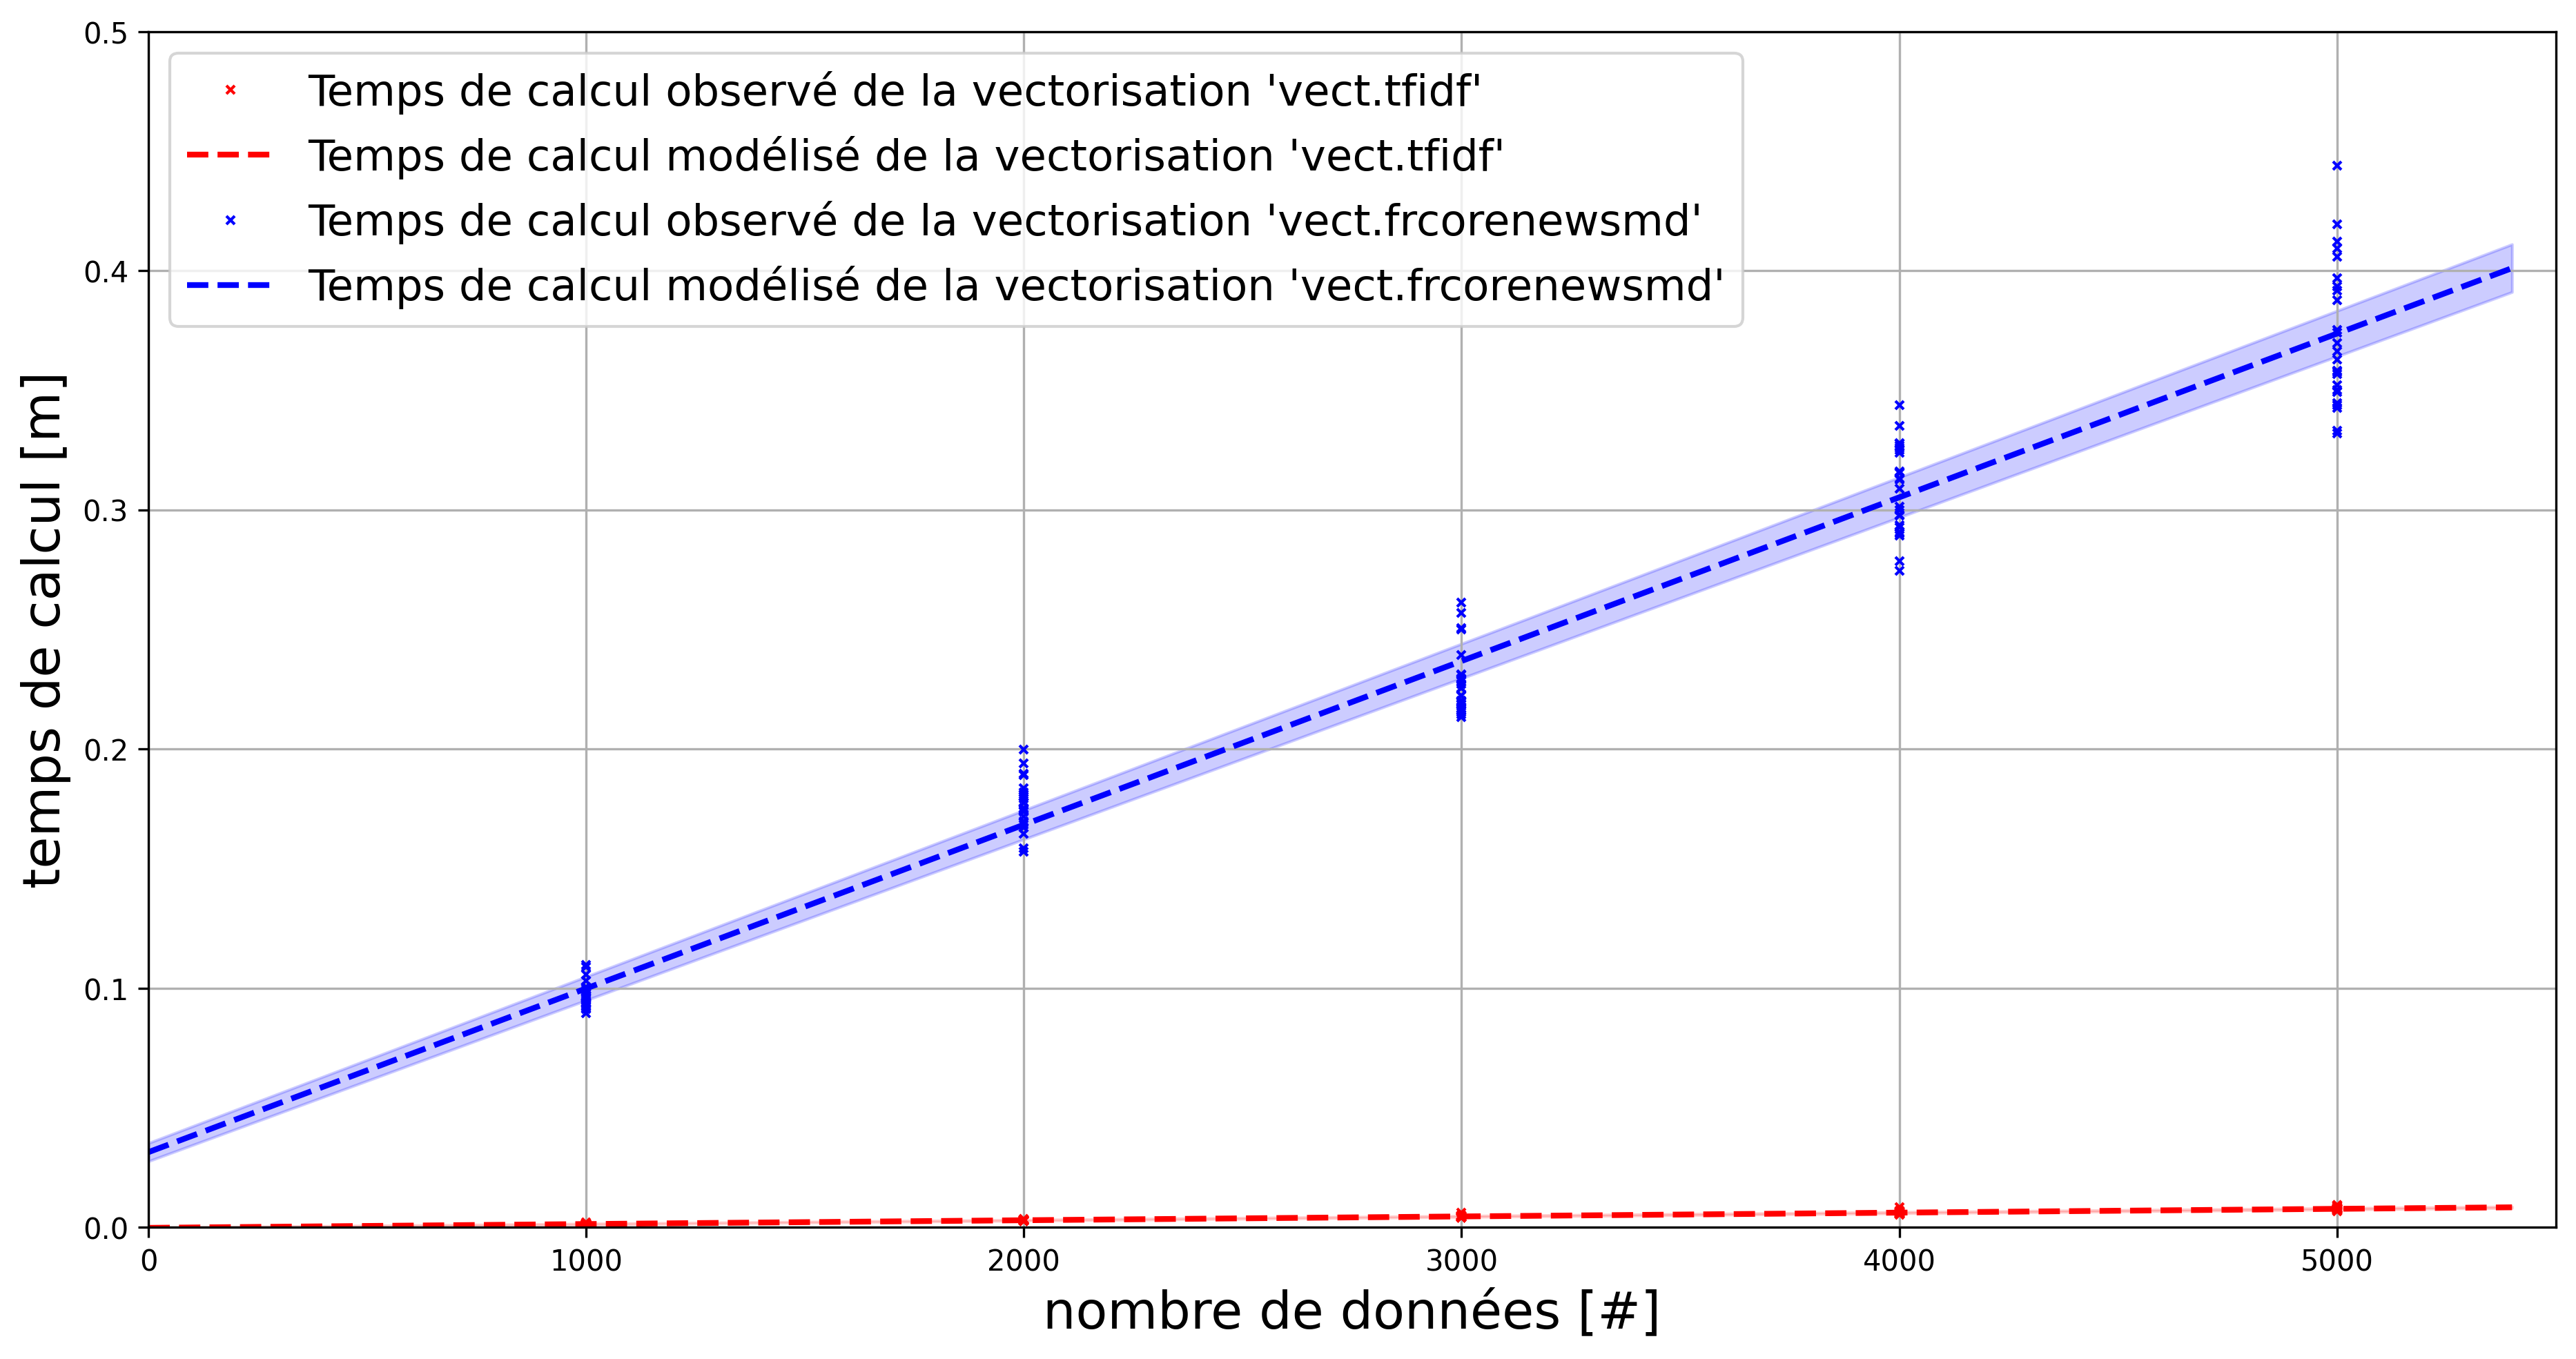
\includegraphics[width=0.95\textwidth]{figures/etude-temps-calcul-modelisation-2vect}
				\caption{
					Estimation du temps nécessaire (en minutes) pour effectuer une tâche de \textbf{vectorisation} en fonction du nombre de données à traiter.
				}
				\label{figure:4.3.2-ETUDE-COUTS-TEMPS-CALCUL-MODELISATION-VECTORIZATION}
			\end{figure}
			
			%%% Clustering
			
			% Première analyse.
			En ce qui concerne la tâche de \textbf{\textit{clustering} sous contraintes}, une première analyse montre que les modélisations des six implémentations sont différentiables (\texttt{p-valeur}: $<$ \texttt{$10^{-3}$}). Nous faisons donc une modélisation par algorithme.
			
			% Remarques: hiérarchique trop long.
			\begin{leftBarWarning}
				Plusieurs exécutions des algorithmes de type \textit{hiérarchique} ont été annulées pour les jeux données de tailles supérieures à $4~000$ car la durée excédé plusieurs heures.
				Nous limitons donc l'analyse de \texttt{clust.hier.sing}, \texttt{clust.hier.comp}, \texttt{clust.hier.avg} et \texttt{clust.hier.ward} aux tailles de $1~000$ à $3~000$.
			\end{leftBarWarning}
			
			% Modélisation du temps de calcul (clust.kmeans.cop).
			Pour les algorithmes du \textit{clustering} sous contraintes \texttt{clust.kmeans.cop}, l'analyse de la corrélation des facteurs avec les mesures de temps d'exécution indique qu'une modélisation minimale et suffisante peut être réalisée à partir du facteur $\texttt{dataset\_size}$ (\texttt{r}: $0.837$).
			Le second facteur le plus corrélé (mais non retenu) est l'interaction $\texttt{dataset\_size}^{\textbf{2}} \cdot \texttt{algorithm\_nb\_clusters}$ (\texttt{r}: $0.545$).
			Le modèle linéaire généralisé retenu (\texttt{R²}: $0.802$, \texttt{llf}: $-9.37 \cdot 10^{4}$, \texttt{llf\_null}: $-1.00 \cdot 10^{5}$) nous permet de déduire l'équation suivante :
			%
			\begin{equation}
				\texttt{computation\_time}(\texttt{clust.kmeans.cop})~[s]~
				\propto~1.45 \cdot 10^{-1} \cdot \texttt{dataset\_size}
			\end{equation}
			
			% Modélisation du temps de calcul (clust.hier.sing).
			Pour les algorithmes du \textit{clustering} sous contraintes \texttt{clust.hier.sing}, l'analyse de la corrélation des facteurs avec les mesures de temps d'exécution indique qu'une modélisation minimale et suffisante peut être réalisée à partir du facteur $\texttt{dataset\_size}^{\textbf{2}}$ (\texttt{r}: $0.940$).
			Le second facteur le plus corrélé (mais non retenu) est l'interaction $\texttt{dataset\_size}^{\textbf{2}} \cdot \texttt{algorithm\_nb\_clusters}$ (\texttt{r}: $0.729$).
			Le modèle linéaire généralisé retenu (\texttt{R²}: $0.987$, \texttt{llf}: $-5.54 \cdot 10^{4}$, \texttt{llf\_null}: $-6.10 \cdot 10^{4}$) nous permet de déduire l'équation suivante :
			%
			\begin{equation}
				\texttt{computation\_time}(\texttt{clust.hier.sing})~[s]~
				\propto~5.00 \cdot 10^{-4} \cdot \texttt{dataset\_size}^{\textbf{2}}
			\end{equation}
			
			% Modélisation du temps de calcul (clust.hier.comp).
			Pour les algorithmes du \textit{clustering} sous contraintes \texttt{clust.hier.comp}, l'analyse de la corrélation des facteurs avec les mesures de temps d'exécution indique qu'une modélisation minimale et suffisante peut être réalisée à partir du facteur $\texttt{dataset\_size}^{\textbf{2}}$ (\texttt{r}: $0.938$).
			Le second facteur le plus corrélé (mais non retenu) est l'interaction $\texttt{dataset\_size}^{\textbf{2}} \cdot \texttt{algorithm\_nb\_clusters}$ (\texttt{r}: $0.736$).
			Le modèle linéaire généralisé retenu (\texttt{R²}: $0.984$, \texttt{llf}: $-5.56 \cdot 10^{4}$, \texttt{llf\_null}: $-6.11 \cdot 10^{4}$) nous permet de déduire l'équation suivante :
			%
			\begin{equation}
				\texttt{computation\_time}(\texttt{clust.hier.comp})~[s]~
				\propto~4.99 \cdot 10^{-4} \cdot \texttt{dataset\_size}^{\textbf{2}}
			\end{equation}

			% Modélisation du temps de calcul (clust.hier.avg).
			Pour les algorithmes du \textit{clustering} sous contraintes \texttt{clust.hier.avg}, l'analyse de la corrélation des facteurs avec les mesures de temps d'exécution indique qu'une modélisation minimale et suffisante peut être réalisée à partir du facteur $\texttt{dataset\_size}^{\textbf{2}}$ (\texttt{r}: $0.915$).
			Le second facteur le plus corrélé (mais non retenu) est l'interaction $\texttt{dataset\_size}^{\textbf{2}} \cdot \texttt{algorithm\_nb\_clusters}$ (\texttt{r}: $0.713$).
			Le modèle linéaire généralisé retenu (\texttt{R²}: $0.981$, \texttt{llf}: $-5.90 \cdot 10^{4}$, \texttt{llf\_null}: $-6.45 \cdot 10^{4}$) nous permet de déduire l'équation suivante :
			%
			\begin{equation}
				\texttt{computation\_time}(\texttt{clust.hier.avg})~[s]~
				\propto~8.51 \cdot 10^{-4} \cdot \texttt{dataset\_size}^{\textbf{2}}
			\end{equation}

			% Modélisation du temps de calcul (clust.hier.ward).
			Pour les algorithmes du \textit{clustering} sous contraintes \texttt{clust.hier.ward}, l'analyse de la corrélation des facteurs avec les mesures de temps d'exécution indique qu'une modélisation minimale et suffisante peut être réalisée à partir du facteur $\texttt{dataset\_size}^{\textbf{2}}$ (\texttt{r}: $0.945$).
			Le second facteur le plus corrélé (mais non retenu) est l'interaction $\texttt{dataset\_size}^{\textbf{2}} \cdot \texttt{algorithm\_nb\_clusters}$ (\texttt{r}: $0.734$).
			Le modèle linéaire généralisé retenu (\texttt{R²}: $0.989$, \texttt{llf}: $-5.57 \cdot 10^{4}$, \texttt{llf\_null}: $-6.14 \cdot 10^{4}$) nous permet de déduire l'équation suivante :
			%
			\begin{equation}
				\texttt{computation\_time}(\texttt{clust.hier.ward})~[s]~
				\propto~5.30 \cdot 10^{-4} \cdot \texttt{dataset\_size}^{\textbf{2}}
			\end{equation}
			
			% Modélisation du temps de calcul (clust.spec).
			Pour les algorithmes du \textit{clustering} sous contraintes \texttt{clust.spec}, l'analyse de la corrélation des facteurs avec les mesures de temps d'exécution indique qu'une modélisation minimale et suffisante peut être réalisée à partir du facteur $\texttt{dataset\_size}^{\textbf{2}}$ (\texttt{r}: $0.658$).
			Le second facteur le plus corrélé (mais non retenu) est l'interaction $\texttt{dataset\_size}^{\textbf{2}} \cdot \texttt{algorithm\_nb\_clusters}$ (\texttt{r}: $0.595$).
			Le modèle linéaire généralisé retenu (\texttt{R²}: $0.527$, \texttt{llf}: $-7.89 \cdot 10^{5}$, \texttt{llf\_null}: $-8.27 \cdot 10^{5}$) nous permet de déduire l'équation suivante :
			%
			\begin{equation}
				\texttt{computation\_time}(\texttt{clust.spec})~[s]~
				\propto~8.18 \cdot 10^{-6} \cdot \texttt{dataset\_size}^{\textbf{2}}
			\end{equation}
			
			% Affichage du temps de calcul.
			La \textsc{Figure~\ref{figure:4.3.2-ETUDE-COUTS-TEMPS-CALCUL-MODELISATION-CLUSTERING}} représente ces modélisations de temps de calcul des algorithmes de \textit{clustering} en comparaison avec les mesures réalisées lors de l'expérience.
			\newline
			%
			\begin{figure}[!htb]
				\centering
				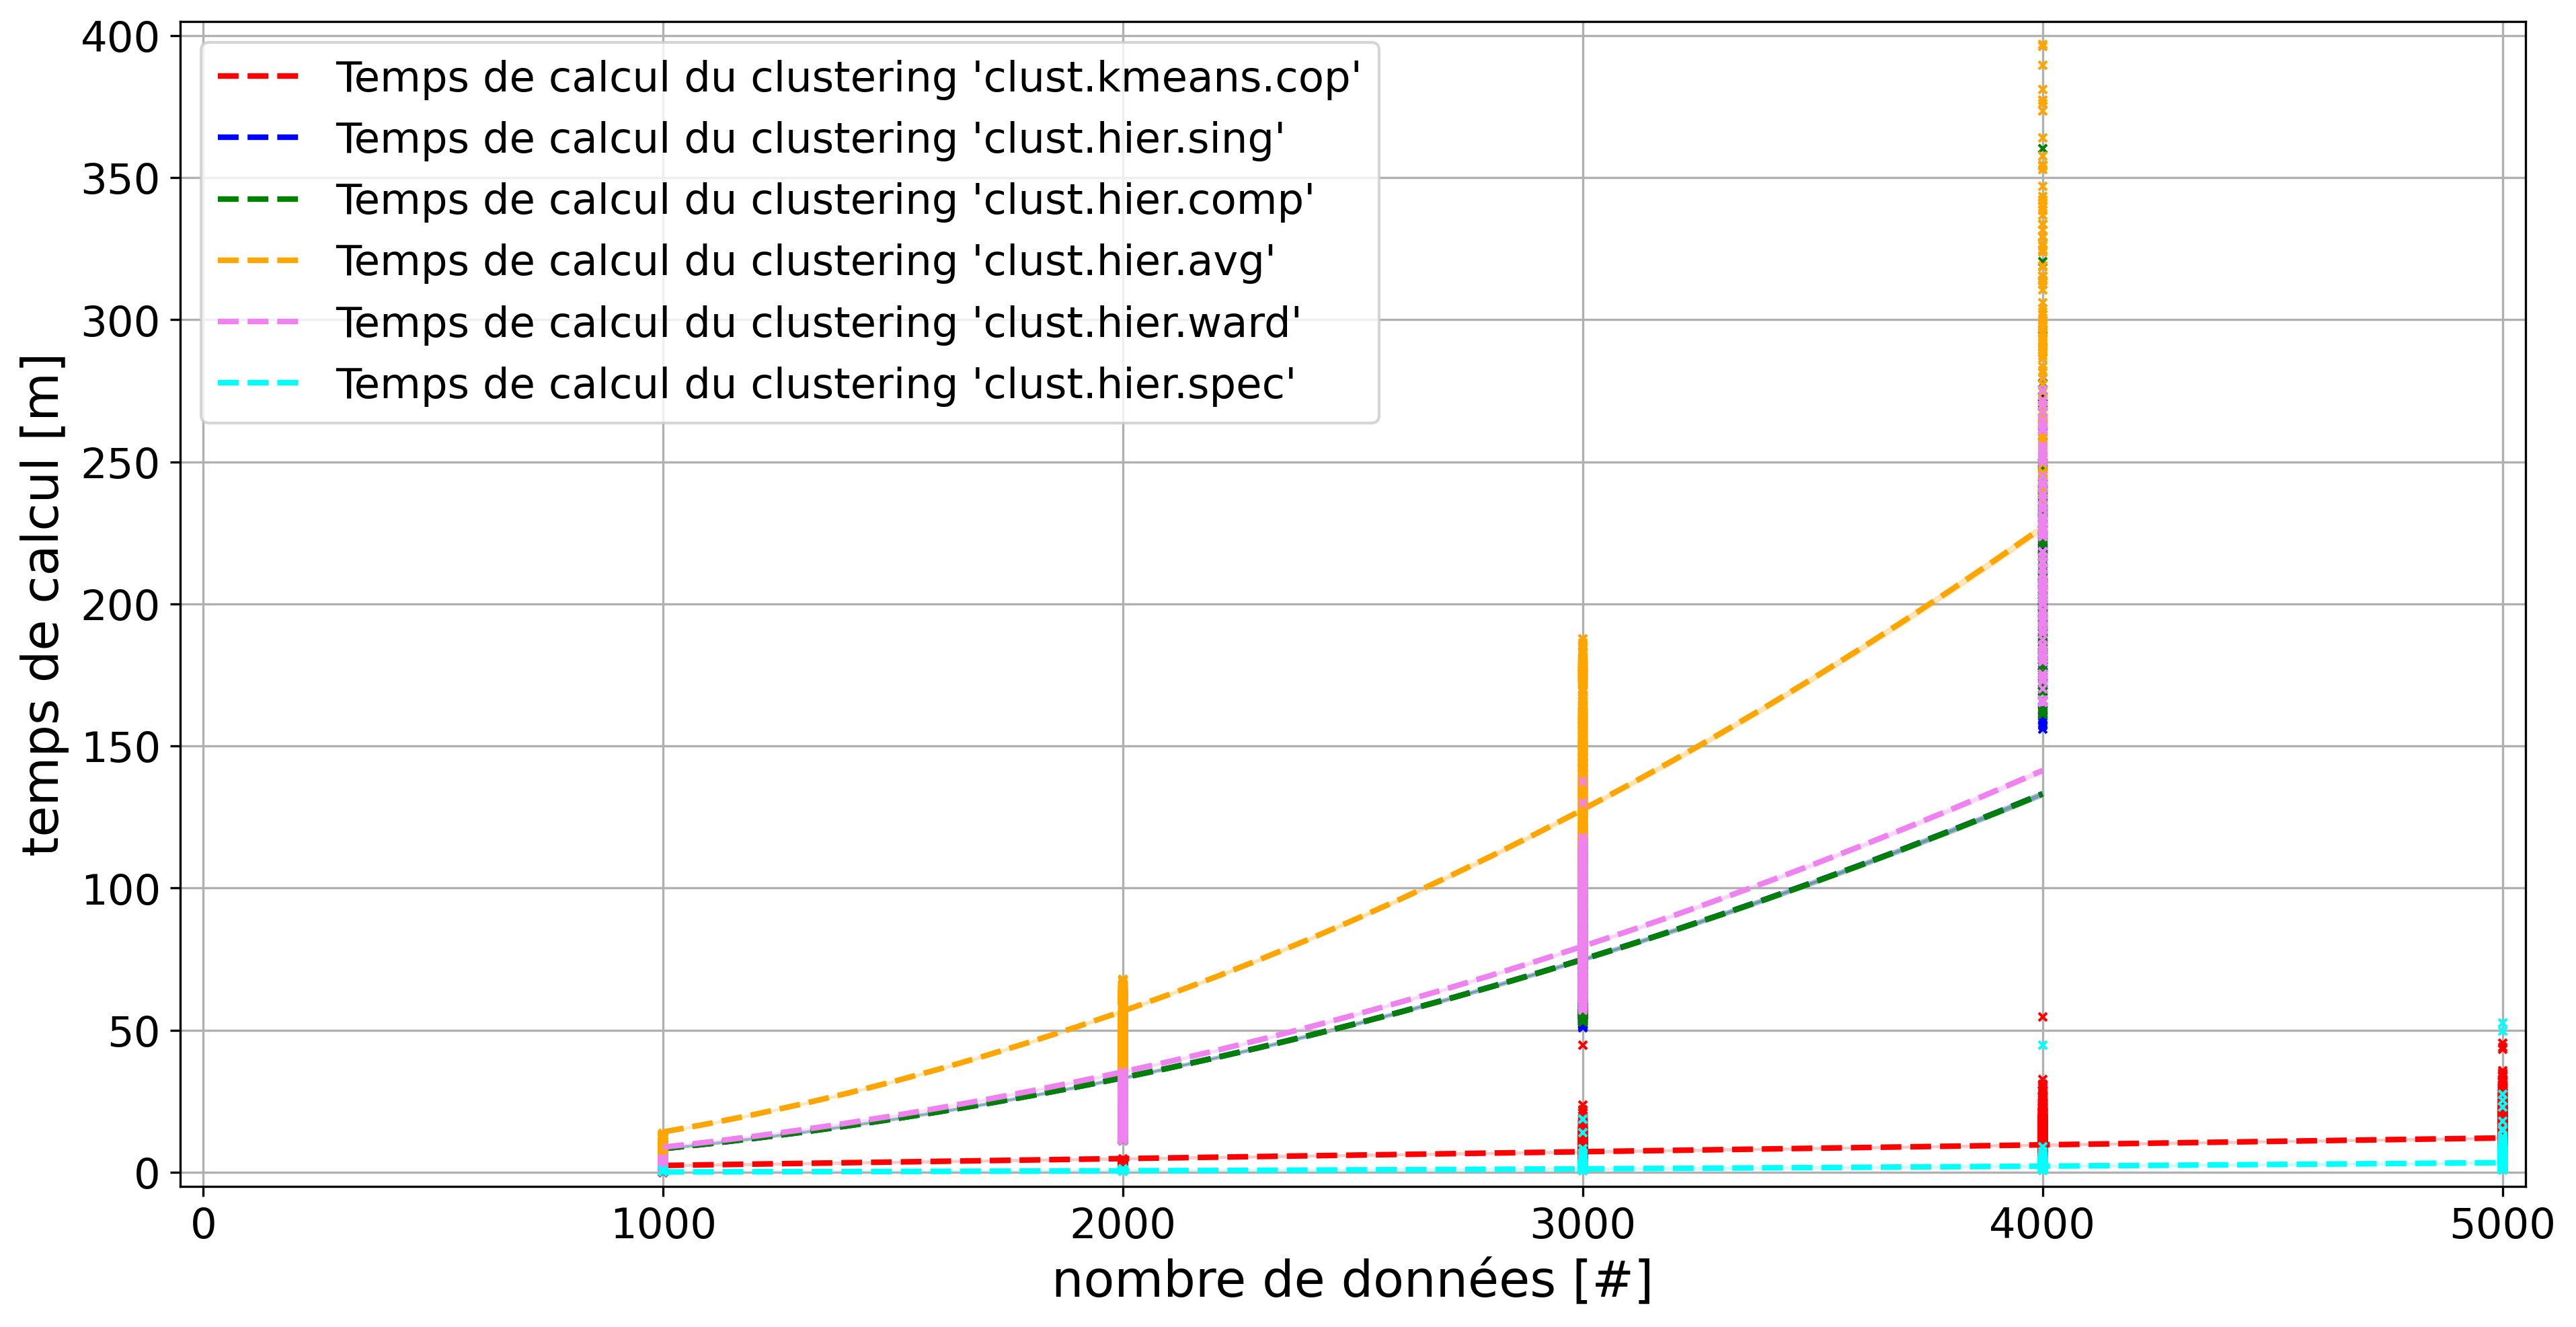
\includegraphics[width=0.95\textwidth]{figures/etude-temps-calcul-modelisation-3clust}
				\caption{
					Estimation du temps nécessaire (en minutes) pour effectuer une tâche de \textbf{clustering} en fonction du nombre de données à traiter.
				}
				\label{figure:4.3.2-ETUDE-COUTS-TEMPS-CALCUL-MODELISATION-CLUSTERING}
			\end{figure}
			
			%%% Sampling
			
			% Première analyse.
			En ce qui concerne la tâche d'\textbf{échantillonnage de contraintes}, une première analyse montre que les modélisations des quatre implémentations sont différentiables  (\texttt{p-valeur}: $<$ \texttt{$10^{-3}$}). Nous faisons donc une modélisation par algorithme.
			
			% Modélisation du temps de calcul (samp.rand.full).
			Pour les algorithmes de l'échantillonnage de contraintes \texttt{samp.rand.full}, l'analyse de la corrélation des facteurs avec les mesures de temps d'exécution indique qu'une modélisation minimale et suffisante peut être réalisée à partir du facteur $\texttt{dataset\_size}^{\textbf{2}}$ (\texttt{r}: $0.993$).
			Le second facteur le plus corrélé (mais non retenu) est l'interaction $\texttt{dataset\_size}^{\textbf{2}} \cdot \texttt{previous\_nb\_clusters}$ (\texttt{r}: $0.791$).
			Le modèle linéaire généralisé retenu (\texttt{R²}: $> 0.999$, \texttt{llf}: $-4.52 \cdot 10^{4}$, \texttt{llf\_null}: $-1.17 \cdot 10^{5}$) nous permet de déduire l'équation suivante :
			%
			\begin{equation}
				\texttt{computation\_time}(\texttt{samp.rand.full})~[s]~
				\propto~8.20 \cdot 10^{-7} \cdot \texttt{dataset\_size}^{\textbf{2}}
			\end{equation}
			
			% Modélisation du temps de calcul (samp.rand.same).
			Pour les algorithmes de l'échantillonnage de contraintes \texttt{samp.rand.same}, l'analyse de la corrélation des facteurs avec les mesures de temps d'exécution indique qu'une modélisation minimale et suffisante peut être réalisée à partir du facteur $\texttt{dataset\_size}^{\textbf{2}}$ (\texttt{r}: $0.939$).
			Le second facteur le plus corrélé (mais non retenu) est l'interaction $\texttt{dataset\_size}^{\textbf{2}} \cdot \texttt{algorithm\_nb\_constraints}$ (\texttt{r}: $0.611$).
			Le modèle linéaire généralisé retenu (\texttt{R²}: $> 0.999$, \texttt{llf}: $-3.20 \cdot 10^{4}$, \texttt{llf\_null}: $-6.84 \cdot 10^{4}$) nous permet de déduire l'équation suivante :
			%
			\begin{equation}
				\texttt{computation\_time}(\texttt{samp.rand.same})~[s]~
				\propto~1.85 \cdot 10^{-7} \cdot \texttt{dataset\_size}^{\textbf{2}}
			\end{equation}
			
			% Modélisation du temps de calcul (samp.farhtest.same).
			Pour les algorithmes de l'échantillonnage de contraintes \texttt{samp.farhtest.same}, l'analyse de la corrélation des facteurs avec les mesures de temps d'exécution indique qu'une modélisation minimale et suffisante peut être réalisée à partir du facteur $\texttt{dataset\_size}^{\textbf{2}}$ (\texttt{r}: $0.981$).
			Le second facteur le plus corrélé (mais non retenu) est l'interaction $\texttt{dataset\_size}^{\textbf{2}} \cdot \texttt{previous\_nb\_clusters}$ (\texttt{r}: $0.700$).
			Le modèle linéaire généralisé retenu (\texttt{R²}: $> 0.999$, \texttt{llf}: $-4.56 \cdot 10^{4}$, \texttt{llf\_null}: $-1.02 \cdot 10^{5}$) nous permet de déduire l'équation suivante :
			%
			\begin{equation}
				\texttt{computation\_time}(\texttt{samp.farhtest.same})~[s]~
				\propto~5.19 \cdot 10^{-7} \cdot \texttt{dataset\_size}^{\textbf{2}}
			\end{equation}
			
			% Modélisation du temps de calcul (samp.closest.diff).
			Pour les algorithmes de l'échantillonnage de contraintes \texttt{samp.closest.diff}, l'analyse de la corrélation des facteurs avec les mesures de temps d'exécution indique qu'une modélisation minimale et suffisante peut être réalisée à partir du facteur $\texttt{dataset\_size}^{\textbf{2}}$ (\texttt{r}: $0.995$).
			Le second facteur le plus corrélé (mais non retenu) est l'interaction $\texttt{dataset\_size}^{\textbf{2}} \cdot \texttt{previous\_nb\_clusters}$ (\texttt{r}: $0.815$).
			Le modèle linéaire généralisé retenu (\texttt{R²}: $> 0.999$, \texttt{llf}: $-5.96 \cdot 10^{4}$, \texttt{llf\_null}: $-1.36 \cdot 10^{5}$) nous permet de déduire l'équation suivante :
			%
			\begin{equation}
				\texttt{computation\_time}(\texttt{samp.closest.diff})~[s]~
				\propto~1.43 \cdot 10^{-6} \cdot \texttt{dataset\_size}^{\textbf{2}}
			\end{equation}
			
			% Affichage du temps de calcul.
			La \textsc{Figure~\ref{figure:4.3.2-ETUDE-COUTS-TEMPS-CALCUL-MODELISATION-SAMPLING}} représente ces modélisations de temps de calcul des algorithmes d'échantillonnage en comparaison avec les mesures réalisées lors de l'expérience.
			\newline
			%
			\begin{figure}[!htb]
				\centering
				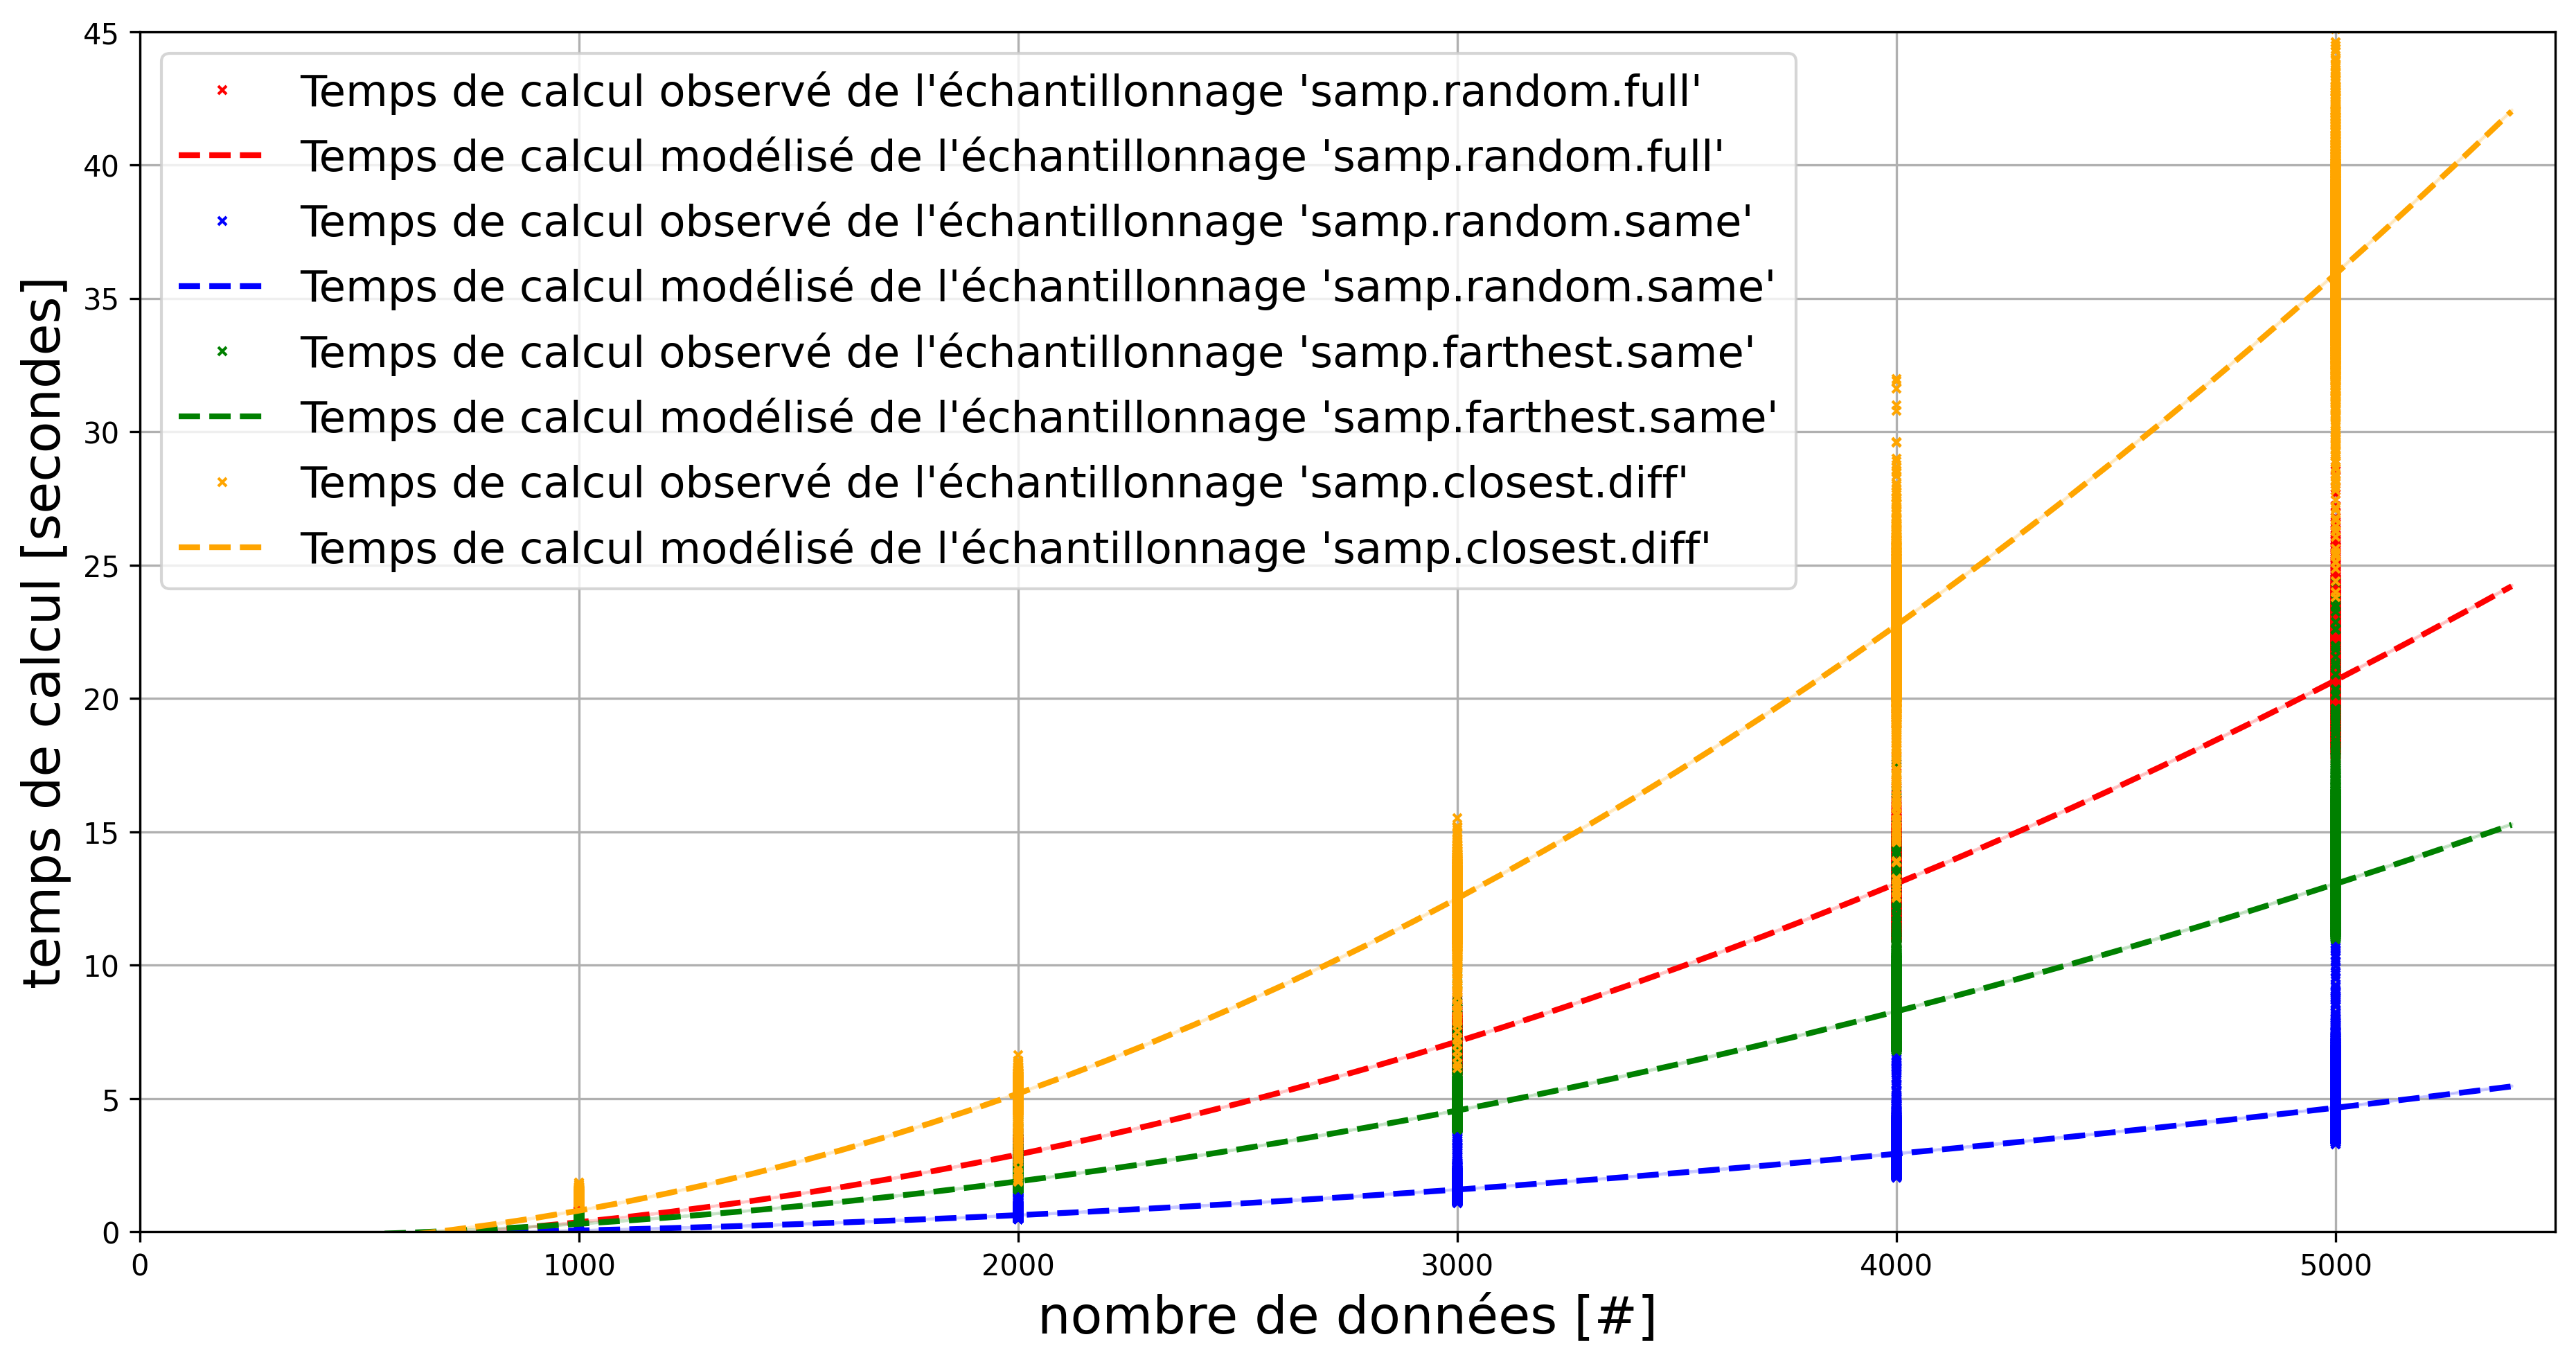
\includegraphics[width=0.95\textwidth]{figures/etude-temps-calcul-modelisation-4samp}
				\caption{
					Estimation du temps nécessaire (en minutes) pour effectuer une tâche d'\textbf{échantillonnage de contraintes} en fonction du nombre de données à traiter.
				}
				\label{figure:4.3.2-ETUDE-COUTS-TEMPS-CALCUL-MODELISATION-SAMPLING}
			\end{figure}

		%%% Discussion.
		\subsubsection{Discussion}
		
			% Rappel de l'objectif : estimer le temps d'exécution.
			Dans cette étude, nous avons estimé le temps de calcul des différents algorithmes implémentés afin de confirmer le choix de paramétrage pour une convergence optimal (cf. hypothèse d'efficience en \textsc{Section~\ref{section:4.2-HYPOTHESE-EFFICIENCE}}).
			Ces estimations ont été réalisées sur la base de plusieurs exécutions et fonction de divers contextes d'utilisation : nombre de données, nombre de contraintes annotées, nombre de contraintes à sélectionner, nombre de \textit{clusters} existant, nombre de \textit{clusters} à trouver.
			\\
			
			% Remarque générale : Dépend principalement du nombre de données.
			En premier lieu, on peut constater que les différentes modélisations dépendent majoritairement de la taille du jeu de données manipulé ($\texttt{dataset\_size}$ ou $\texttt{dataset\_size}^{\textbf{2}}$) avec un score de corrélation \texttt{r} avec le temps mesuré généralement supérieur à $0.9$ et des modèles \textit{GLM} avec des coefficients de détermination généralisé \texttt{R²} généralement proches de $0.999$.
			Bien que d'autres facteurs peuvent intervenir dans ces estimations (notamment les interactions doubles entre la taille du jeu de données et le nombre de \textit{clusters} ou le nombre de contraintes), ces derniers semblent avoir un impact négligeable sur le temps d'exécution.
			
			% Note: remarque sur le nombre de contraintes.
			\begin{leftBarAuthorOpinion}
				Certains paramétrages de la méthode du \textit{clustering} interactif semblent cependant avoir un temps de calcul décroissant au cours des itérations, mais nous n'avons cependant pas pu montrer de tendances globales significatives.
				Il est probable que l'ajout de contraintes judicieusement placées permettent à certains algorithmes de \textit{clustering} de s'exécuter plus rapidement, notamment lorsque ceux-ci exploitent les composants connexes du graphe de contraintes (cf. \textsc{Section~\ref{section:3.3.2-GESTION-DES-CONTRAINTES}}). En effet, :
				\begin{itemize}
					\item les \textit{clustering} hiérarchiques s'initialisent autant de \textit{clusters} que de groupes de données liées entre elles par des contraintes \texttt{MUST-LINK} : or s'il y a plus de contraintes, alors les composants connexes sont davantage développés, donc il y a moins de \textit{clusters} à initialiser et donc moins d'époques de l'algorithme ;
					\item le \textit{clustering} KMeans (modèle COP) attire auprès d'un barycentre l'ensemble des données liées par un \texttt{MUST-LINK} : or s'il y a plus de contraintes, alors il y a des données attirées, donc les noyaux de \textit{clusters} peuvent se stabiliser plus rapidement.  
				\end{itemize}
				Toutefois, ces suppositions n'ont pas pu être démontrées, et certains contre-exemples tendent à conclure que ces comportements sont très dépendants du jeu de données manipulé et de l'ordre d'ajout des contraintes. Par exemple :
				\begin{itemize}
					\item l'ajout d'un trop grand nombre de contraintes \texttt{CANNOT-LINK} peut engendrer un surplus de vérification pour estimer quelles formations de \textit{clusters} sont autorisées sans violer de contraintes ;
					\item l'algorithme KMeans (modèle COP) peut osciller autour de plusieurs noyaux de \textit{clusters} instables si les contraintes violent trop la similarité intrinsèque des données.
				\end{itemize}
			\end{leftBarAuthorOpinion}
			
			% Cas du clustering.
			En ce qui concerne la tâche de \textit{clustering}, on note des différences significatives dans les temps d'exécution des divers algorithmes implémentés.
			En effet, l'algorithme KMeans (modèle COP) est nettement plus rapide (complexité estimée en $ \mathcal{O}(\texttt{dataset\_size}) $, nécessitant quelques dizaines de minutes pour $5~000$ données) que les implémentations du \textit{clustering} hiérarchique (complexité estimée en $ \mathcal{O}(\texttt{dataset\_size}^{\textbf{2}}) $, nécessitant plusieurs heures dès $3~000$ données).
			Cette différence, visible en \textsc{Figure~\ref{figure:4.3.2-ETUDE-COUTS-TEMPS-CALCUL-MODELISATION-CLUSTERING}}, a un réel impact sur l'expérience utilisateur de l'opérateur.
			En effet, bien qu'il soit théoriquement plus efficient pour atteindre une annotation suffisante (cf. hypothèse d'efficience en \textsc{Section~\ref{section:4.2-HYPOTHESE-EFFICIENCE}}), l'usage d'un \textit{clustering} hiérarchique imposerait de longs temps d'attente à l'opérateur, interdisant des interactions rapides avec la machines.
			Or l'intérêt principal de notre méthodologie d'annotation à l'aide du \textit{clustering} interactif repose sur ces interactions homme-machine via l'ajout régulier de contraintes pertinentes (cf. hypothèse d'efficacité en \textsc{Section~\ref{section:4.1-HYPOTHESE-EFFICACITE}}).
			Nous décidons donc d'exclure l'usage des algorithmes de \textit{clustering} hiérarchique au profit du \textit{clustering} KMeans (modèle COP).
			
			% Note: Cas du projet étudiant avec TPS.
			\begin{leftBarInformation}
				Dans le cadre du projet étudiant avec l'école Télécom Physique Strasbourg visant à implémenter d'autres algorithmes de \textit{clustering} sous contraintes, un résonnement similaire a été utilisé pour filtrer les algorithmes. Ainsi, l'implémentation de KMeans (modèle MPC) a été exclu (complexité estimée en $ \mathcal{O}(\texttt{dataset\_size}^{\textbf{3}}) $) et l'implémentation de la propagation par affinité écarte la gestion des contraintes \texttt{CANNOT-LINK} pour avoir un temps d'exécution comparable au \textit{clustering} KMeans (modèle COP). L'algorithme DBScan (modèle C-DBScan) est quand à lui un rival possible avec une complexité estimée en $ \mathcal{O}(\texttt{dataset\_size}) $.
			\end{leftBarInformation}
			
			% Cas du prétraitement + vectorisation + échantillonnage.
			En ce qui concerne les tâches de prétraitements (cf. \textsc{Figure~\ref{figure:4.3.2-ETUDE-COUTS-TEMPS-CALCUL-MODELISATION-PREPROCESSING}}), de vectorisation (cf. \textsc{Figure~\ref{figure:4.3.2-ETUDE-COUTS-TEMPS-CALCUL-MODELISATION-VECTORIZATION}}), et d'échantillonnage de contraintes (cf. \textsc{Figure~\ref{figure:4.3.2-ETUDE-COUTS-TEMPS-CALCUL-MODELISATION-SAMPLING}}) ont des complexités presque négligeables en représentant moins de $10$\% des temps d'exécution du \textit{clustering} (pour $5~000$ données : moins de $1$ minute pour les trois algorithmes, contre $12.1$ minutes pour \texttt{clust.kmeans.cop} et $3.5$ heures pour \texttt{clust.hier.sing}).
			Nous maintenons donc les paramétrages obtenus pour ces tâches en \textsc{Section~\ref{section:4.2-HYPOTHESE-EFFICIENCE}} sans analyses complémentaires, et nous utilisons l'estimation temporelle du \textit{clustering} \texttt{clust.kmeans.cop} majorée de $10$\%.
			
			% Conclusion.
			\begin{leftBarSummary}
				Dans l'optique d'atteindre de manière efficiente $90$\% de \texttt{v-measure}\footnote{
					$90$\% de \texttt{v-measure}: cas d'une annotation dite partielle, dont le paramétrage le plus efficient est constitué du prétraitement simple (\texttt{prep.simple}), de la vectorisation TF-IDF (\texttt{vect.tfidf}), du \textit{clustering} hiérarchique à lien moyen (\texttt{clust.hier.avg}) et de l'échantillonnage des données les plus proches dans des clusters différents (\texttt{sampl.closest.diff})
				}
				avec un coût global minimal, nous retenons l'usage du \textbf{paramétrage favori} constitué du prétraitement simple (\texttt{prep.simple}), de la vectorisation TF-IDF (\texttt{vect.tfidf}), du \textit{clustering} KMeans avec modèle COP (\texttt{clust.kmeans.cop}) et de l'échantillonnage des données les plus proches dans des clusters différents (\texttt{sampl.closest.diff}).
				On estime le temps d'exécution de ce paramétrage avec l'équation suivante\footnote{
					Temps du paramétrage favori : environ $2.8$ minutes pour $1~000$ données ; environ $14.2$ minutes pour $5~000$ données.
				} :
				%
				\begin{equation}
					\label{equation:4.3.2-ETUDE-COUTS-TEMPS-CALCUL-PARAMETRAGE-FAVORI}
					\texttt{computation\_time}(\texttt{settings.favorite})~[s]~
					\propto~0.17 \cdot \texttt{dataset\_size}
				\end{equation}
			\end{leftBarSummary}
	
	%%%
	%%% Subsection 4.3.3: Étude du nombre de contraintes nécessaires à la convergence vers une vérité terrain pré-établie en fonction de la taille du jeu de données 
	%%%
	\subsection{Étude du nombre de contraintes nécessaires à la convergence vers une vérité terrain pré-établie en fonction de la taille du jeu de données}
	\label{section:4.3.3-ETUDE-COUT-NOMBRE-CONTRAINTES}
			
		% Transition.
		Avec les deux précédentes études, nous sommes capable d'estimer le temps nécessaire à un expert pour annoter des contraintes et le temps nécessaire à la machine pour proposer un nouveau \textit{clustering} adapté aux suggestions de l'expert.
		Pour poursuivre nos études et pouvoir estimer le coût total d'un projet d'annotation, il nous reste à estimer le nombre total de contraintes à devoir renseigner en fonction de la taille du jeu de données.
		
		% Objectif de l'expérience.
		Pour cela, nous allons simuler la création de cette base d'apprentissage en adaptant le protocole utilisé lors de notre étude d'efficacité (cf. \textsc{Section~\ref{section:4.1.1-ETUDE-CONVERGENCE}}) :
		nous employons notre méthode de \textit{clustering} interactif avec notre \textbf{paramétrage favori}\footnote{
			Paramétrage favori (atteindre $90$\% de \texttt{v-measure} avec un coût minimal): prétraitement simple (\texttt{prep.simple}), vectorisation TF-IDF (\texttt{vect.tfidf}), \textit{clustering} KMeans avec modèle COP (\texttt{clust.kmeans.cop}) et échantillonnage des données les plus proches dans des clusters différents (\texttt{sampl.closest.diff})
		}
		sur des jeux de données de différentes tailles et mesurons le nombre de contraintes nécessaires pour converger vers la vérité terrain.
	
		%%% Protocole expérimental.
		\subsubsection{Protocole expérimental}
			
			% Axiome.
			\begin{leftBarWarning}
				Dans le cadre de cette étude, nous supposons que l'expert métier connaît parfaitement le domaine traité dans ce jeu de données, et qu'il est capable de caractériser sans ambiguïté la similitude entre deux données issues de cet ensemble.
			\end{leftBarWarning}
			
			% Pseudo-code.
			Pour résumer le protocole expérimental que nous décrivons ci-dessous, vous pouvez vous référer au pseudo-code décrit dans \textsc{Algorithme~\ref{algorithm:4.3.3-ETUDE-COUT-NOMBRE-CONTRAINTES-PROTOCOLE}}.
			
			\begin{algorithm}
				\KwData{jeux de données annotées (vérités terrains) de tailles différentes}
				%
				\ForEach{jeux de données à tester}{
					\textbf{initialisation (données)}: récupérer ou générer les données et la vérité terrain \;
					\textbf{initialisation (contraintes)}: créer une liste vide de contraintes \;
					\textbf{prétraitement}: supprimer le bruit dans les données avec \texttt{prep.simple} \;
					\textbf{vectorisation}: transformer les données en vecteurs avec \texttt{vect.tfidf} \;
					\textbf{clustering initial}: regrouper les données par similarité avec \texttt{clust.kmeans.cop} \;
					\textbf{évaluation}: estimer l'équivalence entre le \textit{clustering} et la vérité terrain \;
					\Repeat{annotation de toutes les contraintes possibles}{
						\textbf{échantillonnage}: sélectionner des contraintes avec \texttt{samp.closest.diff} \;
						\textbf{simulation d'annotation}: déterminer les contraintes avec la vérité terrain \;
						\textbf{intégration}: ajouter les nouvelles contraintes au gestionnaire de contraintes \;
						\textbf{clustering}: regrouper les données par similarité avec \texttt{clust.kmeans.cop} \;
						\textbf{évaluation}: estimer l'équivalence entre le \textit{clustering} et la vérité terrain \;
					}
				}
				\textbf{analyse}: entraîner un modèle linéaire généralisé du nombre de contraintes nécessaires \;
				%
				\KwResult{modélisation du nombre de contraintes nécessaires pour un jeu de données}
				%
				\caption{\textit{
					Description en pseudo-code du protocole expérimental de l'étude du nombre de contraintes nécessaires pour converger vers une vérité terrain pré-établie avec notre paramétrage favori du \textit{clustering} interactif.
				}}
				\label{algorithm:4.3.3-ETUDE-COUT-NOMBRE-CONTRAINTES-PROTOCOLE}
			\end{algorithm}
			
			% Description des jeux de données.
			Nous utilisons deux vérités terrains comme références pour cette expérience :
			\begin{itemize}
				% Bank Cards.
				\item le jeu de données \texttt{Bank Cards (v2.0.0)} :
				ce dernier traite des demandes les plus fréquentes des clients en ce qui concerne la gestion de leur carte bancaire.
				Il est composé de $1~000$ questions rédigées en français et réparties en $10$ classes (\texttt{perte ou vol de carte}, \texttt{carte avalée}, \texttt{commande de carte}, ...).
				Pour plus de détails, consultez l'annexe~\ref{annex:A.1-DATASET-BANK-CARDS} ;
				% MLSUM.
				\item le jeu de données \texttt{MLSUM FR Train Subset (v1.0.0-schild)} :
				ce dernier concerne les titres d'articles de journaux issus des catégories de publication les plus communes.
				Il est composé de $744$  titres d'articles rédigés et répartis en $14$ classes (\textit{économie}, \textit{sport}, ...).
				Pour plus de détails, consultez l'annexe~\ref{annex:A.2-DATASET-MLSUM-SUBSET-SCHILD} ;
			\end{itemize}

			Cependant, deux jeux de données ne nous permettent pas d'analyser l'impact du nombre de données sur le nombre de contraintes nécessaires pour converger vers une vérité terrain.
			Pour utiliser facilement plusieurs jeux de données de tailles différentes tout en maîtrisant leur contenu, nous avons donc dupliqué aléatoirement des données issues de ces jeux de référence en y insérant des fautes de frappes.
			La taille des jeux de données générés, notée $\texttt{dataset\_size}$, varie entre $1~000$ à $5~000$ par pas de $250$, et chaque taille de jeu est générée $3$ fois pour contrer les aléas statistiques de création.
			Il y a donc $51$ variations de chaque jeu de références, soit $102$ jeux utilisés de tailles différentes.
			
			% Remarque.
			\begin{leftBarWarning}
				Dans le cadre de cette étude, nous faisons l'hypothèse que cette création artificielle de données n'a pas d'impact majeur sur le nombre de contraintes nécessaires pour converger vers une vérité terrain.
			\end{leftBarWarning}
			
			% Description des tentatives de la méthode.
			Sur chacun de ces jeux générés, une tentative complète\footnote{
				Tentative complète : itérations d'échantillonnage, d'annotation et de \textit{clustering} jusqu'à annotation de toutes les contraintes possibles.
			}
			de la méthode du \textit{clustering} interactif en utilisant notre paramétrage favori est exécuté, et chaque tentative est répétée $5$ fois pour contrer les aléas statistiques des exécutions.
			Il y a donc $510$ tentatives de \textit{clustering} interactif réalisées.
			
			% Description de l'évaluation.
			Pour chacune de ces tentatives, nous nous intéressons au nombre de contraintes nécessaires pour atteindre le seuil d'annotation partielle (caractérisé par $90$\% de \texttt{v-measure} entre la vérité terrain et la segmentation des données obtenue), et nous entraînons un modèle linéaire généralisé (\textit{GLM}) pour modéliser le nombre de contraintes requis en fonction de la taille du jeu de données (noté $\texttt{dataset\_size}$).
			Ce modèle sera caractérisé par le coefficient de détermination généralisé \texttt{R²} de \textit{Cox et Snel} (\cite{diamond-etal:1990:analysis-binary-data}), la log-vraisemblance \texttt{llf} (\cite{edwards:1992:likelihood}) et la log-vraisemblance \texttt{llf\_null} du modèle \textit{null}.
			Pour finir, nous discutons des valeurs des coefficients obtenus sur l'impact du nombre d'itérations de la méthode à prévoir.

			% Référence scripts.
			\begin{leftBarInformation}
				Les scripts de l'expérience, réalisés avec des \textit{notebooks} Python (\cite{van-rossum-drake:2009:python-reference-manual}), sont disponibles dans un dossier dédié de~\cite{schild:2021:cognitivefactory-interactiveclusteringcomparativestudy}.
				Nous utilisons entre autres la librairie \texttt{statsmodels} (\cite{seabold-perktold:2010:statsmodels-econometric-statistical}).
			\end{leftBarInformation}

		%%% Résultats.
		\subsubsection{Résultats obtenus}
		
			% Modélisation du nombre de contraintes.
			Le modèle linéaire généralisé entraîné sur les mesures du nombre de contraintes requis pour atteindre $90$\% de \texttt{v-measure} (\texttt{R²}: $> 0.999$, \texttt{llf}: $-4~327.6$, \texttt{llf\_null}: $-4~942.9$) nous permet de déduire l'équation suivante :
			%
			\begin{equation}
				\label{equation:4.3.3-ETUDE-COUT-NOMBRE-CONTRAINTES}
				\texttt{constraints\_needed}(\texttt{settings.favorite})~[\#]~
				\propto~3.15 \cdot \texttt{dataset\_size}
			\end{equation}
			%
			La \textsc{Figure~\ref{figure:4.3.3-ETUDE-COUT-NOMBRE-CONTRAINTES}} représente cette modélisation.
			\newline
			%
			\begin{figure}[!htb]
				\centering
				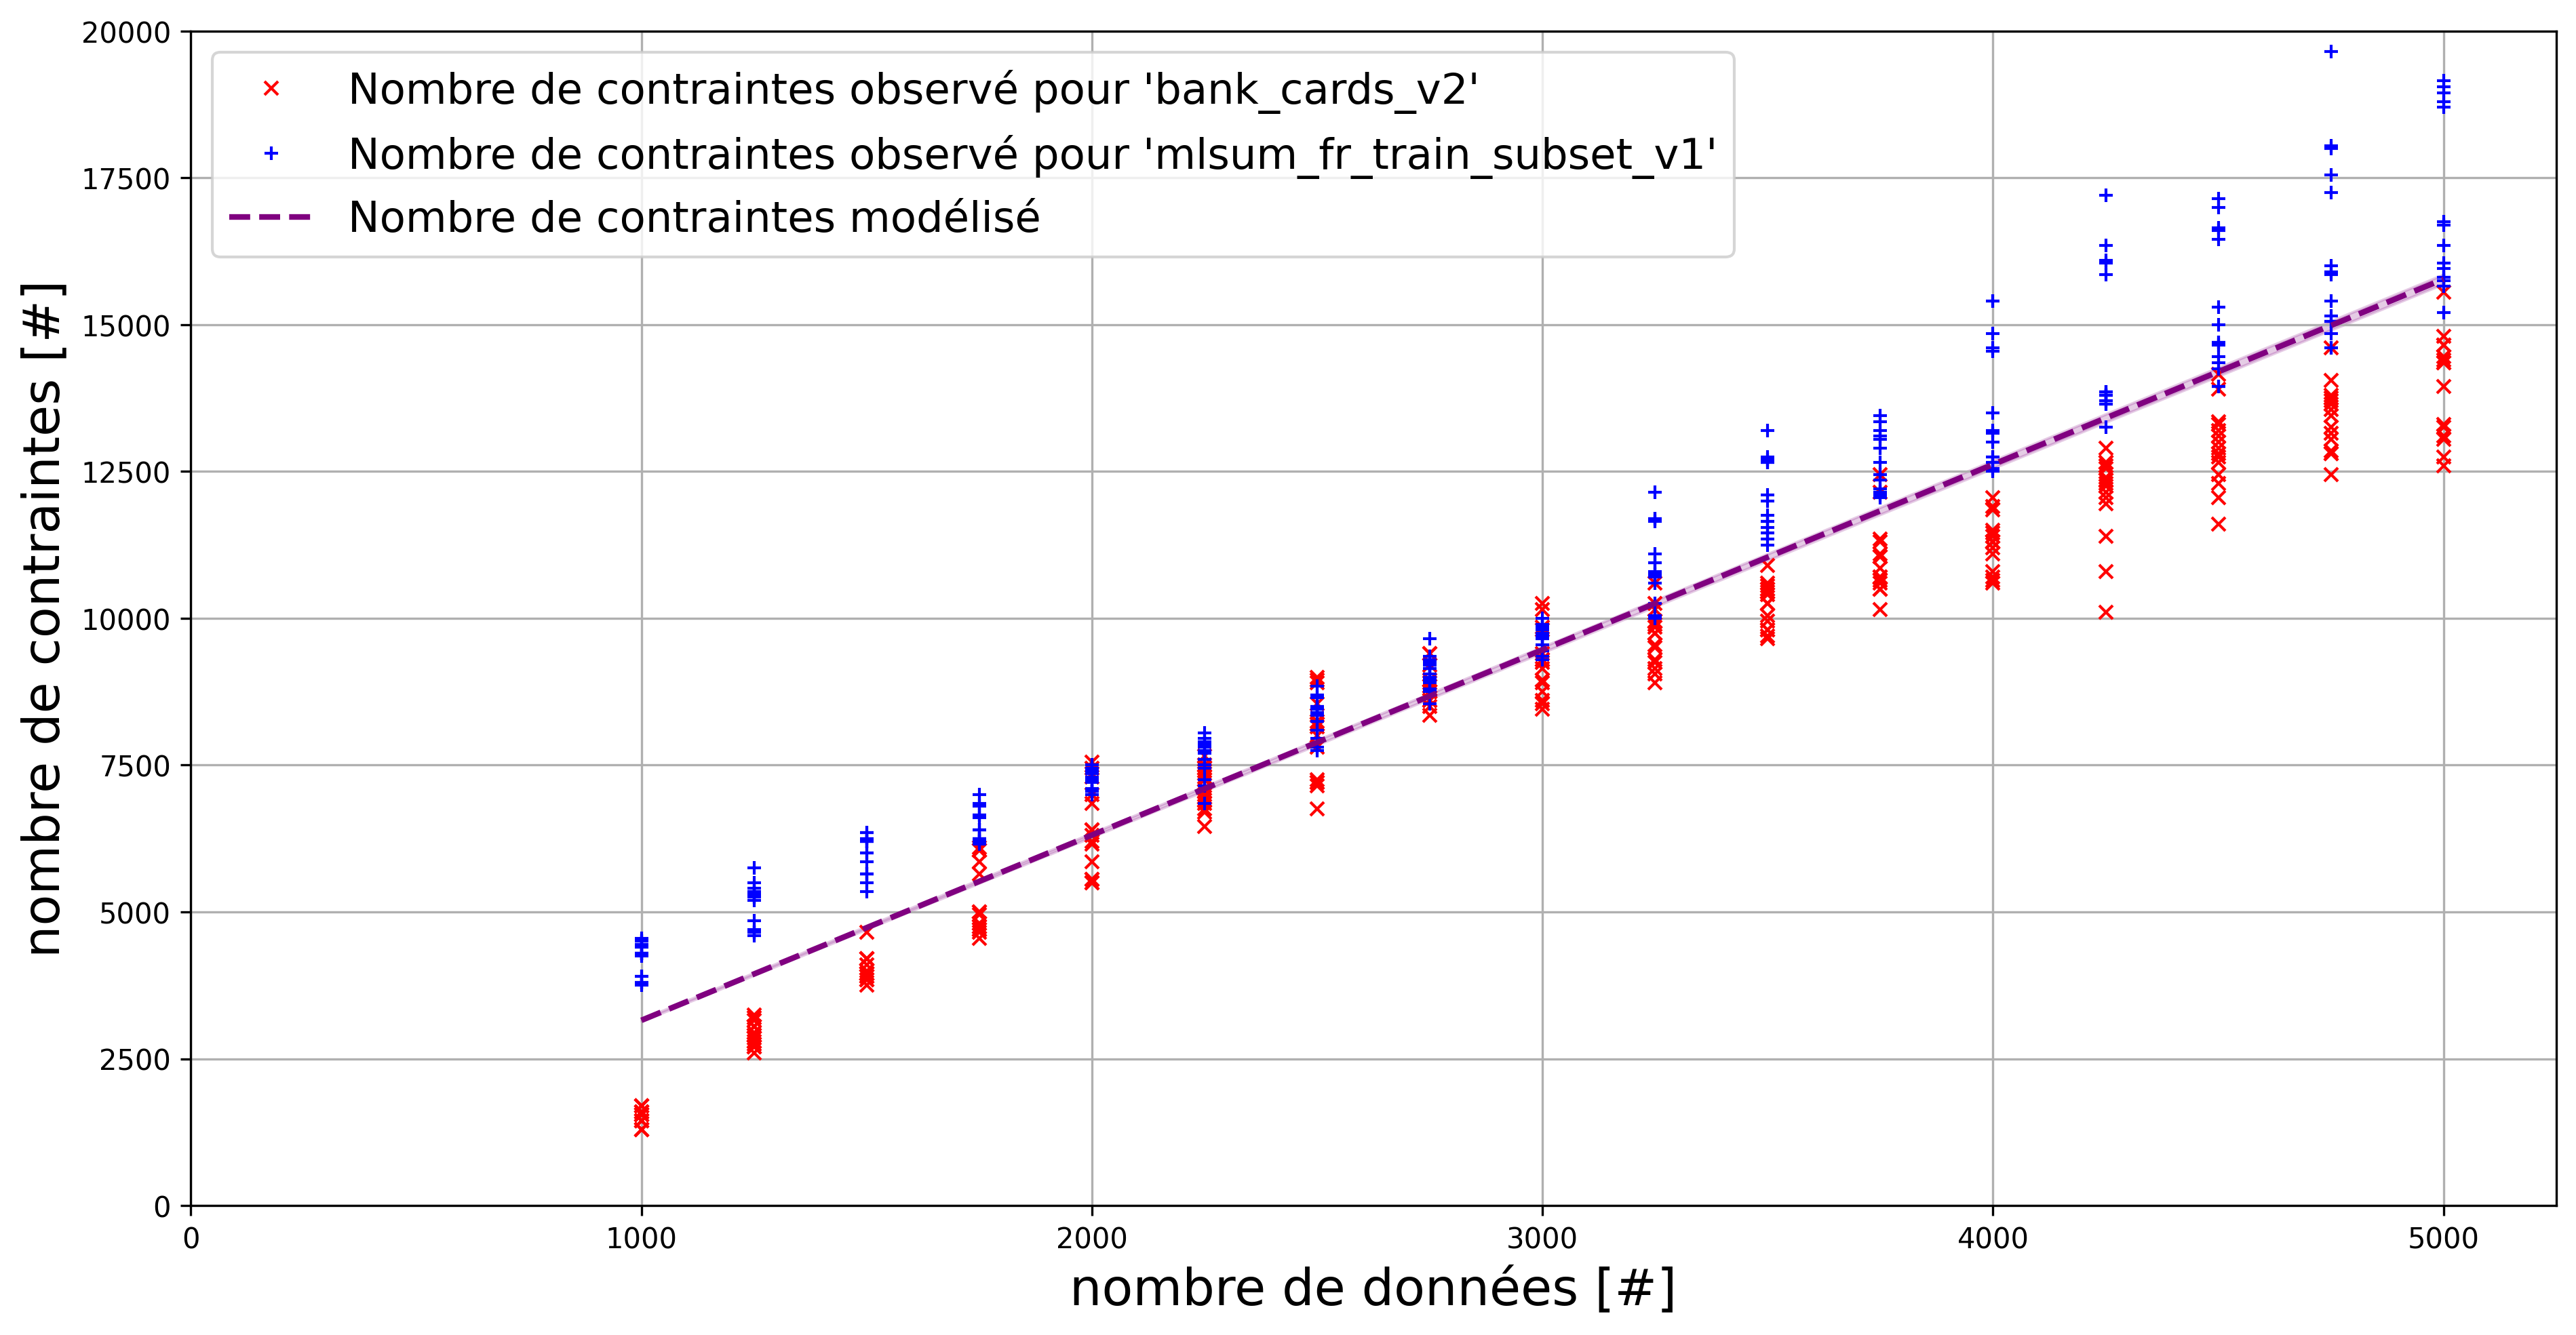
\includegraphics[width=0.95\textwidth]{figures/etude-nombre-contraintes-1-modelisation-nombre}
				\caption{
					Estimation du nombre moyen de contraintes nécessaire à notre \textbf{paramétrage favori} du \textit{clustering} interactif afin d'obtenir une annotation partielle (\textit{atteindre une \texttt{v-measure} de $90$\%}) en fonction de la taille du jeu de données à modéliser.
				}
				\label{figure:4.3.3-ETUDE-COUT-NOMBRE-CONTRAINTES}
			\end{figure}
		
			% Note de l'auteur.
			\begin{leftBarAuthorOpinion}
				% Estimation de points de références.
				On peut considérer les points de références suivants :
				\begin{itemize}
					\item le nombre de contraintes possibles (avec doublons) est de $\texttt{dataset\_size}^{\textbf{2}}$ (\textit{caractériser chaque couple de données présent dans la matrice d'adjacence}) ;
					\item le nombre de contraintes possibles (sans doublons) est de $\frac{1}{2} \cdot (\texttt{dataset\_size}^{\textbf{2}} - \texttt{dataset\_size})$ (\textit{considérer la symétrie des contraintes, donc seul le triangle supérieur de la matrice d'adjacence a besoin d'être renseigné}) ;
					\item le nombre minimal de contraintes à annoter pour être exhaustif sur une partition en $k$ \textit{clusters} $\{K_{1}, K_{2}, ..., K_{k}\} $ est estimé à ${\displaystyle \sum\limits_{1 \leq i \leq k}{(\|K_{i}\|-1)} + \sum\limits_{1 \leq i \leq k}{(k-i)}} $
					(\textit{il faut d'abord considérer les chemins minimaux pour parcourir les composants connexes avec des contraintes \texttt{MUST-LINK}, correspondant à $\|K_{i}\|-1$ contraintes \texttt{MUST-LINK} pour chaque partition $\|K_{i}\|$, puis ajouter le nombre minimal des contraintes \texttt{CANNOT-LINK} pour distinguer chacun de ses composants connexes en \textit{cluster}}, correspondant au nombre de arrangements sans répétition de deux partitions).
				\end{itemize}
				%
				% Annonce de la figure.
				La \textsc{Figure~\ref{figure:4.3.3-ETUDE-COUT-NOMBRE-CONTRAINTES-EXEMPLES}} illustre ces propos sur un jeu d'exemple comportant $10$ points de données réparties en $3$ classes, et met en avant l'explosion du nombre de contraintes possibles même sur un petit jeu de données (cf.~\ref{figure:4.3.3-ETUDE-COUT-NOMBRE-CONTRAINTES-EXEMPLES}~\textbf{(2)}).
				
				% Application de ces points de référence.
				Avec ces références, le nombre de contraintes est borné approximativement
				entre $1~035$ et $499~500$ pour un jeu de $1~000$ données équilibré en $10$ classes,
				et entre $6~175$ et $12~497~500$ pour un jeu de $5~000$ données équilibré en $50$ classes.
				%
				\begin{figure}[H]
					\centering
					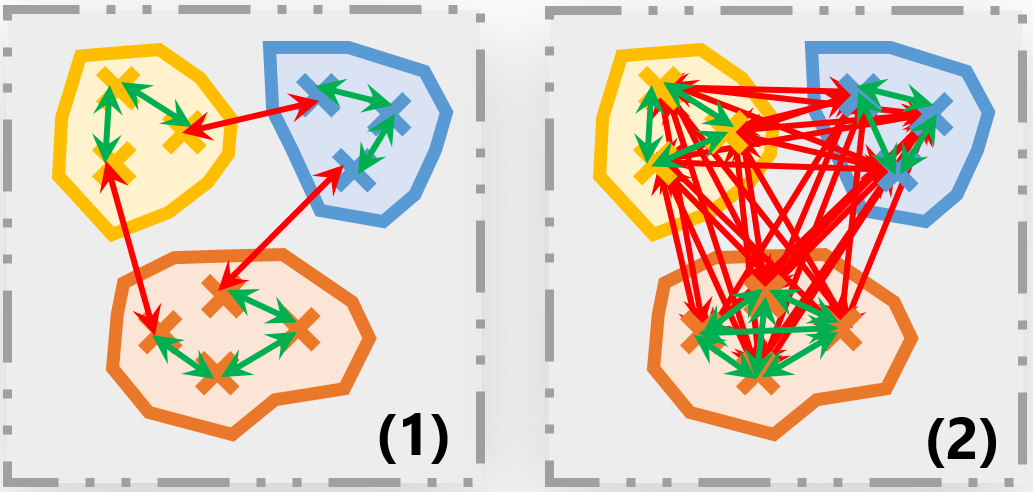
\includegraphics[width=0.5\textwidth]{figures/etude-nombre-contraintes-2-bornes-limites}
					\caption{
						Exemple de caractérisation exhaustive d'un jeu de données ($10$ données, $3$ classes) en ajoutant un nombre minimal de contraintes (cf. \textbf{(1)}) ou en ajoutant toutes les contraintes possibles (cf. \textbf{(2)}).
					}
					\label{figure:4.3.3-ETUDE-COUT-NOMBRE-CONTRAINTES-EXEMPLES}
				\end{figure}
			\end{leftBarAuthorOpinion}

		%%% Discussion.
		\subsubsection{Discussion}
		
			% Rappel de l'objectif.
			L'objectif de cette étude était de déterminer le nombre moyen de contraintes à devoir annoter pour modéliser un jeu de données avec un accord $90$\% de \texttt{v-measure} avec la vérité terrain utilisée.
			Cette estimation, dépendant de la taille du jeu de données manipulé, est représentée par l'\textsc{Equation~\ref{equation:4.3.3-ETUDE-COUT-NOMBRE-CONTRAINTES}}.
			\\
			
			% Discussion générale sur la pente.
			On peut constater que la relation entre la taille du jeu de données et le nombre de contraintes à annoter est linéaire (pente de $3.15$) : doubler la taille d'un jeu de données doublera donc la charge de travail incombant à l'expert métier.
			À première vue, une telle estimation représente une lourde charge d'annotation : \textbf{pour un jeu de $5~000$ données, il faut caractériser $15~750$ contraintes, ce qui correspond environ à $34$ heures d'annotation} d'après l'\textsc{Equation~\ref{equation:4.3.1-ETUDE-COUT-COUTS-TEMPS-ANNOTATION}} !
			Néanmoins, comme le nombre de contraintes possibles évolue en $ \mathcal{O}(\texttt{dataset\_size}) $, cette estimation aurait pu être bien pire et représenter $12~497~500$ contraintes (cf. \textsc{Figure~\ref{figure:4.3.3-ETUDE-COUT-NOMBRE-CONTRAINTES-EXEMPLES}} dans notre précédente précédente).
			Mieux encore, le nombre théorique minimal moyen de contraintes à annoter pour $5~000$ données n'est que $2.55$ fois plus faible que notre estimation ($6~175$ vs $15~750$, cf. notre précédente précédente), alors que cette borne minimale nécessite un échantillonnage "\textit{parfait}" permettant d'identifier le chemin minimal parcourant les clusters.
			Nous pouvons donc relativiser l'estimation faite avec l'\textsc{Equation~\ref{equation:4.3.3-ETUDE-COUT-NOMBRE-CONTRAINTES}} et en conclure que notre méthode un nombre de contraintes raisonnable à annoter.
			
			% Influence du jeu de données.
			Bien évidemment, une telle estimation est sensible au jeu de données utilisé comme référence (cf. \textsc{Figure~\ref{figure:4.3.3-ETUDE-COUT-NOMBRE-CONTRAINTES}}).
			Ici, la différence de pente mesurée est de $0.25$ (\texttt{p-valeur}: $> 0.999$), soit un écart moyen d'environ $8$\% par rapport à la modélisation moyenne.
			Toutefois, comme l'impact semble limité, nous maintenons la modélisation moyenne représentée par l'\textsc{Equation~\ref{equation:4.3.3-ETUDE-COUT-NOMBRE-CONTRAINTES}} pour la suite de nos estimations de coûts.
		
			% Note de l'auteur.
			\begin{leftBarAuthorOpinion}
				Il n'y a pas davantage de matière à discussion pour cette étude, car le principal résultat (l'\textsc{Equation~\ref{equation:4.3.3-ETUDE-COUT-NOMBRE-CONTRAINTES}}) est un résultat temporaire nécessaire à l'estimation du coût global d'un projet utilisant une méthodologie de \textit{clustering} interactif.
			\end{leftBarAuthorOpinion}
	
	%%%
	%%% Subsection 4.3.4: Estimation du temps total d'un projet d'annotation en combinant les précédentes études de coûts
	%%%
	\subsection{Estimation du temps total d'un projet d'annotation en combinant les précédentes études de coûts}
	\label{section:4.3.4-ETUDE-COUTS-TOTAL}
	
		% Equation finale.
		Résumons l'ensemble des modélisations réalisées lors des précédentes études (cf. sections \ref{section:4.3.1-ETUDE-COUTS-TEMPS-ANNOTATION}, \ref{section:4.3.2-ETUDE-COUTS-TEMPS-CALCUL} et \ref{section:4.3.3-ETUDE-COUT-NOMBRE-CONTRAINTES}) afin d'estimer le coût total d'un projet d'annotation employant une méthodologie basée sur le \textit{clustering} interactif et utilisant notre \textbf{paramétrage favori}\footnote{
			Paramétrage favori (atteindre $90$\% de \texttt{v-measure} avec un coût minimal).
		}.
		Dans les notations, $\texttt{dataset\_size}$ représente la taille du jeu de données à modéliser, et $\texttt{batch\_size}$ représente le nombre de contraintes que l'expert annote à chaque itération.

		%%% Résultats.
		\subsubsection{Synthèse des résultats}
			
			% Equation: Temps pour une itération (séquentielle).
			Tout d'abord, nous pouvons estimer le \textbf{temps moyen d'une itération de la méthode}, comprenant d'une part les temps d'exécution des algorithmes (\textit{prétraitement}, \textit{vectorisation}, \textit{clustering}, \textit{échantillonnage}) et d'autre part le temps d'annotation d'un lot de contraintes, grâce aux équations suivantes :
			\begin{equation}
				\label{equation:4.3.4-ETUDE-COUT-UNE-ITERATION-SEQUENTIELLE}
				\begin{cases}
					% Computation time.
					\texttt{computation\_time}~[s]&
						~\propto~0.17 \cdot \texttt{dataset\_size}\\
					% Annotation time.
					\texttt{annotation\_time}~[s]&
						~\propto~7.8 \cdot \texttt{batch\_size} \\
					% One iteration time (sequential).
					\texttt{iteration\_time(sequential)}~[s]&
						~\propto~\texttt{computation\_time} + \texttt{annotation\_time} \\
				\end{cases}
			\end{equation}
			
			% Equation: Nombre d'itérations (séquentielle).
			Ensuite, nous sommes en mesure d'anticiper le \textbf{nombre moyen de contraintes à annoter} pour modéliser le jeu de données avec un seuil de $90$\% de \texttt{v-measure}, et donc de déduire le nombre d'itérations nécessaire de la méthode, grâce aux équations suivantes :
			\begin{equation}
				\label{equation:4.3.4-ETUDE-COUT-NOMBRE-ITERATIONS-SEQUENTIEL}
				\begin{cases}
					% Constraints number.
					\texttt{constraints\_needed}~[\#] &
						~\propto~3.15 \cdot \texttt{dataset\_size} \\
					% Iterations number.
					\texttt{iterations\_needed}~[\#] &
						~\propto~\frac{\texttt{nb\_constraints}}{\texttt{batch\_size}} \\
				\end{cases}
			\end{equation}
			
			% Equation: Temps total pour un projet (séquentielle).
			Enfin, il suffit de combiner \textsc{Equation~\ref{equation:4.3.4-ETUDE-COUT-UNE-ITERATION-SEQUENTIELLE}} et \textsc{Equation~\ref{equation:4.3.4-ETUDE-COUT-NOMBRE-ITERATIONS-SEQUENTIEL}} pour estimer le temps total nécessaire à un projet d'annotation utilisant le \textit{clustering} interactif (c'est-à-dire en enchaînant successivement des étapes d'échantillonnage, d'annotation et de \textit{clustering}, cf. \textsc{Figure~\ref{figure:4.3.4-ETUDE-COUT-TOTAL-ARCHITECTURE}} (1)) pour converger vers $90$\% de \texttt{v-measure} :
			\begin{equation}
				\label{equation:4.3.4-ETUDE-COUT-TOTAL-SEQUENTIEL}
				\begin{cases}
					% Total time (sequential).
					\texttt{total\_time(sequential)}~[s] &
						~\propto~\texttt{iteration\_time} \cdot \texttt{iterations\_needed}
				\end{cases}
			\end{equation}
			
			% Figure.
			Ces estimations globales sont représentées sur la \textsc{Figure~\ref{figure:4.3.4-ETUDE-COUT-TOTAL}} en fonction de plusieurs taille de jeu de données et plusieurs tailles de lots d'annotation.

		%%% Discussion finale.
		\subsubsection{Discussion du coût total}
		
			% Rappel des objectifs.
			L'objectif de cette section consistait à déterminer les coûts relatifs à la tâche d'annotation de contraintes par un expert métier et au temps d'exécution des algorithmes intervenant dans notre implémentation du \textit{clustering} interactif.
			Pour cela, nous avons chronométré des annotateurs en situation réelle (cf. \textsc{Section~\ref{section:4.3.1-ETUDE-COUTS-TEMPS-ANNOTATION}}), estimé le temps de calcul de chaque algorithme implémenté (cf. \textsc{Section~\ref{section:4.3.2-ETUDE-COUTS-TEMPS-CALCUL}}) et trouvé le moyen de prédire le nombre de contraintes à annoter sur un jeu de données (cf. \textsc{Section~\ref{section:4.3.3-ETUDE-COUT-NOMBRE-CONTRAINTES}}).
			Nous avons pu montré qu'une annotation de contraintes est plus rapide qu'une annotation par label et nous conseillons, d'après notre analyse empirique, des sessions d'annotation de moins de $150$ contraintes pour ne pas épuiser l'annotateur.
			Sur le paramétrage de la méthode, nous avons rejeté l'usage d'algorithmes de \textit{clustering} de type hiérarchiques à cause de leur lenteur, au profit du KMeans (\texttt{clust.kmeans.cop}).
			Notre paramétrage favori, permettant d'atteindre $90$\% de \texttt{v-measure} avec un coût minimal, est ainsi constitué d'un prétraitement simple (\texttt{prep.simple}), d'une vectorisation TF-IDF (\texttt{vect.tfidf}), d'un \textit{clustering} KMeans avec modèle COP (\texttt{clust.kmeans.cop}) et d'un échantillonnage des données les plus proches dans des clusters différents (\texttt{sampl.closest.diff}).
			Enfin, pour atteindre cet objectif de \texttt{v-measure}, le nombre moyen de contraintes à annoter avec notre méthodologie semble rester linéairement proportionnel à la taille du jeu de données à modéliser, ce qui est encourageant au regard de la combinatoire de contraintes possibles.
			\\
			
			% Annonce des résultats : c'est long !
			La mise en commun de ces résultats se retrouvent dans \textsc{Equation~\ref{equation:4.3.4-ETUDE-COUT-UNE-ITERATION-SEQUENTIELLE}}, \textsc{Equation~\ref{equation:4.3.4-ETUDE-COUT-NOMBRE-ITERATIONS-SEQUENTIEL}} et \textsc{Equation~\ref{equation:4.3.4-ETUDE-COUT-TOTAL-SEQUENTIEL}}.
			Comme le nombre de données à annoter est inversement proportionnel au nombre d'itération à réaliser, nous avons le dilemme suivant : soit nous annotons de petits lots ($50$ contraintes) pour rapidement intégrer les contraintes et permettre à l'annotateur de se reposer régulièrement, mais ce dernier va en contrepartie devoir attendre plus souvent la fin des exécutions du \textit{clustering} ; soit nous annotons des lots plus conséquents ($150$ contraintes) pour diminuer le nombre d'itérations et exécuter moins de \textit{clustering}, mais cela risque d'épuiser l'opérateur avec des grosses charges d'annotation.
			Dans les deux cas, \textbf{le coût total semble élevé} : pour un jeu de $5~000$ points de données, et avec des tailles d'échantillons compris entre $50$ et $150$ contraintes, il faut entre $59$ et $110$ heures de travail (\textit{$34$ heures d'annotations et entre $25$ et $76$ heures d'attente de la fin d'exécution d'algorithmes suivant la taille des lots}).
			En considérant une journée de travail de $7$ heures, cela représente une charge contenue entre $8.4$ et $15.7$ jours pour avoir un jeu de donnée fiable à $90$\% de \texttt{v-measure}.
			Pour finir, nous ajoutons $1$ jour pour combler l'écart théorique de $10$\% de \texttt{v-measure} en corrigeant manuellement le résultat obtenu, et $1$ jour supplémentaire pour interpréter et nommer chaque \textit{cluster} (voir. \textsc{Algorithme~\ref{algorithm:3.2-CLUSTERING-INTERACTIF}}, \textit{ligne 13}).
			Au final, pour un ensemble de $5~000$ données, il faut donc entre $8.4$ {\footnotesize $(+2)$} et $15.7$ {\footnotesize $(+2)$} jours de travail à un expert métier pour obtenir une base d'apprentissage avec une méthodologie basée sur le \textit{clustering} interactif.
			
			% Critique du résultat : comparaison avec une annotation classique, avoir plusieurs annotateurs, ...
			Pour critiquer l'approximation que nous avons faite lors de cette section, nous essayons de la comparer le temps nécessaire qu'il aurait fallu à un projet d'annotation traditionnelle, comme décrit en \textsc{Section~\ref{section:2.2.1-ORGANISATION-ANNOTATION-ETAPES-CLES}} (cycle \texttt{MATTER}), et notre proposition de cycle d'annotation avec le \textit{clustering} interactif, visible en \textsc{Figure~\ref{figure:4.3.4-ETUDE-COUT-TOTAL-ARCHITECTURE}} (1).
			En nous basant sur un ensemble de $5~000$ données à annoter, nous estimons qu'il faut :
			$1$ jour de travail pour définir une représentation des données en modèle de classification ;
			$4$ jours de travail pour annoter $5~000$ données (à raison de $20$ secondes par données, estimation haute inspirée de \cite{pradhan-etal:2007:semeval2007-task-17} où la "\textit{désambiguïsation du sens des mots}", présentée comme une tâche de classification, demande $17.5$ secondes par données) ;
			$2$ jours de marge d'erreur pour changer de modèle de représentation s'il ne semble pas adapté aux données en cours d'annotation.
			Au total, nous estimons donc qu'il faut $5$ {\footnotesize $(+2)$} jours de travail à un expert métier pour obtenir une base d'apprentissage avec une méthodologie traditionnelle.
			\textbf{En l'état, nous pouvons donc conclure que le \textit{clustering} interactif que nous proposons est en moyenne deux fois plus coûteux qu'une annotation manuelle classique ($8.4$ {\footnotesize $(+2)$} à $15.7$ {\footnotesize $(+2)$} jours vs $5$ {\footnotesize $(+2)$} jours), ce qui peut être un frein à son utilisation en situation réelle}.
			
			% Pistes d'amélioration : Augmenter la taille des lots d'annotation + Augmenter le nombre d'annotateurs + paralléliser annotation et clustering, ...
			Afin d'accélérer la phase d'annotation et de diminuer le nombre d'itérations, il est bien entendu possible d'augmenter la taille des échantillons de contraintes à annoter ou d'ajouter plusieurs opérateurs.
			Cependant, une telle solution ne permet toujours pas d'être compétitif avec l'annotation traditionnelle si cette dernière dispose aussi de plusieurs opérateurs (\textit{avec $2$ annotateurs : de $6.5$ {\footnotesize $(+2)$} à $13.3$ {\footnotesize $(+2)$} jours vs $3$ {\footnotesize $(+2)$} jours ; avec $4$ annotateurs : de $4.8$ {\footnotesize $(+2)$} à $12.1$ {\footnotesize $(+2)$} jours vs $2$ {\footnotesize $(+2)$} jours}).
			Une autre piste, plus prometteuse, consiste plutôt à adapter notre méthode pour exploiter les temps d'attente lors de l'exécution d'un \textit{clustering}.
			

		%%% Ouverture
		\subsection{Ouverture vers une annotation en parallèle du \textit{clustering}}
		
			% Idée : Optimiser le temps d'attente.
			Notre méthodologie d'annotation basée sur le \textit{clustering} interactif est pénalisée par la séquentialité des actions à réaliser.
			En effet, l'annotateur doit attendre la fin d'un de l'exécution des algorithmes de \textit{clustering} et d'échantillonnage avant de pouvoir travailler.
			D'après nos précédentes estimations sur un jeu de $5~000$ données, l'opérateur doit attendre entre $25$ et $76$ heures en fonction de la taille de lots d'annotation choisie, et une idée à explorer consiste à optimiser ce temps d'attente.
			
			% Réalisation : Paralléliser annotation et \textit{clustering} !
			L'amélioration envisagée consiste à \textbf{réaliser l'annotation de contraintes en parallèle de l'exécution du \textit{clustering}}, comme représenté dans la \textsc{Figure~\ref{figure:4.3.4-ETUDE-COUT-TOTAL-ARCHITECTURE}} (2).
			Dans cette version, l'échantillonnage se base toujours sur le résultat du \textit{clustering} de l'itération précédente, mais le \textit{clustering} intègre les contraintes annotées avec un décalage d'une itération.
			Un tel changement permet de limiter le temps d'attente de l'opérateur et d'optimiser l'enchaînement des algorithmes.

			% Figure architecture.
			\begin{figure}[!htb]
				\centering
				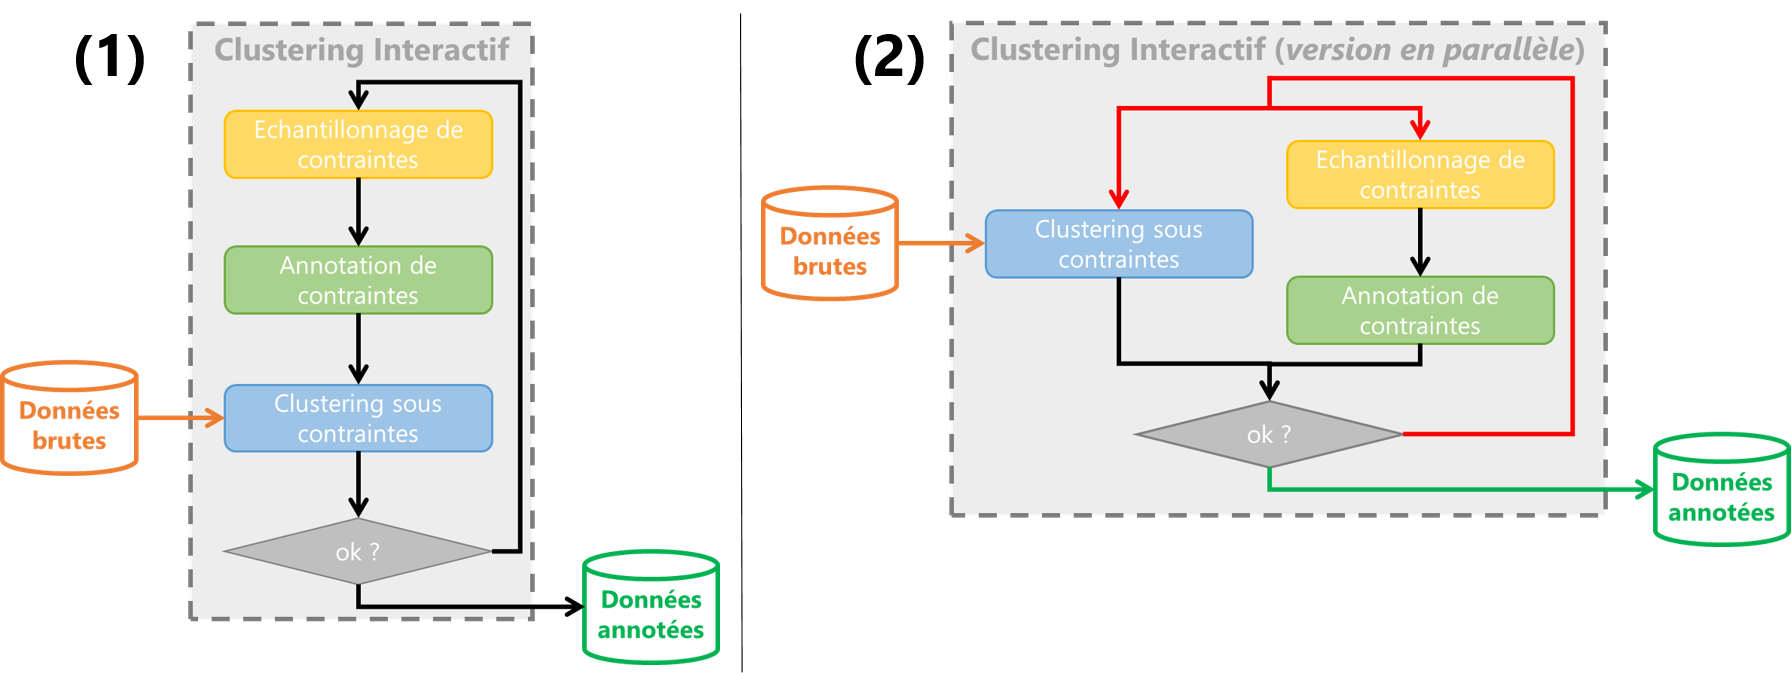
\includegraphics[width=0.95\textwidth]{figures/interactive-clustering-architecture-sequentielle-vs-parallele}
				\caption{
					Schéma comparatif des architectures du \textit{clustering} interactif : \textbf{(1)} représente la version séquentielle initialement présentée en \textsc{Chapitre~\ref{chapter:3-CLUSTERING-INTERACTIF}} où le \textit{clustering} s'adapte avec les annotation de l'itération en cours ; \textbf{(2)} représente l'évolution en mode \textit{parallèle} où le \textit{clustering} s'adapte avec les annotations de l'itération précédente (décalage d'une itération).
				}
				\label{figure:4.3.4-ETUDE-COUT-TOTAL-ARCHITECTURE}
			\end{figure}
			
			% Equation : Adaptation du Temps pour une itération (parallèle).
			Avec cette version, le temps nécessaire à une itération correspond à la durée la plus longue entre le temps d'annotation et le temps de calcul des algorithmes.
			Nous pouvons donc adapter l'\textsc{Equation~\ref{equation:4.3.4-ETUDE-COUT-UNE-ITERATION-SEQUENTIELLE}} par l'équation suivante :
			\begin{equation}
				\label{equation:4.3.4-ETUDE-COUT-UNE-ITERATION-PARALLELE}
				\begin{cases}
					% Computation time.
					\texttt{computation\_time}~[s]&
						~\propto~0.17 \cdot \texttt{dataset\_size}\\
					% Annotation time.
					\texttt{annotation\_time}~[s]&
						~\propto~7.8 \cdot \texttt{batch\_size} \\
					% One iteration time (parallel).
					\texttt{iteration\_time(parallel)}~[s]&
						~\propto~max(\texttt{computation\_time}, \texttt{annotation\_time}) \\
				\end{cases}
			\end{equation}
			
			% Equation : Adaptation du Nombre d'itérations (parallèle).
			Ensuite, afin de limiter les pertes de temps (humain et machine), nous pouvons choisir une taille de lot d'annotation rendre les deux durées équivalentes.
			Nous déduisons donc les changements suivants dans l'\textsc{Equation~\ref{equation:4.3.4-ETUDE-COUT-NOMBRE-ITERATIONS-SEQUENTIEL}} :
			\begin{equation}
				\label{equation:4.3.4-ETUDE-COUT-NOMBRE-ITERATIONS-PARALLELE}
				\begin{cases}
					% Batch size.
					\texttt{optimal\_batch\_size}~[\#]&
						~\propto~\frac{\texttt{computation\_time}}{7.8}
						~\propto~0.0218 \cdot \texttt{dataset\_size} \\
					% Iterations number.
					\texttt{iterations\_needed}~[\#] &
						~\propto~\frac{\texttt{nb\_constraints}}{\texttt{optimal\_batch\_size}}
						~\propto~144.5 \\
				\end{cases}
			\end{equation}
			
			% Equation: Adaptation du Temps total pour un projet (parallèle).
			Enfin, il suffit de combiner \textsc{Equation~\ref{equation:4.3.4-ETUDE-COUT-UNE-ITERATION-PARALLELE}} et \textsc{Equation~\ref{equation:4.3.4-ETUDE-COUT-NOMBRE-ITERATIONS-PARALLELE}} pour estimer le temps total nécessaire à un projet d'annotation pour converger vers $90$\% de \texttt{v-measure} utilisant la version parallèle du \textit{clustering} interactif :
			\begin{equation}
				\label{equation:4.3.4-ETUDE-COUT-TOTAL-PARALLELE}
				\begin{cases}
					% Total time (parallel).
					\texttt{total\_time(parallel)}~[s] &
						~\propto~\texttt{iteration\_time} \cdot \texttt{iterations\_needed} \\
					\texttt{total\_time(parallel)}~[s] &
						~\propto~24.6 \cdot \texttt{dataset\_size}
				\end{cases}
			\end{equation}
			
			% Figure.
			Ces estimations mises à jour sont représentées sur la \textsc{Figure~\ref{figure:4.3.4-ETUDE-COUT-TOTAL}} en fonction de plusieurs taille de jeu de données, et permettent de faire la comparaison avec la version séquentielle initialement présentée.
			
			% Figures.
			%
			\begin{figure}[!htb]
				\centering
				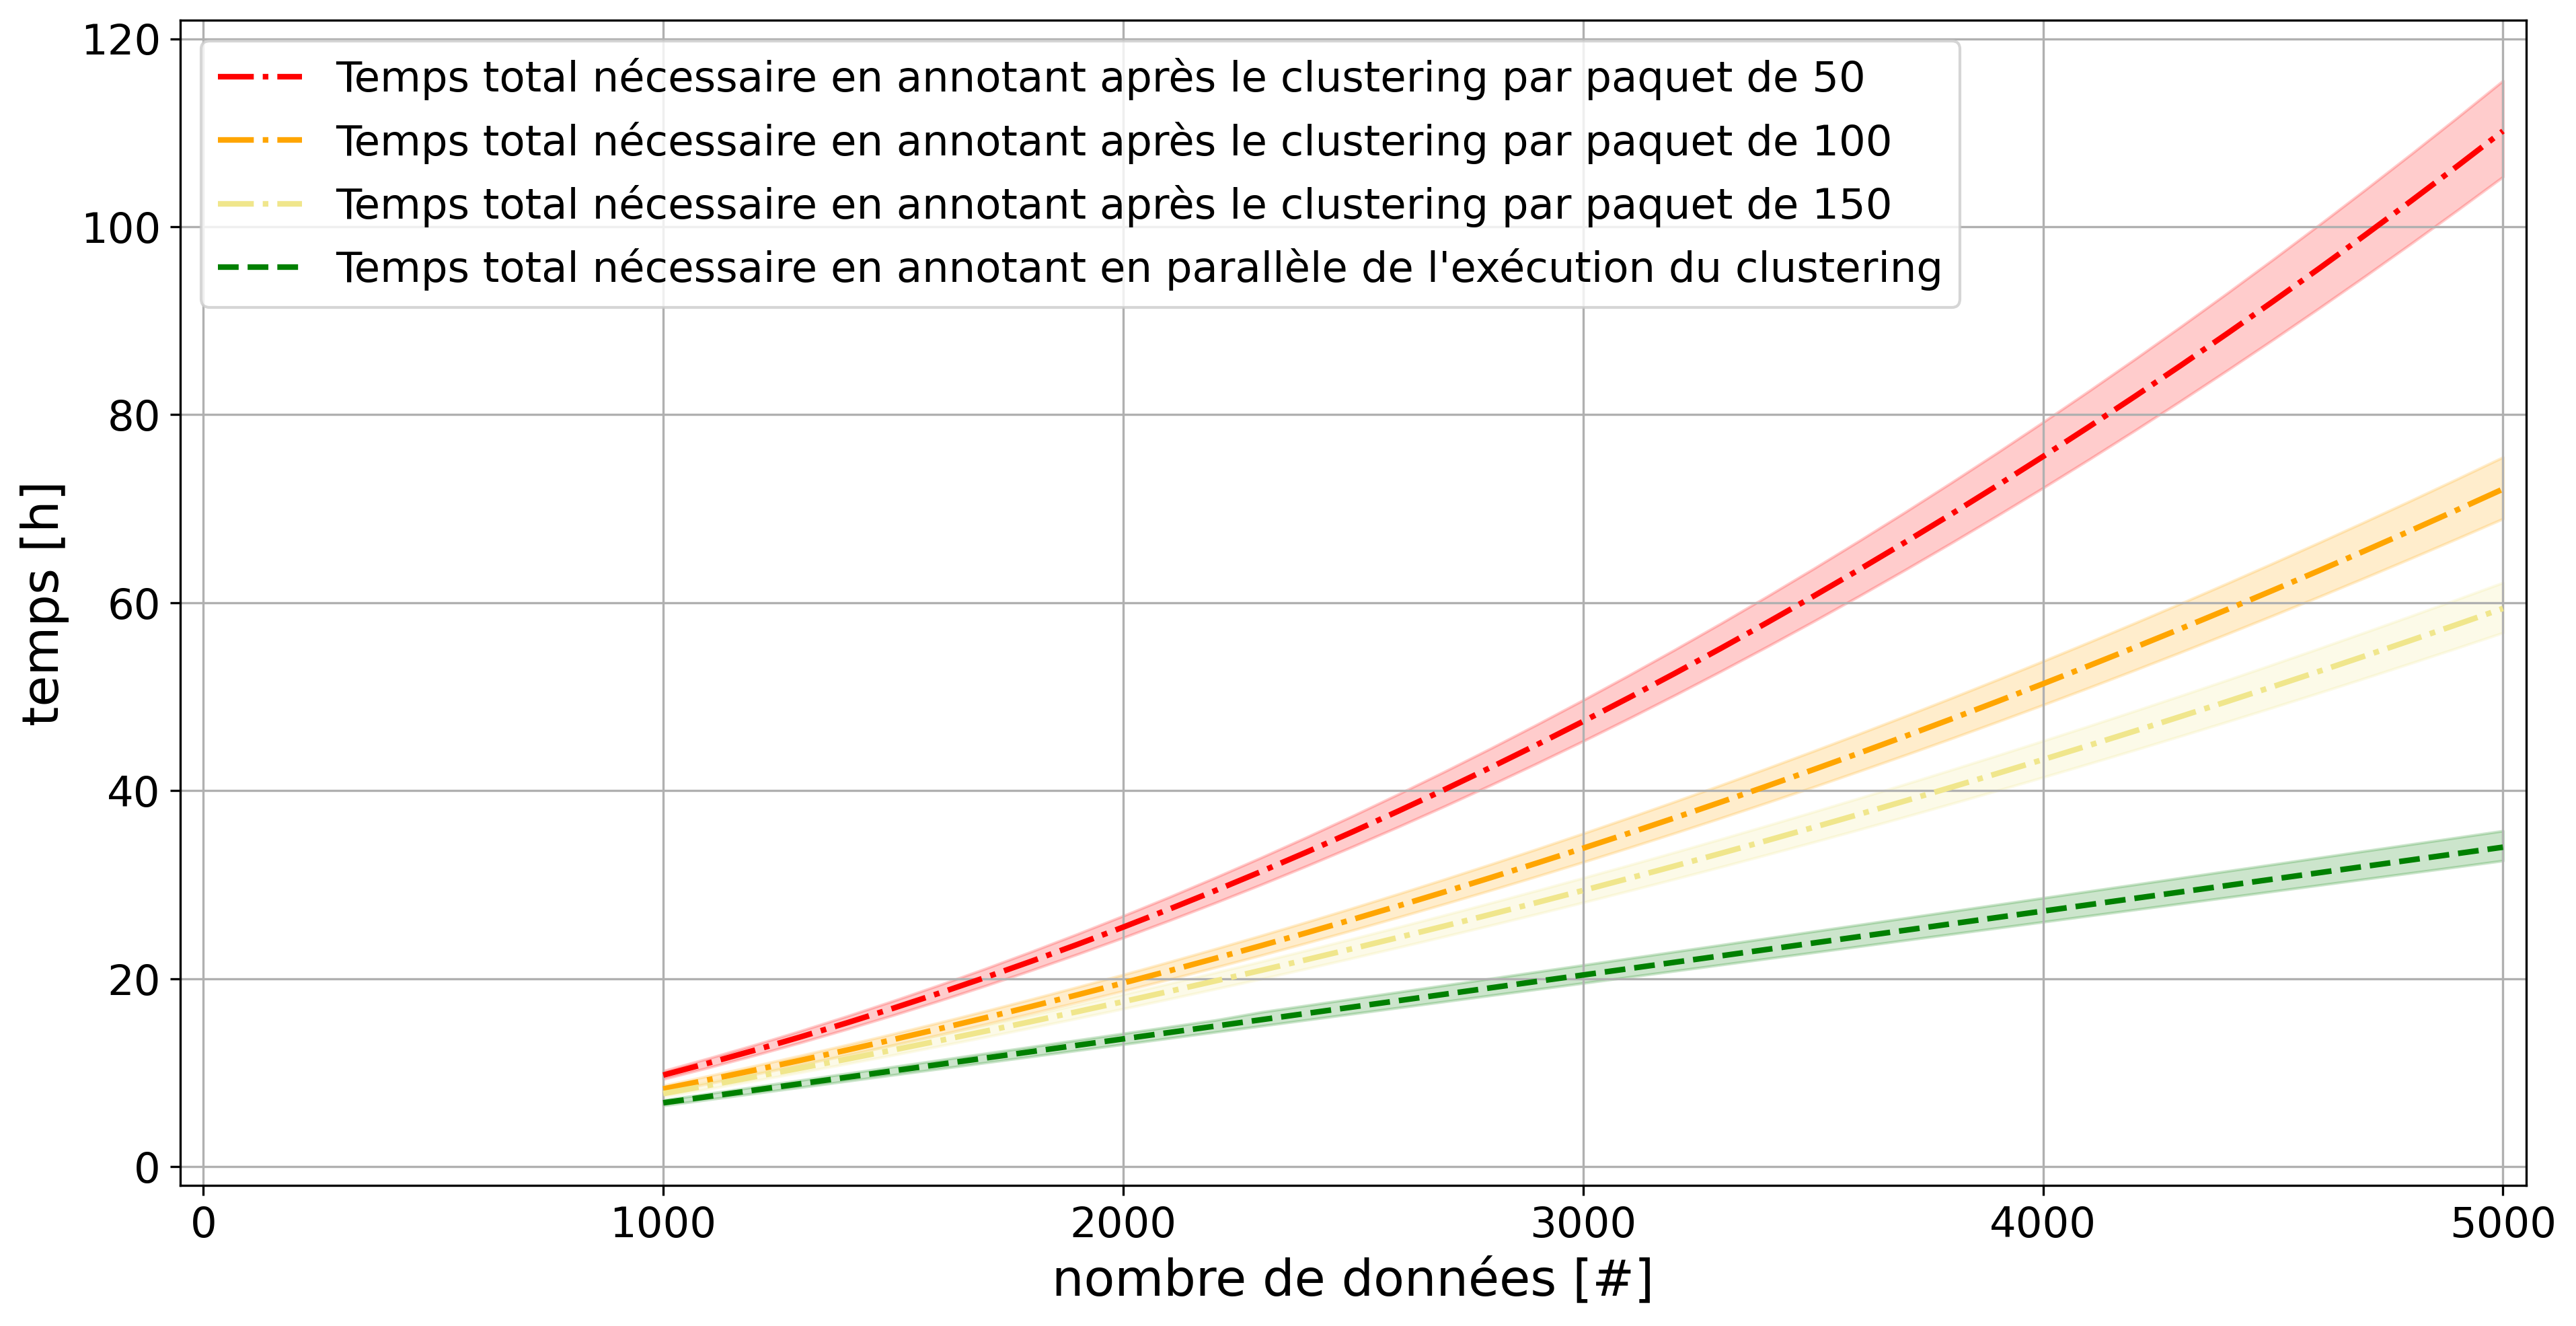
\includegraphics[width=0.95\textwidth]{figures/etude-temps-total-2-modelisation-parallele}
				\caption{
					Estimation du temps total nécessaire (en heures) pour modéliser un jeu de données avec notre \textbf{paramétrage favori} du \textit{clustering} interactif afin d'obtenir une annotation partielle (\textit{atteindre une \texttt{v-measure} de $90$\%}), en fonction de plusieurs taille de jeu de données, plusieurs tailles de lots d'annotation, et mettant en opposition l'approche séquentielle (\textit{annotation puis le clustering}) et l'approche parallèle (\textit{annotation pendant le clustering}).
				}
				\label{figure:4.3.4-ETUDE-COUT-TOTAL}
			\end{figure}
			
			% Résultats et discussion : linéaire, 25 x dataset size : c'est acceptable !
			Nous pouvons déjà remarquer que le coût d'annotation du projet devient linéaire en nombre de données (pente de $24.6$ secondes) et nécessite un nombre fixe de $145$ itérations.
			En reprenant une base de $5~000$ données et une marge de $2$ jours pour corriger et nommer les \textit{clusters}\footnote{
				voir. \textsc{Algorithme~\ref{algorithm:3.2-CLUSTERING-INTERACTIF}}, \textit{ligne 13}.
			}, cela représente $4.8$ {\footnotesize $(+2)$} jours de travail, un estimation équivalente à une annotation traditionnelle qui nécessite $5 $ {\footnotesize $(+2)$} jours de travail d'après nos approximations.
			De plus, si nous ajoutons des plusieurs opérateurs, cette version parallèle reste compétitive (\textit{avec $2$ annotateurs : $2.5$ {\footnotesize $(+2)$} jours vs $3$ {\footnotesize $(+2)$} jours ; avec $4$ annotateurs : $1.3$ jours vs $2$ {\footnotesize $(+2)$} jours}).
			Cette découverte est très encourageante, car cela confirme qu'une méthodologie basée sur notre implémentation du \textit{clustering} interactif \textbf{permet d'obtenir une base d'apprentissage avec un coût temporel équivalent à un projet traditionnel} utilisant une annotation par label.
			Cette méthode est d'autant plus intéressante qu'elle fait intervenir un mécanisme d'annotation rapide et intuitif pour un expert métier.
			
			% Conclusion.
			\begin{leftBarSummary}
				Au cours de cette étude de coûts, nous avons pu déduire que :
				\begin{itemize}
					\item[\itemok] L'annotation d'une contrainte nécessite en moyenne $8$ secondes : cette tâche est rapide et intuitive (cf. \textsc{Section~\ref{section:4.3.1-ETUDE-COUTS-TEMPS-ANNOTATION}}) ;
					\item[\itemok] Notre paramétrage favori, permettant d'atteindre $90$\% de \texttt{v-measure} avec un coût minimal, est constitué du prétraitement simple (\texttt{prep.simple}), de la vectorisation TF-IDF (\texttt{vect.tfidf}), du \textit{clustering} KMeans avec modèle COP (\texttt{clust.kmeans.cop}) et de l'échantillonnage des données les plus proches dans des clusters différents (\texttt{sampl.closest.diff}). Ce paramétrage a un coût moyen de $0.17 \cdot \texttt{dataset\_size}$ secondes (cf. \textsc{Section~\ref{section:4.3.2-ETUDE-COUTS-TEMPS-CALCUL}}) ;
					\item[\itemok] Une adaptation optimale de notre méthodologie consiste à paralléliser l'exécution du \textit{clustering} et l'annotation de contraintes afin de limiter les temps d'attente inutiles. Une telle méthode a un coût moyen de $24.6 \cdot \texttt{dataset\_size}$ pour atteindre $90$\% de \texttt{v-measure}, auquel on ajoute $2$ jours de travail pour raffiner les clusters et les nommer. Ce temps est compétitif à une annotation traditionnelle (cf. \textsc{Section~\ref{section:4.3.4-ETUDE-COUTS-TOTAL}}) ;
					\item[\itemok] Cette étude met en avant l'intérêt des interactions homme-machine : (1) l'expert métier se recentre sur son domaine de compétence avec une caractérisation proche de ses connaissances ("\textit{les données sont-elles similaires ?}") et (2) la machine optimise l'intervention de l'expert pour que ce dernier soit toujours pertinent dans ses contributions.
				\end{itemize}
			\end{leftBarSummary}
		
		% Transition: Vers Pertinence et Rentabilité.
		Dans les sections suivantes, nous allons nous intéressé à l'analyse des résultats de cette méthode.
		En effet, en situation réelle, nous n'avons pas accès à la vérité terrain car elle est justement en cours de construction.
		Il nous est donc impossible d'estimer notre seuil de \texttt{v-measure}, et donc incapable de s'arrêter à $90$\% de \texttt{v-measure}.
		Nous nous intéressons donc à l'estimation de la valeur métier d'un résultat de \textit{clustering} (cf. hypothèse de pertinence en \textsc{Section~\ref{section:4.4-HYPOTHESE-PERTINENCE}}) et à la définition de cas d'arrêt agnostique d'une vérité terrain (cf. hypothèse de rentabilité en \textsc{Section~\ref{section:4.5-HYPOTHESE-RENTABILITE}}).
	
	
	%%%%%--------------------------------------------------------------------
	%%%%% Section 4.4: Hypothèse de pertinence.
	%%%%%--------------------------------------------------------------------
	\newpage
	\section{Évaluation de l'hypothèse de pertinence}
\label{section:4.4-HYPOTHESE-PERTINENCE}

	%%% Introduction / Transition.
	Jusqu'à présent, nous avons analysé la performance et l'évolution des résultats de notre implémentation du \textit{clustering} interactif à l'aide d'une vérité terrain (cf. calcul de \texttt{v-measure}).
	Cependant, une telle référence n'est pas accessible en situation réelle (l'objectif de notre méthode est précisément de la construire).
	Nous devons donc nous intéresser à d'autres moyens d'estimer la pertinence des bases d'apprentissages obtenus et de définir comment définir l'exploitabilité d'un résultat.
	Ainsi, nous aimerions vérifier l'hypothèse suivante :
	
	%%% Formulation des hypothèses:
	\begin{tcolorbox}[
		title=\faVial~\textbf{Hypothèse de pertinence}~\faVial,
		colback=colorTcolorboxHypothesis!15,
		colframe=colorTcolorboxHypothesis!75,
		width=\linewidth
	]
		« \textbf{
			Au cours d'une méthodologie d'annotation basée sur le \textit{clustering} interactif, il est possible à un expert métier d'évaluer rapidement la pertinence de la base d'apprentissage en construction sans utiliser de vérité terrain.
		} » \\
		
		% Figure.
		La \textsc{Figure~\ref{figure:4.4-HYPOTHESE-PERTINENCE}} illustre cette hypothèse et l'espoir de pouvoir caractériser la qualité de la base d'apprentissage en cours de construction en fonction d'une valeur métier exprimée par un expert.
		%
		\begin{figure}[H]  % keep [H] to be in the tcolorbox.
			\centering
			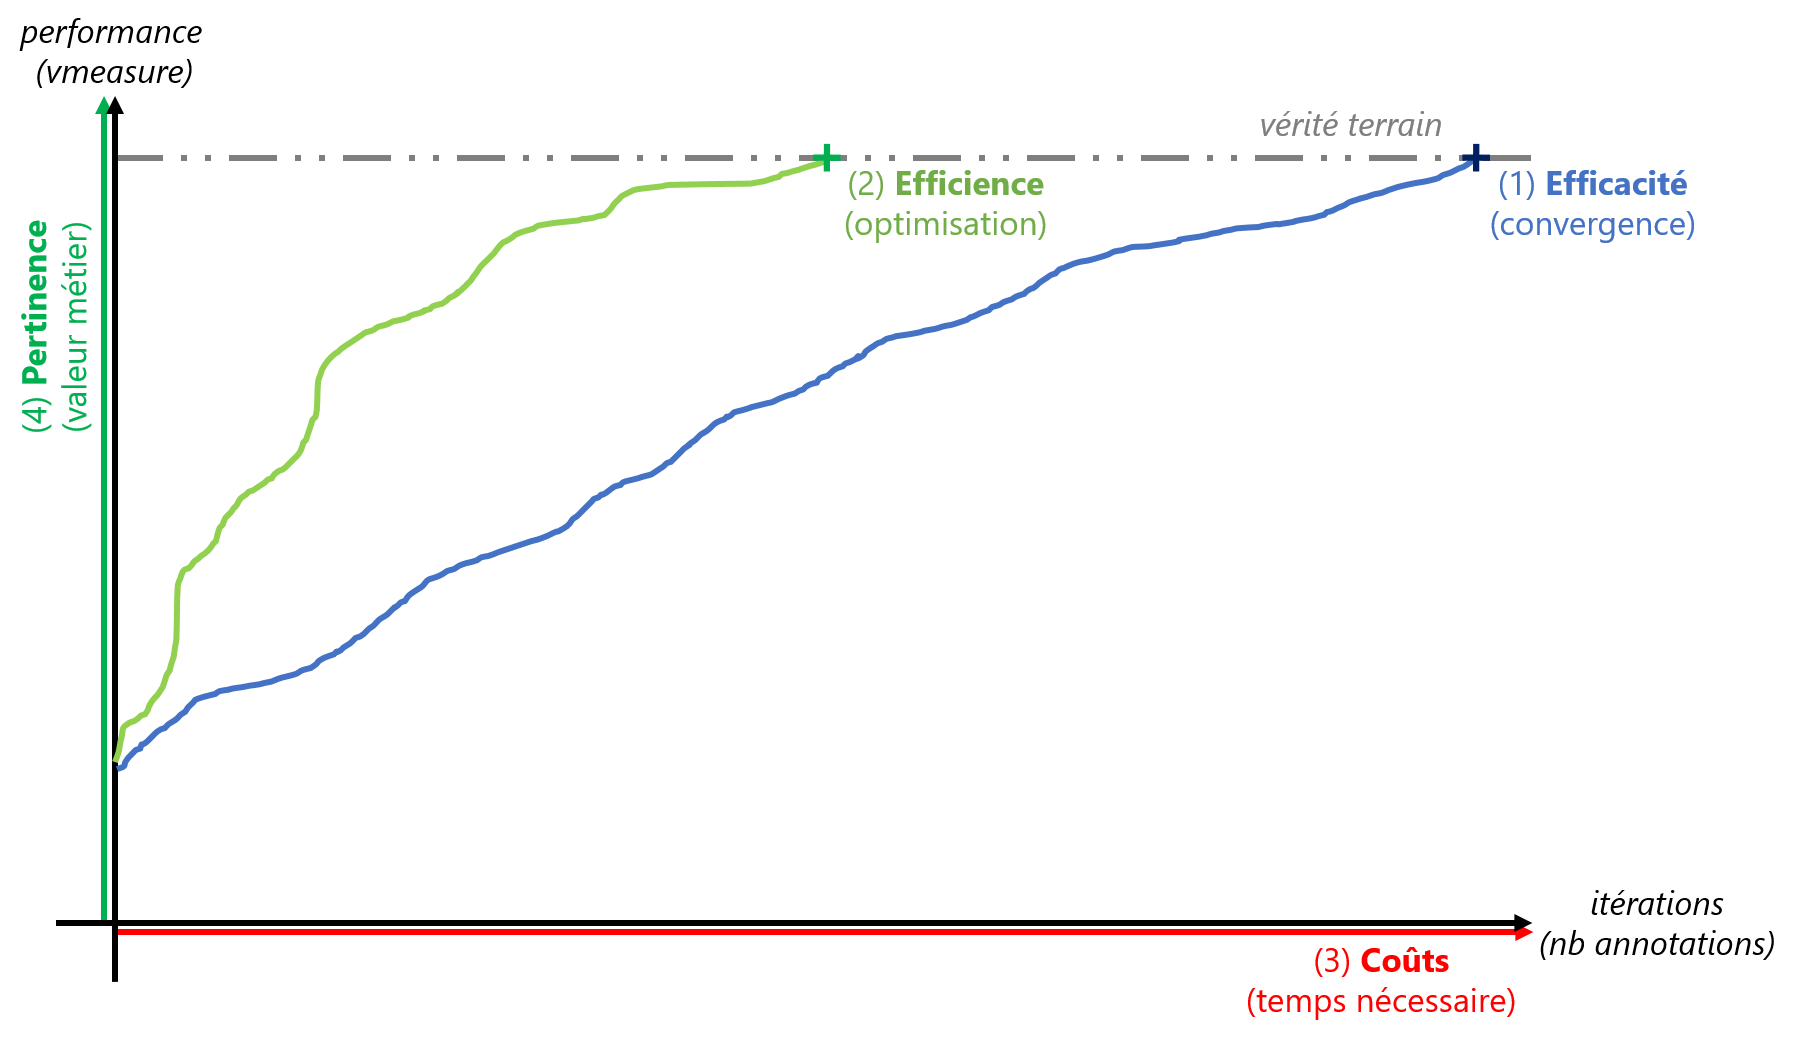
\includegraphics[width=0.95\textwidth]{figures/hypotheses-04-pertinence}
			\caption{Illustration des études réalisées sur le \textit{clustering} interactif (\textit{étape 4/6}) en schématisant l'évolution de la pertinence (\textit{valeur métier évaluée par l'expert et exprimé en nombre de clusters}) d'une base d'apprentissage en cours de construction en fonction du coût temporel de la méthode (\textit{temps nécessaire à l'expert métier et à la machine}).}
			\label{figure:4.4-HYPOTHESE-PERTINENCE}
		\end{figure}

	\end{tcolorbox}
		
	% Résumé de l'étude.
	Afin de vérifier cette hypothèse, nous explorons trois approches :
	\begin{itemize}
		\item une \textbf{vérification par un expert} du partitionnement des données obtenus, en parcourant manuellement le contenu des \textit{clusters} et en donnant un avis sur l'exploitabilité de ces derniers (cf. \textsc{Section~\ref{section:4.4.1-ETUDE-PERTINENCE-VERIFICATION-MANUELLE}}) ;
		\item une analyse des \textbf{patterns linguistiques saillants} dans la base d'apprentissage à l'aide d'une stratégie de sélection des composantes principales d'un modèle (cf. \textsc{Section~\ref{section:4.4.2-ETUDE-PERTINENCE-PATTERNS-LINGUISTIQUES}}),
		\item et une approche utilisant un \textbf{résumé automatique de thématique} par un modèle de langue, permettant de décrire succinctement le contenu des \textit{clusters} en une phrase. (cf. \textsc{Section~\ref{section:4.4.3-ETUDE-PERTINENCE-RESUME-AUTOMATIQUE}}).
	\end{itemize}
	
	
	%%%
	%%% Subsection 4.4.1: Étude d'une vérification manuelle de la valeur métier d'une base d'apprentissage par un expert
	%%%
	\subsection{Étude d'une vérification manuelle et non assistée de la valeur métier d'une base d'apprentissage par un expert}
	\label{section:4.4.1-ETUDE-PERTINENCE-VERIFICATION-MANUELLE}
		
		% Objectif de l'expérience.
		Afin d'estimer la pertinence d'un résultat de \textit{clustering}, notre première intuition consiste à demander simplement l'avis d'un expert sur la base d'apprentissage en cours de construction.
		En lui posant certaines questions, nous espérons obtenir une description qualitative de chaque \textit{cluster} et ainsi déduire quand le résultat du \textit{clustering} interactif devient exploitable pour définir et entraîner un modèle de classification.
	
		%%% Protocole expérimental.
		\subsubsection{Protocole expérimental}
			
			% Pseudo-code.
			Pour résumer le protocole expérimental que nous décrivons ci-dessous, vous pouvez vous référer au pseudo-code décrit dans \textsc{Algorithme~\ref{algorithm:4.4.1-ETUDE-PERTINENCE-VERIFICATION-MANUELLE-PROTOCOLE}]}.
			%
			\begin{algorithm}[!htb]
				\begin{algorithmic}[1]
					\Require jeux de données annotés (vérité terrain) de tailles différentes
					\State \textbf{initialisation (données)}: récupérer ou générer les données et la vérité terrain
					\State \textbf{initialisation (contraintes)}: créer une liste vide de contraintes
					\State \textbf{prétraitement}: supprimer le bruit dans les données avec \texttt{prep.simple}
					\State \textbf{vectorisation}: transformer les données en vecteurs avec \texttt{vect.tfidf}
					\State \textbf{clustering initial}: regrouper les données par similarité avec \texttt{clust.kmeans.cop}
					\State \textbf{évaluation manuelle}: juger de l'exploitabilité de chaque \textit{cluster}
					\Repeat
						\State \textbf{échantillonnage}: sélectionner de nouvelles contraintes à annoter
						\State \textbf{simulation d'annotation}: ajouter des contraintes avec \texttt{samp.closest.diff}
						\State \textbf{clustering}: regrouper les données par similarité avec \texttt{clust.kmeans.cop}
						\State \textbf{évaluation manuelle}: juger de l'exploitabilité de chaque \textit{cluster}
						\State \textbf{labellisation manuelle}: nommer chaque \textit{cluster} exploitable
					\Until{annotation de toutes les contraintes possibles}
					\State \textbf{analyse}: afficher l'évolution de l'exploitabilité de chaque itération de \textit{clustering}
					\Ensure discussion sur la complexité de la tâche et sur l'évolution de l'exploitabilité
				\end{algorithmic}
				\caption{Description en pseudo-code du protocole expérimental de l'étude de vérification manuelle non assistée de la valeur métier d'une base d'apprentissage.}
				\label{algorithm:4.4.1-ETUDE-PERTINENCE-VERIFICATION-MANUELLE-PROTOCOLE}
			\end{algorithm}
			
			% Description de la vérité terrain.
			Nous utilisons comme vérité terrain le jeu de données \texttt{Bank Cards (v1.0.0)} : ce dernier traite des demandes les plus fréquentes des clients en ce qui concerne la gestion de leur carte bancaire.
			Il est composé de $500$ questions rédigées en français et réparties en $10$ classes (\texttt{perte ou vol de carte}, \texttt{carte avalée}, \texttt{commande de carte}, ...).
			Pour plus de détails, consultez l'annexe~\ref{annex:C.1-DATASET-BANK-CARDS}.
			
			% Description des tentatives de la méthode.
			Sur ce jeu de données, nous exécutons une tentative complète
			\footnote{Tentative complète : itérations d'échantillonnage, d'annotation et de \textit{clustering} jusqu'à annotation de toutes les contraintes possibles.}
			de la méthode du \textit{clustering} interactif utilisant notre paramétrage favori, et cette tentative est répétée $5$ fois pour contrer les aléas statistiques des exécutions.
			
			% Description de l'évaluation manuelle.
			Au cours des itérations, un expert qualifie chaque \textit{cluster} en donnant son avis sur sa valeur métier.
			Afin d'encadrer ses réponses, nous lui demandons d'analyser trois aspects :
			\begin{itemize}
				\item est-ce que le \textit{cluster} a une thématique principale \textbf{bien définie} ? (\textit{en effet, comment interpréter un cluster sans définition claire ?})
				\item est-ce que le \textit{cluster} est constitué par un nombre suffisant de données ? (\textit{en effet, comment entraîner un modèle de classification sans données ?})
				\item est-ce que le \textit{cluster} n'est pas trop bruité ? (\textit{en effet, comment avoir de bonnes performances si la base d'apprentissage n'est pas fiable ?})
			\end{itemize}
			
			L'avis exprimé par l'expert métier est alors classé en trois niveaux :
			\begin{itemize}
				\item \textbf{exploitable} : le \textit{cluster} possède (1) une thématique bien définie, (2) un nombre de données suffisant pour entraîner un modèle de classification et (3) peu de bruit ; ce \textit{cluster} peut donc être exploité en l'état ou avec peu de modifications manuelles ;
				\item \textbf{partiellement exploitable} : soit le \textit{cluster} est composé de plusieurs de thématiques (\textit{deux ou trois}), soit il ne comporte pas pas assez de données (\textit{moins d'une vingtaines}), soit il est bruité (\textit{au moins un quart de bruit}) ; ce \textit{cluster} donne une première base pour créer une classe, mais un travail manuel est nécessaire (\textit{ajout de données, tri du bruit, ...}) ;
				\item \textbf{non exploitable} : soit le \textit{cluster} ne contient pas ou contient trop de thématique, soit c'est un \textit{cluster} singleton ou un \textit{cluster} poubelle, soit ce \textit{cluster} est complètement bruité ; dans tous les cas, il n'est absolument pas exploitable sans un gros travail manuel.
			\end{itemize}
			
			Pour limiter la charge de travail de l'opérateur, nous ne demandons l'expertise que toutes les $5$ itérations d'une tentative.
			
			% Référence scripts.
			\begin{leftBarInformation}
				Les scripts de l'expérience, réalisés avec des \textit{notebooks} Python (\cite{van-rossum-drake:2009:python-reference-manual}), sont disponibles dans un dossier dédié de~\cite{schild:2021:cognitivefactory-interactiveclusteringcomparativestudy}.
			\end{leftBarInformation}
			

		%%% Résultats
		\subsubsection{Résultats obtenus}
			
			% Axiome/Contraintes.
			\begin{leftBarWarning}
				Par manque de personnes aptes à qualifier le jeu de données utilisé, les annotations réalisées dans cette étude n'ont pu être faites que par un seul annotateur.
				Malgré cette contrainte, nous supposons que la réalisation de l'analyse sur $5$ tentatives différentes de la méthode permet de limiter les biais et de discuter des tendances générales.
			\end{leftBarWarning}
		
			% Description statistiques.
			La \textsc{Figure~\ref{figure:4.4.1-ETUDE-PERTINENCE-VERIFICATION-MANUELLE}} met en avant l'évolution de le pertinence moyenne estimée par l'opérateur sur la base des contenu des \textit{clusters}.
			Nous allons nous intéresser à trois phases s'y distinguant.
			
			% 0: Initialisation
			À l'initialisation (itération $0$), la majeure partie des \textit{clusters} sont inexploitables (environ $60$\%) et seul $35$\% d'entre eux semblent exploitables.
			Dans le top $3$ des classes facilement identifiables à ce stade, nous retrouvons \texttt{gestion\_sans\_contact} ($5/5$), \texttt{consultation\_solde} ($3/5$) et \texttt{gestion\_carte\_virtuelle} ($3/5$).
			
			% 0-10: Phase d'exploration.
			Nous constatons ensuite une première phase de remaniement des \textit{clusters}, située entre les itérations $0$ et $10$, où le taux d'inexploitables chute au profit des \textit{clusters} partiellement exploitables, dont la proportion augmente de $10$ à près de $40$\%.
			À l'itération $10$, le top $3$ des classes identifiables mais bruitées ou en cohabitation dans un \textit{cluster} sont \texttt{gestion\_carte\_virtuelle} ($4/5$),  \texttt{alerte\_perte\_vol\_carte} ($4/5$) et  \texttt{commande\_carte} ($4/5$).
			
			% 10-25: Phase de consolidation.
			Une seconde phase de consolidation se présente entre les itérations $10$ et $25$.
			Durant cette phase, les taux de \textit{clusters} non exploitables et de partiellement exploitables diminuent alors que le taux d'exploitables monte en flèche (de $35$\% à $90$\% en $15$ itérations).
			La majeure partie des \texttt{clusters} sont ainsi exploitables en l'état ou après la correction de quelques points aberrants.
			Après l'itération $25$, le \textit{cluster} le plus récalcitrant concerne un mélange des classes \texttt{alerte\_perte\_vol\_carte} et \texttt{gestion\_decouvert} ($5/5$).

			% Figure.
			\begin{figure}[!htb]
				\centering
				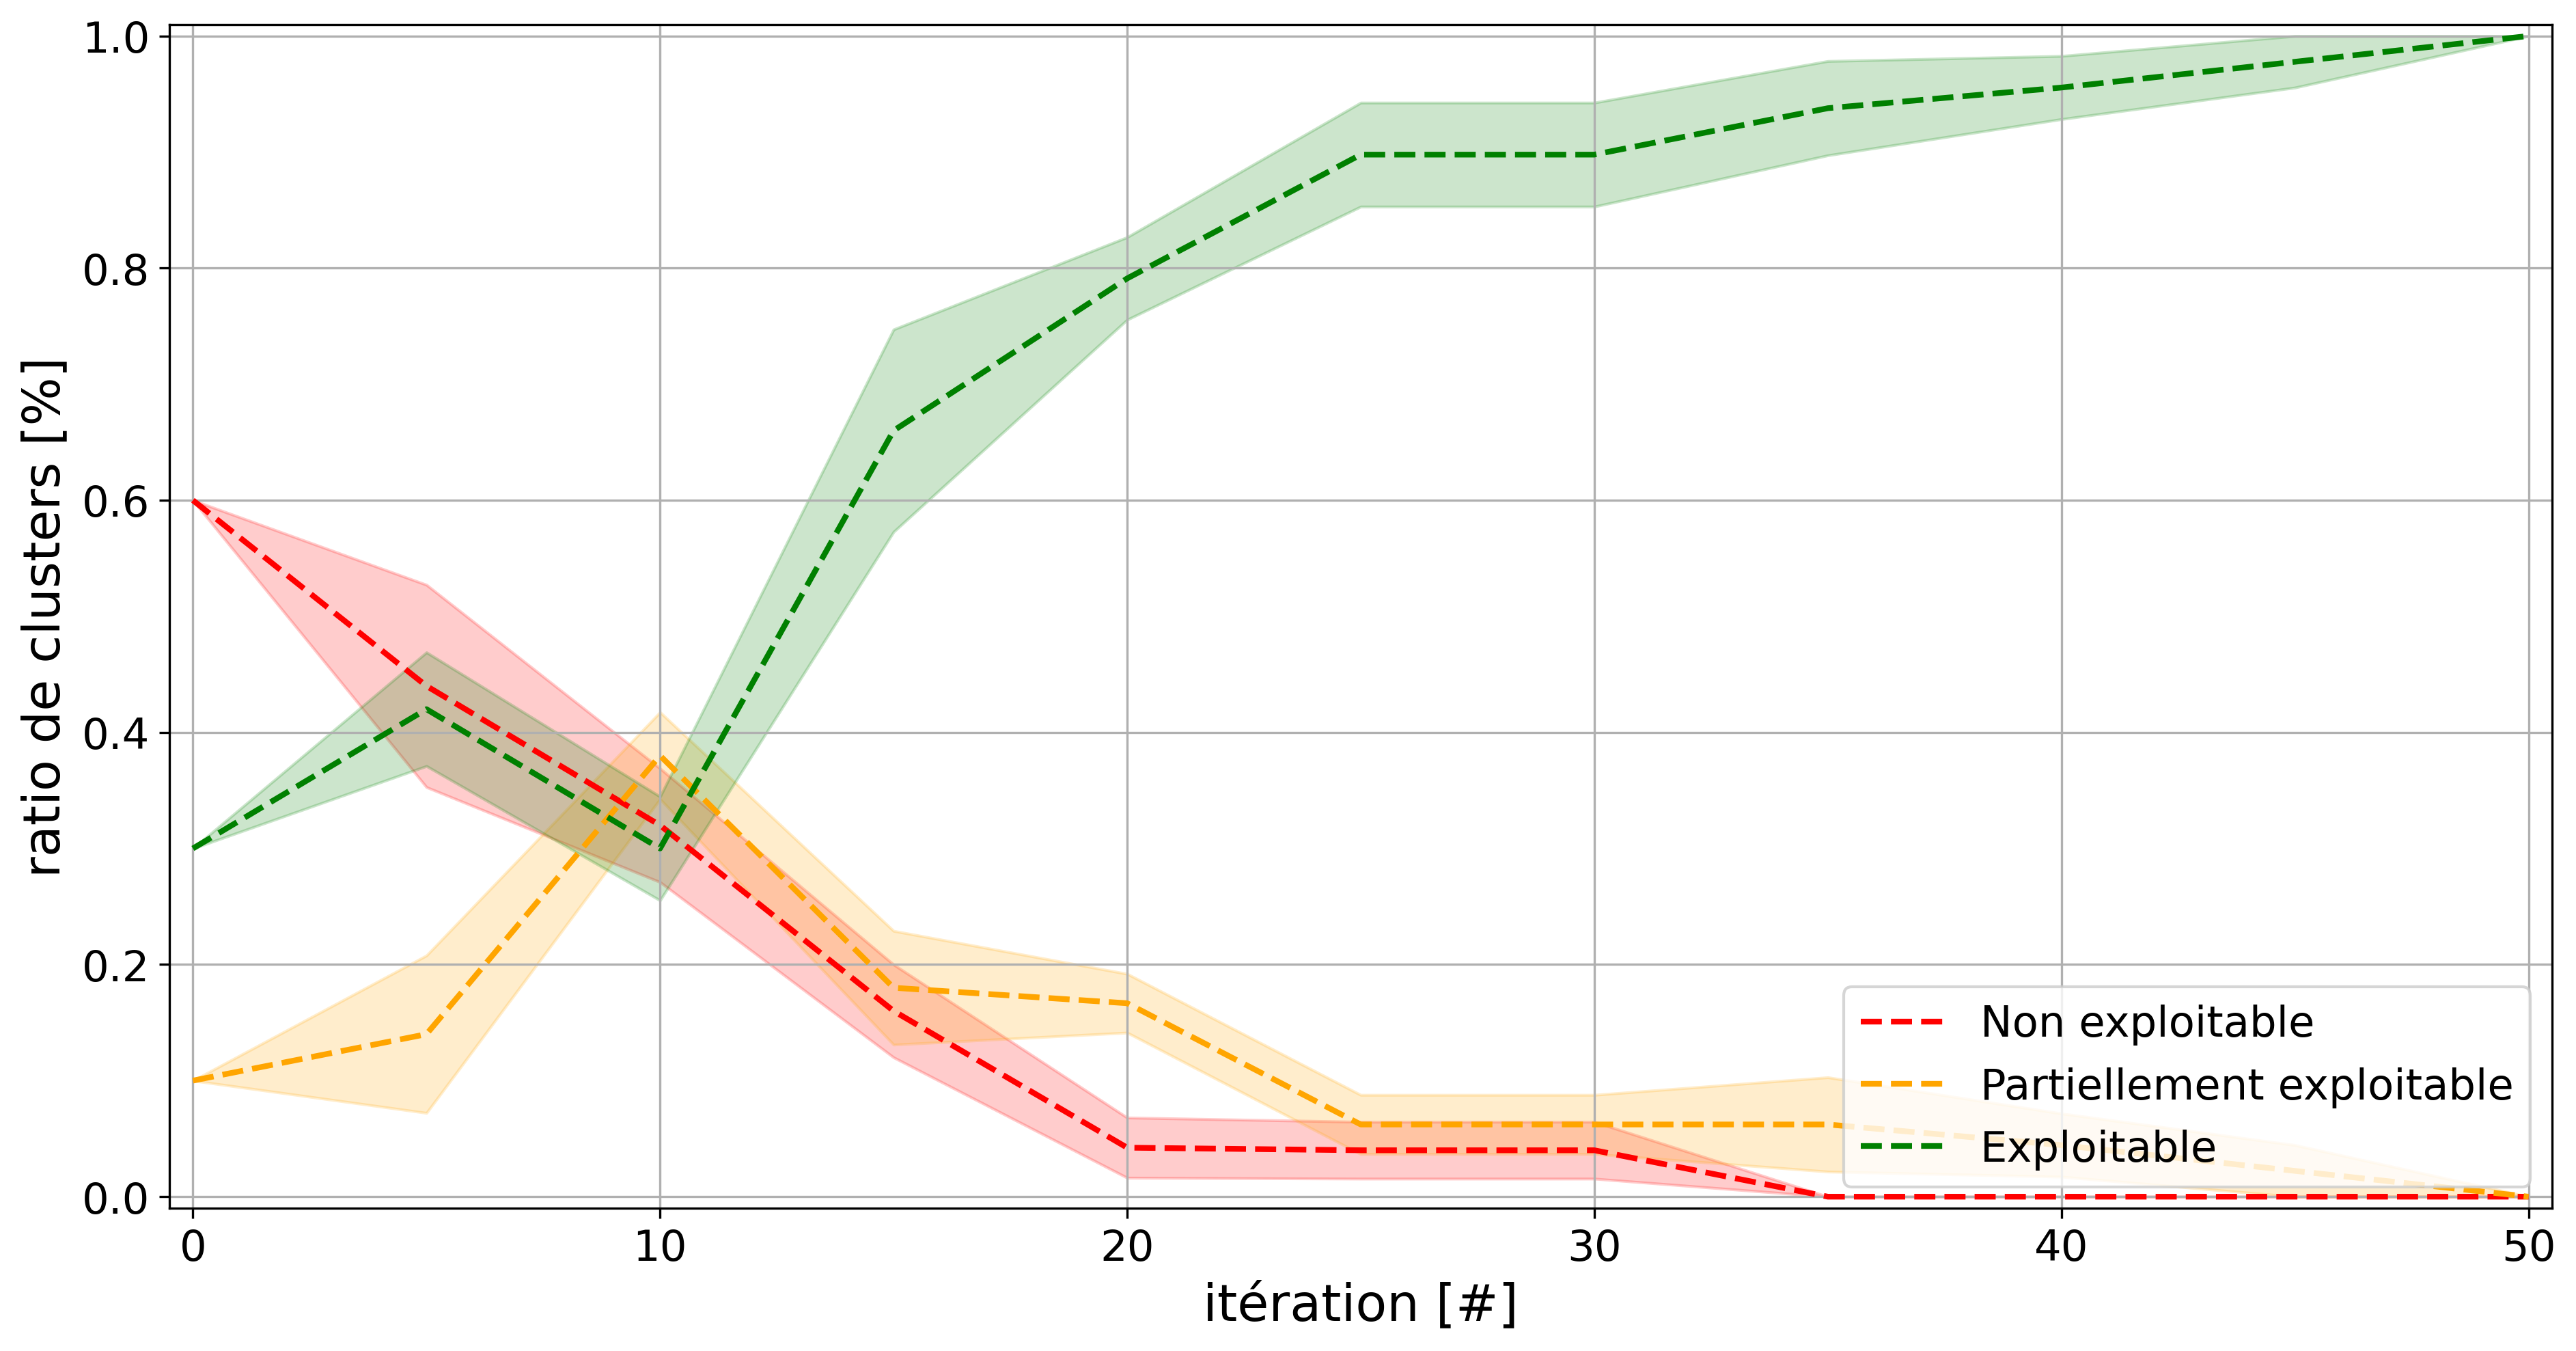
\includegraphics[width=0.95\textwidth]{figures/etude-pertinence-llm-check-clustering-annotation-favori}
				\caption{Évolution de la pertinence métier moyenne estimée manuellement au cours des itérations du résultat du \textit{clustering} interactif avec notre paramétrage favori.
				Cette pertinence, exprimée en proportion du nombre de \textit{clusters}, est retranscrite en trois niveaux : \texttt{exploitable} en vert, \texttt{partiellement exploitable} en orange, et \texttt{non exploitable} en rouge.}
				\label{figure:4.4.1-ETUDE-PERTINENCE-VERIFICATION-MANUELLE}
			\end{figure}


		%%% Discussion
		\subsubsection{Discussion}
		
			% Rappel de l'objectif.
			Cette première étude visait à observer comment un expert métier peut interpréter un résultat de \textit{clustering} proposé par notre méthode.
			
			% Remarques sur l'évolution de l'exploitabilité.
			Comme l'analyse n'a pu être faite que par un seul opérateur, nous ne nous attarderons pas sur la précision des taux d'exploitabilité des clusters.
			Nous pouvons déjà reconnaître que trois phases sont présentes :
			\begin{itemize}
				\item une première \textbf{phase exploratoire} (cf. itérations $0$ à $10$), où de premiers \textit{clusters} partiellement exploitables apparaissant.
				Ces derniers contiennent souvent une thématique bruitée ou quelques thématiques mal séparées, ce qui permet toutefois à l'expert de se faire une idée des thématiques contenu dans la collecte de données.
				Cependant, s'arrêter à ce stade demanderait beaucoup de travail manuel pour obtenir une base d'apprentissage opérationnelle ;
				\item une seconde \textbf{phase de consolidation} (cf. itérations $10$ à $25$), où les \textit{clusters} partiellement exploitable se raffinent.
				De plus en plus de \textit{clusters} bien définis naissent, avec une seul thématique et peu de bruits.
				Ces derniers pourraient être extraits et exploités en l'état ;
				\item une \textbf{phase de parachèvement} (cf. itérations après $25$), où la plupart des \textit{clusters} sont exploitables en l'état mais quelques-uns nécessitent encore du travail.
				Cette phase est la moins rentable car les derniers \textit{clusters} et points aberrants sont corrigés petit à petit, mais sans impact notable sur leur valeur métier. 
			\end{itemize}
			
			% Remaques expérience utilisateur : tâche complexe.
			Au cours de ces vérifications, il apparaît que la complexité réside dans l'analyse des \textit{clusters} partiellement exploitables.
			En effet, les clusters totalement exploitable ou totalement inexploitables sont souvent simples à identifier.
			les premiers se repèrent facilement, surtout quand ils sont déjà présents lors d'itérations précédentes (exemple de la classe \texttt{gestion\_sans\_contact}, présente dès l'itération $0$) ;
			les seconds, plutôt présents au début de la méthode, peuvent mélanger un grand nombre de thématique et s'apparenter rapidement à des \textit{clusters} poubelle.
			En revanche, les \textit{clusters} partiellement exploitables peuvent avoir des limites subjectives, alterant parfois l'avis de l'expert.
			
			% Remaques expérience utilisateur : tâche complexe.
			Pour aller plus loin, la difficulté de cette tâche est aussi dû aux contraintes suivantes :
			\begin{itemize}
				\item il faut être capable de maintenir en mémoire de grands ensembles de données ;
				\item il faut estimer la thématique principale à l'aide de données désordonnées ;
				\item il faut examiner la cohérence de cette thématique alors que le vocabulaire employé diffère ;
				\item il faut juger de l'importance du bruit contenu dans les \textit{clusters} ;
				\item il faut prendre du recul pour repérer la dispersion d'une thématique dans plusieurs \textit{clusters} ;
				\item ...
			\end{itemize}
			Tous ces facteurs peuvent donc nuire à la qualité, tant sur l'estimation de l'exploitabilité que sur le nommage des \textit{clusters}.
			
			% Remarques expérience utilisateur : impacts sur la qualité.
			Ainsi, nous déduisons aisément que l'expérience utilisateur proposée à l'expert métier n'est pas séduisante.
			Comme l'analyse de l'exploitabilité d'un \textit{cluster} semble être une tâche complexe, il semble inconcevable de demander sa réalisation sur tous les \textit{clusters} de toutes les itérations !
			De plus, sans aide supplémentaire et sans vis-à-vis pour se confronter à ses conclusions d'analyse, l'opérateur peut difficilement vérifier la cohérence et la reproductibilité de son travail.
			Il est donc nécessaire de considérer des pistes d'amélioration pour ne pas abandonner l'expert métier à lui-même dans cette tâche cruciale.
			
			% Conclusions et suggestion.
			Quelques pistes peuvent être étudiées pour accompagner l'opérateur :
			\begin{itemize}
				\item employer plusieurs experts pour valider par consensus leurs appréciation sur un résultat de \textit{clustering} : cette méthode est efficace pour rattraper les thématiques non identifiées et pour s'accorder sur la valeur d'un \textit{cluster} ;
				\item prémâcher le travail d'analyse en réalisant une étude linguistique des \textit{clusters}, et permettre ainsi d'identifier grossièrement les thématiques présentes en fonction du vocabulaire employé (cf. \textsc{Section~\ref{section:4.4.2-ETUDE-PERTINENCE-PATTERNS-LINGUISTIQUES}}) ;
				\item automatiser une partie du travail d'analyse en utilisant les capacités des larges modèles de langage (\textit{large language models}, \texttt{LLM}), afin d'alléger la charge de travail demandée aux experts métiers (cf. \textsc{Section~\ref{section:4.4.3-ETUDE-PERTINENCE-RESUME-AUTOMATIQUE}}).
			\end{itemize}
	
	
	%%%
	%%% Subsection 4.4.2: Etude des patterns linguistiques pertinents à l'aide de la \textit{Features Maximization}
	%%%
	\subsection{Étude des patterns linguistiques pertinents à l'aide de la Maximisation des Traits pour assister la vérification d'une base d'apprentissage}
	\label{section:4.4.2-ETUDE-PERTINENCE-PATTERNS-LINGUISTIQUES}
		
		% Objectif de l'expérience.
		Nous venons de conclure que la vérification manuelle d'un résultat de \textit{clustering} interactif est fonctionnelle, mais qu'elle souffre d'une très mauvaise expérience utilisateur.
		Afin d'améliorer cette aspect, une première idée consiste à mettre en valeur le vocabulaire caractéristique de chaque \textit{cluster} et d'examiner si ces informations sont utiles à l'appréciation de leur valeur métier.
	
		%%% Protocole expérimental.
		\subsubsection{Protocole expérimental}
			
			% Pseudo-code.
			Pour résumer le protocole expérimental adapté, vous pouvez vous référer au pseudo-code décrit dans \textsc{Algorithme~\ref{algorithm:4.4.2-ETUDE-PERTINENCE-PATTERNS-LINGUISTIQUES-PROTOCOLE}}.
			%
			\begin{algorithm}[!htb]
				\begin{algorithmic}[1]
					\Require jeux de données annotés (vérité terrain) de tailles différentes
					\State \textbf{initialisation (données)}: récupérer ou générer les données et la vérité terrain
					\State \textbf{initialisation (contraintes)}: créer une liste vide de contraintes
					\State \textbf{prétraitement}: supprimer le bruit dans les données avec \texttt{prep.simple}
					\State \textbf{vectorisation}: transformer les données en vecteurs avec \texttt{vect.tfidf}
					\State \textbf{clustering initial}: regrouper les données par similarité avec \texttt{clust.kmeans.cop}
					\State \textbf{évaluation manuelle}: juger de l'exploitabilité de chaque \textit{cluster}
					\Repeat
						\State \textbf{échantillonnage}: sélectionner de nouvelles contraintes à annoter
						\State \textbf{simulation d'annotation}: ajouter des contraintes avec \texttt{samp.closest.diff}
						\State \textbf{clustering}: regrouper les données par similarité avec \texttt{clust.kmeans.cop}
						\State \textbf{analyse linguistique}: déterminer le vocabulaire caractéristique de chaque cluster
						\State \textbf{évaluation semi-manuelle}: juger de l'exploitabilité de chaque \textit{cluster}
						\State \textbf{labellisation manuelle}: nommer chaque \textit{cluster} exploitable
					\Until{annotation de toutes les contraintes possibles}
					\State \textbf{analyse}: afficher l'évolution de l'exploitabilité de chaque itération de \textit{clustering}
					\Ensure discussion sur la complexité de la tâche et sur l'évolution de l'exploitabilité
				\end{algorithmic}
				\caption{Description en pseudo-code du protocole expérimental de l'étude des patterns linguistiques pertinents pour vérifier la valeur métier d'une base d'apprentissage.}
				\label{algorithm:4.4.2-ETUDE-PERTINENCE-PATTERNS-LINGUISTIQUES-PROTOCOLE}
			\end{algorithm}
			
			% Détails de l'expérience.
			Nous nous appuyons sur le même protocole que l'expérience précédente (cf. \textsc{Section~\ref{section:4.4.1-ETUDE-PERTINENCE-VERIFICATION-MANUELLE}}) : nous utilisons donc comme vérité terrain le jeu de données \texttt{Bank Cards (v1.0.0)}, nous réalisons $5$ tentatives complètes de la méthode du \textit{clustering} interactif utilisant notre paramétrage favori, et nous demandons toutes les $5$ itérations à un expert de qualifier les \textit{clusters} obtenus entre trois catégories (\textbf{exploitable}, \textbf{partiellement exploitable} et \textbf{non exploitable}).
			
			% Ajout de l'analyse linguistique.
			Cependant, avant de demander l'avis de l'expert, nous réalisons une analyse du vocabulaire employé.
			Pour cela, nous utilisons une sélection des patterns linguistiques pertinents basée sur la maximisation des traits (notée \texttt{FMC}, cf.~\cite{lamirel-etal:2017:novel-approach-feature}) : cette méthode permet de trouver les composantes vectorielle caractéristiques et discriminantes de chaque \textit{cluster} en attribuant un score à chaque couple $(\texttt{cluster}, \texttt{composante})$.
			Dans notre cas, en utilisant une vectorisation basée sur la fréquence du vocabulaire dans un document comme \textbf{TF-IDF} (\cite{sparck-jones:1972:statistical-interpretation-term}), nous pouvons déterminer les mots les plus représentatif de chaque \textit{cluster}.
			Ainsi, nous pouvons à la fois décrire chaque groupe de questions par une liste de mots clés caractéristiques, mais aussi surligner ces mots dans les questions à parcourir pour attirer l'attention de l'expert sur ce qui semble être statistiquement discriminant.
			
			% Description de l'évaluation semi-manuelle.
			Nous adaptons aussi la tâche de l'expert afin qu'il donne son avis sur chaque \textit{cluster} en répondant aux questions suivantes :
			\begin{itemize}
				\item est-ce que la liste des patterns linguistiques caractéristiques du \textit{cluster} est suffisamment complète pour permettre d'identifier une thématique principale \textbf{bien définie} ? (\textit{en effet, comment interpréter un cluster sans définition claire ?})
				\item est-ce que la liste des patterns linguistiques caractéristiques du \textit{cluster} identifie plusieurs thématiques ou bruits dans le \textit{cluster} ? (\textit{en effet, comment avoir de bonnes performances si la base d'apprentissage n'est pas fiable ?})
			\end{itemize}
			
			\begin{leftBarIdea}
				Nous pourrions aussi analyser l'impact ergonomique qu'apporte la mise en exergue des patterns linguistiques pertinents dans le texte de chaque \textit{cluster}.
				Une telle étude pourrait ainsi mesurer le gain de temps et de qualité par rapport à une vérification manuelle non assistée comme présentée en \textsc{Section~\ref{section:4.4.1-ETUDE-PERTINENCE-VERIFICATION-MANUELLE}}.
			\end{leftBarIdea}
			
			% Référence scripts.
			\begin{leftBarInformation}
				Les scripts de l'expérience, réalisés avec des \textit{notebooks} Python (\cite{van-rossum-drake:2009:python-reference-manual}), sont disponibles dans un dossier dédié de~\cite{schild:2021:cognitivefactory-interactiveclusteringcomparativestudy}.
				L'implémentation de la maximisation des traits est accessible ici dans~\cite{schild:2023:cognitivefactory-featuresmaximizationmetric}.
			\end{leftBarInformation}

		%%% Résultats
		\subsubsection{Résultats obtenus}
			
			% Axiome/Contraintes.
			\begin{leftBarWarning}
				Par manque de moyen, la relecture manuelle des \textit{clusters} n'a pas été réalisée.
				Nous présentons donc simplement quelques exemples d'analyses linguistiques réalisées grâce à la \texttt{FMC}.
			\end{leftBarWarning}
			
			% Description de deux cas d'études.
			Prenons quelques \textit{clusters} et suivons l'évolution de leur analyse linguistiques au cours des itérations.
			Nous nous référons aux tableaux ci-contre pour connaître le top $10$ des termes caractéristiques des différents \textit{clusters} ainsi qu'un extrait de questions issu de ces \textit{clusters} avec une mise en évidence des termes caractéristiques dans le texte.
			
			% Exemple d'un cluster qui est bien formé dès le début.
			D'abord, prenons l'exemple suivi dans la \textsc{Table~\ref{table:4.4.2-ETUDE-PERTINENCE-PATTERNS-LINGUISTIQUES-GESTION-SANS-CONTACT}}.
			Nous suivons ici l'évolution d'un \textit{cluster} bien formé dès l'itération $0$.
			En effet, il aisé de juger ce \textit{cluster} exploitable et d'en déduire sa thématique : le \textit{cluster} est de taille suffisante (plus de $45$ questions), son vocabulaire caractéristique est fourni ($36$ à $38$ patterns) et la liste des patterns mis en avant sont cohérents (\textit{sans contact}, \textit{paiement sans contact}, \texttt{activer le}, \textit{nfc}, ...).
			En parcourant son contenu, on arrive rapidement à associer sa thématique à la classe \texttt{gestion\_sans\_contact} de la vérité terrain.
			
			\begin{table}[!htb]
				\begin{center}
				\def\arraystretch{0.8}  % interligne
				\begin{tabular}{|c|l|l|}
				
					\hline
					% ENTETE DU TABLEAU
					\multicolumn{1}{|c|}{\shortstack[c]{
						Identification \\ du cluster
					}}
						& \multicolumn{1}{c|}{\shortstack[c]{
							Analyse linguistique \\ (avec la \texttt{FMC})
						}}
						& \multicolumn{1}{c|}{\shortstack[c]{
							Aperçu du cluster \\ (avec emphase)
						}}
						\tabularnewline
						\hline
					
					% Exemple 1.1:
					\multirow{10}{*}{\shortstack[c]{
						{ \footnotesize Tentative: $1$ } \\
						{ \footnotesize Itération: $0$ } \\
						{ \footnotesize Cluster: $0$ } \\
						{ \footnotesize Avis initial: } \\
						{ \footnotesize \color{colorDarkPastelGreen} \texttt{Exploitable} }
					}}
						& { \scriptsize - sans contact }
						& { \scriptsize - \textbf{activer le} moyen de \textbf{paiement nfc} \textbf{sur ma carte} gold }
						\tabularnewline
						
						& { \scriptsize - contact }
						& { \scriptsize - \textbf{enlever} le \textbf{mode} \textbf{sans contact} de ma carte }
						\tabularnewline
						
						& { \scriptsize - sans }
						& { \scriptsize - gerer le \textbf{mode} de \textbf{paiement nfc} \textbf{sur ma carte} }
						\tabularnewline
						
						& { \scriptsize - mode }
						& { \scriptsize - je souhaite gerer le \textbf{mode} nfc sur mes cartes bancaires }
						\tabularnewline
						
						& { \scriptsize - le mode }
						& { \scriptsize - l option \textbf{sans contact} \textbf{ne fonctionne pas} \textbf{sur ma carte} }
						\tabularnewline
						
						& { \scriptsize - sur ma carte }
						& { \scriptsize - modifier le \textbf{mode} \textbf{sans contact} }
						\tabularnewline
						
						& { \scriptsize - le sans contact }
						& { \scriptsize - modifier le \textbf{mode} nfc \textbf{sur ma carte} de paiement }
						\tabularnewline
						
						& { \scriptsize - le sans }
						& { \scriptsize - peut on annuler le paiement \textbf{sans contact} }
						\tabularnewline
						
						& { \scriptsize - paiement sans contact }
						& { \scriptsize - puis je \textbf{activer le} \textbf{sans contact} depuis l application }
						\tabularnewline
						
						& \multicolumn{1}{c|}{
							\scriptsize (Total: 36)
						}
						& \multicolumn{1}{c|}{
							\scriptsize (Total: 46)
						}
						\tabularnewline
						\hline
					
					% Exemple 1.2:
					\multirow{10}{*}{\shortstack[c]{
						{ \footnotesize Tentative: $1$ } \\
						{ \footnotesize Itération: $15$ } \\
						{ \footnotesize Cluster: $0$ } \\
						{ \footnotesize Avis initial: } \\
						{ \footnotesize \color{colorDarkPastelGreen} \texttt{Exploitable} }
					}}
						& { \scriptsize - sans contact }
						& { \scriptsize - \textbf{activer le} moyen de paiement \textbf{nfc} \textbf{sur ma} carte gold }
						\tabularnewline
						
						& { \scriptsize - contact }
						& { \scriptsize - \textbf{enlever} le \textbf{mode} \textbf{sans contact} de ma carte }
						\tabularnewline
						
						& { \scriptsize - sans }
						& { \scriptsize - gerer le \textbf{mode} de paiement \textbf{nfc} \textbf{sur ma} carte }
						\tabularnewline
						
						& { \scriptsize - sur ma }
						& { \scriptsize - je souhaite gerer le \textbf{mode} \textbf{nfc} sur mes cartes bancaires }
						\tabularnewline
						
						& { \scriptsize - mode }
						& { \scriptsize - l \textbf{option} \textbf{sans contact} ne fonctionne pas \textbf{sur ma} carte }
						\tabularnewline
						
						& { \scriptsize - le mode }
						& { \scriptsize - modifier le \textbf{mode} \textbf{sans contact} }
						\tabularnewline
						
						& { \scriptsize - sur ma carte }
						& { \scriptsize - modifier le \textbf{mode} \textbf{nfc} \textbf{sur ma carte de paiement} }
						\tabularnewline
						
						& { \scriptsize - nfc }
						& { \scriptsize - peut on annuler le paiement \textbf{sans contact} }
						\tabularnewline
						
						& { \scriptsize - le sans contact }
						& { \scriptsize - puis je \textbf{activer le} \textbf{sans contact} depuis l application }
						\tabularnewline
						
						& \multicolumn{1}{c|}{
							\scriptsize (Total: 38)
						}
						& \multicolumn{1}{c|}{
							\scriptsize (Total: 50)
						}
						\tabularnewline
						\hline
					
				\end{tabular}
				\end{center}
				\caption{Extrait de l'analyse linguistique de \textit{clusters} exploitables dès la première itération.
				Ces \textit{clusters} représentent la thématique \texttt{gestion\_sans\_contact} entre l'itération $0$ (initialisation) et l'itération $15$ (atteinte de la vérité terrain).
				La troisième colonne expose un aperçu du contenu des \textit{clusters} en mettant l'emphase sur les termes caractéristiques identifiés grâce à la \texttt{FMC}, et la deuxième colonne représente le top $10$ de ces termes les plus caractéristiques pour chaque \textit{cluster}.
				}
				\label{table:4.4.2-ETUDE-PERTINENCE-PATTERNS-LINGUISTIQUES-GESTION-SANS-CONTACT}
			\end{table}
			
			% Exemple d'un cluster qui se forme.
			Ensuite, prenons l'exemple décrit dans la \textsc{Table~\ref{table:4.4.2-ETUDE-PERTINENCE-PATTERNS-LINGUISTIQUES-DEBLOCAGE-CARTE-GESTION-CARTE-VIRTUELLE}}.
			A l'itération $0$, il est impossible d'exploiter ce \textit{cluster} : il n'y a que deux patterns mis en avant ne traitant pas d'une ma thématique, et les questions semblent toutes traiter de sujets différents.
			A l'itération $10$, le résultat semble un peu plus exploitable.
			Nous pouvons d'ailleurs déduire deux thématiques principales : la première, mise en avant par des patterns linguistiques de type "\textit{numero}", "\textit{online}", et "\textit{de carte virtuelle}", permet d'imaginer un sujet sur la gestion des numéro de cartes virtuelles ; la seconde, identifiée par les termes "\textit{débloquer}" et "\textit{réactiver}", oriente plutôt vers la création d'un thème pour débloquer une carte bancaire.
			Quelques bruits sont présent, mais ce \textit{cluster} à l'itération $10$ peut donc être associé aux classes \texttt{gestion\_carte\_virtuelle} et \texttt{deblocage\_carte}.
			Dès l'itération $15$, ces thématiques se séparent en deux clusters ($1$ et $4$) : nous pouvons les identifier à l'aide de leurs listes de termes bien fournies.
			
			\begin{table}[!htb]
				\begin{center}
				\def\arraystretch{0.8}  % interligne
				\begin{tabular}{|c|l|l|}
				
					\hline
					% ENTETE DU TABLEAU
					\multicolumn{1}{|c|}{\shortstack[c]{
						Identification \\ du cluster
					}}
						& \multicolumn{1}{c|}{\shortstack[c]{
							Analyse linguistique \\ (avec la \texttt{FMC})
						}}
						& \multicolumn{1}{c|}{\shortstack[c]{
							Aperçu du cluster \\ (avec emphase)
						}}
						\tabularnewline
						\hline
					
					% Exemple 2.1:
					\multirow{10}{*}{\shortstack[c]{
						{ \footnotesize Tentative: $1$ } \\
						{ \footnotesize Itération: $0$ } \\
						{ \footnotesize Cluster: $1$ } \\
						{ \footnotesize Avis initial: } \\
						{ \footnotesize \color{colorDarkPastelRed} \texttt{Non exploitable} }
					}}
						&
						& { \scriptsize - ai je le droit d avoir un decouvert bancaire }
						\tabularnewline
						
						&
						& { \scriptsize - bonjour pouvez vous debloquer ma carte merci }
						\tabularnewline
						
						&
						& { \scriptsize - carte bancaire avalee }
						\tabularnewline
						
						& { \scriptsize - carte avalee }
						& { \scriptsize - choisir une \textbf{nouvelle carte bancaire} }
						\tabularnewline
						
						& { \scriptsize - nouvelle carte bancaire }
						& { \scriptsize - comment signaler un vol de carte bleue }
						\tabularnewline
						
						& \multicolumn{1}{c|}{
							\scriptsize (Total: 2)
						}
						& { \scriptsize - diminuer le plafond d une carte gold }
						\tabularnewline
						
						& 
						& { \scriptsize - le rapatriement est il couvert par ma carte bancaire }
						\tabularnewline
						
						&
						& { \scriptsize - que faire pour activer une carte bancaire virtuelle }
						\tabularnewline
						
						&
						& { \scriptsize - quelle est ma situation financiere }
						\tabularnewline
						
						&
						& \multicolumn{1}{c|}{
							\scriptsize (Total: 157)
						}
						\tabularnewline
						\hline

					% Exemple 2.2:
					\multirow{10}{*}{\shortstack[c]{
						{ \footnotesize Tentative: $1$ } \\
						{ \footnotesize Itération: $10$ } \\
						{ \footnotesize Cluster: $2$ } \\
						{ \footnotesize Avis initial: } \\
						{ \footnotesize \color{colorCadmiumOrange} \texttt{Partiellement} } \\
						{ \footnotesize \color{colorCadmiumOrange} \texttt{exploitable} }
					}}
						& { \scriptsize - un numero }
						& { \scriptsize - activer les \textbf{achats} avec \textbf{un numero} \textbf{virtuel} }
						\tabularnewline
						
						& { \scriptsize - numero }
						& { \scriptsize - comment \textbf{debloquer ma} mastercard }
						\tabularnewline
						
						& { \scriptsize - de carte virtuelle }
						& { \scriptsize - comment \textbf{reactiver sa} carte }
						\tabularnewline
						
						& { \scriptsize - un numero de }
						& { \scriptsize - j aimerai \textbf{debloquer ma} carte svp }
						\tabularnewline
						
						& { \scriptsize - numero de carte }
						& { \scriptsize - pouvez vous \textbf{debloquer ma} carte }
						\tabularnewline
						
						& { \scriptsize - numero de }
						& { \scriptsize - obtenir une carte \textbf{online} }
						\tabularnewline
						
						& { \scriptsize - numeros }
						& { \scriptsize - ou en est ma situation financiere }
						\tabularnewline
						
						& { \scriptsize - debloquer ma }
						& { \scriptsize - ou puis je gerer mes \textbf{numero}s \textbf{virtuel}s }
						\tabularnewline
						
						& { \scriptsize - débloquer ma carte }
						& { \scriptsize - supprimer \textbf{une carte virtuelle} }
						\tabularnewline
						
						& \multicolumn{1}{c|}{
							\scriptsize (Total: 25)
						}
						& \multicolumn{1}{c|}{
							\scriptsize (Total: 80)
						}
						\tabularnewline
						\hline

					% Exemple 2.3a:
					\multirow{10}{*}{\shortstack[c]{
						{ \footnotesize Tentative: $1$ } \\
						{ \footnotesize Itération: $15$ } \\
						{ \footnotesize Cluster: $2$ } \\
						{ \footnotesize Avis initial: } \\
						{ \footnotesize \color{colorDarkPastelGreen} \texttt{Exploitable} }
					}}
						
						& { \scriptsize - virtuelle }
						& { \scriptsize - \textbf{activer les} \textbf{achats} avec \textbf{un numero} \textbf{virtuel} }
						\tabularnewline
						
						& { \scriptsize - carte virtuelle }
						& { \scriptsize - comment consulter \textbf{ses} \textbf{numero}s de carte \textbf{virtuelle} }
						\tabularnewline
						
						& { \scriptsize - un numero }
						& { \scriptsize - comment obtenir \textbf{un numero} de carte \textbf{virtuelle} }
						\tabularnewline
						
						& { \scriptsize - numero }
						& { \scriptsize - comment supprimer \textbf{un numero} de carte \textbf{online} }
						\tabularnewline
						
						& { \scriptsize - de carte virtuelle }
						& { \scriptsize - \textbf{creer} une carte bancaire \textbf{virtuelle} }
						\tabularnewline
						
						& { \scriptsize - un numero de }
						& { \scriptsize - faire un achat avec \textbf{un numero} de carte \textbf{online} }
						\tabularnewline
						
						& { \scriptsize - numero de carte }
						& { \scriptsize - j aimerai utiliser une carte \textbf{virtuelle} }
						\tabularnewline
						
						& { \scriptsize - numero de }
						& { \scriptsize - ou peut on gerer \textbf{ses} \textbf{numero}s \textbf{virtuel}s }
						\tabularnewline
						
						& { \scriptsize - numeros }
						& { \scriptsize - supprimer \textbf{un numero} de carte \textbf{virtuel} }
						\tabularnewline
						
						& \multicolumn{1}{c|}{
							\scriptsize (Total: 34)
						}
						& \multicolumn{1}{c|}{
							\scriptsize (Total: 49)
						}
						\tabularnewline
						\hline

					% Exemple 3b:
					\multirow{10}{*}{\shortstack[c]{
						{ \footnotesize Tentative: $1$ } \\
						{ \footnotesize Itération: $15$ } \\
						{ \footnotesize Cluster: $4$ } \\
						{ \footnotesize Avis initial: } \\
						{ \footnotesize \color{colorDarkPastelGreen} \texttt{Exploitable} }
					}}
						
						& { \scriptsize - reactiver }
						& { \scriptsize - bonjour pouvez vous \textbf{debloquer} ma carte merci }
						\tabularnewline
						
						& { \scriptsize - debloquer }
						& { \scriptsize - comment \textbf{deverrouiller} sa carte }
						\tabularnewline
						
						& { \scriptsize - debloquer ma }
						& { \scriptsize - comment reutiliser une carte bancaire \textbf{bloquee} }
						\tabularnewline
						
						& { \scriptsize - debloquer ma carte }
						& { \scriptsize - \textbf{debloquer} sa carte apres trois \textbf{mauvais} codes }
						\tabularnewline
						
						& { \scriptsize - bloquee }
						& { \scriptsize - j ai besoin de \textbf{deverrouiller} ma carte de paiement }
						\tabularnewline
						
						& { \scriptsize - reactiver sa }
						& { \scriptsize - j ai retrouve ma carte puis je la \textbf{reactiver} }
						\tabularnewline
						
						& { \scriptsize - reactiver ma }
						& { \scriptsize - je souhaite \textbf{debloquer} ma carte bleue }
						\tabularnewline
						
						& { \scriptsize - deverrouiller }
						& { \scriptsize - pouvez vous \textbf{debloquer} ma carte }
						\tabularnewline
						
						& { \scriptsize - reactiver sa carte }
						& { \scriptsize - \textbf{reactiver} une carte suspendue }
						\tabularnewline
						
						& \multicolumn{1}{c|}{
							\scriptsize (Total: 24)
						}
						& \multicolumn{1}{c|}{
							\scriptsize (Total: 48)
						}
						\tabularnewline
						\hline
					
				\end{tabular}
				\end{center}
				\caption{Extrait de l'analyse linguistique de \textit{clusters} évoluant de non exploitables à exploitables.
				Ces \textit{clusters} représentent la conception des thématiques \texttt{gestion\_carte\_virtuelle} et \texttt{deblocage\_carte}, entre l'itération $0$ (initialisation) et l'itération $15$ (atteinte de la vérité terrain).
				La troisième colonne expose un aperçu du contenu des \textit{clusters} en mettant l'emphase sur les termes caractéristiques identifiés grâce à la \texttt{FMC}, et la deuxième colonne représente le top $10$ de ces termes les plus caractéristiques pour chaque \textit{cluster}.
				}
				\label{table:4.4.2-ETUDE-PERTINENCE-PATTERNS-LINGUISTIQUES-DEBLOCAGE-CARTE-GESTION-CARTE-VIRTUELLE}
			\end{table}

		%%% Discussion
		\subsubsection{Discussion}
		
			% Rappel de l'objectif.
			Cette seconde étude avait pour objectif de proposer une assistance à la vérification manuelle des \textit{clusters} par un expert métier afin d'en qualifier la pertinence métier.
			Pour cela, nous avons choisi une analyse linguistique à l'aide de la maximisation de traits pour mettre en avant les mots représentatif et discriminants de chaque groupe de questions.
			Nous discutons ici de l'intérêt d'une telle analyse.
			
			% La FMC est très utile pour distinguer les clusters exploitables.
			Tout d'abord, concernant les \textit{clusters} jugés exploitables, nous constatons que la \texttt{FMC} permet d'identifier aisément la thématique principale.
			C'est le cas dans les exemples présentés dans les \textsc{Table~\ref{table:4.4.2-ETUDE-PERTINENCE-PATTERNS-LINGUISTIQUES-GESTION-SANS-CONTACT}} et \textsc{Table~\ref{table:4.4.2-ETUDE-PERTINENCE-PATTERNS-LINGUISTIQUES-DEBLOCAGE-CARTE-GESTION-CARTE-VIRTUELLE}}), où les thématiques sont bien représentées par leurs patterns (\texttt{gestion\_sans\_contact} avec "\textit{mode}", "\textit{sans}", "\textit{contact}", "\textit{nfc}" ; \texttt{gestion\_carte\_virtuelle} avec "\textit{numero}", "\textit{virtuel}", "\textit{online}" ; \texttt{deblocage\_carte} avec "\textit{debloquer}", "\textit{deverrouiller}", "\textit{carte}")
			De plus, la présence des différentes variantes d'un même pattern (avec ses pluriels, au sein d'un groupe de termes, ...) permet de rapidement d'intégrer le champ lexical présent, aidant ainsi à interpréter le \textit{cluster} comme probablement exploitable.
			
			% La FMC est utile : on distingue les thématiques d'un cluster partiellement exploitable.
			Les thématiques présentent dans les \textit{clusters} partiellement exploitables sont aussi identifiables grâce à la \texttt{FMC}, mais à moindre mesure.
			En effet, comme plusieurs thématiques se mélangent, l'ensemble de termes caractéristiques est aussi plus hétérogène, des variantes ne sont pas identifiées, et des patterns dénués de sens peuvent être mis en avant.
			Par exemple, dans le \textit{cluster} $2$ de la tentative $1$ à l'itération $0$, deux classes sont présentes avec leurs termes caractéristiques (\texttt{consultation\_solde} avec "\textit{solde}" et "\textit{compte}" ; \texttt{gestion\_carte\_virtuelle} avec "\textit{carte virtuelle}" et "\textit{numero}"), mais certains termes quelconque sont pourtant sont présentés comme représentatifs ("\textit{de mes}", "\textit{avec un}") et d'autres termes intéressants ne sont pas identifiés ("\textit{compte}" et "\textit{numeros}" ne sont présents qu'au singulier).
			Ces petits indices peuvent donc aiguiller l'expert sur des ajustements nécessaires ou un \textit{cluster} réalisé sur des bases fragiles.
			
			% La FMC est utile : on ne distingue pas de thématiques dans un cluster inexploitable.
			Enfin, en ce qui concerne les \textit{clusters} jugés non exploitables, la \texttt{FMC} permet de confirmer leur manque de cohérence (pour le \textit{cluster} $1$ de la tentative $2$ à l'itération $0$ : "\textit{carte gold}", "\textit{numeros virtuels}", "\textit{découvert bancaire}", "\textit{carte paiement differe}", ...) ou leur absence de valeur métier (seulement $2$ termes caractéristiques pour le \textit{cluster} $1$ de la tentative $1$ à l'itération $0$).
			Nous pouvons aussi constater que les termes estimés comme caractéristiques pour ces \textit{clusters} non exploitables sont souvent des groupes de mots trop spécifiques (dans notre dernier exemple : "\textit{numeros virtuels}" uniquement au pluriel), ce qui est plutôt caractéristique de termes qui distinguent le \textit{cluster} des autres mais qui ne l'identifient pas (voir~\cite{lamirel-etal:2017:novel-approach-feature} pour comprendre la balance entre \textit{Features Recall} (identification) et \textit{Features Predominance} (discrimination)).
			
			% Remaques expérience utilisateur : toujours une tâche complexe.
			Cependant, une telle approche pour qualifier les \textit{clusters} risque de ne pas répondre à nos attentes en l'état.
			D'une part, certains problèmes identifiés dans la sous-section précédente (\ref{section:4.4.1-ETUDE-PERTINENCE-VERIFICATION-MANUELLE}) sur une approche purement manuelle subsistent.
			Entre autres, malgré une abstraction des \textit{clusters} par leur termes les plus caractéristiques (cf. deuxième colonne dans les \textsc{Table~\ref{table:4.4.2-ETUDE-PERTINENCE-PATTERNS-LINGUISTIQUES-GESTION-SANS-CONTACT}} et \textsc{Table~\ref{table:4.4.2-ETUDE-PERTINENCE-PATTERNS-LINGUISTIQUES-DEBLOCAGE-CARTE-GESTION-CARTE-VIRTUELLE}}) et une mise en exergue dans le texte (cf. troisième colonne de ces tableaux), il faut toujours parcourir l'ensemble de ces données pour juger de la pertinence métier, ce qui reste une tâche chronophage s'il faut la réaliser à chaque itération.
			
			% Remaques expérience utilisateur : affiner les résultats
			D'autre part, les résultats remontés par l'analyse linguistiques pourraient être davantage affinés et mis en avant pour faciliter leur interprétation.
			Par exemple, les mots pourraient être réduits à leur forme racine (lemmatisation) pour éviter de considérer les nombreuses variations possibles (formes conjuguées, pluriels, ...)et les mots vides (stopwords) pourraient être supprimés pour accentuer l'absence de termes caractéristiques des \textit{clusters} inexploitables.
			En ce qui concerne l'affichage des patterns identifiés dans les textes, un code couleur peut être introduit pour faciliter la lecture, avec un vert pour les patterns associés au \textit{cluster} courant et un rouge pour ceux associés aux autres \textit{cluster}.
			Des nuances de couleurs pourraient même être utilisées en fonction de la prépondérance d'un terme pour chaque \textit{cluster}.
			L'exemple ci-dessous (issu du \textit{cluster} $0$ de la tentative $1$ à l'itération $0$) permet de se faire un aperçu de l'intérêt de cette coloration : on distingue facilement que le \textit{cluster} traite des paiements sans contact (\texttt{NFC}) mais que les cartes \textit{Visa} ont dû être regroupées au sein d'un autre \textit{cluster}.

			\begin{leftBarExamples}
				\begin{quote}
					« \textit{ est ce que le \textcolor{colorDarkPastelGreen}{\textbf{mode}} de \textcolor{colorDarkPastelGreen}{\textbf{paiement nfc}} est disponible \textcolor{colorDarkPastelGreen}{\textbf{sur ma carte}} \textcolor{colorDarkPastelRed}{\textbf{visa}} } »
				\end{quote}
			\end{leftBarExamples}
			
			% Remaques expérience utilisateur : tâche hors compétences d'un expert.
			Pour finir, il est probable qu'une analyse linguistique soit trop éloignée des compétences réelles des experts : ces derniers disposent de connaissances sur leur domaine métier (dans notre cas, des sujets concernant la banque, l’assurance et la finance), mais ne disposent pas forcément d'aptitudes permettant d'examiner les nuances linguistiques présentes dans un \textit{cluster}, ni l'impact de la prépondérance des pluriels, des bigrams, des mots vides de sens, ...
		
			% Note de l'auteur.
			\begin{leftBarAuthorOpinion}
				% Expérience personnelle.
				Nous utilisons notre expérience personnelle pour avancer cet avis.
				En effet, lors de précédents travaux industriels (non publiés), nous avons réalisé une modélisation thématique (\textit{topic modeling}) sur des corps de mail en utilisant la \texttt{LDA} (\cite{blei-etal:2003:latent-dirichlet-allocation}).
				Comme il est coutume, nous avons réaliser une abstraction en énumérant le vocabulaire employé par chaque \textit{topic}.
				Puis, nous avons fait intervenir des experts métiers afin d'estimer la valeur de chaque \textit{topic}, de les raffiner, et de les nommer grâce aux abstractions réalisées.
				Toutefois, nous avons constaté que les expert intervenants dans ce projet avaient du mal à manipuler de telles abstractions, notamment car ils n'arrivaient pas à se projeter sur les \textit{topic} peu ou pas exploitable.
				Au final, les experts ont préféré modéliser manuellement le corpus de mail, sans utiliser les résultats de la \texttt{LDA}.
				
				% Avis sur cette expérience personnelle.
				Une partie de cet échec est probablement lié à l'utilisation en tant que telle de la \texttt{LDA} (peu d'interactivité entre l'expert et l'algorithme de modélisation), mais nous avons aussi eu des retours directs des experts sur leur difficulté à utiliser des champs lexicaux pour juger de la qualité et de la cohérence d'une modélisation.
				Ainsi, même si une abstraction linguistique semble sémantiquement pertinente, il se peut que les intervenants du projet ne soient pas à l'aise avec son utilisation.
				Une étude spécifique à ce sujet pourrait vérifier ce ressenti.
			\end{leftBarAuthorOpinion}
			
			% Conclusions et suggestion.
			Pour conclure, nous retenons que l'analyse linguistique est pleine de potentielle et qu'elle permet de mettre en exergue des mots importants lors de l'affichage du contenu des clusters. Toutefois, nous avons des doutes sur l'expérience utilisateur d'une telle approche pour des experts métier qui ne sont pas des experts en linguistique, et nous anticipons .
			De fait, si une approche linguistique est trop abstraite pour qualifier un \textit{cluster}, nous nous intéressons à une approche plus pragmatique pour identifier sa thématique principale (cf. \textsc{Section~\ref{section:4.4.3-ETUDE-PERTINENCE-RESUME-AUTOMATIQUE}}).
	
	
	%%%
	%%% Subsection 4.4.3: Etude d'un résumé automatique des \textit{clusters} à l'aide d'un large modèle de langage.
	%%%
	\subsection{Étude d'un résumé automatique des \textit{clusters} à l'aide d'un large modèle de langage}
	\label{section:4.4.3-ETUDE-PERTINENCE-RESUME-AUTOMATIQUE}
		
		% Objectif de l'expérience.
		Comme nous l'avons vu dans la section précédente, une analyse linguistique peut paraître trop abstraite pour un expert métier.
		Nous nous intéressons donc à un moyen de simplifier l'identification de thématiques dans un \textit{cluster}, et envisageons l'automatisation de cette tâche en utilisant les capacités d'un large modèle de langage (\texttt{LLM}).
		En effet, plusieurs de ces modèles ont montré leur efficacité sur les tâches de résumé de documents (\cite{zhang-etal:2019:pegasus-pretraining-extracted}, \cite{lewis-etal:2019:bart-denoising-sequencetosequence}, \cite{radford-etal:2019:language-models-are}, \cite{brown-etal:2020:language-models-are}), une fonctionnalité que nous allons adapter\footnote{Nous nous inspirons notamment de~\cite{alammar-grefenstette:2022:cohere-sandbox} qui propose un boîte à outils en Python permettant de nommer des \textit{topics} en utilisant \texttt{BERT}.} et étudier ici.
	
		%%% Protocole expérimental.
		\subsubsection{Protocole expérimental}
			
			% Pseudo-code.
			Pour résumer le protocole expérimental adapté, vous pouvez vous référer au pseudo-code décrit dans \textsc{Algorithme~\ref{algorithm:4.4.3-ETUDE-PERTINENCE-RESUME-AUTOMATIQUE-PROTOCOLE}}.
			%
			\begin{algorithm}[!htb]
				\begin{algorithmic}[1]
					\Require jeux de données annotés (vérité terrain) de tailles différentes
					\State \textbf{initialisation (données)}: récupérer ou générer les données et la vérité terrain
					\State \textbf{initialisation (contraintes)}: créer une liste vide de contraintes
					\State \textbf{prétraitement}: supprimer le bruit dans les données avec \texttt{prep.simple}
					\State \textbf{vectorisation}: transformer les données en vecteurs avec \texttt{vect.tfidf}
					\State \textbf{clustering initial}: regrouper les données par similarité avec \texttt{clust.kmeans.cop}
					\State \textbf{évaluation manuelle}: juger de l'exploitabilité de chaque \textit{cluster}
					\Repeat
						\State \textbf{échantillonnage}: sélectionner de nouvelles contraintes à annoter
						\State \textbf{simulation d'annotation}: ajouter des contraintes avec \texttt{samp.closest.diff}
						\State \textbf{clustering}: regrouper les données par similarité avec \texttt{clust.kmeans.cop}
						\State \textbf{résumé automatique}: utiliser un modèle de langue pour identifier les thématiques
						\State \textbf{évaluation semi-manuelle}: juger de l'exploitabilité de chaque \textit{cluster}
						\State \textbf{labellisation manuelle}: nommer chaque \textit{cluster} exploitable
					\Until{annotation de toutes les contraintes possibles}
					\State \textbf{analyse}: afficher l'évolution de l'exploitabilité de chaque itération de \textit{clustering}
					\Ensure discussion sur la complexité de la tâche et sur l'évolution de l'exploitabilité
				\end{algorithmic}
				\caption{Description en pseudo-code du protocole expérimental de l'étude d'un résumé automatique des \textit{clusters} à l'aide d'un modèle de langue pour vérifier la valeur métier d'une base d'apprentissage.}
				\label{algorithm:4.4.3-ETUDE-PERTINENCE-RESUME-AUTOMATIQUE-PROTOCOLE}
			\end{algorithm}
			
			% Détails de l'expérience.
			Nous nous appuyons sur le même protocole que l'expérience précédente (cf. \textsc{Section~\ref{section:4.4.1-ETUDE-PERTINENCE-VERIFICATION-MANUELLE}}) : nous utilisons donc comme vérité terrain le jeu de données \texttt{Bank Cards (v1.0.0)}, nous réalisons $5$ tentatives complètes de la méthode du \textit{clustering} interactif utilisant notre paramétrage favori, et nous demandons toutes les $5$ itérations à un expert de qualifier les \textit{clusters} obtenus entre trois catégories (\textbf{exploitable}, \textbf{partiellement exploitable} et \textbf{non exploitable}).
			
			% Ajout d'un résumé automatique.
			Cependant, avant de demander l'avis de l'expert, nous utilisons un large modèle de langage pour résumer automatiquement le contenu du \textit{cluster} à analyser.
			Pour cela, nous utilisons le modèle \texttt{gpt-3.5-turbo} mis à disposition par \texttt{OpenAI}\todo{footenote avec détails sur OpenAI ?}.
			Le \textit{prompt} du modèle, adapté à l'usage de notre jeu de données, est composé de trois parties :
			\begin{itemize}
				\item un \textbf{contexte d'utilisation}, destiné à centrer les réponses sur le domaine général traité : « \textit{Tu es un expert des secteurs banque, assurance et finance.} » ;
				\item une \textbf{description de la tâche} avec les contraintes de restitution : « \textit{Résume-moi en une phrase la thématique traitée dans les textes suivants :} » ;
				\item les \textbf{données} du \textit{cluster}, sous la forme d'une énumération. Si la taille maximale du \textit{prompt} ne peut pas prendre en compte l'ensemble des données du \textit{cluster}, il est possible de ne prendre qu'un échantillon.
			\end{itemize}
			À l'aide de ces résumés, nous pouvons ainsi prémâcher le travail de l'expert en mettant en avant une synthèse des information contenus dans chaque \textit{cluster}.
			
			% Description de l'évaluation semi-manuelle.
			Nous adaptons aussi la tâche de l'expert afin qu'il donne son avis sur chaque \textit{cluster} en répondant aux questions suivantes :
			\begin{itemize}
				\item est-ce que le résumé est suffisamment précis pour identifier une thématique principale \textbf{bien définie} dans le \textit{cluster} ? (\textit{en effet, comment interpréter un cluster sans définition claire ?})
				\item est-ce que le résumé identifie plusieurs thématiques ou bruits dans le \textit{cluster} ? (\textit{en effet, comment avoir de bonnes performances si la base d'apprentissage n'est pas fiable ?})
			\end{itemize}
			
			% Référence scripts.
			\begin{leftBarInformation}
				Les scripts de l'expérience, réalisés avec des \textit{notebooks} Python (\cite{van-rossum-drake:2009:python-reference-manual}), sont disponibles dans un dossier dédié de~\cite{schild:2021:cognitivefactory-interactiveclusteringcomparativestudy}.
				L'appel à un modèle de langue, sous la forme d'un appel API, se fait grâce à la librairie \texttt{openai}.
			\end{leftBarInformation}

		%%% Résultats
		\subsubsection{Résultats obtenus}
			
			% Axiome/Contraintes.
			\begin{leftBarWarning}
				Par manque de personnes aptes à qualifier le jeu de données utilisé, les annotations réalisées dans cette étude n'ont pu être faites que par un seul annotateur.
				Malgré cette contrainte, nous supposons que la réalisation de l'analyse sur $5$ tentatives différentes de la méthode permet de limiter les biais et de discuter des tendances générales.
			\end{leftBarWarning}
		
			% Description statistiques.
			La \textsc{Figure~\ref{figure:4.4.3-ETUDE-PERTINENCE-RESUME-AUTOMATIQUE}} met en avant l'évolution de le pertinence moyenne estimée par l'opérateur sur la base des résumés automatiques des \textit{clusters}.
			Comme lors de l'analyse manuelle (cf. \textsc{Section~\ref{section:4.4.1-ETUDE-PERTINENCE-VERIFICATION-MANUELLE}}), il est normal de retrouver une tendance générale à la diminution du nombre de \textit{clusters} inexploitables au profit de \textit{clusters} exploitables.
			La différence principale réside dans l'absence du pic de croissance du nombre de \textit{clusters} partiellement exploitables, dont l'apogée était précédemment situé à l'itération $10$.
			
			% Figure.
			%
			\begin{figure}[!htb]
				\centering
				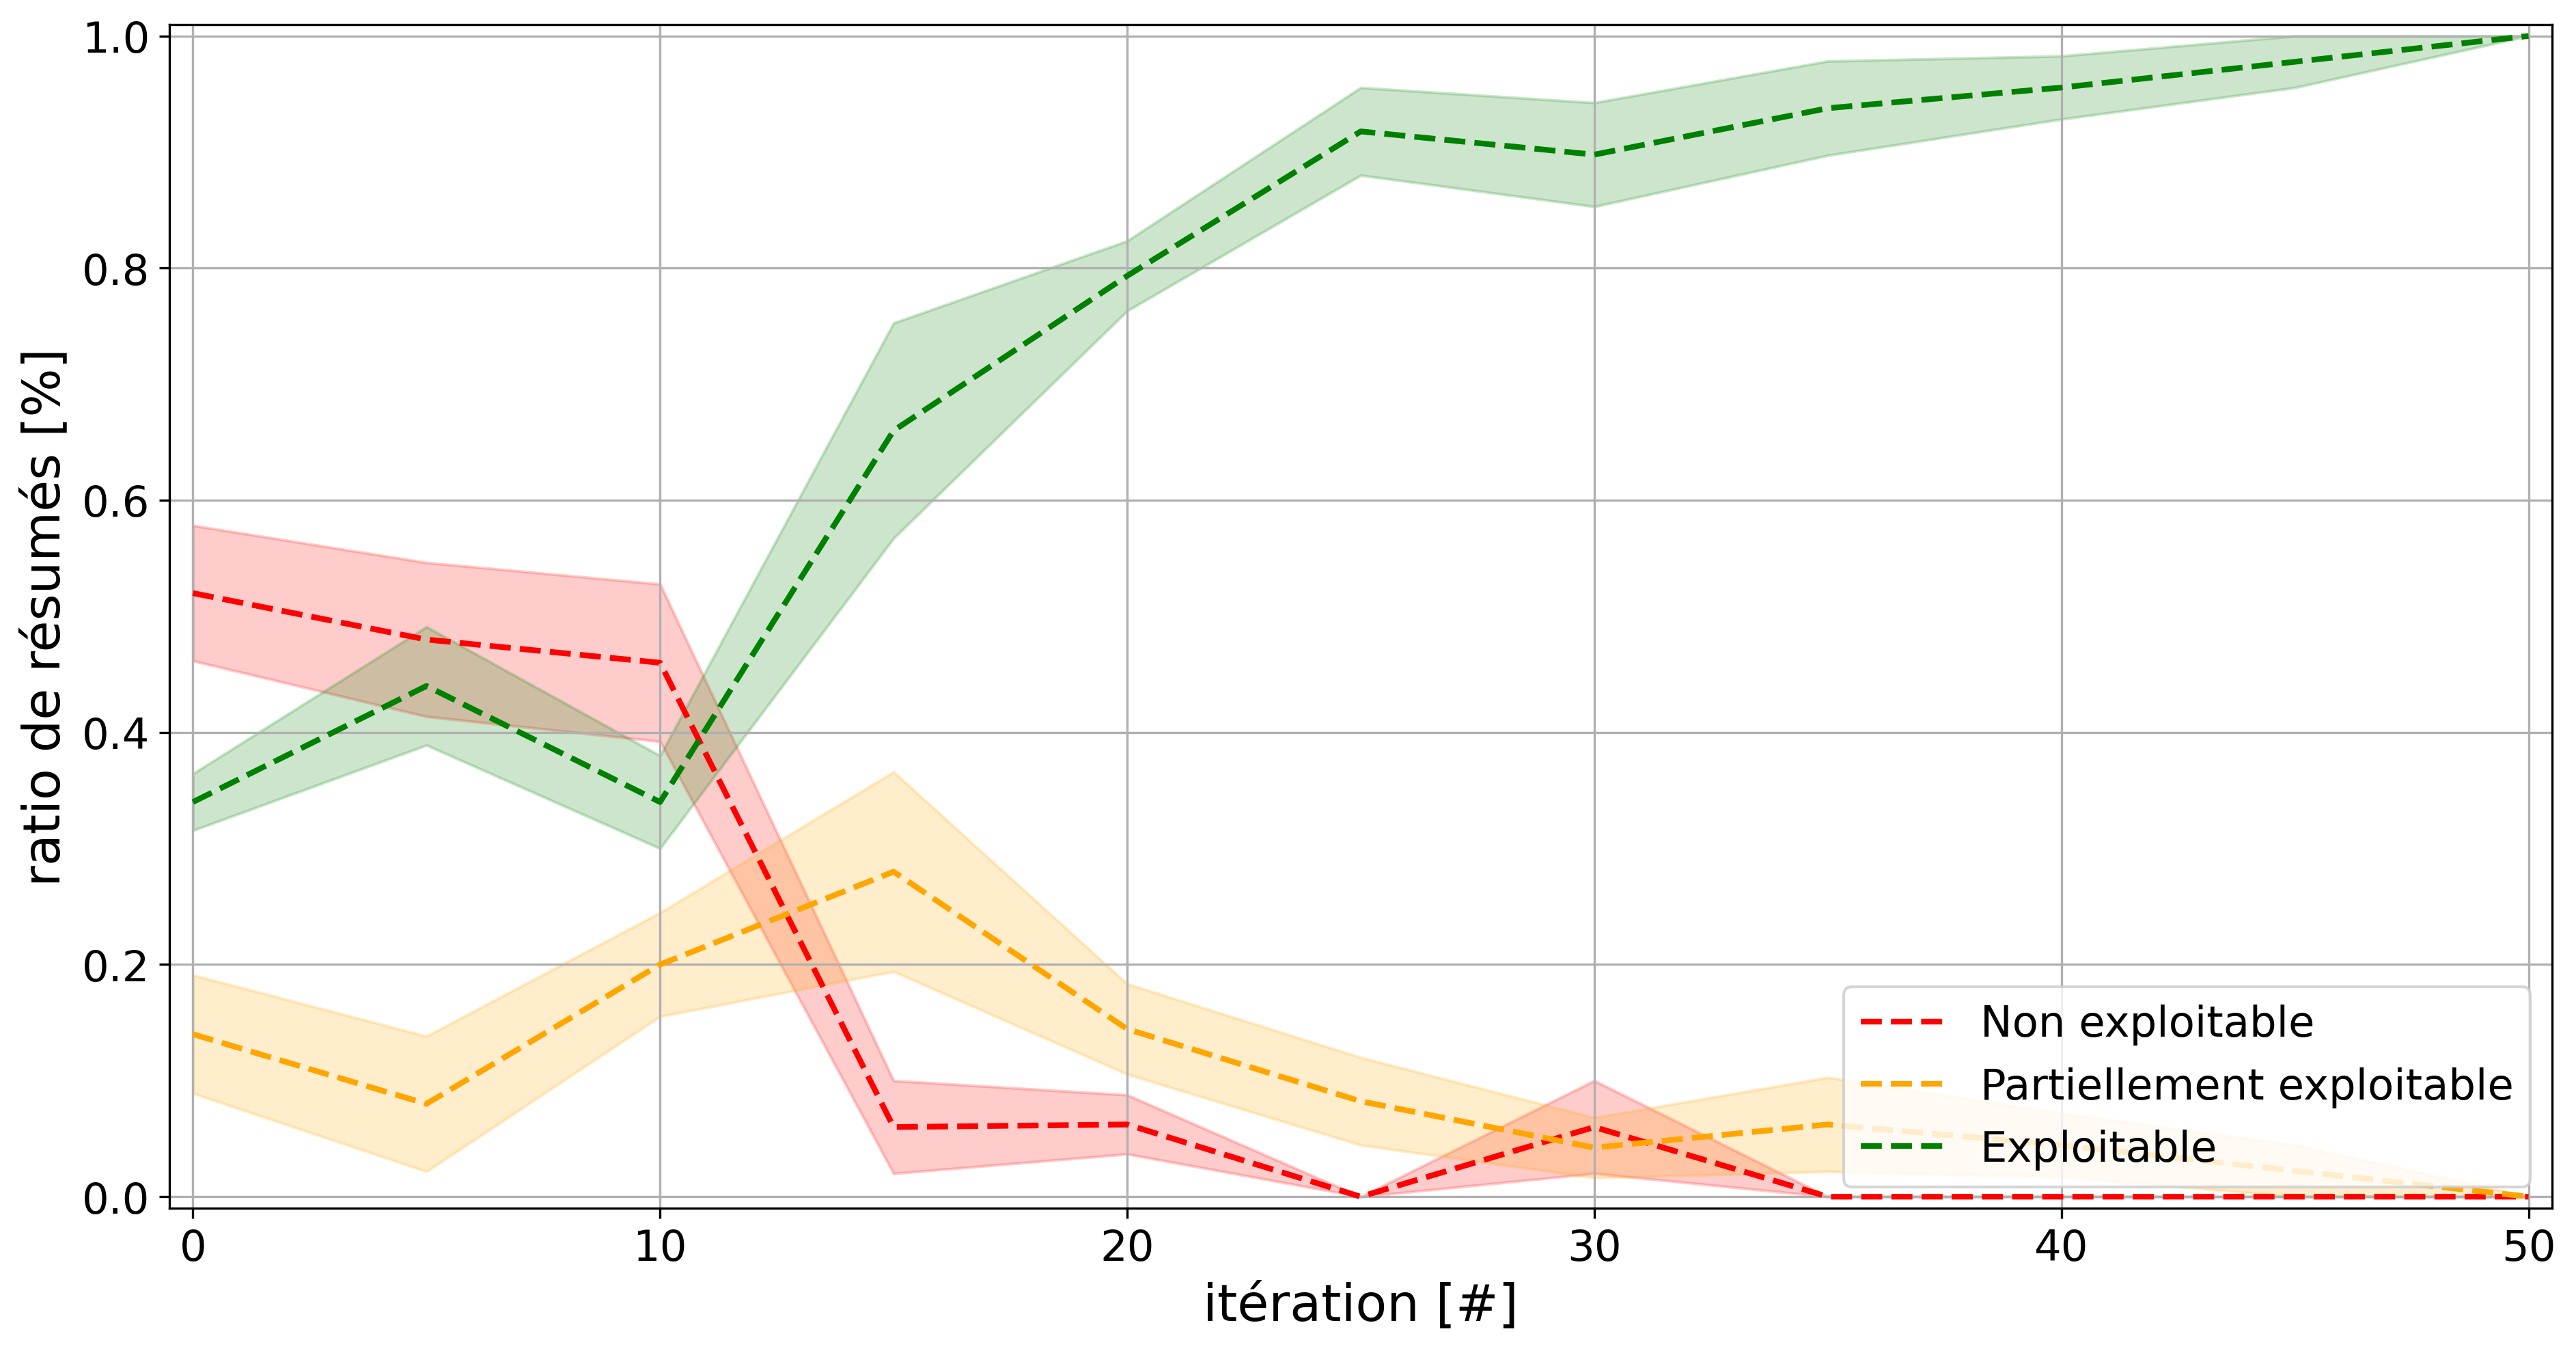
\includegraphics[width=0.95\textwidth]{figures/etude-pertinence-llm-check-resume-annotation-favori}
				\caption{Évolution de la pertinence métier moyenne en fonction du nombre d'itérations de la méthode.
				Cette pertinence, exprimée en proportion du nombre de \textit{clusters}, est estimée sur la base du résumé automatique des \textit{clusters} par un modèle de langue et est retranscrite en trois niveaux : \texttt{exploitable} en vert, \texttt{partiellement exploitable} en orange, et \texttt{non exploitable} en rouge.}
				\label{figure:4.4.3-ETUDE-PERTINENCE-RESUME-AUTOMATIQUE}
			\end{figure}
			
			% Description de deux cas d'études.
			Pour aller plus loin, reprenons les \textit{clusters} que nous avons utilisé comme cas d'étude lors de l'analyse linguistique à l'aide de la maximisation des traits (cf. \textsc{Section~\ref{section:4.4.2-ETUDE-PERTINENCE-PATTERNS-LINGUISTIQUES}}).
			
			% Exemple d'un cluster qui est bien formé dès le début.
			D'abord, reprenons l'exemple de l'évolution d'un \textit{cluster} bien formé dès l'itération $0$, précédemment détaillé dans la \textsc{Table~\ref{table:4.4.2-ETUDE-PERTINENCE-PATTERNS-LINGUISTIQUES-GESTION-SANS-CONTACT}} et dont les résumés automatiques sont présentés dans la \textsc{Table~\ref{table:4.4.3-ETUDE-PERTINENCE-RESUME-AUTOMATIQUE-GESTION-SANS-CONTACT}}.
			Nous constatons effectivement que les synthèses générées par le modèle identifie sans ambiguïté le thème du paiement sans contact, même si le résumé de l'itération $0$ énumère longuement les actions réalisables sur ce sujet.
			
			\todo[inline]{A REDIGER: tableau avec exemples ?}
			
			\begin{table}[!htb]
				\begin{center}
				\def\arraystretch{0.8}  % interligne
				\begin{tabular}{|c|c|}
				
				\hline
				% ENTETE DU TABLEAU
				Identification
					& \multirow{2}{*}{
						Résumé automatique du cluster (\texttt{LLM})
					}
					\tabularnewline
				du cluster
					&
					\tabularnewline
					\hline
				
				% Exemple 1.1:
				{ \footnotesize Tentative: $1$ }
					& \multirow{5}{*}{\parbox{12cm}{
						\footnotesize La thématique traitée dans ces textes est la gestion de l'activation, la désactivation, la modification ou la nécessité d'utiliser le paiement sans contact ou le NFC (Near Field Communication) sur les cartes de paiement bancaires.
					}}
					\tabularnewline
				{ \footnotesize Itération: $0$ }
					&
					\tabularnewline
				{ \footnotesize Cluster: $0$ }
					&
					\tabularnewline
				{ \footnotesize Avis initial: }
					&
					\tabularnewline
				{ \footnotesize \color{colorDarkPastelGreen} \texttt{Exploitable} }
					&
					\tabularnewline
					\hline
					
				% Exemple 1.2:
				{ \footnotesize Tentative: $1$ }
					& \multirow{5}{*}{\parbox{12cm}{
						\footnotesize Les textes traitent de la gestion et de l'utilisation du paiement sans contact (NFC) sur les cartes bancaires.
					}}
					\tabularnewline
				{ \footnotesize Itération: $15$ }
					&
					\tabularnewline
				{ \footnotesize Cluster: $0$ }
					& 
					\tabularnewline
				{ \footnotesize Avis initial: }
					&
					\tabularnewline
				{ \footnotesize \color{colorDarkPastelGreen} \texttt{Exploitable} }
					&
					\tabularnewline
					\hline
					
				\end{tabular}
				\end{center}
				\caption{Extrait de de l'analyse de résumés automatiques de \textit{clusters} exploitables dès la première itération.
				Ces \textit{clusters} représentent la thématique \texttt{gestion\_sans\_contact} entre l'itération $0$ (initialisation) et l'itération $15$ (atteinte de la vérité terrain).
				La seconde colonne expose le résumé obtenu en appelant un large modèle de langage (\texttt{gpt-3.5-turbo}) sur une tâche de résumé.
				}
				\label{table:4.4.3-ETUDE-PERTINENCE-RESUME-AUTOMATIQUE-GESTION-SANS-CONTACT}
			\end{table}
			
			% Exemple d'un cluster qui se forme.
			Ensuite, intéressons nous l'exemple de l'évolution des \textit{clusters} en cours de formations détaillés dans la \textsc{Table~\ref{table:4.4.2-ETUDE-PERTINENCE-PATTERNS-LINGUISTIQUES-GESTION-SANS-CONTACT}} et dont les résumés automatiques sont présentés dans la \textsc{Table~\ref{table:4.4.3-ETUDE-PERTINENCE-RESUME-AUTOMATIQUE-GESTION-SANS-CONTACT}}.
			À l'itération $0$, le résumé proposé est une longue énumération de $9$ thématiques différentes sur la gestion de carte bancaires : puisque le jeu de données entier traite des cartes bancaires, nous identifions clairement ce \textit{cluster} comme non exploitable.
			À l'itération $10$, nous ne distinguons plus que deux sujets principaux : le déblocage de carte, et l'utilisation de numéros de cartes virtuelles, ce qui est en accord avec notre précédente analyse.
			À partir de l'itération $15$, ces deux thématiques se retrouvent bien séparées dans deux \textit{clusters} différents, et chacune est identifiable via le résumé proposé : on note toutefois que si la thématique principale est identifiée, alors l'énumération de détails est plutôt portée sur les actions réalisables avec cette thématique ("\textit{création}", "\textit{activation}", "\textit{suppression}" pour la classe \texttt{gestion\_carte\_virtuelle}).
			
			\begin{table}[!htb]
				\begin{center}
				\def\arraystretch{0.8}  % interligne
				\begin{tabular}{|c|c|}
				
				\hline
				% ENTETE DU TABLEAU
				Identification
					& \multirow{2}{*}{
						Résumé automatique du cluster (avec un \texttt{LLM})
					}
					\tabularnewline
				du cluster
					&
					\tabularnewline
					\hline

				% Exemple 2.1:
				{ \footnotesize Tentative: $1$ }
					& \multirow{5}{*}{\parbox{12cm}{
						\footnotesize La thématique des textes est la gestion des cartes bancaires, incluant la sécurité, les pertes, les vols, les blocages, les récupérations, le changement ou la commande de cartes, les garanties et assurances, les découverts, les paiements virtuels, les numéros virtuels et les plafonds de paiement autorisés.
					}}
					\tabularnewline
				{ \footnotesize Itération: $0$ }
					&
					\tabularnewline
				{ \footnotesize Cluster: $1$ }
					&
					\tabularnewline
				{ \footnotesize Avis initial: }
					&
					\tabularnewline
				{ \footnotesize \color{colorDarkPastelRed} \texttt{Non exploitable} }
					&
					\tabularnewline
					\hline
					
				% Exemple 2.2:
				{ \footnotesize Tentative: $1$ }
					& \multirow{6}{*}{\parbox{12cm}{
						\footnotesize Les textes traitent principalement de la gestion des cartes de paiement, de leur déblocage ou leur réactivation, et de l'utilisation de numéros de carte virtuelle pour les achats en ligne.
					}}
					\tabularnewline
				{ \footnotesize Itération: $10$ }
					&
					\tabularnewline
				{ \footnotesize Cluster: $2$ }
					&
					\tabularnewline
				{ \footnotesize Avis initial: }
					&
					\tabularnewline
				{ \footnotesize \color{colorCadmiumOrange} \texttt{Partiellement} }
					&
					\tabularnewline
				{ \footnotesize \color{colorCadmiumOrange} \texttt{exploitable} }
					&
					\tabularnewline
					\hline
					
				% Exemple 2.3a:
				{ \footnotesize Tentative: $1$ }
					& \multirow{5}{*}{\parbox{12cm}{
						\footnotesize Les textes concernent la gestion et l'utilisation des numéros de carte virtuelle pour les achats en ligne, notamment la création, l'activation, la suppression et la gestion de ces numéros virtuels.
					}}
					\tabularnewline
				{ \footnotesize Itération: $15$ }
					&
					\tabularnewline
				{ \footnotesize Cluster: $2$ }
					&
					\tabularnewline
				{ \footnotesize Avis initial: }
					&
					\tabularnewline
				{ \footnotesize \color{colorDarkPastelGreen} \texttt{Exploitable} }
					&
					\tabularnewline
					\hline
					
				% Exemple 2.3b:
				{ \footnotesize Tentative: $1$ }
					& \multirow{5}{*}{\parbox{12cm}{
						\footnotesize La thématique traitée dans ces textes est le déblocage, le déverrouillage ou la réactivation de cartes bancaires bloquées.
					}}
					\tabularnewline
				{ \footnotesize Itération: $15$ }
					&
					\tabularnewline
				{ \footnotesize Cluster: $4$ }
					&
					\tabularnewline
				{ \footnotesize Avis initial: }
					&
					\tabularnewline
				{ \footnotesize \color{colorDarkPastelGreen} \texttt{Exploitable} }
					&
					\tabularnewline
					\hline
					
				\end{tabular}
				\end{center}
				\caption{Extrait de de l'analyse de résumés automatiques de \textit{clusters} évoluant de non exploitables à exploitables.
				Ces \textit{clusters} représentent la conception des thématiques \texttt{gestion\_carte\_virtuelle} et \texttt{deblocage\_carte}, entre l'itération $0$ (initialisation) et l'itération $15$ (atteinte de la vérité terrain).
				La seconde colonne expose le résumé obtenu en appelant un large modèle de langage (\texttt{gpt-3.5-turbo}) sur une tâche de résumé.
				}
				\label{table:4.4.3-ETUDE-PERTINENCE-RESUME-AUTOMATIQUE-DEBLOCAGE-CARTE-GESTION-CARTE-VIRTUELLE}
			\end{table}
			
			% Présence de quelques cas abhérants.
			De manière plus globale, en considérant les $376$ \textit{clusters} évalués lors des itérations n'ayant pas encore atteint la vérité terrain\footnote{Nous n'incluons pas les itérations ayant atteint la vérité terrain car les \textit{clusters} sont alors stables et cohérents, donc le modèle n'a aucun obstacle pour générer un résumé sans ambiguïté ni hallucination.}, les résumés automatiques permettent d'identifier les mêmes thématiques qu'une vérification manuelle dans $85$\% des cas ($312$ \textit{clusters}).
			Concernant les $15$\% de différences, nous avons différents cas de figure :
			\begin{itemize}
				\item si le modèle génère un résumé concis, certaines thématiques peuvent être ignorées : 
				\item à l'inverse, les données aberrantes ou isolées d'un \textit{cluster} peuvent influencer le résumé, donnant l'illusion que plusieurs thématiques sont présentes alors qu'une seule ne l'est réellement ;
				\item le résumé issu du large modèle de langage peut aussi identifier des thématiques auquel l'expert n'aurait pas pensé : c'est le cas dans les \textit{clusters} $7$ et $8$ de la tentative $1$ à l'itération $0$, où les thématiques \texttt{gestion\_carte\_mastercard} et \texttt{gestion\_carte\_visa} sont proposées dans la synthèse, mais n'aurait pas été par un expert (il n'y a pas de différences aussi significatives entre les deux réseaux de cartes bancaires pour justifier une gestion séparée) ;
				\item enfin, le modèle peut aussi générer des hallucinations n'ayant rien à voir avec les données en entrée : c'est le cas avec le cluster $9$ de la tentative $2$ à l'itération $10$, où le cluster est composé de $2$ questions (« \textit{Comment obtenir une Mastercard ?} » et « \textit{Désactiver les numéros virtuels.} ») et où le résumé parle de "\textit{sécurisation des transactions bancaires}"
			\end{itemize}

		%%% Discussion
		\subsubsection{Discussion}
			\todo[inline]{A REDIGER}
		
			% Remaques expérience utilisateur.
			\todo[inline]{A REDIGER: C'est super pratique, super accessible}
			\todo[inline]{A REDIGER: C'est parfois un peu ambigu...}
			
			% Conclusions et suggestion.
	
	
	%%%
	%%% Subsection 4.4.4: Étude de la cohérence statistique de la base d'apprentissage en cours de construction
	%%%
	%\subsection{Étude de la cohérence statistique de la base d'apprentissage en cours de construction}
	%\label{section:4.4.4-ETUDE-PERTINENCE-COHERENCE}
	%	
	%	% Objectif de l'expérience.
	%	\todo[inline]{A REDIGER: objectif de l'expérience}
	%
	%	%%% Protocole expérimental.
	%	\subsubsection{Protocole expérimental}
	%		\todo[inline]{A REDIGER}
	%		% Axiome.
	%		% Pseudo-code.
	%		% Détails de l'expérience.
	%		% Référence scripts.
	%
	%	%%% Résultats
	%	\subsubsection{Résultats obtenus}
	%		\todo[inline]{A REDIGER}
	%	
	%		% Description statistiques.
	%		
	%		% Exemple.
	%		
	%		% Figure.
	%		%
	%		\begin{figure}[!htb]
	%			\centering
	%			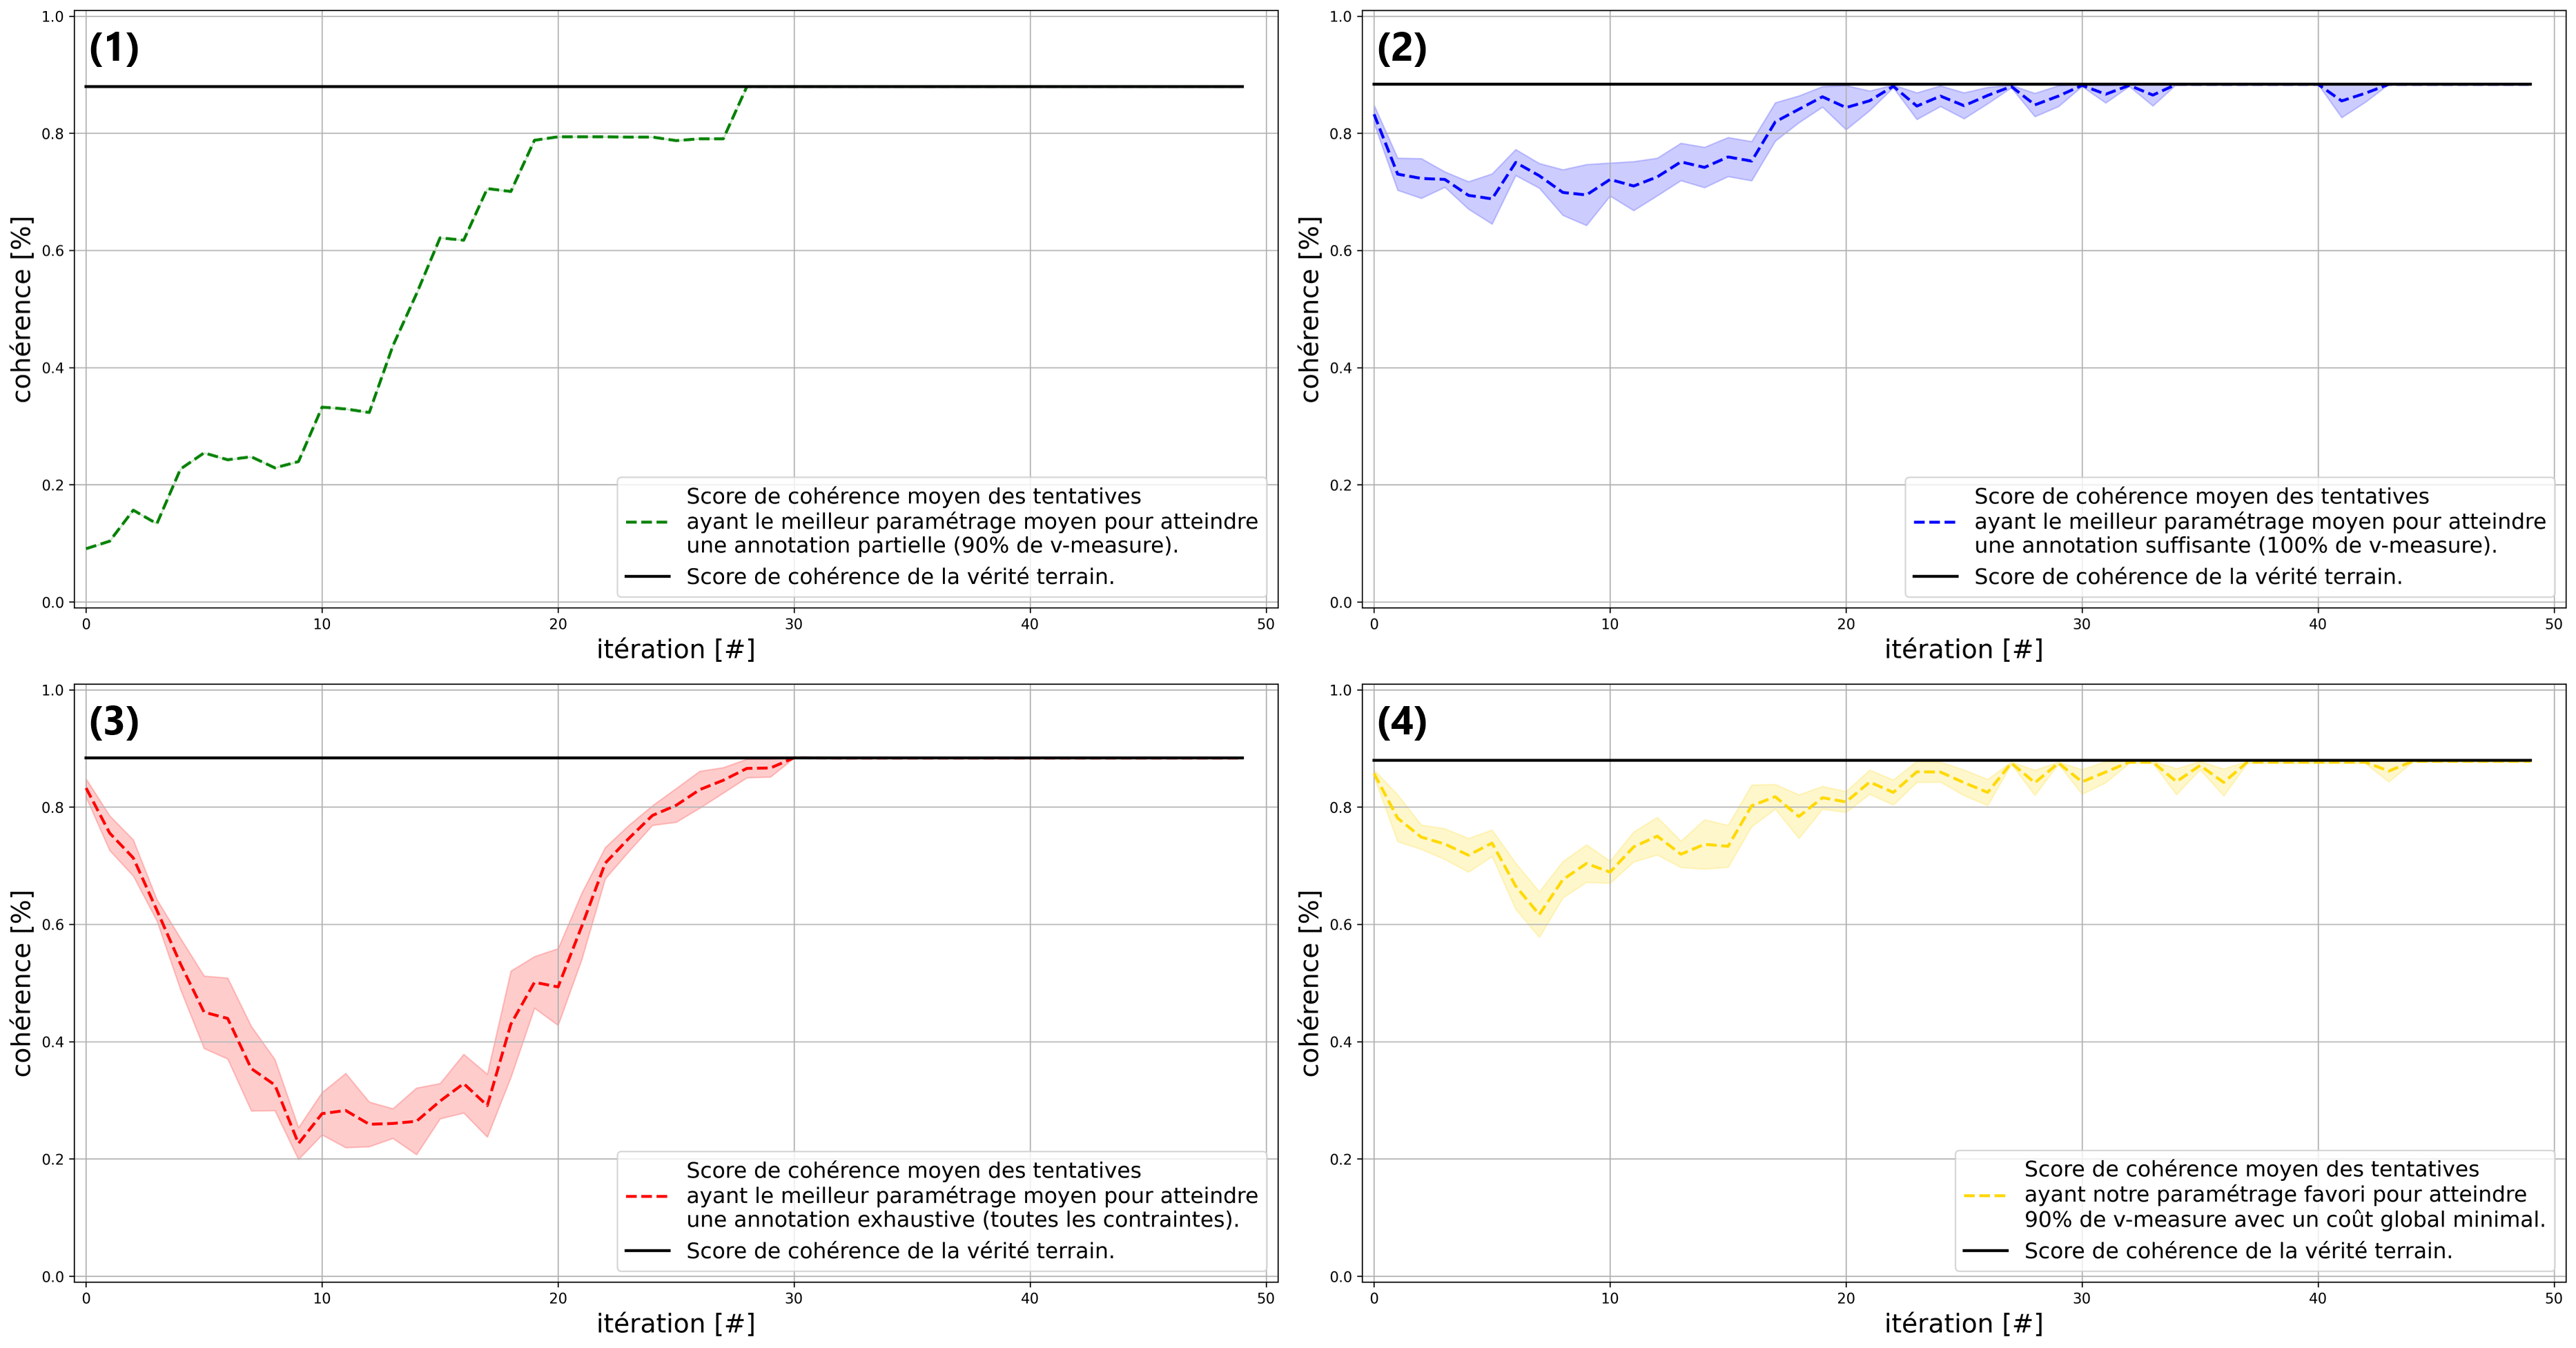
\includegraphics[width=0.95\textwidth]{figures/etude-pertinence-consistence}
	%			\caption{Évolution du score de cohérence moyen des tentatives en fonction de leur paramétrage : \textbf{(1)} meilleur paramétrage moyen une annotation partielle (\texttt{90}\% de \texttt{v-measure}), \textbf{(2)} meilleur paramétrage moyen une annotation suffisante (\texttt{100}\% de \texttt{v-measure}), \textbf{(3)} meilleur paramétrage moyen une annotation exhaustive (annoter toutes les contraintes possibles), et \textbf{(4)} paramétrage favori (\texttt{90}\% de \texttt{v-measure} avec un coût minimal). \\
	%			Note : \textit{Le score de cohérence de la vérité terrain peut varier en fonction des méthodes de prétraitements et de vectorisation utilisées.}}
	%			\label{figure:4.4.4-ETUDE-PERTINENCE-COHERENCE-ANNOTATION}
	%		\end{figure}
	%
	%	%%% Discussion
	%	\subsubsection{Discussion}
	%		\todo[inline]{A REDIGER}
	%	
	%		% Remaques expérience utilisateur.
	%		
	%		% Conclusions et suggestion.
	
	
	%%%%%--------------------------------------------------------------------
	%%%%% Section 4.5: Hypothèse de rentabilité.
	%%%%%--------------------------------------------------------------------
	\newpage
	\section{Évaluation de l'hypothèse de rentabilité}
\label{section:4.5-HYPOTHESE-RENTABILITE}

	%%%
	%%% Introduction / Transition.
	%%%
	Dans les études précédentes, le cas d'arrêt de notre méthodologie d'annotation basée sur le \texttt{Clustering Interactif} était conditionné à la vérité terrain.
	En effet, nous utilisions un seuil de $90$\% de \texttt{v-measure}, caractérisant une annotation dite "partielle" de la base d'apprentissage.
	Cependant, une telle référence n'est pas accessible en situation réelle car l'objectif de notre méthode est précisément de construire cette vérité terrain.
	Nous devons donc nous intéresser à d'autres moyens pour estimer la rentabilité d'une itération supplémentaire, et pouvoir ainsi définir de nouveaux cas d'arrêt pour le \texttt{Clustering Interactif}.
	Pour cela, nous aimerions vérifier l'hypothèse suivante :
	
	%%%
	%%% Formulation des hypothèses.
	%%%
	\begin{tcolorbox}[
		title=\faVial~\textbf{Hypothèse de rentabilité}~\faVial,
		colback=colorTcolorboxHypothesis!15,
		colframe=colorTcolorboxHypothesis!75,
		width=\linewidth
	]
		\textguillemets{\textbf{
			Au cours d'une méthodologie d'annotation basée sur le \texttt{Clustering Interactif}, il est possible d'estimer la rentabilité d'une itération supplémentaire de la méthode, et ainsi d'établir des cas d'arrêt indépendants d'une vérité terrain pour obtenir une base d'apprentissage satisfaisante.
		}} \\
		
		% Figure.
		La \textsc{Figure~\ref{figure:4.5-HYPOTHESE-RENTABILITE}} illustre cette hypothèse et la perspective de pouvoir estimer le rapport entre le gain de pertinence obtenu et le coût nécessaire pour l'obtenir.
		%
		\begin{figure}[H]  % keep [H] to be in the tcolorbox.
			\centering
			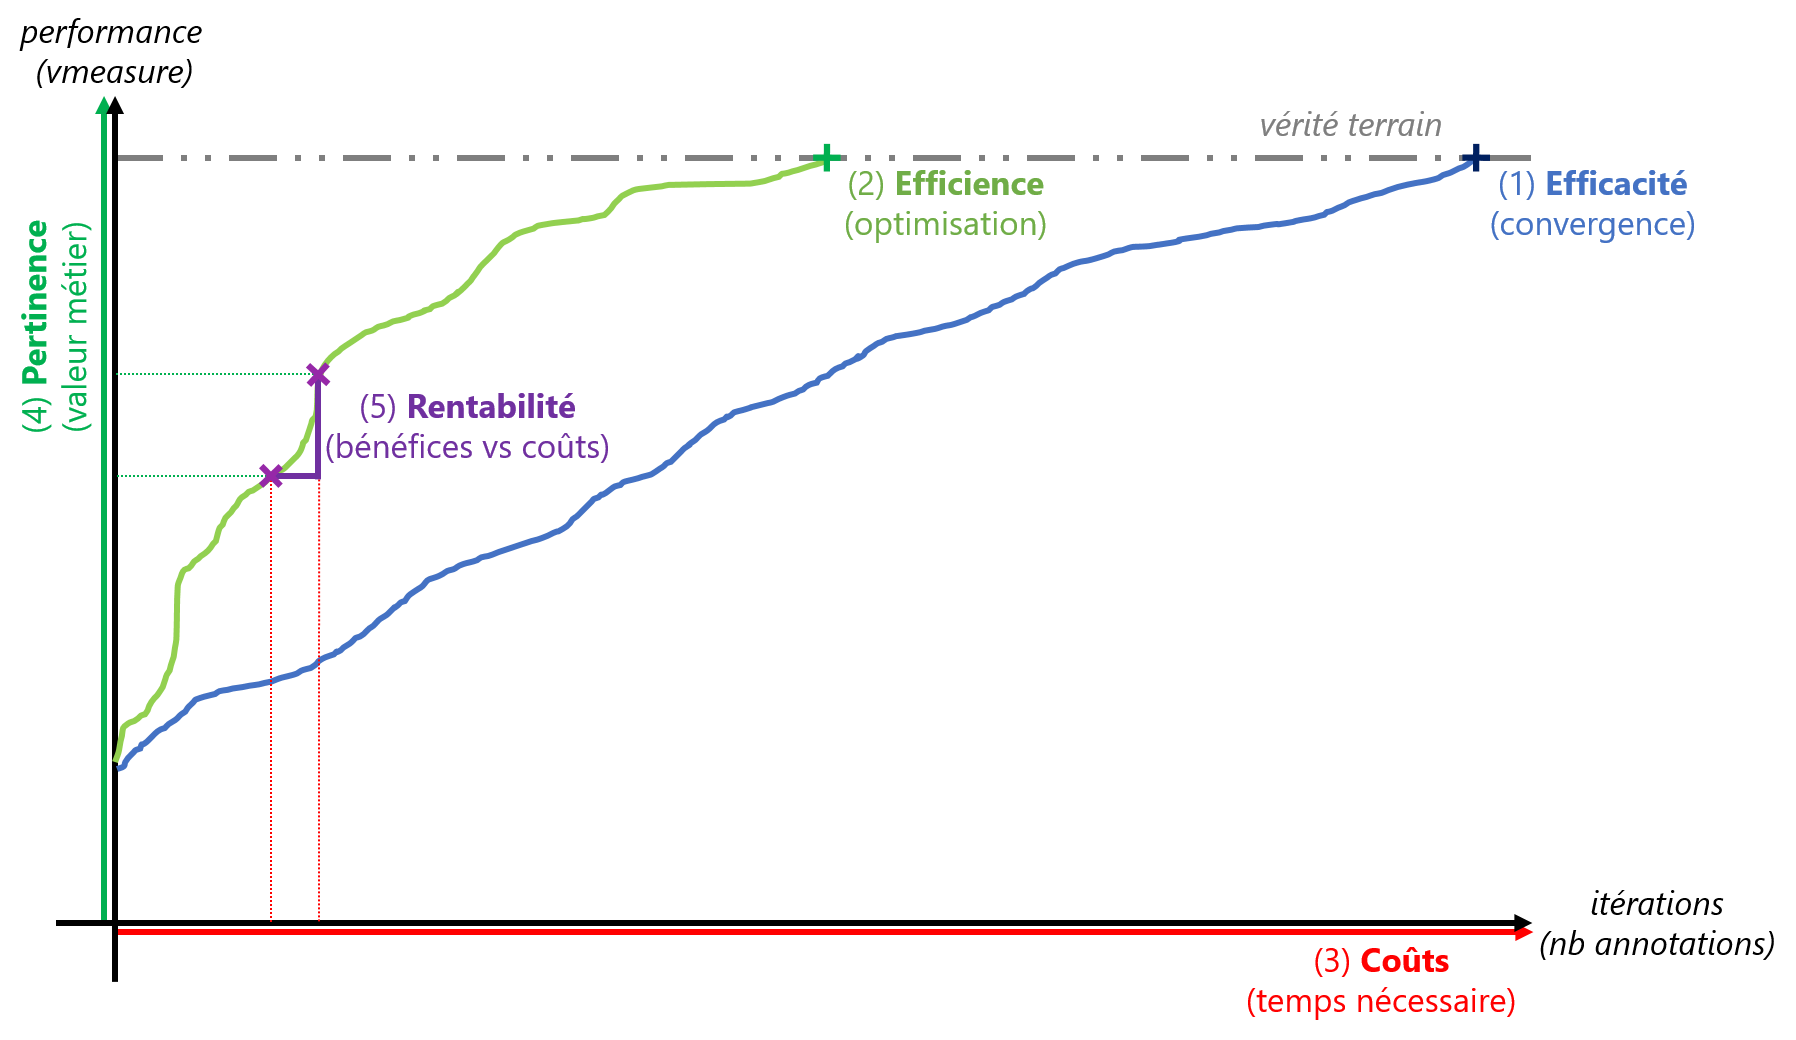
\includegraphics[width=0.95\textwidth]{figures/hypotheses-05-rentabilite}
			\caption{
				Illustration des études réalisées sur le \texttt{Clustering Interactif} (\textit{étape 5/6}) en schématisant l'évolution de la \textbf{pertinence} (\textit{valeur métier évaluée par l'expert, exprimée en nombre de clusters}) d'une base d'apprentissage en cours de construction, en fonction du coût temporel de la méthode (\textit{temps nécessaire à l'expert métier et à la machine}), ainsi que la \textbf{rentabilité} de chaque itération de la méthode (\textit{rapport entre le gain potentiel de pertinence et le coût à investir}).
			}
			\label{figure:4.5-HYPOTHESE-RENTABILITE}
		\end{figure}
	\end{tcolorbox}
		
	% Résumé des études.
	Afin de vérifier cette hypothèse, nous explorons deux approches :
	\begin{itemize}
		\item l'évolution de l'\textbf{accord entre l'annotation de l'expert et le \textit{clustering}} sur lequel est basé l'échantillon d'annotation, permettant d'estimer si la machine doit encore être corrigée par l'annotateur  (cf. \textsc{Section~\ref{section:4.5.1-ETUDE-RENTABILITE-ACCORD-ANNOTATION-CLUSTERING}}) ; et
		\item l'évolution de la \textbf{différence entre deux \textit{clustering} successifs}, permettant de mesurer s'il y a eu des changements visibles dans le partitionnement des données après l'ajout des dernières contraintes (cf. \textsc{Section~\ref{section:4.5.2-ETUDE-RENTABILITE-SIMILARITE-CLUSTERING}}).
	\end{itemize}
	
	
	%%%
	%%% Subsection 4.5.1: Étude de l'évolution d'accord entre l'annotation et le \textit{clustering}.
	%%%
	\subsection{Étude de l'évolution d'accord entre l'annotation et le \textit{clustering}}
	\label{section:4.5.1-ETUDE-RENTABILITE-ACCORD-ANNOTATION-CLUSTERING}
		
		% Objectif de l'expérience.
		Nous cherchons à trouver un cas d'arrêt du \texttt{Clustering Interactif} ne nécessitant pas de comparaison avec une vérité terrain, et notre première intuition concerne l'étude des annotations réalisées.
		En effet, à chaque itération, l'expert annote un échantillon de contraintes dans le but de confirmer ou de corriger le \textit{clustering} de l'itération précédente.
		Or, après un nombre suffisant d'itérations, le \textit{clustering} commence à se stabiliser : il devrait donc y avoir davantage d'annotations qui confirment le \textit{clustering} que d'annotations qui le corrigent, puis n'avoir que des accords entre les annotations et le \textit{clustering}.
		Ainsi, nous allons étudier l'évolution du nombre de contraintes annotées qui approuvent le partitionnement des données obtenu, et essayer d'adapter cette analyse en cas d'arrêt pour notre méthode d'annotation.
	
		%%% Protocole expérimental.
		\subsubsection{Protocole expérimental}
			
			% Axiome.
			\begin{leftBarWarning}
				Dans le cadre de cette étude, nous supposons que l'expert métier connaît parfaitement le domaine traité dans ce jeu de données, et qu'il est capable de caractériser sans ambiguïté la similitude entre deux données issues de cet ensemble.
			\end{leftBarWarning}
			
			% Pseudo-code.
			Pour résumer le protocole expérimental que nous détaillons ci-dessous, une description en pseudo-code est disponible dans l'\textsc{Algorithme~\ref{algorithm:4.5.1-ETUDE-RENTABILITE-ACCORD-ANNOTATION-CLUSTERING-PROTOCOLE}}.
			
			\begin{algorithm}
				\KwData{jeux de données annotées (vérités terrains)}
				%
				\ForEach{jeu de données à tester}{
					\textbf{initialisation (données)}: récupérer les données et la vérité terrain \;
					\textbf{initialisation (contraintes)}: créer une liste vide de contraintes \;
					\textbf{prétraitements}: supprimer le bruit dans les données avec \texttt{prep.simple} \;
					\textbf{vectorisation}: transformer les données en vecteurs avec \texttt{vect.tfidf} \;
					\textbf{clustering initial}: regrouper les données par similarité avec \texttt{clust.kmeans.cop} \;
					\Repeat{annotation de toutes les contraintes possibles}{
						\textbf{échantillonnage}: sélectionner des contraintes avec \texttt{samp.closest.diff} \;
						\textbf{simulation d'annotation}: déterminer les contraintes avec la vérité terrain \;
						\textbf{intégration}: ajouter les nouvelles contraintes au gestionnaire de contraintes \;
						\textbf{rentabilité}: calculer l'accord entre l'annotation et le \textit{clustering} précédent \;
						\textbf{clustering}: regrouper les données par similarité avec \texttt{clust.kmeans.cop} \;
					}
				}
				\textbf{analyse 1}: afficher l'évolution de l'accord entre annotation et \textit{clustering} \;
				\textbf{analyse 2}: calculer la corrélation entre le score d'accord et le score de performance \;
				%
				\KwResult{discussion sur la rentabilité d'après l'accord entre annotation et \textit{clustering}}
				%
				\caption{\textit{
					Description en pseudo-code du protocole expérimental de l'étude de l'évolution d'accord entre l'annotation et le \textit{clustering}.
				}}
				\label{algorithm:4.5.1-ETUDE-RENTABILITE-ACCORD-ANNOTATION-CLUSTERING-PROTOCOLE}
			\end{algorithm}
			
			% Description de la vérité terrain.
			Nous utilisons comme vérité terrain le jeu de données \texttt{Bank Cards (v1.0.0)} : ce dernier traite des demandes les plus fréquentes des clients en ce qui concerne la gestion de leur carte bancaire.
			Il est composé de $500$ questions rédigées en français et réparties en $10$ classes (\texttt{perte ou vol de carte}, \texttt{carte avalée}, \texttt{commande de carte}, ...).
			Pour plus de détails, consulter l'\textsc{Annexe~\ref{annex:A.1-DATASET-BANK-CARDS}}.
			
			% Description des tentatives de la méthode et du calcul de rentabilité.
			Sur ce jeu de données, nous exécutons une tentative complète \footnote{
				Tentative complète : itérations d'échantillonnage, d'annotation et de \textit{clustering} jusqu'à annotation de toutes les contraintes possibles.
			}
			de la méthode du \texttt{Clustering Interactif} en utilisant notre paramétrage favori \footnote{
				Paramétrage favori (atteindre $90$\% de \texttt{v-measure} avec un coût minimal): prétraitements simples (\texttt{prep.simple}), vectorisation \texttt{TF-IDF} (\texttt{vect.tfidf}), \textit{clustering} \texttt{KMeans} avec modèle \texttt{COP} (\texttt{clust.kmeans.cop}) et échantillonnage des données les plus proches dans des \textit{clusters} différents (\texttt{sampl.closest.diff}).
			} (voir \textsc{Section~\ref{section:4.3-HYPOTHESE-COUTS}}), et cette tentative est répétée $5$ fois pour contrer les aléas statistiques des exécutions.
			À chaque itération, un lot de $50$ contraintes est sélectionné puis annotés en simulant l'action d'un expert métier, et nous évaluons l'accord entre ces nouvelles annotations et la proposition de partitionnement des données, partitionnement réalisé par le \textit{clustering} à l'itération précédente :
			\begin{itemize}
				\item il y a \textbf{accord} lorsqu'une contrainte de deux données issues d'un même \textit{cluster} est annotée \texttt{MUST-LINK}, ou lorsqu'une contrainte de deux données issues de deux \textit{clusters} différents est annotée \texttt{CANNOT-LINK} (cf. \textsc{Figure~\ref{figure:4.5.1-ETUDE-RENTABILITE-ACCORD-ANNOTATION-CLUSTERING-EXEMPLE} (1)}) ;
				\item il y a \textbf{désaccord} lorsqu'une contrainte de deux données issues d'un même \textit{cluster} est annotée \texttt{CANNOT-LINK}, ou lorsqu'une contrainte de deux données issues de deux \textit{clusters} différents est annotée \texttt{MUST-LINK} (cf. \textsc{Figure~\ref{figure:4.5.1-ETUDE-RENTABILITE-ACCORD-ANNOTATION-CLUSTERING-EXEMPLE} (2)}).
			\end{itemize}
			Nous pouvons ainsi calculer un score d'accord défini par le ratio entre le nombre d'accords et le nombre de contraintes annotées.
			Pour nous permettre de discuter de l'utilité de ce score pour prédire la stabilisation du \textit{clustering} et ainsi définir un cas d'arrêt de notre méthodologie d'annotation, nous calculons aussi le score de corrélation entre cet accord et la performance obtenue à l'aide d'une vérité terrain (la corrélation \texttt{r} de \textit{Pearson} (\cite{kirch:2008:pearson-correlation-coefficient}) est utilisée).

			\begin{figure}[!htb]
				\centering
				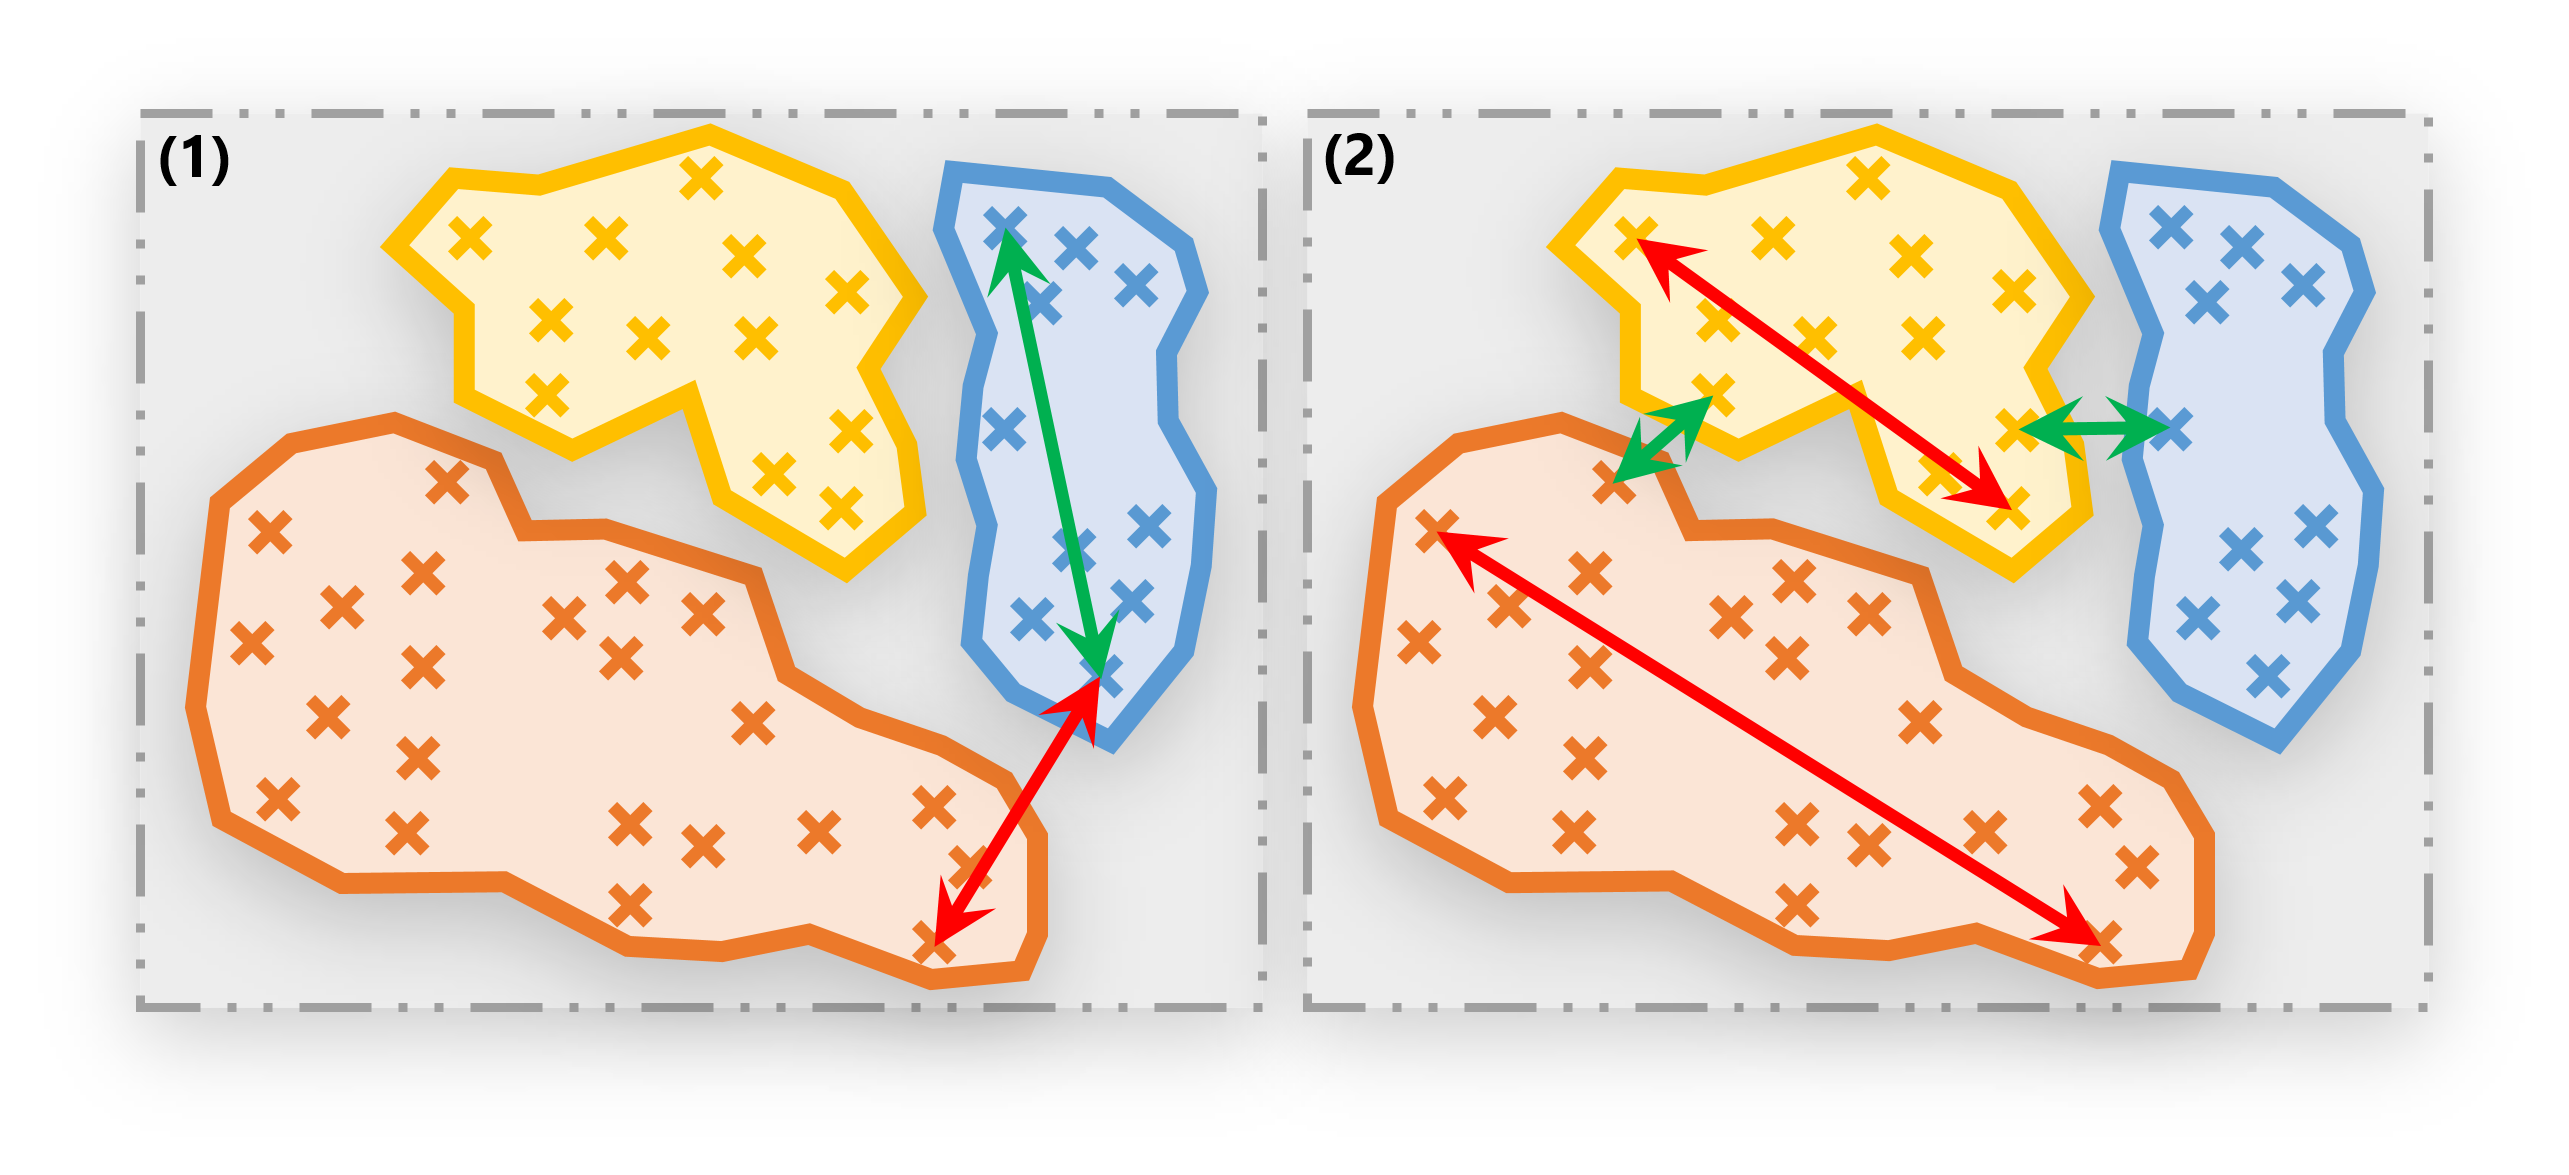
\includegraphics[width=0.70\textwidth]{figures/example-accord-annotation-clustering}
				\caption{
					Exemples d'accords et de désaccords entre les annotations d'une itération et le résultat du \textit{clustering} de l'itération précédente.
					Des contraintes \texttt{MUST-LINK} (flèches vertes) et \texttt{CANNOT-LINK} (flèches rouges) sont représentées dans deux situations : \textbf{(1)} montre des cas d'accords (\texttt{MUST-LINK} dans un même \textit{cluster}, \texttt{CANNOT-LINK} entre deux \textit{clusters} différents), et \textbf{(2)} montre des cas de désaccords (\texttt{MUST-LINK} entre deux \textit{clusters} différents, \texttt{CANNOT-LINK} dans un même \textit{cluster}).
				}
				\label{figure:4.5.1-ETUDE-RENTABILITE-ACCORD-ANNOTATION-CLUSTERING-EXEMPLE}
			\end{figure}
			
			\begin{leftBarIdea}
				Nous concentrons l'étude sur notre paramétrage favori (voir \textsc{Section~\ref{section:4.4.3-ETUDE-PERTINENCE-RESUME-AUTOMATIQUE}}).
				Cependant, afin de compléter notre discussion avec d'autres points de comparaison, nous analysons aussi les autres paramétrages implémentés, notamment les meilleurs paramétrages moyens identifiés lors de l'hypothèse d'efficience (voir \textsc{Section~\ref{section:4.2-HYPOTHESE-EFFICIENCE}}).
			\end{leftBarIdea}
			
			% Référence scripts.
			\begin{leftBarInformation}
				Les scripts de l'expérience, réalisés avec des \textit{notebooks} \texttt{Python} (\cite{van-rossum-drake:2009:python-reference-manual}), sont disponibles dans un dossier dédié de \cite{schild:2021:cognitivefactory-interactiveclusteringcomparativestudy}.
				De plus, les jeux de données ainsi que les implémentations de notre \texttt{Clustering Interactif} sont détaillés respectivement en \textsc{Annexe~\ref{annex:A-ANNEXE-DATASET}} et en \textsc{Annexe~\ref{annex:C-ANNEXE-IMPLEMENTATIONS}}.
			\end{leftBarInformation}

		%%% Résultats
		\subsubsection{Résultats obtenus}
			
			% Figure : croissance générale.
			La \textsc{Figure~\ref{figure:4.5.1-ETUDE-RENTABILITE-ACCORD-ANNOTATION-CLUSTERING}} représente l'évolution moyenne du score d'accord entre annotation et \textit{clustering} pour les quatre paramétrages mis en avant lors de nos études.
			Nous pouvons constater une tendance générale à la croissance de ce score d'accord : pour le paramétrage favori \textbf{(4)}, l'accord est plutôt faible au début de la méthode (inférieur à $45$\% avant l'itération $15$), puis devient de plus en plus fort (dépassant les $60$\%) pour finalement atteindre les $100$\% vers l'itération $45$.
			\begin{figure}[!htb]
				\centering
				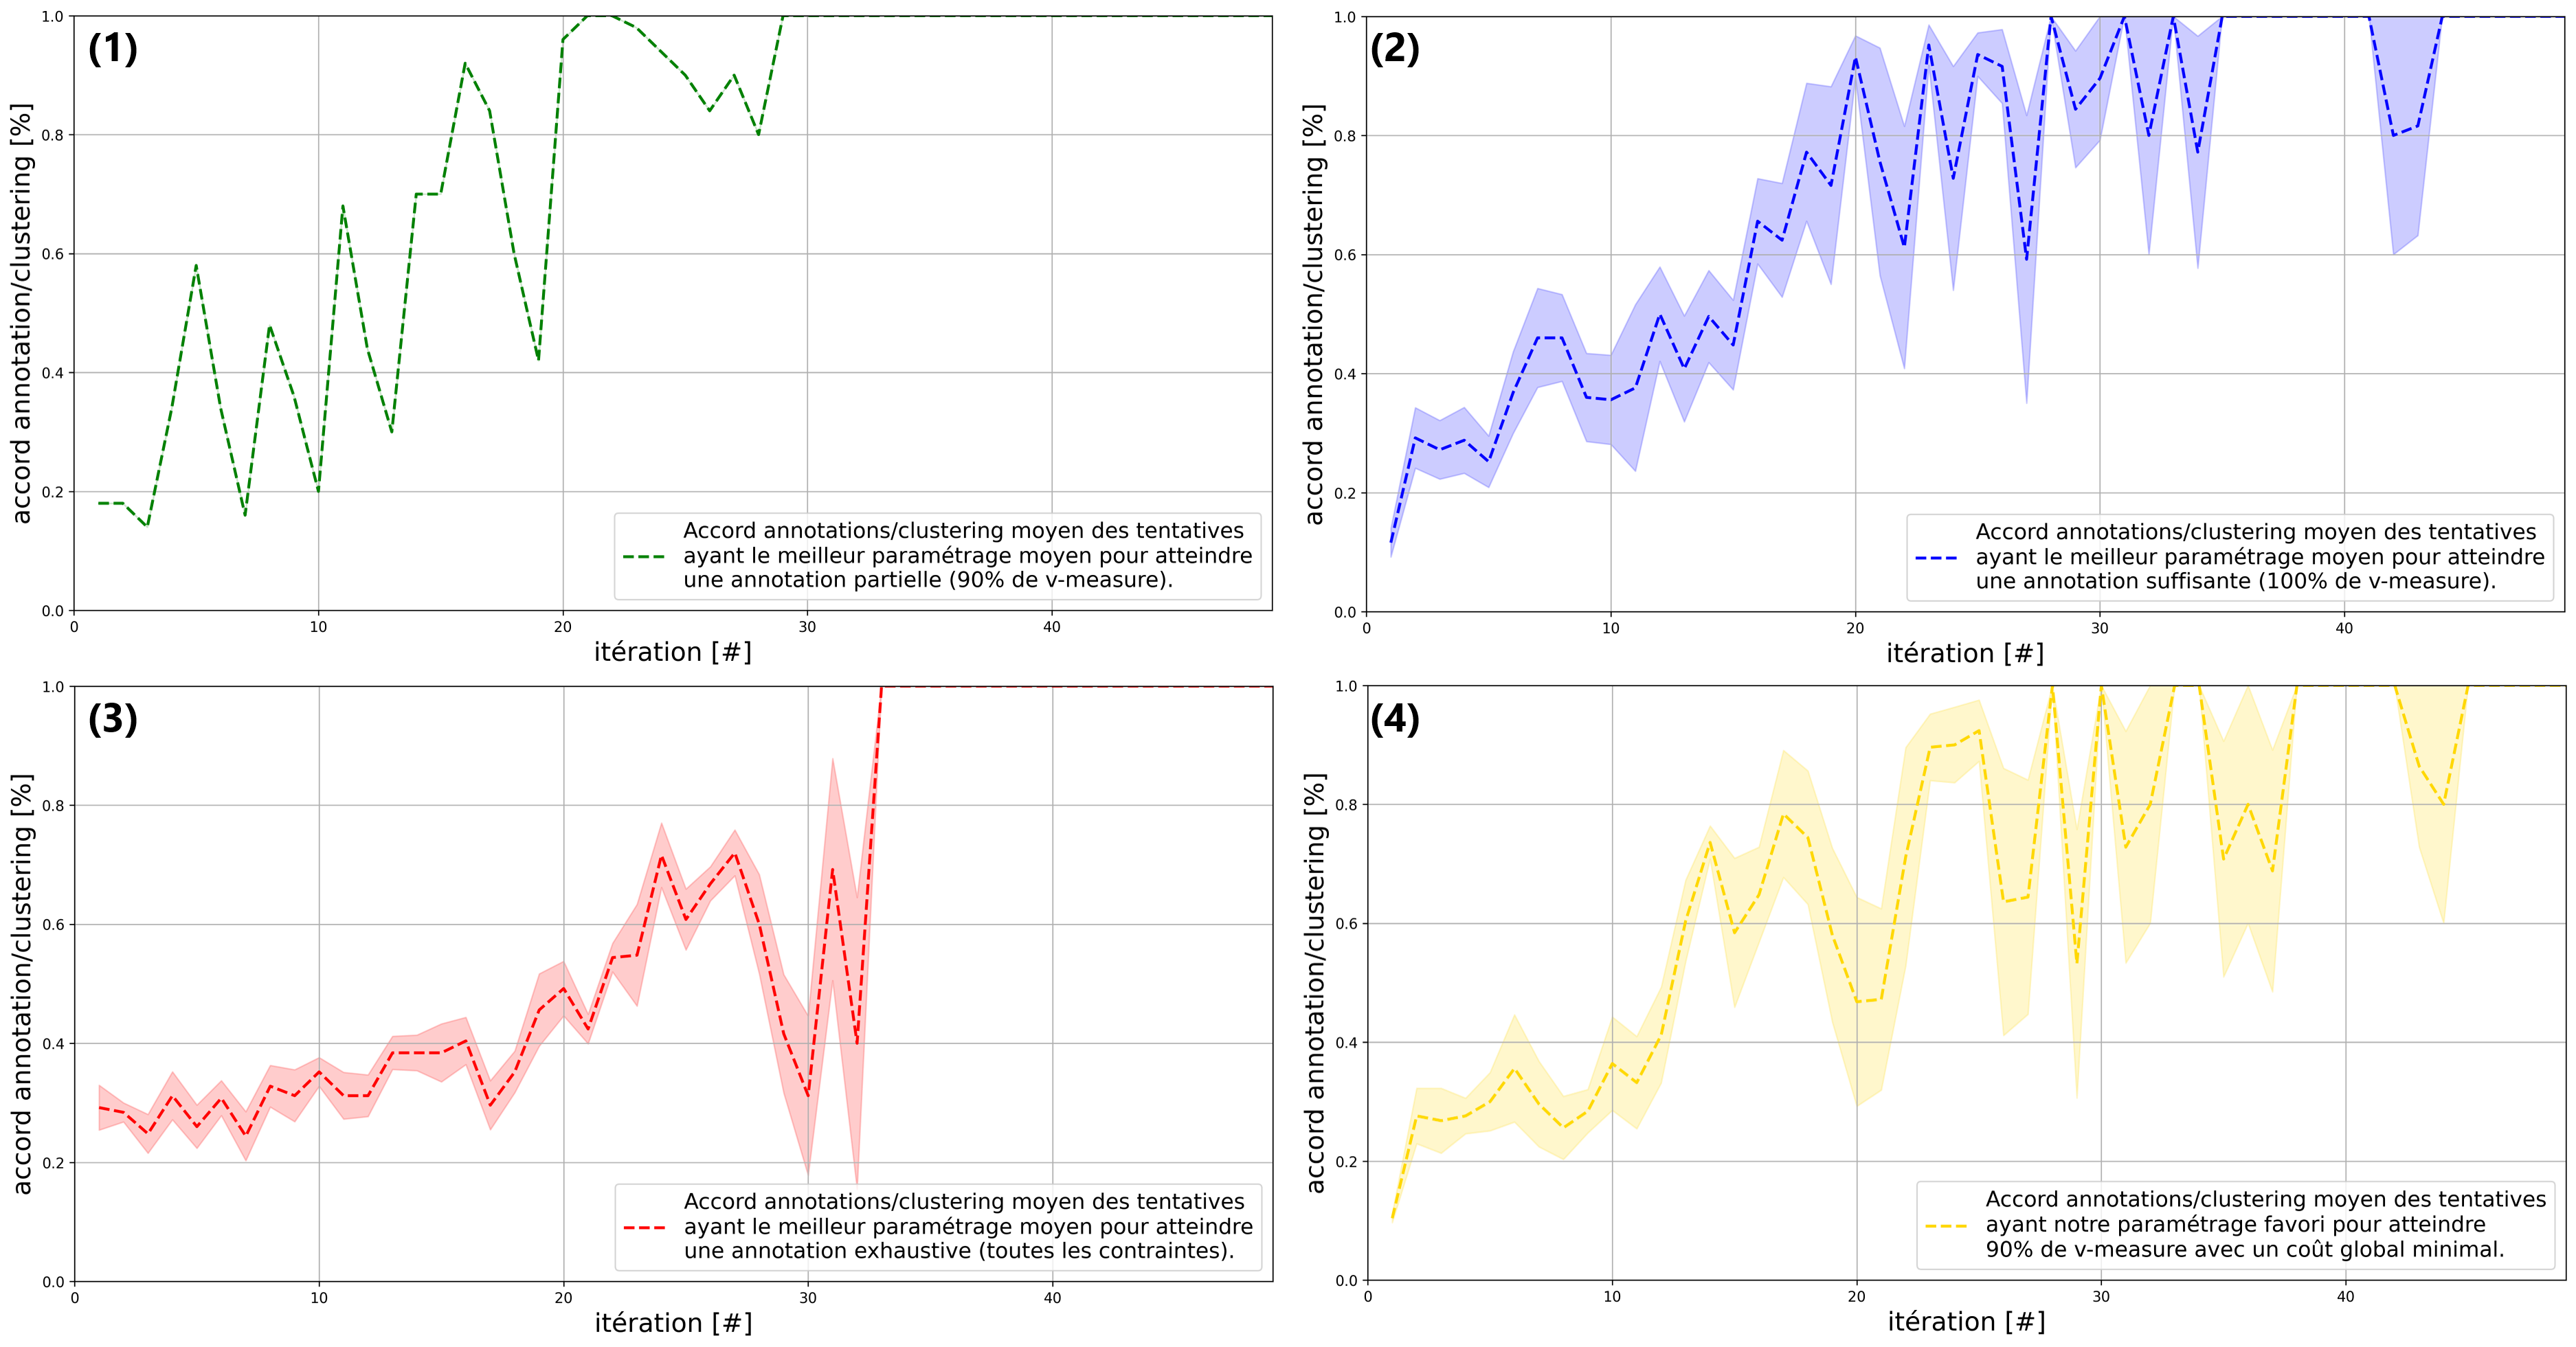
\includegraphics[width=0.95\textwidth]{figures/etude-rentabilite-accord-annotation}
				\caption{
					Évolution au cours des itérations de l'accord entre l'annotation de contraintes d'un expert et le résultat de \textit{clustering} sur lequel est basé l'échantillonnage de contraintes.
					Ces accords sont exprimés grâce à des lots de $50$ contraintes annotées.
					Les évolutions moyennes de différents paramétrages de la méthode sont exposées :
					\textbf{(1)} meilleur paramétrage moyen pour atteindre une annotation partielle ;
					\textbf{(2)} meilleur paramétrage moyen pour atteindre une annotation suffisante ;
					\textbf{(3)} meilleur paramétrage moyen pour atteindre une annotation exhaustive ;
					et \textbf{(4)} paramétrage favori.
					À titre d'information, les courbes en noir représentent l'évolution de la \texttt{v-measure} entre le \textit{clustering} et la vérité terrain.
				} 
				\label{figure:4.5.1-ETUDE-RENTABILITE-ACCORD-ANNOTATION-CLUSTERING}
			\end{figure}
			
			% Tableau : corrélation modérée.
			La \textsc{Table~\ref{table:4.5.1-ETUDE-RENTABILITE-CORRELATION-ACCORD-PERFORMANCE}} contient le score de corrélation entre cet accord et la performance théoriques obtenue grâce à la vérité terrain.
			Cette corrélation est modérée : $0.49$ sur l'ensemble des tentatives, $0.69$ sur les tentatives utilisant notre paramétrage favori.
			%
			\begin{table}[!htb]
				\begin{center}
				\begin{tabular}{|c|r|}
				
					\hline
					% ENTETE DU TABLEAU
					\rowcolor{colorTableHeader!15}
					\multicolumn{1}{|c|}{\shortstack[c]{
						Paramétrage
					}}
						& \multicolumn{1}{c|}{\shortstack[c]{
							Corrélation \texttt{r}
						}}
						\tabularnewline
						\hline \hline
					
					% Annotation partielle.
					Meilleur paramétrage moyen pour une annotation partielle \textbf{(1)}
						& $0.92$
						\tabularnewline
						\hline
					
					% Annotation suffisante.
					Meilleur paramétrage moyen pour une annotation suffisante \textbf{(2)}
						& $0.74$
						\tabularnewline
						\hline
					
					% Annotation exhaustive.
					Meilleur paramétrage moyen pour une annotation exhaustive \textbf{(3)}
						& $0.57$
						\tabularnewline
						\hline
					
					% Paramétrage favori
					Paramétrage favori \textbf{(4)}
						& $0.69$
						\tabularnewline
						\hline
					
					% Moyenne des $960$ tentatives.
					Moyenne des $960$ tentatives
						& $0.49$
						\tabularnewline
						\hline
					
				\end{tabular}
				\end{center}
				\caption{
					Score de corrélation \texttt{r} de \textit{Pearson} entre la performance du \textit{clustering} obtenu à l'aide d'une vérité terrain (\texttt{v-measure}) et le score d'accord entre annotation et \textit{clustering}.
				}
				\label{table:4.5.1-ETUDE-RENTABILITE-CORRELATION-ACCORD-PERFORMANCE}
			\end{table}
			
			% Description de la figure : croissance instable.
			Cependant, la tendance constatée est aussi saccadée par de nombreux pics pouvant faire perdre ou gagner jusqu'à $40$\% d'accord entre deux itérations.
			Des chutes d'accord peuvent intervenir au niveau des itérations où la similarité du \textit{clustering} avec la vérité terrain est pourtant forte, comme c'est le cas autour des itérations $29$ et $36$ où l'accord chute de plus de $25$\% alors que la \texttt{v-measure} avec la vérité terrain est constamment au dessus de de $95$\%.
			
			% Description de la figure : autres paramétrages
			Les autres paramétrages représentés dans \textbf{(1)}, \textbf{(2)} et \textbf{(3)} comportent des tendances similaires (corrélation forte mais variations soudaines d'accord, chute d'accords malgré des \textit{clustering} aux performances élevées, ...).

		%%% Discussion
		\subsubsection{Discussion}
		
			% Rappel de l'objectif : trouver un cas d'arrêt en regardant l'accord entre l'annotation et le \textit{clustering}.
			Dans cette étude, nous avons analysé l'évolution de l'accord entre les annotations et le partitionnement de données proposé par un \textit{clustering} dans l'espoir de définir un cas d'arrêt de notre méthodologie d'annotation qui soit indépendant d'une vérité terrain préétablie.
			Cependant, en considérant les résultats obtenus, ce score d'accord ne semble pas répondre à cet objectif.
			
			% Trop instable pour définir un cas d'arrêt.
			Tout d'abord, malgré une corrélation acceptable avec la performance théorique du \textit{clustering} (moyenne à $0.49$, voir \textsc{Table~\ref{table:4.5.1-ETUDE-RENTABILITE-CORRELATION-ACCORD-PERFORMANCE}}), l'évolution du score d'accord reste instable.
			En effet, les nombreuses variations et saccades rendent toute analyse de rentabilité difficile, voire impossible, ce qui ne permet pas de définir un cas d'arrêt pour notre méthode d'annotation.
			
			\begin{leftBarExamples}
				Concernant l'évolution du paramétrage favori (\textsc{Figure~\ref{figure:4.5.1-ETUDE-RENTABILITE-ACCORD-ANNOTATION-CLUSTERING}} \textbf{(4)}), nous ne pouvons pas précisément définir à partir de quelle itération les résultats semblent intéressants, car le score d'accord oscille longuement entre $50$\% et $100$\% avec des pics de plus de $25$\% entre deux itérations. 
			\end{leftBarExamples}
			
			\begin{leftBarAuthorOpinion}
				% Rappel: l'objectif de notre méthode d'annotation est de corriger le plus rapidement un \textit{clustering}.
				Après réflexion, ce score d'accord est probablement infructueux à cause du fonctionnement même de notre méthode, dont l'objectif est de corriger le partitionnement des données en utilisant un minimum de contraintes.
				En effet, dans le cadre de l'optimisation des paramètres réalisée en \textsc{Section~\ref{section:4.2-HYPOTHESE-EFFICIENCE}}, nous avons retenu dans notre paramétrage favori la sélection des contraintes les plus proches entre deux \textit{clusters} différents (\texttt{samp.closest.diff}) : cette sélection permet ainsi de décrire efficacement l'emplacement des frontières de \textit{clusters}.
				
				% Cet échantillonnage est non supervisé : il y a de nombreuses saccades.
				Or, cet échantillonnage reste une méthode non supervisée : lors des premières itérations, les contraintes sélectionnées ont de bonnes chances de mettre en avant une frontière mal positionnée, mais au fur et à mesure que des contraintes s'ajoutent, les nouvelles contraintes ont moins de chances de trouver des bordures de \textit{clusters} qui ne soient pas encore caractérisées.
				De ce fait, il se peut que les dernières sélections n'identifient aucune nouvelle frontière, qu'elles se concentrent sur des frontières déjà bien positionnées ou déjà décrites par d'autres contraintes, ou qu'elles nécessitent plusieurs itérations pour caractériser des frontières complexes (le comportement des autres méthodes de sélections représentées en \textsc{Figure~\ref{figure:4.5.1-ETUDE-RENTABILITE-ACCORD-ANNOTATION-CLUSTERING}} peut être illustré par des raisonnements similaires).
				L'ensemble de ces cas de figures peut ainsi expliquer les nombreuses saccades dans l'évolution du score d'accord : tantôt la sélection semble pertinente, tantôt la sélection semble inutile.
			\end{leftBarAuthorOpinion}
			
			% Trop instable pour caratériser une itération.
			Pour aller plus loin, nous pouvons aussi critiquer le score de corrélation qui ne semble pas montrer de lien fort entre les performances théoriques et les accords calculés, tant sur l'ensemble des tentatives que pour le paramétrage favori.
			Il est même rare d'observer des chutes importantes d'accords qui soient accompagnées d'une variation significative de \texttt{v-measure} avec la vérité terrain.
			Au final, ce score d'accord n'est donc pas vraiment représentatif de la rentabilité d'une itération ou de l'évolution de la pertinence du \textit{clustering}.
			\begin{leftBarAuthorOpinion}
				Pour expliquer cette absence de corrélation, il est possible que l'analyse des annotations ait été une idée infructueuse : les $50$ contraintes annotées peuvent peut-être exprimer un désaccord avec le précédent \textit{clustering}, mais ce n'est pas pour autant que l'ajout de nouvelles contraintes impacte significativement la pertinence globale du partitionnement des données.
			\end{leftBarAuthorOpinion}
			
			% Conclusions et suggestion.
			En conclusion, \textbf{le score d'accord entre l'annotation courante et le \textit{clustering} précédent n'est pas adéquat pour estimer un cas d'arrêt de notre méthode d'annotation}, principalement car il est trop instable et qu'il ne représente pas bien les bénéfices obtenus à chaque itération.
			Ainsi, comme l'analyse de l'annotation n'est pas fructueuse, nous nous tournons vers l'analyse basée sur les différences entre deux résultats de \textit{clustering}
	
	%%%
	%%% Subsection 4.5.2: Étude de l'évolution de la différence entre deux \textit{clustering} consécutifs.
	%%%
	\subsection{Étude de l'évolution de la différence entre deux \textit{clustering} consécutifs}
	\label{section:4.5.2-ETUDE-RENTABILITE-SIMILARITE-CLUSTERING}
		
		% Objectif de l'expérience.
		Nous venons de conclure que l'analyse de l'accord entre l'annotation et le partitionnement des données ne permet pas d'estimer la rentabilité d'une itération de notre méthode d'annotation.
		Parmi les explications possibles, nous avons mis en cause l'analyse du lot de contraintes annotées : en effet, ce n'est pas parce que l'annotation de contraintes est en désaccord avec le précédent partitionnement des données que les correctifs associés auront un impact significatif sur le prochain partitionnement.
		Ainsi, nous voulons analyser l'évolution de la différence entre deux \textit{clustering} successifs : en effet, si une itération apporte des correctifs ayant un impact, alors il devrait y avoir des différences visibles entre les deux itérations de \textit{clustering}.
	
		%%% Protocole expérimental.
		\subsubsection{Protocole expérimental}
			
			% Axiome.
			\begin{leftBarWarning}
				Dans le cadre de cette étude, nous supposons que l'expert métier connaît parfaitement le domaine traité dans ce jeu de données, et qu'il est capable de caractériser sans ambiguïté la similitude entre deux données issues de cet ensemble.
			\end{leftBarWarning}
			
			% Pseudo-code.
			Pour résumer le protocole expérimental que nous détaillons ci-dessous, une description en pseudo-code est disponible dans l'\textsc{Algorithme~\ref{algorithm:4.5.1-ETUDE-RENTABILITE-SIMILARITE-CLUSTERING-PROTOCOLE}}.
			
			\begin{algorithm}
				\KwData{jeux de données annotées (vérités terrains)}
				%
				\ForEach{jeu de données à tester}{
					\textbf{initialisation (données)}: récupérer les données et la vérité terrain \;
					\textbf{initialisation (contraintes)}: créer une liste vide de contraintes \;
					\textbf{prétraitements}: supprimer le bruit dans les données avec \texttt{prep.simple} \;
					\textbf{vectorisation}: transformer les données en vecteurs avec \texttt{vect.tfidf} \;
					\textbf{clustering initial}: regrouper les données par similarité avec \texttt{clust.kmeans.cop} \;
					\Repeat{annotation de toutes les contraintes possibles}{
						\textbf{échantillonnage}: sélectionner des contraintes avec \texttt{samp.closest.diff} \;
						\textbf{simulation d'annotation}: déterminer les contraintes avec la vérité terrain \;
						\textbf{intégration}: ajouter les nouvelles contraintes au gestionnaire de contraintes \;
						\textbf{clustering}: regrouper les données par similarité avec \texttt{clust.kmeans.cop} \;
						\textbf{rentabilité}: calculer la différence entre les deux précédents \textit{clustering} \;
					}
				}
				\textbf{analyse 1}: afficher l'évolution de la différence entre deux \textit{clustering} consécutifs \;
				\textbf{analyse 2}: calculer la corrélation entre le score de différence et le score de performance \;
				%
				\KwResult{discussion sur la rentabilité d'après la différence entre \textit{clustering}}
				%
				\caption{\textit{
					Description en pseudo-code du protocole expérimental de l'étude de l'évolution de la différence entre deux \textit{clustering} consécutifs.
				}}
				\label{algorithm:4.5.1-ETUDE-RENTABILITE-SIMILARITE-CLUSTERING-PROTOCOLE}
			\end{algorithm}

			% Détails de l'expérience.
			Nous nous appuyons sur le même protocole que l'expérience précédente (cf. \textsc{Section~\ref{section:4.5.1-ETUDE-RENTABILITE-ACCORD-ANNOTATION-CLUSTERING}}) : nous utilisons comme vérité terrain le jeu de données \texttt{Bank Cards (v1.0.0)}, nous réalisons $5$ tentatives complètes de la méthode du \texttt{Clustering Interactif} en utilisant notre paramétrage favori (voir \textsc{Section~\ref{section:4.3-HYPOTHESE-COUTS}}), et nous simulons l'annotation par un expert d'un lot de $50$ contraintes à chaque itération.
			
			% Ajout de la comparaison entre \textit{clustering}.
			Cependant, au lieu de calculer un score d'accord entre annotation et \textit{clustering}, nous estimons la différence entre le \textit{clustering} précédent et le \textit{clustering} obtenu grâce aux dernières annotations.
			Cette différence entre deux \textit{clustering} $X$ et $Y$ est obtenue par la formule $1-\texttt{v-measure}(X,Y)$ où la \texttt{v-measure} caractérise la ressemblance entre deux partitionnements des données.
			Pour nous permettre de discuter de l'utilité de ce score pour prédire la stabilisation du \textit{clustering} et ainsi définir un cas d'arrêt de notre méthodologie d'annotation, nous calculons aussi le score de corrélation entre cette différence et la performance obtenue à l'aide d'une vérité terrain (la corrélation \texttt{r} de \textit{Pearson} (\cite{kirch:2008:pearson-correlation-coefficient}) est utilisée).
			
			\begin{leftBarIdea}
				Comme précédemment, nous concentrons l'étude sur notre paramétrage favori (voir \textsc{Section~\ref{section:4.4.3-ETUDE-PERTINENCE-RESUME-AUTOMATIQUE}}).
				Cependant, afin de compléter notre discussion avec d'autres points de comparaison, nous analysons aussi les autres paramétrages implémentés, notamment les meilleurs paramétrages moyens identifiés lors de l'hypothèse d'efficience (voir \textsc{Section~\ref{section:4.2-HYPOTHESE-EFFICIENCE}}).
			\end{leftBarIdea}
			
			% Référence scripts.
			\begin{leftBarInformation}
				Les scripts de l'expérience, réalisés avec des \textit{notebooks} \texttt{Python} (\cite{van-rossum-drake:2009:python-reference-manual}), sont disponibles dans un dossier dédié de \cite{schild:2021:cognitivefactory-interactiveclusteringcomparativestudy}.
				De plus, les jeux de données ainsi que les implémentations de notre \texttt{Clustering Interactif} sont détaillés respectivement en \textsc{Annexe~\ref{annex:A-ANNEXE-DATASET}} et en \textsc{Annexe~\ref{annex:C-ANNEXE-IMPLEMENTATIONS}}.
			\end{leftBarInformation}

		%%% Résultats
		\subsubsection{Résultats obtenus}
			
			% Figure : décroissance générale.
			La \textsc{Figure~\ref{figure:4.5.2-ETUDE-RENTABILITE-SIMILARITE-CLUSTERING}} représente l'évolution moyenne du score de différence entre deux \textit{clustering} pour les quatre paramétrages mis en avant lors de nos études.
			Nous pouvons constater une tendance générale à la décroissance vers $0$\% de ce score de différence : pour le paramétrage favori, la différence moyenne entre deux \textit{clustering} est initialement comprise entre $25$\% et $35$\% jusqu'à l'itération $10$, elle chute ensuite pour être inférieure à $5$\% après l'itération $20$, et elle termine enfin en oscillant très légèrement ($\pm1$\%) autour de $0$\% jusqu'à la fin des annotations.
			\begin{figure}[!htb]
				\centering
				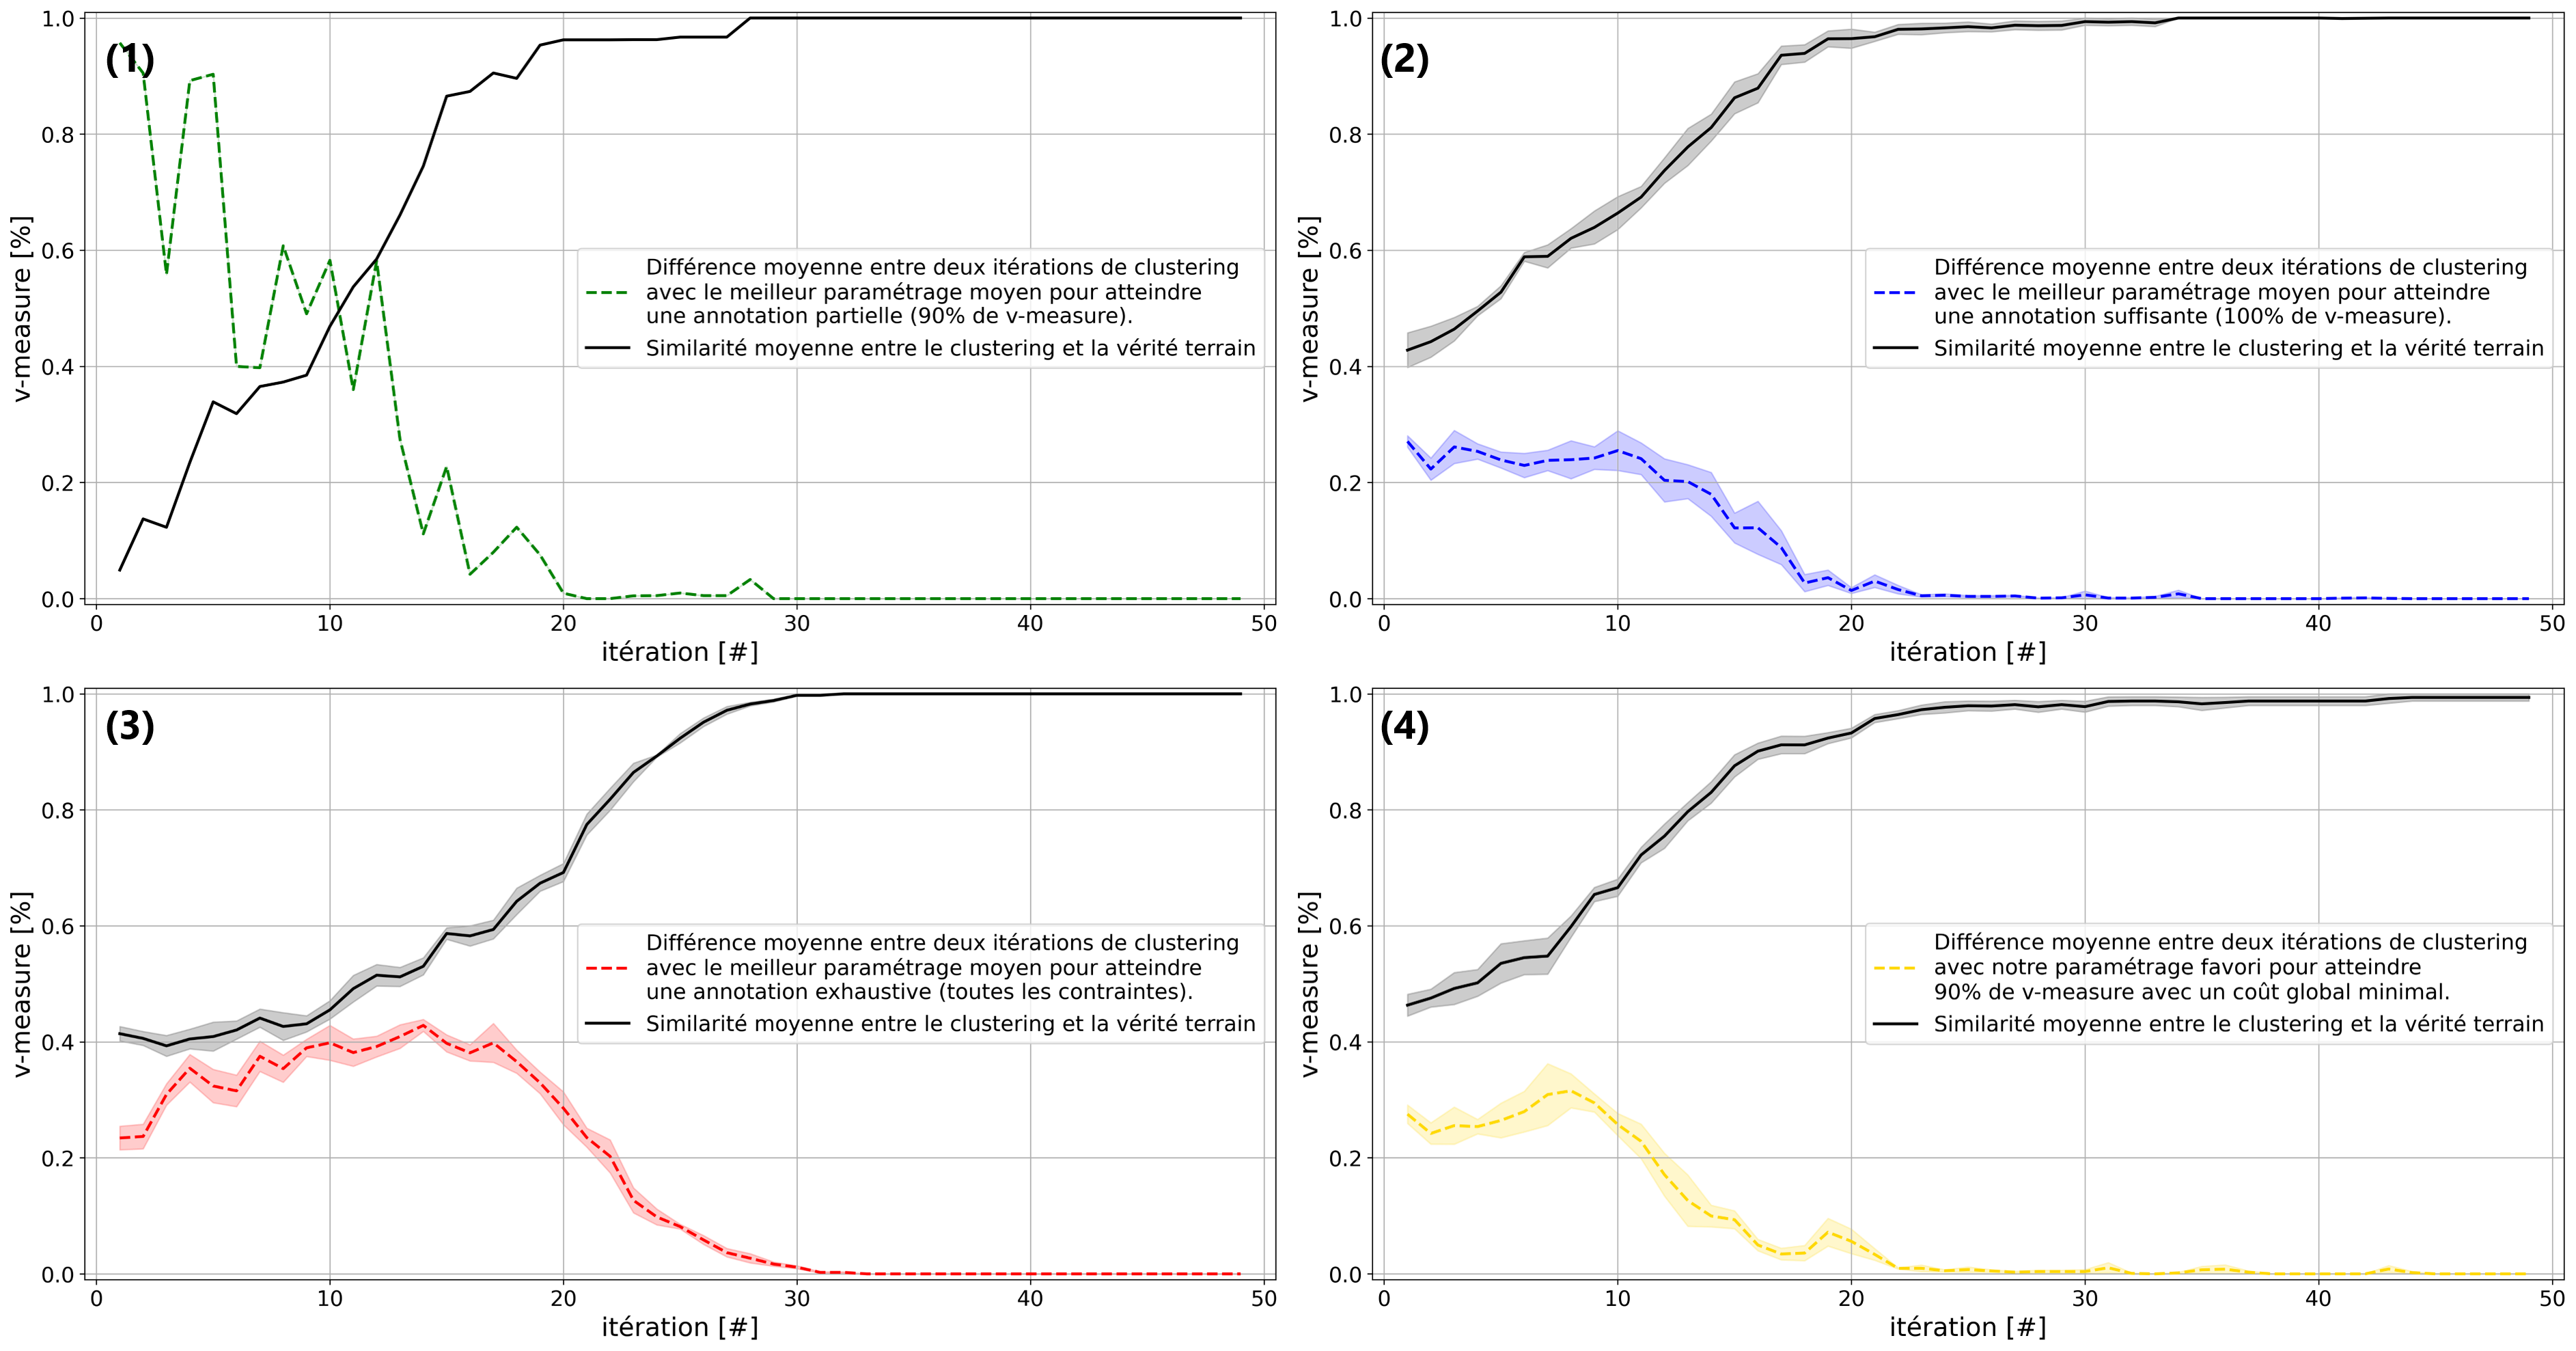
\includegraphics[width=0.95\textwidth]{figures/etude-rentabilite-similarite-clustering}
				\caption{
					Évolution de la différence de résultats entre deux itérations de \textit{clustering}.
					Les évolutions moyennes de différents paramétrages de la méthode sont exposées :
					\textbf{(1)} meilleur paramétrage moyen pour atteindre une annotation partielle ;
					\textbf{(2)} meilleur paramétrage moyen pour atteindre une annotation suffisante ;
					\textbf{(3)} meilleur paramétrage moyen pour atteindre une annotation exhaustive ;
					et \textbf{(4)} paramétrage favori.
					À titre d'information, les courbes en noir représentent l'évolution de la \texttt{v-measure} entre le \textit{clustering} et la vérité terrain.
				}
				\label{figure:4.5.2-ETUDE-RENTABILITE-SIMILARITE-CLUSTERING}
			\end{figure}
			
			% Tableau : corrélation forte.
			La \textsc{Table~\ref{table:4.5.2-ETUDE-RENTABILITE-CORRELATION-SIMILARITE-PERFORMANCE}} contient le score de corrélation entre cette différence et la performance théorique obtenue grâce à la vérité terrain.
			Cette corrélation est forte : $0.75$ sur l'ensemble des tentatives, $0.93$ sur les tentatives utilisant notre paramétrage favori.
			La \textsc{Figure~\ref{figure:4.5.2-ETUDE-RENTABILITE-SIMILARITE-CLUSTERING}} confirme cette corrélation :
			\begin{itemize}
				\item un score de \texttt{v-measure} avec la vérité terrain proche de $100$\% est accompagné d'un score de différence proche de $0$\% (après l'itération $20$ pour \textbf{(1)}, après l'itération $20$ pour \textbf{(2)}, après l'itération $30$ pour \textbf{(3)} et après l'itération $22$ pour \textbf{(4)}) ;
				\item une croissance de performance est généralement accompagnée d'un score non nul de différence (voir \textbf{(2)} et \textbf{(4)} entre les itérations $0$ et $20$), et plusieurs pics de performance sont accompagnés de scores forts de différence (particulièrement visible sur \textbf{(1)} vers l'itération $5$ et entre les itérations $10$ et $15$) ;
				\item il est toutefois à noter que l'inverse n'est pas vrai : un score non nul de différence n'accompagne pas forcément une croissance de performance, mais peut simplement caractériser un changement de partitionnement, comme c'est le cas dans \textbf{(3)} entre les itérations $0$ et $10$ où des modifications ont lieu (score de différence non nul) mais où la performance par rapport à la vérité terrain stagne.
			\end{itemize}
			%
			\begin{table}[!htb]
				\begin{center}
				\begin{tabular}{|c|r|}
				
					\hline
					% ENTETE DU TABLEAU
					\rowcolor{colorTableHeader!15}
					\multicolumn{1}{|c|}{\shortstack[c]{
						Paramétrage
					}}
						& \multicolumn{1}{c|}{\shortstack[c]{
							Corrélation
						}}
						\tabularnewline
						\hline \hline
					
					% Annotation partielle.
					Meilleur paramétrage moyen pour une annotation partielle \textbf{(1)}
						& $0.96$
						\tabularnewline
						\hline
					
					% Annotation suffisante.
					Meilleur paramétrage moyen pour une annotation suffisante \textbf{(2)}
						& $0.92$
						\tabularnewline
						\hline
					
					% Annotation exhaustive.
					Meilleur paramétrage moyen pour une annotation exhaustive \textbf{(3)}
						& $0.85$
						\tabularnewline
						\hline
					
					% Paramétrage favori
					Paramétrage favori \textbf{(4)}
						& $0.93$
						\tabularnewline
						\hline
					
					% Moyenne des $960$ tentatives.
					Moyenne des $960$ tentatives
						& $0.75$
						\tabularnewline
						\hline
					
				\end{tabular}
				\end{center}
				\caption{
					Score de corrélation \texttt{r} de \textit{Pearson} entre la performance du \textit{clustering} obtenu à l'aide d'une vérité terrain (\texttt{v-measure}) et le score de différence entre deux \textit{clustering} consécutifs.
				}
				\label{table:4.5.2-ETUDE-RENTABILITE-CORRELATION-SIMILARITE-PERFORMANCE}
			\end{table}
			
			% Description de la figure : autres paramétrages
			Les autres paramétrages représentés dans \textbf{(1)}, \textbf{(2)} et \textbf{(3)} comportent des tendances similaires (\textit{décroissance générale, forte corrélation avec la performance théorique}) à quelques détails près (\textit{\textbf{(1)} commence avec des scores de différence très forts avant de décroître avec de nombreux pics ; \textbf{(3)} croît légèrement avant d'entamer sa décroissance, ...}).
			
		%%% Discussion
		\subsubsection{Discussion}
		
			% Rappel de l'objectif : trouver un cas d'arrêt en regardant l'évolution de la différence entre deux \textit{clustering}.
			Dans cette étude, nous avons analysé l'évolution du score de différence entre deux itérations de \textit{clustering} dans l'espoir de définir un cas d'arrêt de notre méthodologie d'annotation qui soit indépendant d'une vérité terrain préétablie.
			
			% Avantage 1 : Caractérise la rentabilité.
			Tout d'abord, nous pouvons affirmer qu'il y a une forte corrélation entre l'évolution de ce score de différence et l'évolution du score de performance (voir \textsc{Table~\ref{table:4.5.2-ETUDE-RENTABILITE-CORRELATION-SIMILARITE-PERFORMANCE}} : \texttt{r} moyen de $0.75$ ; \texttt{r} supérieur à $0.85$ pour les paramétrages mis en avant).
			Cette corrélation est confirmée visuellement grâce à la \textsc{Figure~\ref{figure:4.5.2-ETUDE-RENTABILITE-SIMILARITE-CLUSTERING}} : plus les différences entre \textit{clustering} sont faibles, plus les performances des \textit{clustering} sont fortes.
			
			% Attention : Peut ne caractériser qu'un gros changement sans pour autant une amélioration.
			Un point d'attention est toutefois à retenir : une modification du partitionnement des données n'entraîne pas forcément un gain de performance (voir \textbf{(3)} entre les itérations $0$ et $10$ et \textbf{(4)} entre les itérations $0$ et $8$).
			Nous ne pouvons donc pas conclure que l'analyse de la différence entre deux itérations de \textit{clustering} permet de caractériser totalement la rentabilité d'une itération.
			
			% Avantage 2 : Permet de définir un cas d'arrêts.
			Cependant, nous pouvons tout de même nous servir de ce score pour définir un cas d'arrêt pour notre méthodologie d'annotation lorsque la différence entre deux \textit{clustering} est faible.
			Pour cela, il nous suffit de fixer un seuil bas du score de différence en dessous duquel il n'est plus rentable de faire de nouvelles itérations de la méthode car les performances ne s'améliorent plus significativement.
			Une analyse manuelle ou semi-manuelle (voir hypothèse de pertinence en \textsc{Section~\ref{section:4.4-HYPOTHESE-PERTINENCE}}) reste nécessaire pour confirmer la valeur métier du résultat obtenu.
			
			\begin{leftBarIdea}
				Si nous restons sur notre seuil théorique de $90$\% de \texttt{v-measure} (voir \textsc{Section~\ref{section:4.2-HYPOTHESE-EFFICIENCE}}) et que nous nous basons sur la \textsc{Figure~\ref{figure:4.5.2-ETUDE-RENTABILITE-SIMILARITE-CLUSTERING}} \textbf{(4)}, nous pouvons visuellement fixer ce seuil autour de $5$\% de différences.
				Le réglage fin de ce seuil pourra être le sujet de futures analyses complémentaires.
			\end{leftBarIdea}
			
			% Conclusions et suggestion.
			En conclusion, \textbf{le score de différences entre deux résultats de \textit{clustering} semble être un bon indicateur pour estimer un cas d'arrêt de notre méthodologie d'annotation}.
			Nous proposons d'utiliser un seuil par défaut de $5$\% pour implémenter ce cas d'arrêt.
			
	%%%
	%%% Subsection 4.5.3: Mise en commun des stratégies d'évaluation de la rentabilité d'une itération de la méthode et définition d'un cas d'arrêt indépendant d'une vérité terrain.
	%%%
	\subsection{Mise en commun des stratégies d'évaluation de la rentabilité d'une itération de la méthode et définition d'un cas d'arrêt indépendant d'une vérité terrain.}
	\label{section:4.5.3-ETUDE-RENTABILITE-MISE-EN-COMMUN}
			
		% Conclusion.
		\begin{leftBarSummary}
			Au cours de cette étude de rentabilité, nous avons pu voir que :
			\begin{itemize}
				\item[\itemko] l'analyse du score d'accord entre l'annotation courante et le \textit{clustering} précédent ne permet pas d'estimer la rentabilité d'une itération, ni de définir un cas d'arrêt de notre méthodologie d'annotation (cf. \textsc{Section~\ref{section:4.5.1-ETUDE-RENTABILITE-ACCORD-ANNOTATION-CLUSTERING}}) ;
				\item[\itemok] l'analyse des différences entre deux itérations de \textit{clustering} est une approche prometteuse pour estimer la rentabilité d'une itération (cf. \textsc{Section~\ref{section:4.5.2-ETUDE-RENTABILITE-SIMILARITE-CLUSTERING}}), bien qu'une modification significative entre deux résultats de \textit{clustering} n'implique pas forcément un gain de performance (\textit{les deux \textit{clustering} peuvent être différents mais avoir des \texttt{v-measure} avec la vérité terrain équivalentes}) ;
				\item[\itemok] l'usage de différences entre deux itérations de \textit{clustering} permet de définir un cas d'arrêt de notre méthodologie d'annotation : si les différences sont faibles (\textit{par exemple : inférieures à $5$\%}), alors les performances stagnent ou plafonnent ; il peut alors être intéressant d'interrompre le \texttt{Clustering Interactif} après avoir vérifié manuellement la pertinence des résultats obtenus (cf. \textsc{Section~\ref{section:4.4.4-ETUDE-PERTINENCE-MISE-EN-COMMUN}}).
			\end{itemize}
		\end{leftBarSummary}
		
		% Transition: Vers Simulation d'erreurs.
		Pour terminer nos différentes analyses, il convient maintenant d'anticiper la présence de différences d'annotation.
		En effet, nous avons fait jusqu'à présent l'hypothèse que l'annotateur ne se trompe jamais et que deux annotateurs n'ont jamais de désaccords, mais cette hypothèse forte n'est pas toujours vérifiée en pratique.
		Pour estimer l'impact de ces incohérences d'annotation, nous devons donc réaliser une analyse de robustesse de notre méthode d'annotation : celle-ci sera réalisée en \textsc{Section~\ref{section:4.6-HYPOTHESE-ROBUSTESSE}}.
	
	
	%%%%%--------------------------------------------------------------------
	%%%%% Section 4.6: Hypothèse de robustesse.
	%%%%%--------------------------------------------------------------------
	\newpage
	\section{Hypothèse de robustesse : « \textit{quelle influence d'une erreur ?} »}
\label{section:4.6-HYPOTHESE-ROBUSTESSE}

	%%% Formulation des hypothèses:
	Nous aimerions vérifier l'hypothèse suivante :
	\todo{à reformuler}

	\begin{tcolorbox}[
		title=\faVial~\textbf{Hypothèse de robustesse}~\faVial,
		colback=colorTcolorboxHypothesis!15,  % gray!20
		colframe=colorTcolorboxHypothesis!75,  % gray!50!black!75,
		width=\linewidth
	]
		« Il est possible d'\textbf{estimer l'influence d'une différence d'annotation} lors d'une méthodologie d'annotation basée sur le \textit{clustering} interactif (cf. figure~\ref{figure:4.6-HYPOTHESE-ROBUSTESSE}. »
		
		
		\begin{figure}[H]  % keep [H] to be in the tcolorbox.
			\centering
			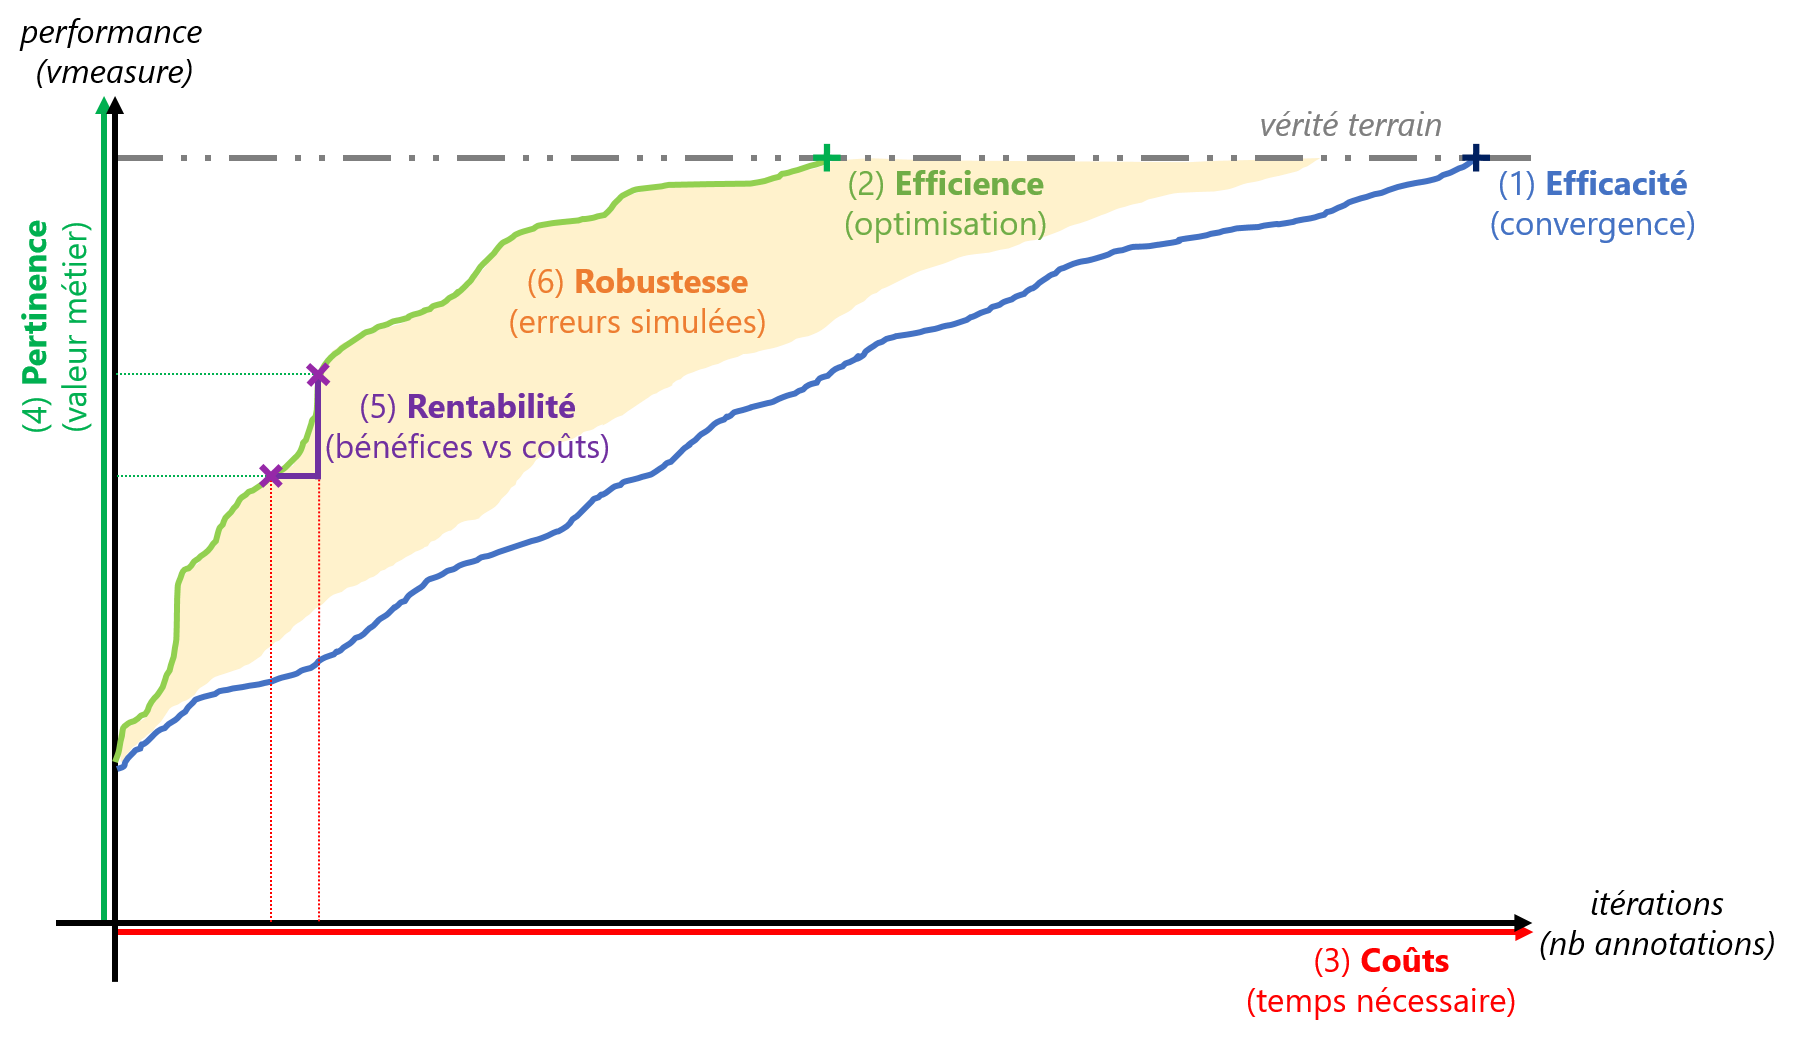
\includegraphics[width=0.95\textwidth]{figures/hypotheses-06-robustesse}
			\caption{Illustration des études réalisées sur le \textit{clustering} interactif (\textit{étape 6/6}) en schématisant l'évolution de la performance (\textit{accord avec la vérité terrain calculé en v-measure}) d'une base d'apprentissage en cours de construction en fonction du nombre d'itérations de la méthode (\textit{nombre d'annotations par un expert métier}).}
			\label{figure:4.6-HYPOTHESE-ROBUSTESSE}
		\end{figure}

	\end{tcolorbox}
	
	%%%
	%%% Subsection 4.6.1: Étude de simulation d'erreurs d'annotations
	%%%
	\subsection{Étude de simulation d'erreurs d'annotations}
	
		%%% Protocole expérimental.
		\subsubsection{Protocole expérimental}
			\todo[inline]{Description succincte du protocole expérimental dans l'encadré d'hypothèse ?}

		%%% Résultats
		\subsubsection{Résultats obtenus}

		%%% Discussion
		\subsubsection{Discussion}
	
	%%%
	%%% Subsection 4.6.2: Étude d'annotation avec des paradigmes différents
	%%%
	\subsection{Étude d'annotation avec des paradigmes différents}
	
		%%% Protocole expérimental.
		\subsubsection{Protocole expérimental}
			\todo[inline]{Description succincte du protocole expérimental dans l'encadré d'hypothèse ?}

		%%% Résultats
		\subsubsection{Résultats obtenus}

		%%% Discussion
		\subsubsection{Discussion}
	
	
	%%%%%--------------------------------------------------------------------
	%%%%% Section 4.7: Hypothèses non vérifiées.
	%%%%%--------------------------------------------------------------------
	\newpage
	\section{Autres hypothèses non vérifiées}
\label{section:4.7-HYPOTHESES-NON-VERIFIEES}

	%%%
	%%% Introduction / Transition.
	%%%
	Lors des études précédentes, nous avons vérifié un certain nombre d'hypothèses et avons exploré plusieurs détails pratiques pour mettre en oeuvre une méthodologie d'annotation basée sur le \textit{clustering} interactif.
	Toutefois, certains points n'ont pas pu être étudiés en profondeurs lors de ce doctorat, par manque de temps ou de moyens.
	Nous exposons ici un ensemble de pistes intéressantes pouvant nourrir de futurs travaux afin d'améliorer la notre méthode.
	
	
	%%%
	%%% Subsection 4.7.1: Étude du nombre de clusters optimal.
	%%%
	\subsection{Étude du nombre de clusters optimal}
	\label{section:4.7.1-HYPOTHESES-NON-VERIFIEES-NOMBRE-CLUSTERS}
	
		% Problème ouvert de la recherche: Estimer le nombre optimal de clusters.
		Un problème ouvert de la recherche lors de l'utilisation d'algorithmes de \textit{clustering} concerne le choix du nombre de \textit{clusters} à trouver.
		En effet, à part une connaissance à priori du nombre de thématiques présentes dans le jeu de données, il est difficile d'estimer le nombre optimal de \textit{clusters}, d'autant plus que celui-ci peut changer en fonction de la granularité de modélisation requise pour répondre au cas d'usage.
		
		% Pistes déjà explorées.
		Nous avons déjà exploré partiellement deux pistes :
		\begin{itemize}
			\item l'\textbf{exploration du graphe de contraintes} : en effet, il est possible d'estimer le nombre maximal de \textit{clusters} grâce aux composants connexes de contraintes \texttt{MUST-LINK}, et d'estimer le nombre minimal de \textit{clusters} grâce à la coloration du graphe de contraintes \texttt{CANNOT-LINK} ;
			\item les \textbf{études de pertinence} avec l'analyse des patterns linguistiques et le résumé thématique des \textit{clusters} (cf. \textsc{Section~\ref{section:4.4-HYPOTHESE-PERTINENCE}}) : ces deux approches permettent de rapidement constater si les thématiques obtenues sont trop générales (\textit{i.e. s'il n'y a pas assez de clusters}) ou si elles semblent trop spécifiques (\textit{i.e. s'il y en a trop}).
		\end{itemize}
		
		% Piste potentielles à explorer.
		Toutefois, pour aller plus loin, deux pistes potentielles pourraient être explorées :
		\begin{itemize}
			\item l'exploration brute du nombre de \textit{clusters} par la \textbf{méthode du coude} : bien que ces approches sont plus coûteuses en temps de calcul, elles permettent d'estimer le nombre de \textit{clusters} pour lequel la stabilité du \textit{clustering} est la plus élevée ;
			\item l'utilisation d'algorithme n'ayant pas de nombre de clusters en paramètres comme des versions contraintes de \texttt{DBScan} (par exemple dans sa version \texttt{C-DBScan}, \cite{ruiz-etal:2010:densitybased-semisupervised-clustering}) ou de la \textbf{propagation par affinité} (\cite{givoni-frey:2009:semisupervised-affinity-propagation}) : ces alternatives semblent prometteuses car elles retirent la complexité due à ce paramétrage abstrait.
		\end{itemize}
		
		\setcounter{localCounterOfFootnoteValue}{\value{footnote}}
		\begin{leftBarInformation}
			L'étude de \texttt{C-DBScan} a été en partie réalisée dans le cadre d'un projet étudiant avec l'école d'ingénieur Télécom Physique Strasbourg.
			Les résultats montraient que le temps de calcul était similaire à celui du \texttt{KMeans} (dans sa version \texttt{COP}).
			La difficulté d'utilisation résidait plutôt sur la définition du rayon de voisinage \texttt{eps} à parcourir pour établir des liens entre données.
			Celui-ci peut être estimé en analysant la densité vectorielle du jeu de données.
			Le code informatique est disponible dans \cite{schild:2022:cognitivefactory-interactiveclustering} \footnotemark.
		\end{leftBarInformation}
		% Rattraper les footnote.
			\stepcounter{localCounterOfFootnoteValue}
			\footnotetext[\value{localCounterOfFootnoteValue}]{
				Implémentation de \texttt{C-DBScan} : \textit{Pull Request} en attente pour une version \texttt{0.6.0} après ajout de documentation et de tests unitaires.
			}
	
	
	%%%
	%%% Subsection 4.7.2: Étude d'autres méthodes de vectorisation.
	%%%
	\subsection{Étude d'autres méthodes de vectorisation}
	\label{section:4.7.2-HYPOTHESES-NON-VERIFIEES-VECTORISATION}
	
		% Introduction.
		Au début de ce doctorat, nous avons conclu que les algorithmes de vectorisation n'avaient pas d'impact réel sur l'efficience de notre méthodologie d'annotation.
		Toutefois, les modèles de langues se sont largement développés, et il est fort probable que l'utilisation d'un \textbf{modèle pré-entraîné} permettent désormais d'avoir un gain de performance.
		
		% Piste potentielles à explorer.
		Nous pourrions par exemple tester les \textbf{architectures à base de \textit{Transformers}} (\cite{uszkoreit:2017:transformer-novel-neural}) comme \texttt{BERT} (\cite{devlin-etal:2019:bert-pretraining-deep}) et essayer différents modèles pré-entraînés sur des données françaises pour compléter nos études réalisées dans \cite{schild:2021:cognitivefactory-interactiveclusteringcomparativestudy}
	
	
	%%%
	%%% Subsection 4.7.3: Étude d'autres méthodes d'échantillonnage.
	%%%
	\subsection{Étude d'autres méthodes d'échantillonnage}
	\label{section:4.7.3-HYPOTHESES-NON-VERIFIEES-ECHANTILLONNAGE}
	
		% Introduction.
		Comme nous avons pu le voir dans \textsc{Section~\ref{section:4.6-HYPOTHESE-ROBUSTESSE}}, il peut-être intéressant d'introduire un mécanisme de création de redondance dans le graphe de contraintes annotées pour identifier les erreurs d'annotation.
		Un tel mécanisme n'a pas encore été implémenté mais pourrait facilement être intégré aux implémentations \texttt{Python} déjà existantes (\cite{schild:2022:cognitivefactory-interactiveclustering}).
		
		% Piste potentielles à explorer.
		Pour ce faire, le parcours de graphe et la création de cycle permettraient de vérifier la présence de conflits et ainsi de \textbf{provoquer des phases de revues de contraintes} si cela est nécessaire.
		Une telle page de revue pourrait aussi être complétée par des analyses complémentaires, comme l'estimation du taux de contraintes n'ayant pas de redondance et représentant ainsi des erreurs cachées potentielles.
	
	
	%%%
	%%% Subsection 4.7.4: Étude de techniques de transfert d'apprentissage.
	%%%
	\subsection{Étude de techniques de transfert d'apprentissage}
	\label{section:4.7.4-HYPOTHESES-NON-VERIFIEES-TRANSFERT-APPRENTISSAGE}
	
		% Introduction.
		Dans la \textsc{Section~\ref{section:2.3-DEFIS-ANNOTATION}}, nous avions déjà évoqué le fait que la modélisation d'un phénomène peut être assister par des techniques telles que la pré-annotation (\cite{dandapat-etal:2009:complex-linguistic-annotation}) ou le transfert d'apprentissage (\cite{zhuang-etal:2021:comprehensive-survey-transfer}).
		Nous pourrions nous inspirer davantage de ces approches pour démarrer plus efficacement les premières itérations d'un \textit{clustering} interactif.
	
		% Piste potentielles à explorer.
		Voici quelques idées inspirées de ces méthodes :
		\begin{itemize}
			\item \textbf{pré-annoter} certaines contraintes simples à l'aide de règles (\textit{basées par exemple sur la présence de mots de vocabulaire en commun}) ou grâce à l'utilisation d'un modèle déjà disponible ; 
			\item \textbf{introduire des données synthétiques ou empruntées} à d'autres bases d'apprentissage pour initialiser le \textit{clustering}, et permettre ainsi ajouter d'emblée des connaissances générales dans la modélisation.
		\end{itemize}
	
	
	%%%
	%%% Subsection 4.7.5: Étude ergonomique de l'interface d'annotation.
	%%%
	\subsection{Étude ergonomique de l'interface d'annotation}
	\label{section:4.7.5-HYPOTHESES-NON-VERIFIEES-ERGONOMIQUE}
	
		% Introduction.
		L'application web développée au cours de ce doctorat (\cite{schild-etal:2022:cognitivefactory-interactiveclusteringgui}) permet d'essayer rapidement notre méthodologie d'annotation.
		Cependant, cette dernière n'a pu faire l'objet d'études poussées pour estimer la meilleure disposition des composants ou l'intérêt de certaines fonctionnalités d'annotation.
		
		% Piste potentielles à explorer.
		Parmi les pistes potentielles à explorer, nous avons évoqué la possibilité d'\textbf{annoter plusieurs contraintes} dans une même interface (\textit{par exemple : annoter visuellement un mini-graphes de $4$ données plutôt que d'annoter simplement un couple de données}) et le besoin de \textbf{réaliser des analyses rapides} sur les \textit{clusters} ou sur le graphe de contraintes (voir \textsc{Section~\ref{section:4.4-HYPOTHESE-PERTINENCE}} et \textsc{Section~\ref{section:4.5-HYPOTHESE-RENTABILITE}}).
		Pour aller plus loin, \cite{bae-etal:2021:interactive-clustering-comprehensive} propose d'autres listes d'interactions qui sont possibles d'avoir avec un algorithmes de \textit{clustering}, notamment sur la manipulation de son résultats (\textit{fusion, suppression, verrouillage, ...}) et de ses hyperparamètres (\textit{nombre de \textit{clusters}, adaptation du vocabulaire autorisé, ...})
		
		% A essayer !
		Toutes ces idées pourraient être l'objet de développements et d'études dédiées avec des groupes d'annotateurs différentes pour voir l'impact sur les performances et les biais de conception de modèles.
	
	
	%%%%%--------------------------------------------------------------------
	%%%%% Section 4.8: Bilan des études réalisées
	%%%%%--------------------------------------------------------------------
	\newpage
	\section{Bilan des études réalisées}
\label{section:4.8-BILAN-HYPOTHESES}
	\todo[inline]{SECTION À RÉDIGER}
	
	% FONCTIONNALITES
		% trouver une base d'apprentissage acceptable, puis corriger manuellement
		% intervention d'experts métiers sur la base de leur connaissance métiers
		% revues d'annotations basée sur leur connaissance métiers
		% adaptation de la modélisation faite par le clustering
	
	% PARAMETRAGES
		% Architecture parallele :
		% paramétrage :
		% batch_size :
	
	% ANALYSE
		% Cas d'arrêt quand le clustering stage à +/- 5%
		% Analyse avec FMC + résumé LLM
	
	% COUTS
		% equations de temps
		% besoin de 3 annotateurs
		% ajouter de la redondance si le cas d'usage est complexe